%%%%%%%%%%%%%%%%%%%%%%%%%%%%%%%%%%%%%%%%%
% Classicthesis Typographic Thesis
% LaTeX Template
% Version 1.4 (1/1/16)
%
% This template has been downloaded from:
% http://www.LaTeXTemplates.com
%
% Original author:
% André Miede (http://www.miede.de) with commenting modifications by:
% Vel (vel@LaTeXTemplates.com)
%
% License:
% GNU General Public License (v2)
%
% General Tips:
% 1) Make sure to edit the classicthesis-config.file
% 2) New enumeration (A., B., C., etc in small caps): \begin{aenumerate} \end{aenumerate}
% 3) For margin notes: \marginpar or \graffito{}
% 4) Do not use bold fonts in this style, it is designed around them
% 5) Use tables as in the examples
% 6) See classicthesis-preamble.sty for useful commands
%
%%%%%%%%%%%%%%%%%%%%%%%%%%%%%%%%%%%%%%%%%

%----------------------------------------------------------------------------------------
%	PACKAGES AND OTHER DOCUMENT CONFIGURATIONS
%----------------------------------------------------------------------------------------

\documentclass[
		twoside,openright,titlepage,numbers=noenddot,headinclude,%1headlines,
	 	footinclude=false,cleardoublepage=empty,
		dottedtoc, % Make page numbers in the table of contents flushed right with dots leading to them
		BCOR=5mm,paper=a4,fontsize=11pt, % Binding correction, paper type and font size
		ngerman,american, % Languages, change this to your language(s)
		]{scrreprt}

% Includes the file which contains all the document configurations and packages - make sure to edit this file
%%%%%%%%%%%%%%%%%%%%%%%%%%%%%%%%%%%%%%%%%
% Classicthesis Typographic Thesis
% Configuration File
%
% This file has been downloaded from:
% http://www.LaTeXTemplates.com
%
% Original author:
% André Miede (http://www.miede.de) with extensive commenting changes by:
% Vel (vel@LaTeXTemplates.com)
%
% License:
% GNU General Public License (v2)
%
% Important note:
% The main lines to change in this file are in the DOCUMENT VARIABLES
% section, the rest of the file is for advanced configuration.
%
%%%%%%%%%%%%%%%%%%%%%%%%%%%%%%%%%%%%%%%%%

%----------------------------------------------------------------------------------------
%	CHARACTER ENCODING
%----------------------------------------------------------------------------------------

\PassOptionsToPackage{utf8}{inputenc} % Set the encoding of your files. UTF-8 is the only sensible encoding nowadays. If you can't read äöüßáéçèê∂åëæƒÏ€ then change the encoding setting in your editor, not the line below. If your editor does not support utf8 use another editor!
\usepackage{inputenc}

%----------------------------------------------------------------------------------------
%	DOCUMENT VARIABLES
%	Fill in the lines below to enter your information into the thesis template
%	Each of the commands can be cited anywhere in the thesis
%----------------------------------------------------------------------------------------

% Remove drafting to get rid of the '[ Date - classicthesis version 4.0 ]' text at the bottom of every page
\PassOptionsToPackage{eulerchapternumbers,listings,drafting, pdfspacing, subfig,beramono,eulermath,parts}{classicthesis}
% Available options: drafting parts nochapters linedheaders eulerchapternumbers beramono eulermath pdfspacing minionprospacing tocaligned dottedtoc manychapters listings floatperchapter subfig

\newcommand{\myTitle}{Multiplicities of hadrons in Deep-Inelastic Scattering of muons on nucleons at COMPASS\xspace}
\newcommand{\mySubtitle}{\xspace}
\newcommand{\myDegree}{Doctor\xspace}
\newcommand{\myName}{Nicolas Pierre\xspace}
\newcommand{\myProf}{Put name here\xspace}
\newcommand{\myOtherProf}{Put name here\xspace}
\newcommand{\mySupervisor}{Dr. Fabienne Kunne\xspace}
\newcommand{\myFaculty}{Université Paris-Saclay\xspace}
\newcommand{\myDepartment}{CEA-Irfu/DPhN\xspace}
\newcommand{\myUni}{Johannes-Gutenberg Universitaet Mainz\xspace}
\newcommand{\myLocation}{Saclay\xspace}
\newcommand{\myTime}{March 2019\xspace}
\newcommand{\myVersion}{}

%----------------------------------------------------------------------------------------
%	USEFUL COMMANDS
%----------------------------------------------------------------------------------------

\newcommand{\ie}{i.\,e.}
\newcommand{\Ie}{I.\,e.}
\newcommand{\eg}{e.\,g.}
\newcommand{\Eg}{E.\,g.}

\newcounter{dummy} % Necessary for correct hyperlinks (to index, bib, etc.)
\providecommand{\mLyX}{L\kern-.1667em\lower.25em\hbox{Y}\kern-.125emX\@}
\newlength{\abcd} % for ab..z string length calculation

%----------------------------------------------------------------------------------------
%	PACKAGES
%----------------------------------------------------------------------------------------

\usepackage{lipsum} % Used for inserting dummy 'Lorem ipsum' text into the template

%------------------------------------------------

%\PassOptionsToPackage{ngerman,american}{babel}  % Change this to your language(s)
% Spanish languages need extra options in order to work with this template
%\PassOptionsToPackage{spanish,es-lcroman}{babel}
\usepackage{babel}

%------------------------------------------------

\usepackage{csquotes}
\PassOptionsToPackage{%
%backend=biber, % Instead of bibtex
backend=bibtex8,bibencoding=ascii,%
language=auto,%
style=numeric-comp,%
%style=authoryear-comp, % Author 1999, 2010
%bibstyle=authoryear,dashed=false, % dashed: substitute rep. author with ---
sorting=nyt, % name, year, title
maxbibnames=10, % default: 3, et al.
%backref=true,%
natbib=true % natbib compatibility mode (\citep and \citet still work)
}{biblatex}
\usepackage{biblatex}

 %------------------------------------------------

\PassOptionsToPackage{fleqn}{amsmath} % Math environments and more by the AMS
 \usepackage{amsmath}

 %------------------------------------------------

\PassOptionsToPackage{T1}{fontenc} % T2A for cyrillics
\usepackage{fontenc}

%------------------------------------------------

\usepackage{textcomp} % Fix warning with missing font shapes

%------------------------------------------------

\usepackage{scrhack} % Fix warnings when using KOMA with listings package

%------------------------------------------------

\usepackage{xspace} % To get the spacing after macros right

%------------------------------------------------

\usepackage{mparhack} % To get marginpar right

%------------------------------------------------

\usepackage{fixltx2e} % Fixes some LaTeX stuff

%------------------------------------------------

\PassOptionsToPackage{smaller}{acronym} % Include printonlyused in the first bracket to only show acronyms used in the text
\usepackage{acronym} % Nice macros for handling all acronyms in the thesis

%\renewcommand*{\acsfont}[1]{\textssc{#1}} % For MinionPro
\renewcommand*{\aclabelfont}[1]{\acsfont{#1}}

%------------------------------------------------

\PassOptionsToPackage{pdftex}{graphicx}
\usepackage{graphicx}

%----------------------------------------------------------------------------------------
%	FLOATS: TABLES, FIGURES AND CAPTIONS SETUP
%----------------------------------------------------------------------------------------

\usepackage{tabularx} % Better tables
\setlength{\extrarowheight}{3pt} % Increase table row height
\newcommand{\tableheadline}[1]{\multicolumn{1}{c}{\spacedlowsmallcaps{#1}}}
\newcommand{\myfloatalign}{\centering} % To be used with each float for alignment
\usepackage{caption}
\captionsetup{font=small}
\usepackage{subfig}

%----------------------------------------------------------------------------------------
%	CODE LISTINGS SETUP
%----------------------------------------------------------------------------------------

\usepackage{listings}
%\lstset{emph={trueIndex,root},emphstyle=\color{BlueViolet}}%\underbar} % For special keywords
\lstset{language=[LaTeX]Tex,%C++ % Specify the language(s) for listings here
morekeywords={PassOptionsToPackage,selectlanguage},
keywordstyle=\color{RoyalBlue}, % Add \bfseries for bold
basicstyle=\small\ttfamily, % Makes listings a smaller font size and a different font
%identifierstyle=\color{NavyBlue}, % Color of text inside brackets
commentstyle=\color{Green}\ttfamily, % Color of comments
stringstyle=\rmfamily, % Font type to use for strings
numbers=left, % Change left to none to remove line numbers
numberstyle=\scriptsize, % Font size of the line numbers
stepnumber=5, % Increment of line numbers
numbersep=8pt, % Distance of line numbers from code listing
showstringspaces=false, % Sets whether spaces in strings should appear underlined
breaklines=true, % Force the code to stay in the confines of the listing box
%frameround=ftff, % Uncomment for rounded frame
%frame=single, % Frame border - none/leftline/topline/bottomline/lines/single/shadowbox/L
belowcaptionskip=.75\baselineskip % Space after the "Listing #: Desciption" text and the listing box
}

%----------------------------------------------------------------------------------------
%	HYPERREFERENCES
%----------------------------------------------------------------------------------------

\PassOptionsToPackage{pdftex,hyperfootnotes=false,pdfpagelabels}{hyperref}
\usepackage{hyperref}  % backref linktocpage pagebackref
\pdfcompresslevel=9
\pdfadjustspacing=1

\hypersetup{
% Uncomment the line below to remove all links (to references, figures, tables, etc), useful for b/w printouts
%draft,
colorlinks=true, linktocpage=true, pdfstartpage=3, pdfstartview=FitV,
% Uncomment the line below if you want to have black links (e.g. for printing black and white)
%colorlinks=false, linktocpage=false, pdfborder={0 0 0}, pdfstartpage=3, pdfstartview=FitV,
breaklinks=true, pdfpagemode=UseNone, pageanchor=true, pdfpagemode=UseOutlines,%
plainpages=false, bookmarksnumbered, bookmarksopen=true, bookmarksopenlevel=1,%
hypertexnames=true, pdfhighlight=/O,%nesting=true,%frenchlinks,%
urlcolor=webbrown, linkcolor=RoyalBlue, citecolor=webgreen, %pagecolor=RoyalBlue,%
    %urlcolor=Black, linkcolor=Black, citecolor=Black, %pagecolor=Black,%
%------------------------------------------------
% PDF file meta-information
pdftitle={\myTitle},
pdfauthor={\textcopyright\ \myName, \myUni, \myFaculty},
pdfsubject={},
pdfkeywords={},
pdfcreator={pdfLaTeX},
pdfproducer={LaTeX with hyperref and classicthesis}
%------------------------------------------------
}

%----------------------------------------------------------------------------------------
%	AUTOREFERENCES SETUP
%	Redefines how references in text are prefaced for different
%	languages (e.g. "Section 1.2" or "section 1.2")
%----------------------------------------------------------------------------------------

\makeatletter
\@ifpackageloaded{babel}
{
\addto\extrasamerican{
\renewcommand*{\figureautorefname}{Figure}
\renewcommand*{\tableautorefname}{Table}
\renewcommand*{\partautorefname}{Part}
\renewcommand*{\chapterautorefname}{Chapter}
\renewcommand*{\sectionautorefname}{Section}
\renewcommand*{\subsectionautorefname}{Section}
\renewcommand*{\subsubsectionautorefname}{Section}
}
\addto\extrasngerman{
\renewcommand*{\paragraphautorefname}{Absatz}
\renewcommand*{\subparagraphautorefname}{Unterabsatz}
\renewcommand*{\footnoteautorefname}{Fu\"snote}
\renewcommand*{\FancyVerbLineautorefname}{Zeile}
\renewcommand*{\theoremautorefname}{Theorem}
\renewcommand*{\appendixautorefname}{Anhang}
\renewcommand*{\equationautorefname}{Gleichung}
\renewcommand*{\itemautorefname}{Punkt}
}
\providecommand{\subfigureautorefname}{\figureautorefname} % Fix to getting autorefs for subfigures right
}{\relax}
\makeatother

%----------------------------------------------------------------------------------------

\usepackage{classicthesis}
\usepackage{tikz}
\usepackage[absolute]{textpos}
\usepackage{epsfig}
\usepackage{color}
\usepackage{varwidth}
\usepackage{verbatim}
\usepackage{hyperref}

%----------------------------------------------------------------------------------------
%	CHANGING TEXT AREA
%----------------------------------------------------------------------------------------

\linespread{1.05} % a bit more for Palatino
\areaset[current]{450pt}{761pt} % 686 (factor 2.2) + 33 head + 42 head \the\footskip
\setlength{\marginparwidth}{2em}%
\setlength{\marginparsep}{1em}%

%----------------------------------------------------------------------------------------
%	USING DIFFERENT FONTS
%----------------------------------------------------------------------------------------

%\usepackage[oldstylenums]{kpfonts} % oldstyle notextcomp
%\usepackage[osf]{libertine}
%\usepackage[light,condensed,math]{iwona}
%\renewcommand{\sfdefault}{iwona}
%\usepackage{lmodern} % <-- no osf support :-(
%\usepackage{cfr-lm} %
%\usepackage[urw-garamond]{mathdesign} <-- no osf support :-(
%\usepackage[default,osfigures]{opensans} % scale=0.95
%\usepackage[sfdefault]{FiraSans}


\addbibresource{Bibliography.bib} % The file housing your bibliography
%\addbibresource[label=ownpubs]{Self_Publications.bib} % Uncomment for optional self-publications

%\hyphenation{Put special hyphenation here}

\begin{document}

\frenchspacing % Reduces space after periods to make text more compact

\raggedbottom % Makes all pages the height of the text on that page

\selectlanguage{american} % Select your default language - e.g. american or ngerman

%\renewcommand*{\bibname}{new name} % Uncomment to change the name of the bibliography
%\setbibpreamble{} % Uncomment to include a preamble to the bibliography - some text before the reference list starts

\pagenumbering{roman} % Roman page numbering prior to the start of the thesis content (i, ii, iii, etc)

\pagestyle{plain} % Suppress headers for the pre-content pages

%----------------------------------------------------------------------------------------
%	PRE-CONTENT THESIS PAGES
%----------------------------------------------------------------------------------------

% Title Page

\begin{titlepage}

\begin{addmargin}[-1cm]{-3cm}
\begin{center}
\large

\hfill
\vfill

\begingroup
\color{Maroon}\spacedallcaps{\myTitle} \\ \bigskip % Thesis title
\endgroup

\spacedlowsmallcaps{\myName} % Your name

\vfill

% 
\includegraphics[width=6cm]{gfx/TFZsuperellipse_bw} \\ \medskip % Picture

\medskip % Thesis subtitle
\myDegree \\
\myDepartment \\
\myFaculty \\
\myUni \\ \bigskip

% \myTime\ -- \myVersion % Time and version

\vfill

\end{center}
\end{addmargin}

\end{titlepage}
 % Main title page

% Back of the title page

\thispagestyle{empty}

\hfill

\vfill

\noindent\myName: \textit{\myTitle,} %\myDegree, 
\textcopyright\ \myTime

% You may wish to do something with the back of the title page, such as including your supervisors, location or time frame of the work. Below is an example of doing so although you may want to tweak it to your liking.

%\bigskip

%\noindent\spacedlowsmallcaps{Supervisors}: \\
%\myProf \\
%\myOtherProf \\
%\mySupervisor

%\medskip \\

%\noindent\spacedlowsmallcaps{Location}: \\
%\myLocation

%\medskip \\

%\noindent\spacedlowsmallcaps{Time Frame}: \\
%\myTime
 % Back of the title page

\cleardoublepage% Abstract

%\renewcommand{\abstractname}{Abstract} % Uncomment to change the name of the abstract

\pdfbookmark[1]{Abstract}{Abstract} % Bookmark name visible in a PDF viewer

\begingroup
\let\clearpage\relax
\let\cleardoublepage\relax
\let\cleardoublepage\relax

\chapter*{Abstract}
Short summary of the contents\dots a great guide by 
Kent Beck how to write good abstracts can be found here:  
\begin{center}
\url{https://plg.uwaterloo.ca/~migod/research/beckOOPSLA.html}
\end{center}

\endgroup			

\vfill % Abstract page

%\cleardoublepage\include{FrontBackMatter/Foreword} % Uncomment and create a Foreword.tex to include a foreword

% \cleardoublepage% Publications - a page listing research articles written using content in the thesis

\pdfbookmark[1]{Publications}{Publications} % Bookmark name visible in a PDF viewer

\chapter*{Publications} % Publications page text

Some ideas and figures have appeared previously in the following publications:\\

\noindent Put your publications from the thesis here. The packages \texttt{multibib} or \texttt{bibtopic} etc. can be used to handle multiple different bibliographies in your document.

%\begin{refsection}[ownpubs]
%    \small
%    \nocite{*} % is local to to the enclosing refsection
%    \printbibliography[heading=none]
%\end{refsection}

%\emph{Attention}: This requires a separate run of \texttt{bibtex} for your \texttt{refsection}, \eg, \texttt{ClassicThesis1-blx} for this file. You might also use \texttt{biber} as the backend for \texttt{biblatex}. See also \url{http://tex.stackexchange.com/questions/128196/problem-with-refsection}. % Publications from the thesis page

\cleardoublepage% Dedication

\thispagestyle{empty}
\refstepcounter{dummy}

\pdfbookmark[1]{Dedication}{Dedication} % Bookmark name visible in a PDF viewer

\vspace*{3cm}

\begin{center}
\emph{Ohana} means family. \\
Family means nobody gets left behind, or forgotten. \\ \medskip
--- Lilo \& Stitch    
\end{center}

\medskip

\begin{center}
Dedicated to the loving memory of Rudolf Miede. \\ \smallskip
1939\,--\,2005
\end{center} % Dedication page

\cleardoublepage% Acknowledgements

\pdfbookmark[1]{Acknowledgements}{Acknowledgements} % Bookmark name visible in a PDF viewer


\bigskip

%----------------------------------------------------------------------------------------

\begingroup

\let\clearpage\relax
\let\cleardoublepage\relax
\let\cleardoublepage\relax

\chapter*{Acknowledgements}

First and foremost, I would like to thank CEA/IRFU and particularly the DPhN, the University of Mainz and particularly the KPH, and the COMPASS collaboration. That is with them that this whole story started.

I would like to then thank my two thesis directors, Fabienne Kunne and Eva-Maria Kabuß, for giving me the opportunity to become a PhD student, for always being present to guide me and always conforting me in my choices.

I would like to express my gratitude to the members of my jury. I would like to thank Franck Sabatié for agreeing to head the jury and also for the great support he has been during my year-ish in Saclay. The discussion with Andrea Bressan were always interesting and elevating. The moments with Fritz Klein at the Bonn meeting every Christmas were always a pleasure. I would eventually express my deepest appreciation to Hubert Spiesberger that helped me so much with the theory behind all the radiative corrections and was so nice and pedagogical in any circumstance.

Ich danke meinen COMPASS-Mainz Kollegen Johannes, Moritz, Malte und Nick. Es war wirklich eine Freude, mit Ihnen in Mainz und anderswo zusammen zu sein. Ich war der 'Petit Français' des Teams mit allen Klischees, aber Sie haben mich trotzdem als Teil des Teams begrüßt.

Je voudrais aussi remercier mes collègue de COMPASS à Saclay, que ce soit Damien, Stéphane ou Yann. Les discussions que nous avons eu sur la physique ou même des thèmes plus variés ont toujours été un plaisir. Merci à toi Nicole d'avoir été comme ma troisième directrice de thèse dans les derniers mois, j'aurais été dans la panade sans ton aide !

Special thanks for all the COMPASS collaboration members. Thanks to Riccardo, Jan, Misha, Andrea, Bakur, it was always great to discuss with you in and outside work. Thanks to Marcin for the always high-spirited and brilliant discussions we had, live of by email. You are never short of ideas and that is pretty impressive.

Ich möchte mich bei Manfred und Margrit bedanken, die mich für 2 Jahre in ihrem Haus in Mainz begrüßen durften. Sie haben meinen Aufenthalt in Deutschland deutlich verbessert!

J'aimerais remercier l'ensemble des précaires du DPhN. On était tous dans la même galère, on en est tous sorti en se serrant les coudes dans la bonne humeur. Toutes ces discussions entre midi et deux, ces sorties etc. Si je devais faire un petit résumé non exhaustif : les sorties de la fête de la musique avec Zoé, Jordan, Mehdi et Julien, la finale de la Coupe du Monde avec les deux zigotos précités, les passages au bars en ajoutant Nabil, Robin, Vladimir et Saba, les éclats de rire avec Nancy et Pierre, les discussions dans le bus avec Adrien, les moments pause dans notre 'salon de thé' avec Benjamin et Ève, les sorties 'footing' avec Aurélie (un jour je ferai un meilleur chrono !).. J'en ai sûrement oublié, mais vous étiez vraiment les meilleurs !

Un grand merci à Loïc, mon compagnon de sport mais aussi bien plus que ça. Avec toi on ne s'ennuie jamais et je suis bien content que tu sois revenu des États-Unis, même si c'était pour piquer mon bureau !

Merci à Hervé, Maxime et Franscesco pour les partage de café et les rires engendrés par la comparaison de nos situations dans nos collaborations.

Un grand merci à Danielle et Isabelle qui ont toujours été là pour m'aider dans les démarches administratives. Merci à Nicolas pour avoir eu la patience de répondre à toutes mes demandes en tant que Mac user.

J'aimerais adresser un merci tout particulier à la fameuse Saclay-Team, renommée dans la collaboration toute entière et bientôt regrettée. Thanks Po-Ju for your good mood and high quality discussion. Merci Brian pour des discussions techniques jamais inintéressantes et moins techniques qui ne le sont pas moins.

Le dernier membre de la Saclay-Team, c'est Antoine et je voulais te remercier tout particulièrement. Tu es littéralement la personne avec qui j'ai passé le plus de temps cette dernière année, que ce soit dans notre bureau ou en dehors. Des discussions jamais lassantes, des barres de rire à foison, je n'aurais pu avoir meilleur co-bureau !

Merci aussi à Emiko que j'ai d'abord connu à travers Antoine puis à travers Marco. Merci aussi à Marco, même si tu t'es exilé loin de nous, on a passé quand même un paquet d'années et de temps à faire de la physique ensemble.

Je voulais remercier toute la petite troupe de l'OJS, vous avez toujours été un vecteur de motivation et une deuxième petite famille, l'impact que vous avez eu sur cette thèse est d'évidence non négligeable.

Merci encore à Laurie et Camille, toujours prêtes à passer de bons moments dans la capitale et à Laura, pour tout le support que tu m'as apporté.

Merci à Claire qui m'a toujours poussée à donner le maximum de moi-même et a toujours été là dans les hauts comme dans les bas.

Merci à Clémence pour ce soutien dans la dernière ligne droite, tu as amené de la stabilité à un moment où les événements professionnels s'enchaînaient à vitesse grand V.

Merci à vous Papa et Maman, c'est vous qui m'avez donné le goût des sciences et de la physique et qui avez veillé à ce que je ne me perde pas en chemin. Si j'en suis là c'est grâce à vous.

Un véritable merci à mes frères, Alexandre et Maxime, car sans la 'Boule Magique' et nos retrouvailles à Paris, ma thèse aurait sûrement été moins joyeuse et intéressante. Vous êtes des chefs.

\endgroup
 % Acknowledgements page

\pagestyle{scrheadings} % Show chapter titles as headings

\cleardoublepage% Table of Contents - List of Tables/Figures/Listings and Acronyms

\refstepcounter{dummy}

\pdfbookmark[1]{\contentsname}{tableofcontents} % Bookmark name visible in a PDF viewer

\setcounter{tocdepth}{2} % Depth of sections to include in the table of contents - currently up to subsections

\setcounter{secnumdepth}{3} % Depth of sections to number in the text itself - currently up to subsubsections

\manualmark
\markboth{\spacedlowsmallcaps{\contentsname}}{\spacedlowsmallcaps{\contentsname}}
\tableofcontents
\automark[section]{chapter}
\renewcommand{\chaptermark}[1]{\markboth{\spacedlowsmallcaps{#1}}{\spacedlowsmallcaps{#1}}}
\renewcommand{\sectionmark}[1]{\markright{\thesection\enspace\spacedlowsmallcaps{#1}}}

\clearpage

\begingroup
\let\clearpage\relax
\let\cleardoublepage\relax
\let\cleardoublepage\relax

%----------------------------------------------------------------------------------------
%	List of Figures
%----------------------------------------------------------------------------------------

\refstepcounter{dummy}
%\addcontentsline{toc}{chapter}{\listfigurename} % Uncomment if you would like the list of figures to appear in the table of contents
\pdfbookmark[1]{\listfigurename}{lof} % Bookmark name visible in a PDF viewer

\listoffigures

\vspace{8ex}
\newpage

%----------------------------------------------------------------------------------------
%	List of Tables
%----------------------------------------------------------------------------------------

\refstepcounter{dummy}
%\addcontentsline{toc}{chapter}{\listtablename} % Uncomment if you would like the list of tables to appear in the table of contents
\pdfbookmark[1]{\listtablename}{lot} % Bookmark name visible in a PDF viewer

\listoftables

\vspace{8ex}
\newpage

%----------------------------------------------------------------------------------------
%	List of Listings
%----------------------------------------------------------------------------------------

%\refstepcounter{dummy}
%\addcontentsline{toc}{chapter}{\lstlistlistingname} % Uncomment if you would like the list of listings to appear in the table of contents
%\pdfbookmark[1]{\lstlistlistingname}{lol} % Bookmark name visible in a PDF viewer

%\lstlistoflistings

%\vspace{8ex}
%\newpage

%----------------------------------------------------------------------------------------
%	Acronyms
%----------------------------------------------------------------------------------------

\refstepcounter{dummy}
%\addcontentsline{toc}{chapter}{Acronyms} % Uncomment if you would like the acronyms to appear in the table of contents
\pdfbookmark[1]{Acronyms}{acronyms} % Bookmark name visible in a PDF viewer

\markboth{\spacedlowsmallcaps{Acronyms}}{\spacedlowsmallcaps{Acronyms}}

\chapter*{Acronyms}

\begin{acronym}[UML]
\acro{DIS}{Deep Inelastic Scattering}
\acro{FF}{Fragmentation Function}
\acro{PDF}{Parton Distribution Function}
\acro{QCD}{Quantum ChromoDynamics}
\acro{QED}{Quantum ElectroDynamics}
\acro{QPM}{Quark Parton Model}
\acro{SIDIS}{Semi-Inclusive Deep Inelastic Scattering}
\acro{KKP}{Kniehl-Kramer-Poter}
\acro{KRE}{Kretzer}
\acro{HKNS}{Hirai-Kumano-Nagai-Sudoh}
\acro{AKK}{Albino-Kniehl-Kramer}
\acro{LSS}{Leader-Sidorov-Stamenov}
\acro{DSEHS}{de Florian-Sassot-Epele-Hernandez Pinto-Stratmann}
\acro{JAM}{Jefferson Lab Angular Momentum (Sato et al.)}
\end{acronym}

\endgroup
 % Contents, list of figures/tables/listings and acronyms

\cleardoublepage

\pagenumbering{arabic} % Arabic page numbering for thesis content (1, 2, 3, etc)
%\setcounter{page}{90} % Uncomment to manually start the page counter at an arbitrary value (for example if you wish to count the pre-content pages in the page count)

\cleardoublepage % Avoids problems with pdfbookmark

%----------------------------------------------------------------------------------------
%	THESIS CONTENT - CHAPTERS
%----------------------------------------------------------------------------------------

\pagestyle{plain}

\addcontentsline{toc}{chapter}{Introduction} % Uncomment if you would like the acronyms to appear in the table of contents
\pdfbookmark[1]{Introduction}{introduction} % Bookmark name visible in a PDF viewer

\markboth{\spacedlowsmallcaps{Introduction}}{\spacedlowsmallcaps{Introduction}}


\pagestyle{scrheadings}

\part{Introduction and Theoretical part} % First part of the thesis

% Chapter 0

\chapter*{Introduction} % Chapter title

\label{ch:intro} % For referencing the chapter elsewhere, use \autoref{ch:name}

%----------------------------------------------------------------------------------------

The internal structure of the nucleon was first observed at the Standford Linear Accelerator Center (SLAC) in 1969 \cite{SLAC} by scattering high energy electron on nucleons. In this process, electrons interacted with internal components of the nucleon with an exchange of a virtual photon $\gamma^*$. Some years before, theories about substructure of hadrons were developed by Gell-Mann (\textit{quarks}) \cite{Gellman} and Zweig (\textit{aces}) \cite{Zweig} describing the nucleon as system composed by three point-like objects. In response to the aforementionned SLAC results, Feynman developed the parton model \cite{PartonModel}, a model analoguous to the Gell-Mann's quark model. Fusing both models together, the \textit{Quark Parton Model} (QPM) was born, describing the nucleon as being composed by three \textit{valence quarks} and by quark-antiquark pairs (\textit{sea quarks}). Following SLAC discovery, other experiments tried to do lepton-nucleon scattering but at higher energies and with different types of leptons (eg. muons or neutrinos). They found that in addition to quarks there should be other components of the nucleon. At the same time, the \textit{Quantum ChromoDynamics} (QCD) was developped and introduced gluons as the vector bosons of the strong interaction but also the concept of confinement, which explains why one cannot observe isolated quarks.

This lepton-nucleon scattering, named \textit{Deep Inelastic Scattering} (DIS), has a final state composed by the scattered lepton and a hadronic system. If both the scattered lepton and at least one hadron are detected in the final state, corresponding to a \textit{Semi-Inclusive} measurement (SIDIS), the corresponding cross-section is the one of a hard scattering process (lepton-quark scattering in \textit{perturbative} QCD (pQCD)) convoluted with two probability densities : the \textit{Parton Distribution Functions} (PDFs) and the \textit{Fragmentation Functions} (FFs). The PDFs are parametrizing the partonic structure of, in our case, the nucleons, while the FFs are parametrizing the hadronisation process, which is the formation of hadrons out of quarks scattered by the process. These quantities are expected to be universal in the sense that they are process independent : they do not depend on the measured process. The PDFs of $u$, $\bar{u}$, $d$ and $\bar{d}$ quarks are currently well described with high precision measurement from experiment, while the ones of $s$ and $\bar{s}$ are still not well constrainted. They are affected by large incertainties coming notably from the poor knowledge of strange quark into hadron FFs. They are measured from three different processes : electron-positron annihilation, SIDIS and hadron-hadron collisions. The FFs are useful in the determination of the spin structure functions through SIDIS. While they are well known for the first generation of quarks, they are still not well determined for higher mass quark with a discrepancy up to a factor 3 between parametrizations for the strange quark. They thus constitute the largest uncertainty for the determination of the strange quark polarization in SIDIS.

One of the goals of the COMPASS experiment at CERN is to study the nucleon spin structure. To reach it SIDIS data were taken using a 160 GeV $\mu^+/\mu^-$ beam and a pure proton ($lH_2$) target, adding up to the data already taken using a polarized 160 GeV muon beam and a polarized target ($^6LiD$ or $NH_3$). The knowledge of the quark FFs is crucial in the determination of quark polarization to achieve full flavour separation, as strange quark FFs are again the main source of uncertainties\cite{COMPASSstrange}. COMPASS has already been bringing measurements with an isoscalar $^6LiD$ target to the world data to better constrain FFs through world data QCD fit. In order to continue to contribute with new measurements, new extraction of charged hadrons multiplicities (averaged number of hadron produced per DIS events) from COMPASS data with a pure proton target was decided.

The work done in this thesis concerns the entire analysis chain of extraction of charged unidentified and identified hadrons (pion, kaon, proton) multiplicities.

The first part will give the theoretical framework used for the analysis. The kinematic variables used to describe the DIS and SIDIS processes and their corresponding cross-sections are presented. The QPM and its QCD improved version is discussed. The PDFs and FFs are introduced and a state of the art picture of the current knowledge of the FFs is drawn.

The second part describes the COMPASS experiment. The main components of the COMPASS apparatus are shortly described while the \textit{Ring Imaging CHerenkov} (RICH) detector is more thourougly adressed as one of the main detector used in the analysis. The determination of RICH performances concerning particle identification and misidentification are also discussed.

The third part concerns the DJANGOH Monte-Carlo generator which, allows generation of radiative events within our Monte-Carlo simulation and more broadly radiative corrections estimation.

The fourth and final part is focused on the extraction of charged unidentified ($h^+/h^-$) and identified ($\pi^+/\pi^-,K^+/K^-,p/\bar{p}$) multiplicities from COMPASS data as well as leading order extraction of FFs from the aforementionned kaon multiplicities.
 % Introduction
% Chapter 1

\chapter{Theoretical framework} % Chapter title

\label{ch:thfw} % For referencing the chapter elsewhere, use \autoref{ch:name}

%----------------------------------------------------------------------------------------

DIS is one physics process to study FFs. A DIS process involves a high-energy lepton $l$ interacting with a nucleon $N$, producing new particles in the final state $X$ ($l+N \rightarrow l'+X$). In an \textit{inclusive} measurement, only the scattered lepton $l'$ is measured. In a \textit{semi-inclusive} measurement, in addition to the scattered lepton, at least one hadron of the final state is detected ($l+N \rightarrow l'+h+X$). In an \textit{exclusive} measurement, all particles from the final state are detected.

The theoretical framework of DIS and SIDIS, which allows us to extract the FFs from hadron multiplicities, are introduced. The DIS and SIDIS cross-sections and kinematic variables are discussed. The \textit{Quark Parton Model} (QPM) model used to interpret the DIS and SIDIS results and to describe the nucleon structure is described, as well as its extended version with \textit{Quantum ChromoDynamics} (QCD). The PDFs and FFs are defined, as well as how they are extracted. A closer look on FFs is then taken : how they are extracted from SIDIS data and what the existing parametrizations are.

\section{Deep Inelastic Scattering}

The deep inelastic scattering process in first order QED is depicted in Fig.~\ref{pic:DIS}. The incoming lepton $l$ exchanges a virtual photon $\gamma^*$ with the nucleon $N$. The nucleon absorbs the energy of the virtual photon and fragments into a final state X. The scattered lepton is represented by $l'$. This process description is also known as the one photon exchange approximation.

\begin{figure}[!h]
  \centering

  \begin{tikzpicture} \begin{feynman}
\vertex (i1) {\(l\)};
\vertex[right=2cm of i1] (a);
\vertex[above right=2cm of a] (i2) {\(l'\)};
\vertex[blob,below=2cm of a] (b) {};
\vertex[below left=2cm of b] (f12) {\(N\)};
\vertex[below=0.1cm of f12] (f13);
\vertex[above=0.1cm of f12] (f11);
\vertex[right=2cm of b] (f22);
\vertex[below=0.3cm of f22] (f23);
\vertex[above=0.3cm of f22] (f21);

\diagram* { (i1) -- [fermion] (a) -- [fermion] (i2),
(a) -- [photon, edge label=\(\gamma^*\)] (b) [blob],
(f12) -- [double distance=7pt] (b) [blob] -- [plain] (f22),
(f12) -- [fermion] (b) [blob],
(b) [blob] -- [plain] (f21),
(b) [blob] -- [plain] (f23),
};
\draw [decoration={brace}, decorate] (f21.north east) -- (f23.south east) node [pos=0.5, right] {\(X\)};
\end{feynman} \end{tikzpicture}
	\caption{Deep inelastic scattering diagram.}
	\label{pic:DIS}
\end{figure}

The kinematics of a DIS event are fixed by the $4$-momentum vector of l (\textbf{l} = ($E$,$\vec{l}$)), $l'$ (\textbf{l'} = ($E'$,$\vec{l}'$)) and N (\textbf{P} = ($M$,$\vec{0}$)). The $4$-momentum vector for the virtual photon is calculated as \textbf{q} = \textbf{l} - \textbf{l'} = ($\nu$ = $E$ - $E'$, $\vec{q}=\vec{l}-\vec{l}'$). One needs only two Lorentz invariant variables to describe inclusive DIS \cite{DISmeas}. One is the invariant mass of the virtual photon $Q^2$ :
%
\begin{equation}
  Q^2 = -\textbf{q}^2 \stackrel{lab}{\approx} 4EE'sin^2\left(\frac{\theta}{2}\right).
\end{equation}
%
$Q^2$ gives a measure of the scale at which the nucleon structure is probed : the larger $Q^2$ is, the deeper the probing of the nucleon is performed. $\theta$ is the angle between the incoming and outgoing leptons.

The other variable $x$ measures the elasticity of the interaction :
%
\begin{equation}
  x = \frac{Q^2}{2\textbf{P}\cdot\textbf{q}} \stackrel{lab}{=} \frac{Q^2}{2M\nu} = \frac{Q^2}{Q^2+(W^2-M^2)},
\end{equation}
%
where $W^2 = (\textbf{P}+\textbf{q})^2 \stackrel{lab}{=} M^2 + 2M\nu - Q^2$ is the invariant mass of the hadronic final state. $x$ is comprised between $0$ and $1$. If $x=1$ ($W^2=M^2$) the interaction is elastic, if $x<1$ ($W^2>M^2$) then it is inelastic.

Other Lorentz invariants are given in Table~\ref{tab:kinvar}.

\begin{table}[!h]
  \caption{DIS kinematic variables. The lepton mass is neglected. For a fixed target experiment, these quantities can be expressed and used in the laboratory frame.}
  \label{tab:kinvar}
  \begin{tabularx}{\textwidth}{r|lX}
    \hline
    \hline
    Variable & Description \\
    \hline
    \hline
    $Q^2 = -\textbf{q}^2 \stackrel{lab}{\approx} 4EE'sin^2(\frac{\theta}{2})$ & Interaction scale \\
    $\nu = \frac{\textbf{P}\cdot\textbf{q}}{M} \stackrel{lab}{=} E - E'$ & Energy transfer from the lepton $l$ to $\gamma^*$ \\
    $x = \frac{Q^2}{2\textbf{P}\cdot\textbf{q}} \stackrel{lab}{=} \frac{Q^2}{2M\nu}$ & \vtop{\hbox{\strut Fraction of the nucleon momentum \textbf{P} carried by the}\hbox{\strut parton struck by $\gamma^*$}} \\
    $\nu = \frac{\textbf{P}\cdot\textbf{q}}{\textbf{P}\cdot\textbf{l}} \stackrel{lab}{=} \frac{\nu}{E}$ & \vtop{\hbox{\strut Fraction of the incoming lepton energy transferred}\hbox{\strut to $\gamma^*$}} \\
    $s = (\textbf{P}+\textbf{l})^2 \stackrel{lab}{\approx} M^2 + 2ME$ & Center-of-mass energy squared \\
    $W^2 = (\textbf{P}+\textbf{q})^2 \stackrel{lab}{=} M^2 + 2M\nu - Q^2$ & Invariant mass of the hadronic final state \\
    \hline
    \hline
  \end{tabularx}
\end{table}

\subsection{Cross section calculation for the inclusive DIS process}

The deep inelastic cross section, in the one photon exchange approximation, can be written in terms of the lepton-photon coupling tensor $L_{\mu\nu}$ and the hadronic coupling tensor $W^{\mu\nu}$ and the proton propagator $\sim \frac{1}{q^4}$ \cite{AEL} :
%
\begin{equation}
  \frac{d\sigma}{dE'd\Omega} = \frac{\alpha^2}{2Mq^4}\frac{E'}{E}L_{\mu\nu}W^{\mu\nu},
  \label{eq:coupling}
\end{equation}
%
$\alpha$ is the fine structure constant. The leptonic and hadronic tensors can be split in a symmetric and antisymmetric parts \cite{SchoolFermi} :
%
\begin{equation}
  L_{\mu\nu}(l,s;l') = 2{L^{(S)}_{\mu\nu}(l;l')+iL^{(A)}_{\mu\nu}(l,s;l')}
\end{equation}
%
where $L_{\mu\nu}$ is given for point-like fermions by QED :
%
\begin{equation}
  \begin{split}
    L^{(S)}_{\mu\nu} = l_{\mu}'l_{\nu} + l_{\nu}'l_{\mu} - g_{\mu\nu}(\vec{l}'\vec{l}-m^2), \\
    L^{(A)}_{\mu\nu} = -m\epsilon_{\mu\nu\sigma\rho}s^{\sigma}q^{\rho},
  \end{split}
\end{equation}
%
and
%
\begin{equation}
  W^{\mu\nu}(q;P,s) = W^{\mu\nu\ (S)}(q;P) + iW^{\mu\nu\ (A)}(q;P,S),
\end{equation}
%
where, assuming the parity and time reversal invariances, the hadron tensor can be expressed as :
%
\begin{equation}
  \begin{split}
    \frac{1}{2M}W^{\mu\nu\ (S)}(q;P) = \\
    W_1(P\cdot q,q^2)\left(-g^{\mu\nu}-\frac{q^{\mu}q^{\nu}}{q^2}\right)+\frac{W_2(P\cdot q,q^2)}{M^2}\left(P^{\mu}-\frac{P\cdot q}{q^2}q^{\mu}\right)\left(P^{\nu}+\frac{P\cdot q}{q^2}q^{\nu}\right),
  \end{split}
\end{equation}
%
\begin{equation}
  \begin{split}
    \frac{1}{2M}W^{\mu\nu\ (A)}(q;P,S) = \\
    \epsilon_{\mu\nu\sigma\rho}q^{\sigma}{G_1(P\cdot q,q^2)MS^{\rho}+\frac{G_2(P\cdot q,q^2)}{M}(P\cdot q)S^{\rho}-(S\cdot q)P^{\rho}}.
  \end{split}
\end{equation}
%
The lepton and nucleon polarizations\footnote{Properties of the covariant spin $4$-vector : $s \cdot k = 0$ and $s \cdot s = -1$. Similar for $S$} are given by $s$ and $S$, respectively. The Minkowski metric is $g_{\mu\nu}$\footnote{Signature of the metric is $(-+++)$} and $m$ is the lepton mass. The functions $W_1(P \cdot q,q^2)$, $W_2(P\cdot q,q^2)$, $G_1(P\cdot~q,q^2)$ and $G_2(P\cdot q,q^2)$ are the spin averaged and spin dependent structure functions parametrizing the internal structure of the nucleon. They can be expressed as dimensionless functions~:
%
\begin{equation}
  \begin{split}
    MW_1(P\cdot q,Q^2)=F_1(x,Q^2), \\
    \nu W_2(P\cdot q,Q^2)=F_2(x,Q^2), \\
    \frac{(P\cdot q)^2}{\nu}G_1(P\cdot q,Q^2)=g_1(x,Q^2), \\
    \nu(P\cdot q)G_2(P\cdot q,Q^2)=g_2(x,Q^2).
  \end{split}
  \label{eq:dimless}
\end{equation}
%
Going back to Eq.~\ref{eq:coupling} and using the symmetric and antisymmetric parts of the tensors :
%
\begin{equation}
  \frac{d\sigma}{dE'd\Omega} = \frac{\alpha^2}{2Mq^4}\frac{E'}{E}\left[L_{\mu\nu\ (S)}W^{\mu\nu\ (S)}-L_{\mu\nu\ (A)}W^{\mu\nu\ (A)}\right].
\end{equation}
%
After averaging over all possible spin configurations in the initial state and summing in the final state lepton, one obtains the unpolarized DIS cross-section in terms of the structure functions $F_1$ and $F_2$, neglecting the leptonic mass~:
%
\begin{equation}
  \frac{d\sigma^{unpolarized}}{dxdQ^2} = \frac{4\pi\alpha}{Q^4}\left[y^2F_1(x,Q^2)+\left(\frac{1-y}{x}-\frac{My}{2E}\right)F_2(x,Q^2)\right].
  \label{eq:unpolDIS}
\end{equation}

%------------------------------------------------

\section{Quark Parton Model}

The \textit{Quark Parton Model} \cite{Bjorken,Feynman} is developed in the infinite momentum frame where the nucleon has a very large momentum along a certain direction and is composed by point-like spin-$1/2$ particles called partons. In this case, the transverse momentum of these partons can be neglected. In DIS, the virtual photon interacts with the parton, which carries a fraction $\xi$ of the $4$-momentum \textbf{P} of the nucleon and the invariant mass of the initial and final states are respectively $(\xi\textbf{P}+\textbf{q})^2$ and $0$. This yelds :
%
\begin{equation}
  (\xi\textbf{P}+\textbf{q})^2 = 0 \Rightarrow 2\xi\textbf{P}\cdot\textbf{q}+\textbf{q}^2 = 0 \Rightarrow \xi = \frac{Q^2}{2\textbf{P}\cdot\textbf{q}},
\end{equation}
%
which is equal to Bjorken $x$, thus Bjorken $x$ is interpreted as the momentum fraction carried by the struck quark.

\begin{figure}[!h]
  \centering

  \begin{tikzpicture} \begin{feynman}
\vertex (i1) {\(l\)};
\vertex[right=2cm of i1] (a);
\vertex[above right=2cm of a] (i2) {\(l'\)};
\vertex[below=2cm of a] (b);
\vertex[blob, below left=2cm of b] (f12) {};
\vertex[right=2cm of b] (f22) {\(q'\)};
\vertex[right=4cm of f12] (c);
\vertex[left=2cm of f12] (d) {\(N\)};

\diagram* { (i1) -- [fermion] (a) -- [fermion] (i2),
(a) -- [photon, edge label=\(\gamma^*\)] (b),
(f12) [blob] -- [fermion, edge label=\(q(\xi)\)] (b) -- [fermion] (f22),
(f12) [blob] -- [double distance=5pt] (c),
(d) -- [fermion] (f12) [blob],
};
\end{feynman} \end{tikzpicture}
	\caption{DIS in the QPM. The lepton scatters off a single quark, the remaining quarks are only spectating the process.}
	\label{pic:DISQPM}
\end{figure}

Within this model, since gluons do not carry any electric charge, the DIS interaction can only involve quarks and it has to be noted that the spectator quarks are not affected by the interaction. The hadronic tensor is given by \cite{AEL} :
%
\begin{equation}
  W^{\mu\nu} = \sum\limits_{q,s}e^2_qn_q(x,s;S)\frac{1}{\textbf{P}\cdot\textbf{q}}\left[2x\textbf{P}^{\mu}\textbf{P}^{\nu}
  +\textbf{P}^{\nu}\textbf{q}^{\mu}+\textbf{P}^{\mu}\textbf{q}^{\nu}-g^{\mu\nu}\textbf{P}\cdot\textbf{q}\right],
  \label{eq:HadronicTensor}
\end{equation}
%
where $n_q(x,s;S)$ is the density of quarks $q$ with charge $e_q$ and spin $s$, the nucleon spin being given by $S$. In this model, the structure functions for spin-$1/2$ partons are given by \cite{AEL} :
%
\begin{equation}\label{eq:SF12}
  \begin{split}
  F_1(x)=\frac{1}{2}\sum\limits_{q}e^2_qq(x) \\
  F_2(x)=x\sum\limits_{q}e^2_qq(x),
  \end{split}
\end{equation}
%
where $q(x)$ are the spin averaged Parton Distribution Functions (PDFs). The sums run over all quark and antiquark flavors. Eq.~\ref{eq:SF12} can be reformulated as the Callan-Gross relation \cite{CallanGross} :
%
\begin{equation*}
  F_1(x)=\frac{1}{2x}F_2(x).
\end{equation*}
%
If partons are point like and spin-$1/2$, the $Q^2$ dependence is lost in the QPM infinite momentum frame.

Thus the result for the spin averaged DIS cross-section in the QPM is \cite{BERGER} :
%
\begin{equation}
  \frac{d^2\sigma}{dxdy} \stackrel{QPM}{=} \frac{8\pi\alpha^2ME}{Q^2}\left[\frac{1}{2}y^2+\left(1-y-\frac{y^2\gamma^2}{4}\right)\right]x\sum\limits_{q}e^2_qq(x)
\end{equation}

\subsection{Scaling violation}

The structure function $F_2$ has been measured by several collaborations covering a wide $x$~-~$Q^2$ kinematic range \cite{PDG}. It is constructed from PDFs using additional coefficient functions. The measured values are depicted as a function of $Q^2$ and in bins of $x$ in Fig.~\ref{pic:F2}. Scaling is only visible in a small $x$ region between $0.1$ and $0.4$. Outside this region the structure function $F_2$ has mostly a logarithmic dependence on $Q^2$. At small $x$, $F_2$ increases with $Q^2$, while at large $x$, $F_2$ decreases. From the momentum sum rule a conclusion was made that there should be a missing contribution from the force carriers : the gluon contribution. In order to take into account this contribution, the Quantum ChromoDynamics frame (QCD) was developed as the theory describing the interaction of the quarks and gluons and embedded in the QPM.

\begin{figure}[!h]
  \centering
	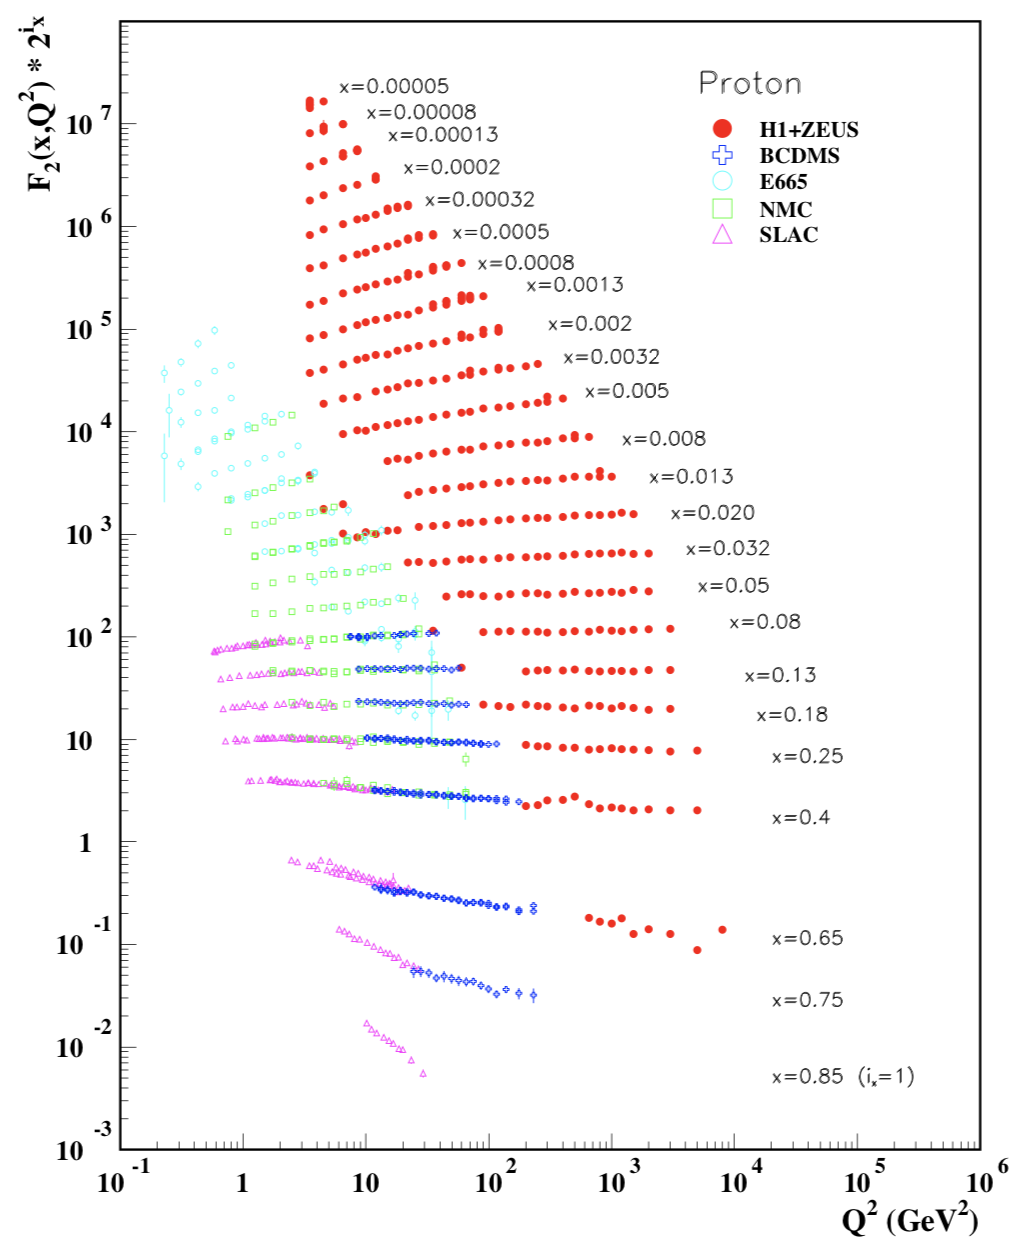
\includegraphics[scale=0.65]{./gfx/F2.png}
	\caption{The proton structure function $F^2_p$ measured in electromagnetic scattering of electrons and positrons on protons in the kinematic domain of the HERA data (collider experiments H$1$ and ZEUS for $Q^2 \geq 2$ GeV$^2$), and for electrons (SLAC) and muons (BCDMS, E$665$, NMC) on a fixed target. Figure taken from \cite{PDG}.}
	\label{pic:F2}
\end{figure}

\subsection{QCD-improved QPM}

The $Q^2$ dependence mentionned in previous subsection can be estimated by introducing quark interactions in the framework of QCD \cite{DISmeas,PICH}. Quantum ChromoDynamics is a non-abelian gauge theory based on a symmetry group SU($3$), which describes the interaction of quarks and gluons. The charge of this theory is called colour and the force carriers are the gluons, which are also coloured particles. The internal nucleon dynamic is due to the gluon emission and absorption and quark-antiquark pair creation from gluons. This creates a cloud of gluons and virtual $q\bar{q}$ pairs known as sea quarks.

The QCD coupling constant $\alpha_s$ depends on the scale of the interaction. At low energies quarks or gluons are always forming colorless particles, which are named hadrons : this is called confinement. At high energies quarks or gluons are free particles : this is asymptotic freedom.

Depending on the energy regime, a process can be labeled as a hard ($\alpha_s \sim 0$) or soft process ($\alpha_s large$). Hard processes can be described within the perturbative QCD (pQCD) framework, while soft processes can only be parametrized from experimental data. As in DIS the scale variable is often chosen as $Q^2$, the DIS cross-section is factorized \cite{CollinsSoper} in terms of soft and hard processes for $Q^2 > 1$ GeV$^2$, where $\alpha_s$ is small enough : the hard process is described by the lepton-quark cross-section $\sigma_q$ convoluted with the soft process parametrized by the PDFs. These two regimes differ by the factorisation scale $\Lambda$ that is mostly chosen as $Q^2$.

The resolution of the virtual photon probe is proportional to $1/Q^2$ (see Fig.~\ref{pic:Q2res} at fixed $x$). At $Q^2 \sim 0$, the virtual photon sees the nucleon as a point-like particle. As $Q^2$ increases, the virtual photon starts to resolve the nucleons constituents. At large $Q^2$ the virtual photon is able to resolve point-like quarks. The first QCD correction to the QPM concerns the gluon emission by the initial and the final quark.

\begin{figure}[!h]
  \centering
	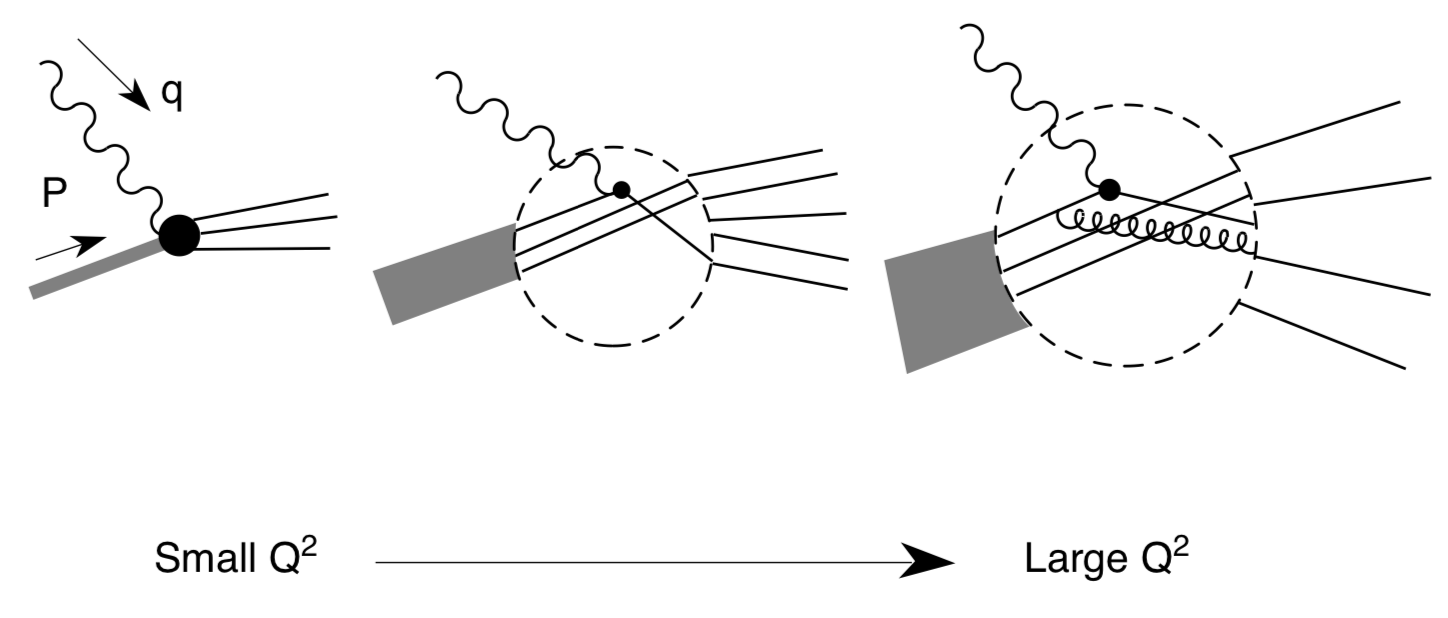
\includegraphics[scale=0.6]{./gfx/Q2res.png}
	\caption{Resolution of the photon probe versus $Q^2$. Figure taken from \cite{PICH}.}
	\label{pic:Q2res}
\end{figure}

The $Q^2$ dependence can be calculated using the Dokshiter-Gribov-Lipatov-Altarelli-Parisi (DGLAP) equations \cite{Dokshitser, GL1, GL2, AP} :
%
\begin{equation}
  \frac{dq_i(x,Q^2)}{dlnQ^2} = \frac{\alpha_s(Q^2)}{2\pi}\sum\limits_{j}\int_{x}^{1}P_{ij}(x/\xi,\alpha_s(Q^2))q_i(\xi,Q^2).
\end{equation}
%
Here, the splitting functions $P_{ij}(x/\xi)$ \cite{Joosten} are the probability that a quark or gluon of type $j$ and momentum fraction $\xi$ is the parent of $i$ with momentum fraction $x$. A similar equation holds for the gluon distribution. If the PDFs are known at a given scale $Q_0^2$, they can be evolved to any given $Q^2$ using these equations.

%----------------------------------------------------------------------------------------

\section{Determination of Parton Distribution Functions}

The PDFs are non-perturbative quantities and thus cannot be calculated from a theoretical framework. A global fit to world data is the only way to quantify them. It is possible to fit measurement coming from different processes because PDFs are universal quantities, i.e. they are process independent. The world data consists mostly of lepton-nucleon DIS but collider experiments ($pp$ or $p\bar{p}$) or neutrino scattering can be used for special contributions, e.g. for gluons or strange quarks. As experiments cover different kinematic ranges, this allows one to determine the PDFs in a large ($x$,$Q^2$) space.

For the fit to be performed, a functional form has to be provided at an initial scale $Q^2_0$. Often the form $xq_i(x,Q^2_0) = x^{\alpha}(1-x)^{\beta}$, where $q_i$ are partons, is used with additional terms refining the fit, reaching a number of free parameters from $10$ to $25$. The DGLAP equations are then used to evolve the PDFs to a given $Q^2$. An example of a fit done by the MMHT group \cite{MMHT} at Next to Leading Order (NLO) for different $Q^2$ values is shown in Fig.~\ref{fig:MMHT}.

\begin{figure}[htb!]
\centerline{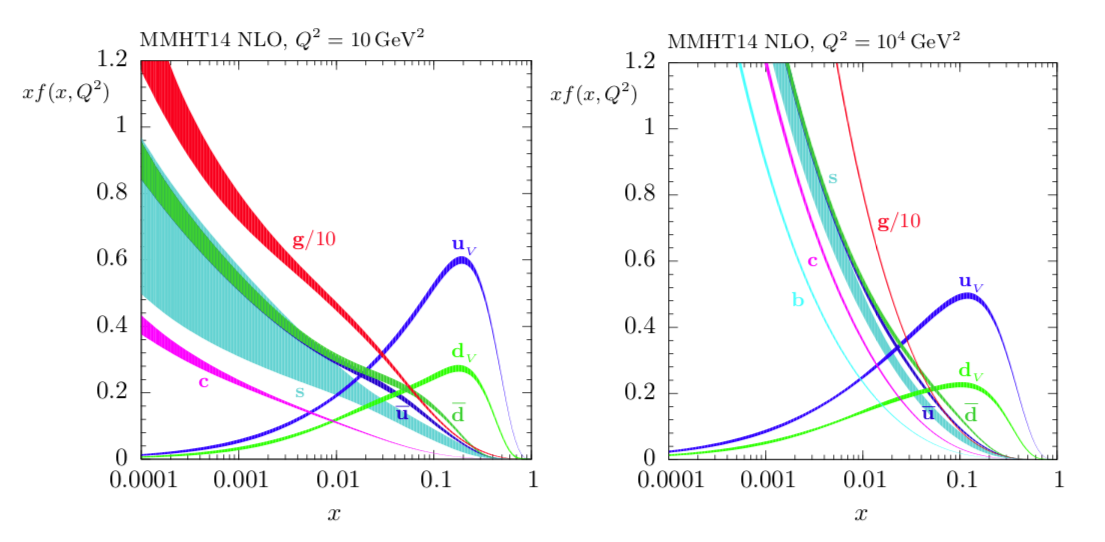
\epsfig{file=gfx/MMHT.png,width=14cm}}
\caption{Unpolarized PDFs at Next to Leading Order (NLO) from MMHT group at $Q^2$ = $10$ GeV$^2$ (left) and $Q^2$ = $10^4$ GeV$^2$ (right) with associated 68\% confidence-level uncertainty bands. Figure taken from \cite{MMHT}.}\label{fig:MMHT}
\end{figure}

%----------------------------------------------------------------------------------------

\section{Semi-Inclusive Deep Inelastic Scattering}

SIDIS is the semi-inclusive measurement of DIS. In the final state, at least one hadron and the scattered lepton are detected ($l+N \rightarrow l'+h+X$) and a new invariant variable $z$ is introduced, which corresponds to the energy fraction of the virtual photon held by the hadron $h$ :
%
\begin{equation}
  z = \frac{\textbf{P}\cdot\textbf{p}_h}{\textbf{P}\cdot\textbf{q}} \stackrel{lab}{=} \frac{E_h}{\nu}.
  \label{eq:SIDIS}
\end{equation}
%
The semi-inclusive cross section reads \cite{SIDISXS}:
%
\begin{equation}
  \frac{d\sigma}{dxdydz} = \frac{8\pi\alpha^2ME}{Q^4}\left[xy^2H_1(x,Q^2,z)+(1-y)H_2(x,Q^2,z)\right],
  \label{eq:SIDISXS}
\end{equation}
%
where $H_1$ and $H_2$ are structure functions related to $F_1$ and $F_2$ \cite{BERGER,SIDISXS} :
%
\begin{equation}
  \sum\limits_{h}\int_{0}^{1} H_i(x,Q^2,z)dz = F_i(x,Q^2)\quad,\quad i \in  \llbracket1,2\rrbracket.
\end{equation}
%
Additional variables used to describe the hadron kinematics are given in Table.~\ref{tab:SIDIS}.

\begin{table}[h!]
  \caption{SIDIS kinematic variables.}
  \label{tab:SIDIS}
  \begin{tabularx}{\textwidth}{r|lX}
    \hline
    \hline
    Variable & Description \\
    \hline
    \hline
    $\textbf{p}=(E_h,\vec{p}_h)$ & Hadron $4$-momentum vector \\
    $p_{h\|}$ & Component of $\vec{p}_h$ along $\vec{q}$ \\
    $p_{h\bot}$ & Transverse component of $\vec{p}_h$ with respect to $\vec{q}$ \\
    $\theta_h$ & Angle between $\vec{q}$ and $\vec{p}_h$ \\
    $\Phi_h$ & Angle between the scattering plane and the hadron production plane \\
    $z=\frac{E_h}{\nu}$ & Energy fraction of the virtual photon transferred to the hadron $h$ \\
    $\eta=\frac{1}{2}\text{ln}\left(\frac{|\mathbf{p}|+p_L}{|\mathbf{p}|-p_L} \right)$ & Pseudorapidity \\
    \hline
    \hline
  \end{tabularx}
\end{table}

\subsection{SIDIS in QPM}

The factorization Ansatz is also valid for SIDIS measurement thus the hadron production can be described as a convolution of three independent processes : the soft part $q(x)$ that are the PDFs, the hard process $\sigma_q$ describing the absorption of the virtual photon $\gamma^*$ by the quark $q$ and the soft part $D_q^h(z)$ characterize the fragmentation of the quark $q$ into a hadron $h$.

\begin{figure}[!h]
  \centering
	% 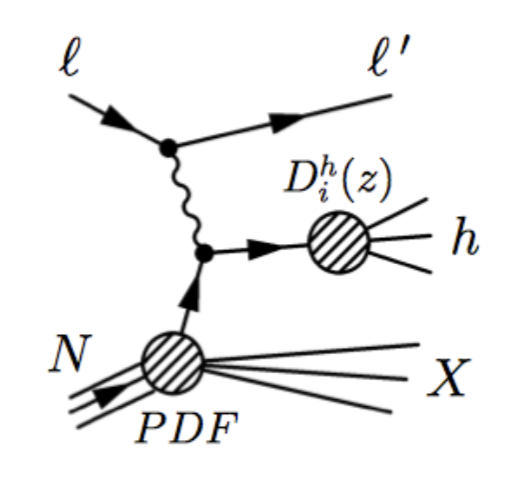
\includegraphics[scale=0.6]{./gfx/SIDIS.png}
  \begin{tikzpicture} \begin{feynman}
  \vertex (i1) {\(l\)};
  \vertex[right=2cm of i1] (a);
  \vertex[above right=2cm of a] (i2) {\(l'\)};
  \vertex[blob,below=2cm of a] (b) {\(\sigma_q\)};
  \vertex[blob,below left=2cm of b] (c) {\(q(x)\)};
  \vertex[below left=2cm of c] (f12) {\(N\)};
  \vertex[right=2cm of c] (f22);
  \vertex[below=0.3cm of f22] (f23);
  \vertex[above=0.3cm of f22] (f21);
  \vertex[blob, right=of b] (d) {\(D^h_q(z)\)};
  \vertex[above right=of d] (d1) {\(h^{\pm}\)};
  \vertex[right=of d] (d2) {\(\pi^{\pm}\)};
  \vertex[below right=of d] (d3) {\(K^{\pm}\)};

  \diagram* { (i1) -- [fermion] (a) -- [fermion] (i2),
  (a) -- [photon, edge label=\(\gamma^*\)] (b) [blob],
  (c) [blob] -- [fermion] (b) [blob],
  (b) [blob] -- [fermion] (d) [blob],
  (f12) -- [double distance=7pt] (c) [blob] -- [plain] (f22),
  (f12) -- [fermion] (c) [blob],
  (c) [blob] -- [plain] (f21),
  (c) [blob] -- [plain] (f23),
  (d) [blob] -- [plain] (d1),
  (d) [blob] -- [plain] (d2),
  (d) [blob] -- [plain] (d3),
  };
  \draw [decoration={brace}, decorate] (f21.north east) -- (f23.south east) node [pos=0.5, right] {\(X\)};
  \end{feynman} \end{tikzpicture}
	\caption{Factorization in SIDIS.}
	\label{pic:SIDIS}
\end{figure}

The structure functions $H_i(x,Q^2,z)$ contain the information on what happens to the struck quark after the interaction with the virtual photon. The fragmentation function (FF) $D_q^h(z,Q^2)$ is defined as the probability for a quark of flavour $q$ to fragment into a hadron $h$ with a fraction of energy $z$. The expression of the spin averaged SIDIS cross section can be expressed within QPM at LO in terms of PDFs and FFs \cite{BERGER,Panknin} :
%
\begin{equation}
  \frac{d^3 \sigma}{dxdydz} \stackrel{LO}{=} \frac{8\pi\alpha^2ME}{Q^2}\left[\frac{1}{2}y^2+\left(1-y-\frac{y^2 \gamma^2}{4}\right)\right]x\sum\limits_qe^2_qq(x)D_q^h(z).
  \label{eq:unpolSIDIS}
\end{equation}

%----------------------------------------------------------------------------------------

\section{Fragmentation Functions}\label{sec:FF}

When computing the cross-section of a given process $A+B \rightarrow h+X$, this cross-section is found to be a convolution of three different terms (Eq.~\ref{eq:facto}) : one non-perturbative term involving the PDFs (probability to obtain parton $a$ from nucleus $A$ $f_{a/A}(x_a,Q^2)$), one hard cross-section term for perturbative calculation ($d\sigma_{a,b \rightarrow c}(x_a,x_b,Q^2)$) and a last non-perturbative term involving the FFs (probability to obtain hadron $h$ from parton $c$ $D^h_c(x_c,Q^2)$).
%
\begin{equation}
  d\sigma_{A+B \rightarrow h+X} = \sum_{a,b,c} \left[ f_{a/A}(x_a,Q^2) f_{b/B}(x_b,Q^2) \right] \otimes \left[ d\sigma_{a,b \rightarrow c}(x_a,x_b,Q^2) \right] \otimes \left[ D^h_c(x_c,Q^2) \right]
  \label{eq:facto}
\end{equation}
%
Fig.~\ref{pic:SIDIS} illustrates this factorization in SIDIS. The extraction of FFs can also be done from electron-positron annihilation and hadron-hadron collisions measurements. The universality of FFs has been experimentally tested by Kniehl, Kramer and Pötter \cite{Universality}. Different ideas have been developed to model how quarks confine together to make a hadron.

\subsection{Lund String Fragmentation Model}

In the Lund String Model \cite{LUND}, the hadron production is explained by the creation of quark-antiquark pairs $q\bar{q}$. The strong interaction between partons is represented by a string. The energy inside the string is linear function of the distance between two stringed partons. At some point the energy is large enough to create a new $q\bar{q}$ pair and the string breaks. All unpaired remnants have new strings and the process repeats until there are only hadrons. The hadronization scheme in the Lund model in the center of mass frame is illustrated in Fig.~\ref{pic:Lund} (a). The virtual photon is absorbed e.g. by a $u$ quark and in consequence the $u$ quark is ejected from the nucleon. A new $q\bar{q}$ pair is created by the string breaking e.g. $d\bar{d}$. The remaining $u$ quark binds with the $\bar{d}$ quark to form a $\pi^+$ with a given $z$ as shown in Fig.~\ref{pic:Lund} (b). The remaining system repeats fragmentation process until the energy is smaller than the available energy $\nu$. In addition baryon creation by di-$q\bar{q}$ pair formation is introduced.

\begin{figure}[!h]
  \centering
	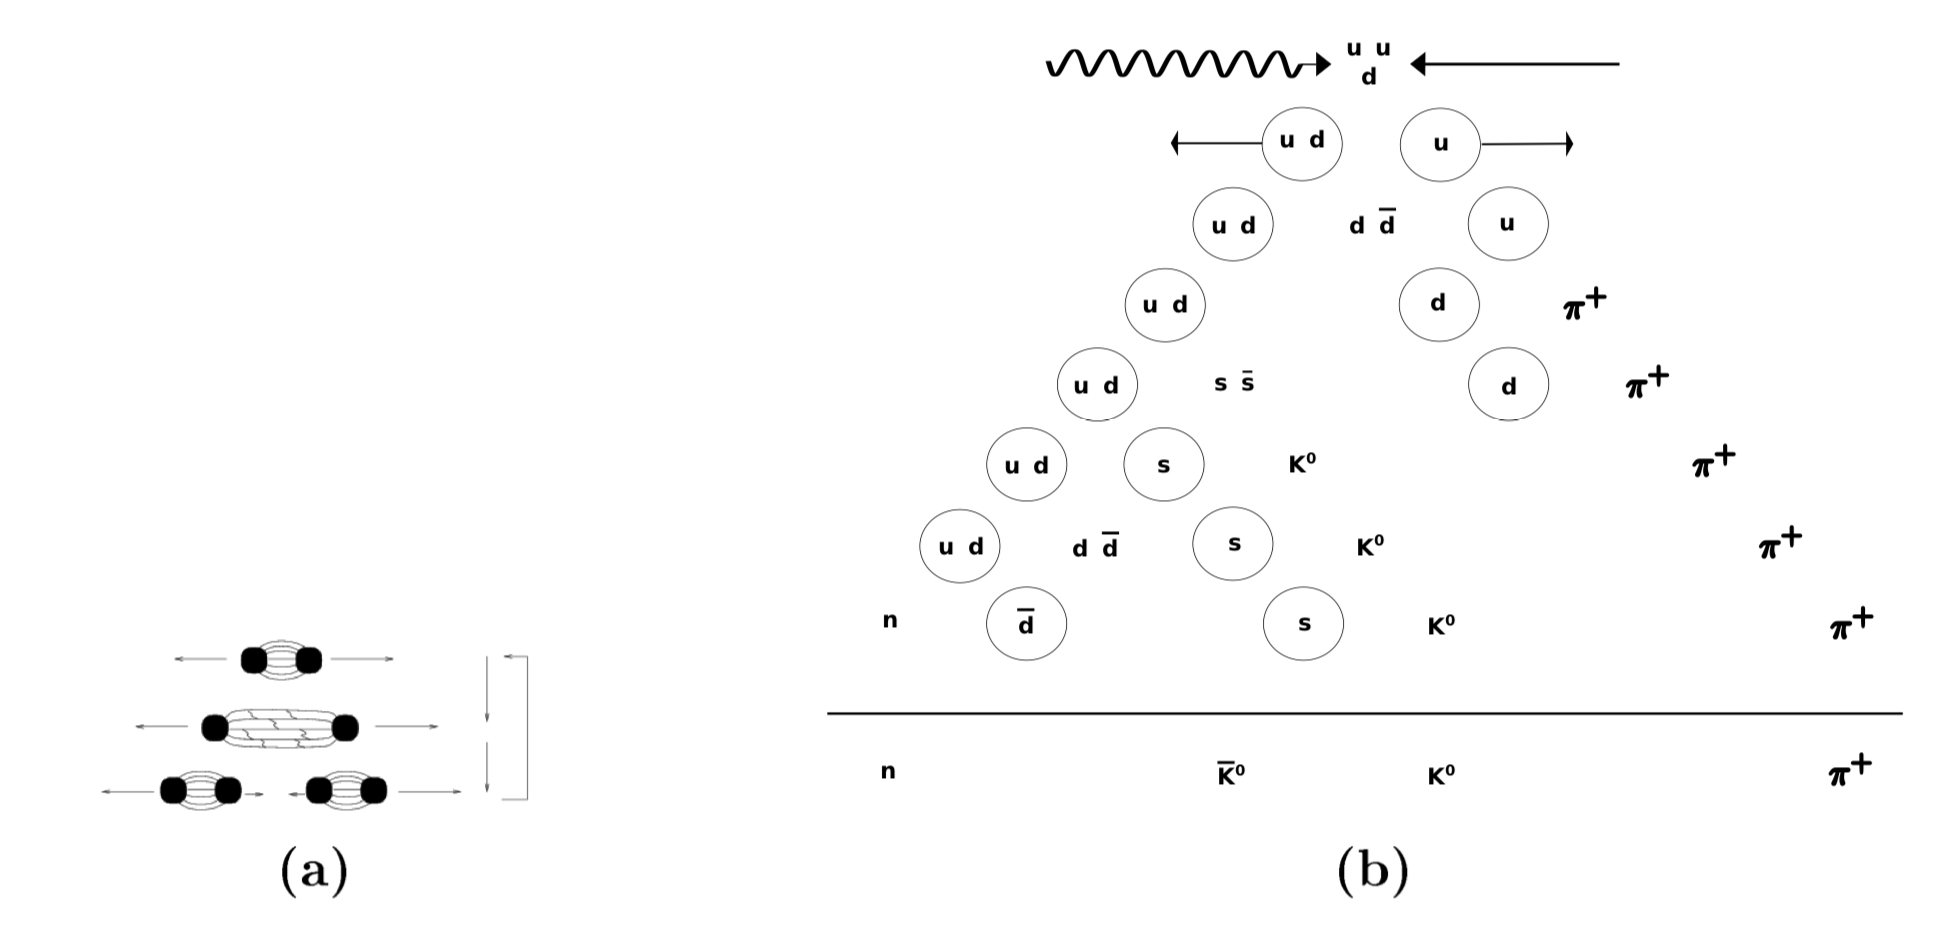
\includegraphics[scale=0.45]{./gfx/Lund.png}
	\caption{The fragmentation process in the Lund model. In (b), the produced $K^0$, $\overline{K^0}$, $\pi^+$ or $n$ could also be an excited state. Figure taken from \cite{Panknin}.}
	\label{pic:Lund}
\end{figure}

\subsection{Quark Fragmentation Regions}

Up to this point only the fragmentation of the struck quark was considered. The spectator quarks, which are not involved in the scattering process, have also to hadronize. This phenomenon is happening in two distinct $p_h$ regions : the target fragmentation region, where the final hadron $h$ has a small momentum in the rest frame of the target, and the current fragmentation region, where the product $\textbf{P}\cdot\textbf{p}_h$ grows with $Q^2$. At low energies there is a large overlap of these regions, while at high energies they start to separate. This hadron production can contaminate the SIDIS measurement of current fragmentation. To deal with this issue, Berger \cite{BERGER} came with a criterion based on the pseudorapidity of the final state $\eta$, which is the measurement of the longitudinal momentum. The sign of $\eta$ is linked to the different regions : if $\eta$ $>$ $0$ the hadron moves towards the direction of the virtual photon and is a current hadron, else is $\eta$ $<$ $0$ the hadron is a target remnant (Fig.~\ref{pic:Berger}). Defining $p(k)$ to be the probability that $k$ hadrons of some specific type decay from one cluster, one finds that the \textit{fully inclusive} correlation function has the form :
%
\begin{equation}
  C(y_1,y_2) = \frac{\langle k(k-1) \rangle}{\langle k \rangle} \left(\frac{1}{\sigma}\frac{d\sigma}{dy}\right)_{y\sim 0} G(y_1-y_2),
\end{equation}
%
when $y_1$ and $y_2$ are in the central region and the averages are :
%
\begin{equation}
  \begin{split}
    \langle k \rangle = \sum kp(k) \\
    \langle k-1 \rangle = \sum k(k-1)p(k).
  \end{split}
\end{equation}
%
The Gaussian function :
%
\begin{equation}
  G(y_1-y_2) = \frac{1}{2\delta \sqrt{\pi}}exp\left[-\frac{\left(y_1-y_2\right)}{4\delta^2}\right],
\end{equation}
%
has an effective \textit{correlation length} of $2\delta$. As the typical hadronic correlation length in pseudorapidity is $\delta \sim 2$, a separation criterion, the Berger criterion, is that $\Delta\eta = \eta_{max}-\eta_{min} \geq 2\delta$ or in terms of DIS kinematics variables $W \gtrsim 7.4$ GeV. It is important to select the kinematic region so that selected hadrons are dominated by the struck quark fragmentation.

\begin{figure}[!h]
  \centering
	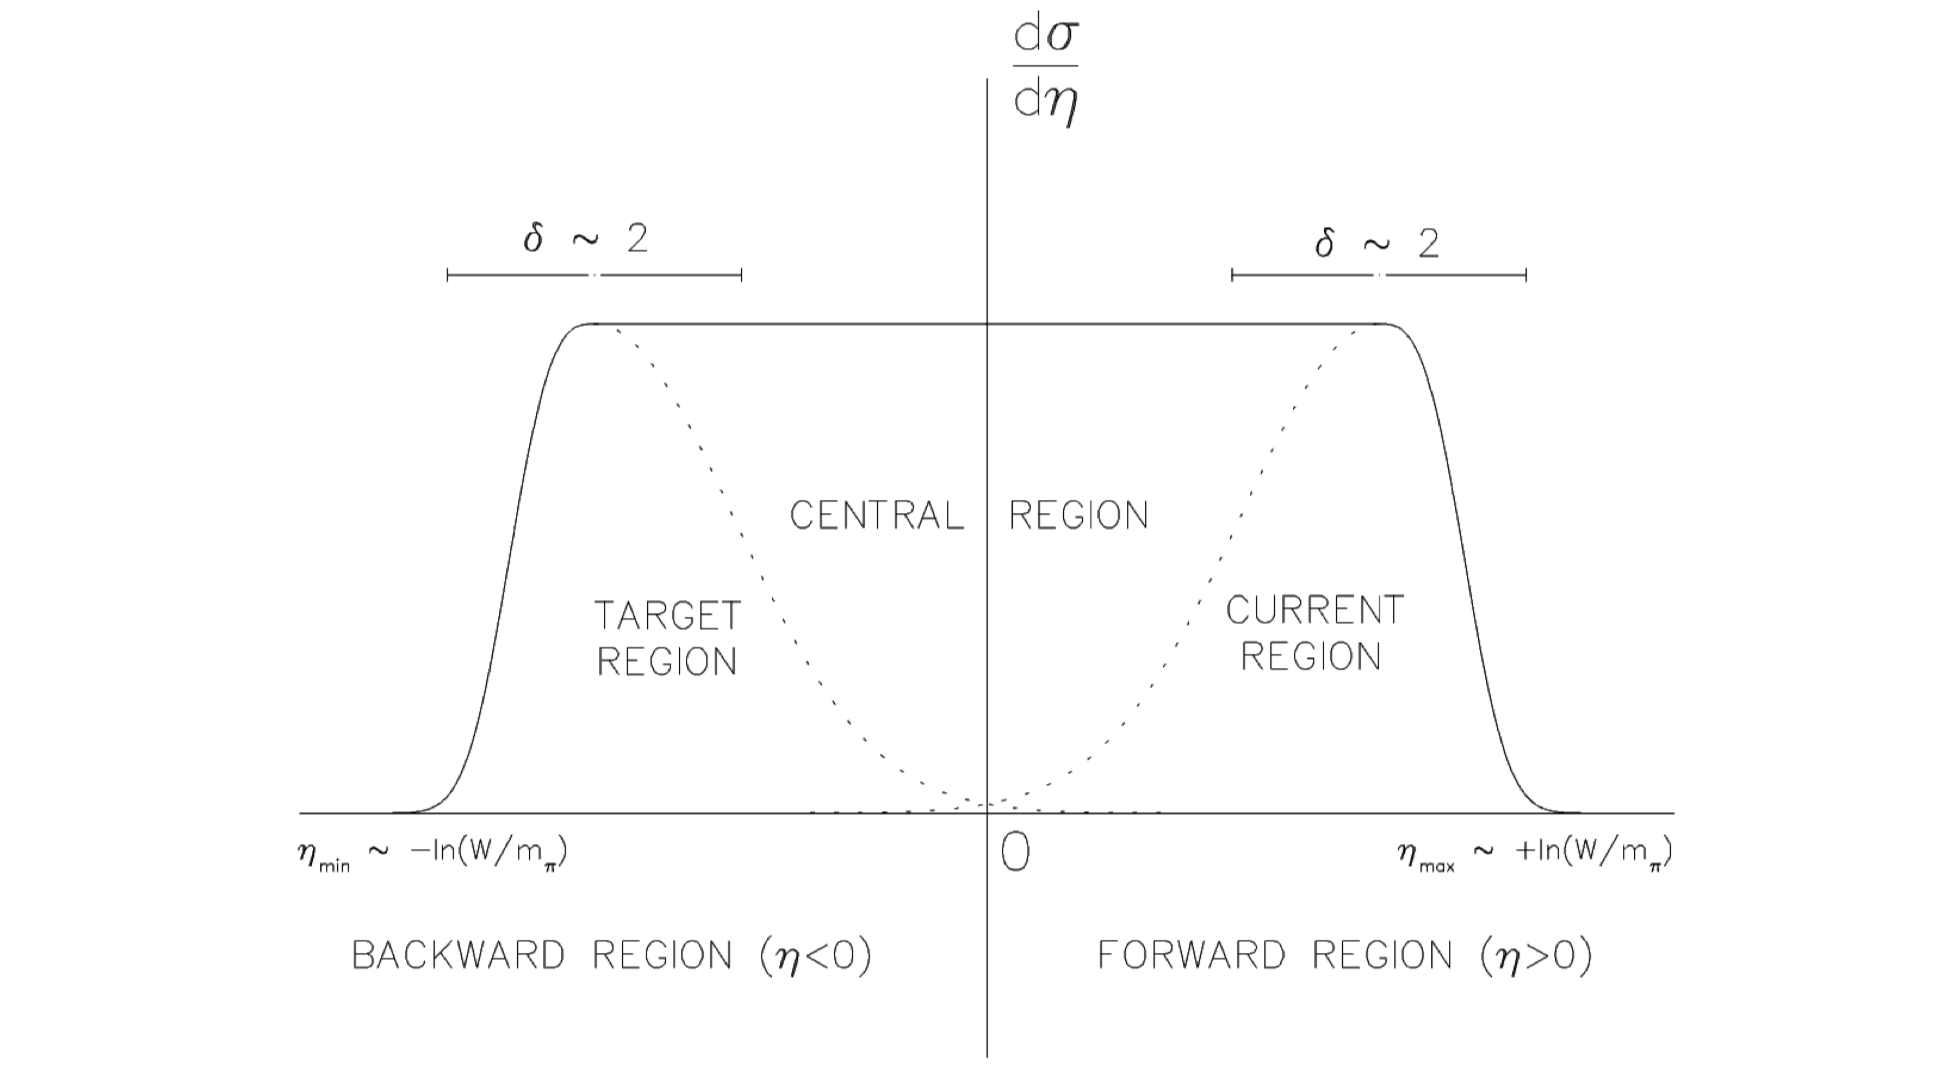
\includegraphics[scale=0.5]{./gfx/Berger.png}
	\caption{Hadronic pseudorapidity ($\eta$) distribution at very high energies. Figure taken from \cite{Niczy}.}
	\label{pic:Berger}
\end{figure}

\subsection{Scaling and $Q^2$ evolution}

For the FFs extracted from $e^+e^-$ annihilation displayed in Fig.~\ref{pic:FFscale}, the scaling is present for a wide $x = 2p_h/\sqrt{s}$ range (Fig.~\ref{pic:FFscale} (a)). At low x ($x$ $<$ $0.1$) the FFs increases with the total center-of-mass energy $\sqrt{s}$ (Fig.~\ref{pic:FFscale} (b)), while at large $x$, the FFs are shifted towards lower values for large $Q^2$ (similar behaviour as PDFs). Here $\sqrt{s}$ has the same role has $Q^2$. Scaling violation is observed \cite{PDG}.

\begin{figure}[!h]
  \centering
	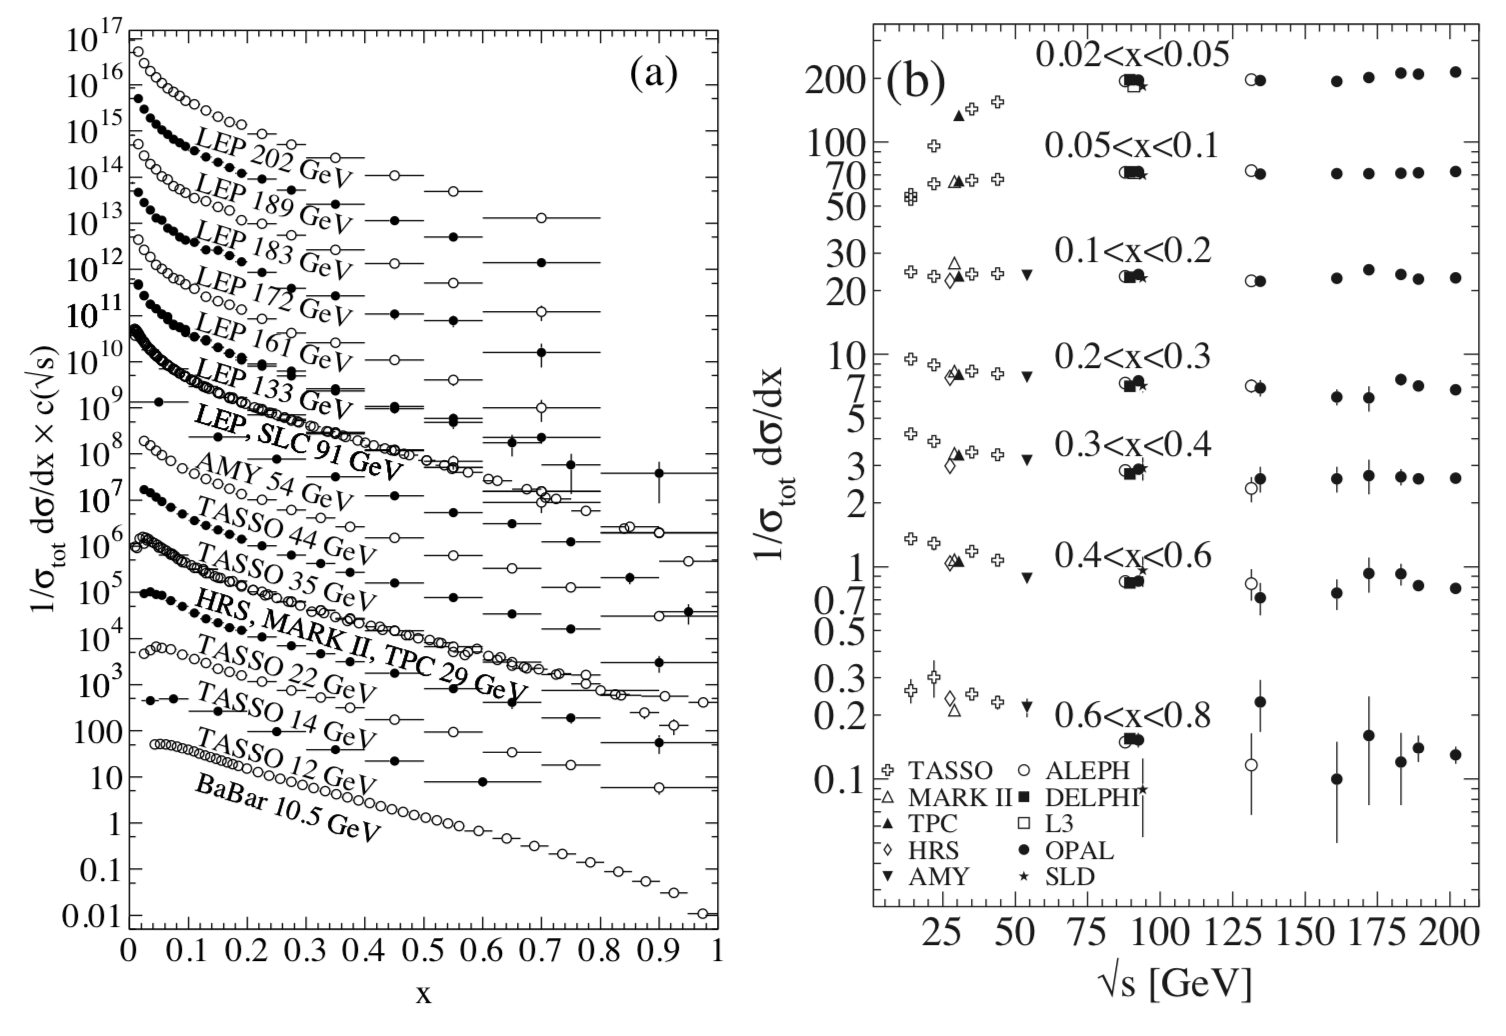
\includegraphics[scale=0.6]{./gfx/FFscale.png}
	\caption{The $e^+ e^-$ fragmentation function for all charged particles for different center of mass energy $\sqrt{s}$ versus $x$ (a) and for various range of $x$ versus $\sqrt{s}$ (b). Figures taken from \cite{PDG}.}
	\label{pic:FFscale}
\end{figure}

The evolution of the fragmentation functions is also described by DGLAP equations \cite{Dokshitser, GL1, GL2, AP} :
%
\begin{equation}
  \frac{dD_q^h(z,Q^2)}{dlnQ^2} = \frac{\alpha_s(Q^2)}{2\pi}\sum\limits_j\int_{x}^{1}P_{qj}\left(z/\xi,\alpha_s(Q^2)\right)D_q^h(\xi,Q^2)\frac{d\xi}{\xi}.
\end{equation}
%
In Fig.~\ref{pic:QuarkFrag} the process contributing to the $Q^2$-evolution is illustrated~: the fragmentation of a quark $q_i$ through its own hadronization after emmiting a gluon $G$ ($P_{qq}D_{q_i}^h$), through the hadronization of a gluon $G$ ($P_{Gq}D_{G}^h$), the fragmentation of a gluon splitting into a quark-antiquark pair and following hadronization of the quark in hadron ($P_{qG}D_{q_i}^h$) and eventually the gluon fragmentation via the three-gluon self-interaction ($P_{GG}D_{G}^h$).

\begin{figure}[!h]
  \centering
	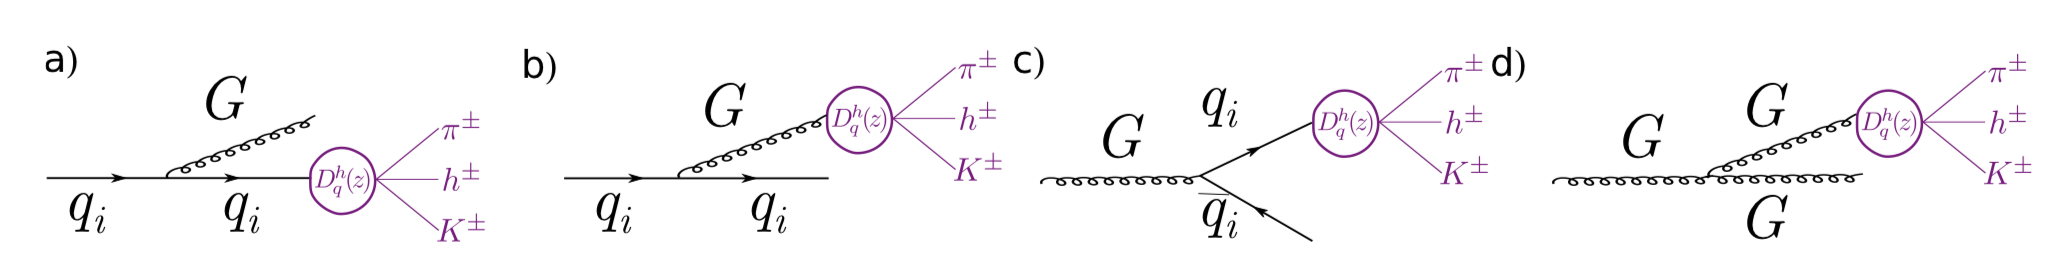
\includegraphics[scale=0.45]{./gfx/QuarkFrag.png}
	\caption{The fragmentation of the quark $q_i$ decaying into a hadron $h$ while emitting a gluon $G$ ($P_{qq}D^h_{q_{i}}$) (a), the fragmentation of the quark $q_i$ through a gluon $G$ ($P_{Gq}D^h_{G}$) (b), the fragmentation of the gluon $G$ via the creation of a $q_i \bar{q_i}$ pair and the decay of $q_i$ ($P_{qG}D^h_{q_{i}}$) (c) and the fragmentation of the gluon $G$ via a three gluon vertex ($P_{GG}D^h_{G}$) (d). Figure taken from \cite{Uematsu}.}
	\label{pic:QuarkFrag}
\end{figure}

\subsection{Fragmentation Function Symmetries}

One FF $D^h_q(z,Q^2)$ is introduced for each flavour $q$ and each hadron species $h$. Considering only the light quarks ($u$,$\bar{u}$,$d$,$\bar{d}$,$s$ and $\bar{s}$), in case the mass threshold for heavy quarks is higher than the covered kinematic domain, implies that for charged hadrons one has to measure twelve different fragmentation functions for positive and negative hadrons. Nevertheless, within the QCD-improved QPM, symmetries as isospin or charge-conjugation can be used to reduce the number of independent fragmentation functions.

The FFs can be split into two main categories. If a quark fragments into a hadron h and the quark is a valence quark of $h$, the FF is said to be favoured ($D^h_{fav}$). If it is a sea quark of $h$, the FF is unfavoured ($D^h_{unf}$).

For pions charge-conjugation symmetry reduces the number of independent fragmentation functions to six. The application of the isospin (viz. $D^{\pi^+}_u = D^{\pi^+}_{\bar{d}}$ for $\pi^+$) and SU($3$) symmetries lowers this number further to two :
%
\begin{equation}\label{eq:FFPion}
  \begin{split}
    D^h_{fav} : D^{\pi^+}_u = D^{\pi^-}_{\bar{u}} = D^{\pi^-}_d = D^{\pi^+}_{\bar{d}}, \\
    D^h_{unf} : D^{\pi^-}_u = D^{\pi^+}_{\bar{u}} = D^{\pi^+}_d = D^{\pi^-}_{\bar{d}} \stackrel{SU(3)\,sym.}{=} D^{\pi^{\pm}}_s = D^{\pi^{\mp}}_{\bar{s}}.
  \end{split}
\end{equation}

For kaons charge-conjugation symmetry reduces the number of independent fragmentation functions to six. The application of the isospin (viz. $D^{\pi^+}_u = D^{\pi^+}_{\bar{d}}$ for $\pi^+$) and SU($3$) symmetries lower the number to three independent FFs : the favoured, grouping the kaons valence quarks $u$ and $\bar{u}$ FFs, the strange, grouping the kaons valence quarks $s$ and $\bar{s}$ FFs and the unfavoured, grouping the kaons sea quark FFs :
%
\begin{equation}\label{eq:FFKaon}
  \begin{split}
    D^h_{fav} : D^{K^+}_u = D^{K^-}_{\bar{u}} \\
    D^h_{str} : D^{K^+}_{\bar{s}} = D^{K^-}_{s} \\
    D^h_{unf} : D^{K^+}_{\bar{u}} = D^{K^-}_{u} = D^{K^+}_s = D^{K^-}_{\bar{s}} = D^{K^{\pm}}_{d} = D^{K^{\mp}}_{\bar{d}}
  \end{split}
\end{equation}

%----------------------------------------------------------------------------------------

\section{State of the art of the fragmentation functions}

\subsection{Measurements}

The production of hadrons from the the struck quark cannot be computed as final state hadron masses are of order or smaller than $\Lambda_{QCD}$. In order to extract FFs reliably from the $Q^2$ dependence of the measured hadron production, a large kinematic range is needed. Thus data taken at different energies are used. Three different processes are so far used to extract quark fragmentation functions : electron-positron annihilation (SIA), lepton-nucleon (SIDIS) and hadron-hadron collisions ($pp$ or $p\bar{p}$). A summary of the aspects of the different processes can be found in Table.~\ref{tab:FFProcesses}. The SIA data (LEP \cite{LEP1,LEP2,LEP3}, SLAC \cite{SLAC1}, BaBar \cite{BABAR} and BELLE \cite{BELLE}) provide the cleanest access to the FFs, since the cross-section of the process does not involve PDFs and are well calculated up to NNLO. But due to the dependence of the cross-section on $e^2_q$, $D^h_q$ and $D^h_{\bar{q}}$ cannot be separated and there is a limited access to gluon FF $D^h_g$. The data from hadron-hadron collisions (UA5 \cite{UA5}, UA1 \cite{UA1}, ALICE \cite{ALICE}, CMS \cite{CMS1,CMS2}, ATLAS \cite{ATLAS}, RHIC \cite{RHIC1,RHIC2,RHIC3}) give access to $D^h_q$, $D^h_{\bar{q}}$ and $D^h_g$, but allow no direct access to $z$.

Data from SIDIS can be compared to data from previously presented processes for the current fragmentation region (see Section~\ref{sec:FF}). SIDIS data have the advantage that factorization has been proven to all orders of $\alpha_s$. In addition they cover a wide range in $Q^2$ in a single measurement compared to SIA. The experiments providing inputs for the SIDIS process are EMC \cite{EMC} and COMPASS \cite{COMPASS2006Pi,COMPASS2006K} using muon beam and E$00$-$108$ \cite{E00108} and HERMES \cite{HERMESMult} using electron beam. All experiments measured with proton and deuteron targets.

\begin{table}[!h]
  \caption{Fragmentation functions access for different processes.}
  \label{tab:FFProcesses}
  \centering
  \begin{tabular}{cccc}
    \hline
    \hline
    & $e^+ e^- annihilation$ & $pp$/$p\bar{p}$ collision & DIS \\
    \hline
     &   \resizebox{3cm}{3.5cm}{\begin{tikzpicture} \begin{feynman}
     \vertex (i1) {\(e^{-}\)};
     \vertex[right=2cm of i1] (a);
     \vertex[above right=2cm of a] (i2) {\(e^{+}\)};
     \vertex[blob,below=2cm of a] (b) {\(\widehat{\sigma_q}\)};
     \vertex[below left=2cm of b] (f12);
     \vertex[below=0.3cm of f12] (f13);
     \vertex[above=0.3cm of f12] (f11);
     \vertex[blob,below right=2cm of b] (d) {\(D^h_q(z)\)};
     \vertex[above right=of d] (d1) {\(h^{\pm}\)};
     \vertex[right=of d] (d2) {\(\pi^{\pm}\)};
     \vertex[below right=of d] (d3) {\(K^{\pm}\)};

     \diagram* { (i1) -- [fermion] (a) -- [anti fermion] (i2),
     (a) -- [photon, edge label=\(\gamma^{*}/Z^{0}\)] (b) [blob],
     (f12) -- [plain] (b) [blob] -- [fermion] (d) [blob],
     (f13) -- [plain] (b) [blob],
     (f11) -- [plain] (b) [blob],
     (d) [blob] -- [plain] (d1),
     (d) [blob] -- [plain] (d2),
     (d) [blob] -- [plain] (d3),
     };
     \draw [decoration={brace}, decorate] (f13.south west) -- (f11.north west) node [pos=0.5, left] {\(X\)};
   \end{feynman} \end{tikzpicture}}
      & \resizebox{3.5cm}{3cm}{\begin{tikzpicture} \begin{feynman}
    \vertex (i1) {\(p\)};
    \vertex[blob,right=2cm of i1] (a) {\(q(x)\)};
    \vertex[below=6cm of i1] (i2) {\(p/\bar{p}\)};
    \vertex[blob,right=2cm of i2] (b) {\(q(x)\)};
    \vertex[blob,below right=4cm of a] (c) {\(\widehat{\sigma}_q\)};
    \vertex[above right=of c] (f1);
    \vertex[blob, below right=of c] (d) {\(D^h_q(z)\)};
    \vertex[above right=of d] (d1) {\(h^{\pm}\)};
    \vertex[right=of d] (d2) {\(\pi^{\pm}\)};
    \vertex[below right=of d] (d3) {\(K^{\pm}\)};

    \diagram* { (i1) -- [double distance=7pt] (a) [blob], (i1) -- [fermion] (a) [blob],
    (i2) -- [double distance=7pt] (b) [blob], (i2) -- [fermion] (b) [blob],
    (a) -- [fermion] (c) [blob], (b) -- [fermion] (c) [blob], (c) [blob] -- [fermion] (f1), (c) [blob] -- [fermion, edge label=\(q\)] (d) [blob],
    (d) [blob] -- [plain] (d1),
    (d) [blob] -- [plain] (d2),
    (d) [blob] -- [plain] (d3),
    };
    \end{feynman} \end{tikzpicture}}
      & \resizebox{3cm}{3.5cm}{\begin{tikzpicture} \begin{feynman}
      \vertex (i1) {\(l\)};
      \vertex[right=2cm of i1] (a);
      \vertex[above right=2cm of a] (i2) {\(l'\)};
      \vertex[blob,below=2cm of a] (b) {\(\widehat{\sigma}_q\)};
      \vertex[blob,below left=2cm of b] (c) {\(q(x)\)};
      \vertex[below left=2cm of c] (f12) {\(N\)};
      \vertex[right=2cm of c] (f22);
      \vertex[below=0.3cm of f22] (f23);
      \vertex[above=0.3cm of f22] (f21);
      \vertex[blob, right=of b] (d) {\(D^h_q(z)\)};
      \vertex[above right=of d] (d1) {\(h^{\pm}\)};
      \vertex[right=of d] (d2) {\(\pi^{\pm}\)};
      \vertex[below right=of d] (d3) {\(K^{\pm}\)};

      \diagram* { (i1) -- [fermion] (a) -- [fermion] (i2),
      (a) -- [photon, edge label=\(\gamma^*\)] (b) [blob],
      (c) [blob] -- [fermion] (b) [blob],
      (b) [blob] -- [fermion] (d) [blob],
      (f12) -- [double distance=7pt] (c) [blob] -- [plain] (f22),
      (f12) -- [fermion] (c) [blob],
      (c) [blob] -- [plain] (f21),
      (c) [blob] -- [plain] (f23),
      (d) [blob] -- [plain] (d1),
      (d) [blob] -- [plain] (d2),
      (d) [blob] -- [plain] (d3),
      };
      \draw [decoration={brace}, decorate] (f21.north east) -- (f23.south east) node [pos=0.5, right] {\(X\)};
    \end{feynman} \end{tikzpicture}}\\
    Dependence & $\widehat{\sigma} \otimes FF$ & $\widehat{\sigma} \otimes PDF \otimes PDF \otimes FF$ & $\widehat{\sigma} \otimes PDF \otimes FF$ \\
    Separate $D^h_{q}$ / $D^h_{\bar{q}}$ & \ding{55} & \ding{51} & \ding{51} \\
    Access parton kinematics & \ding{51} & \ding{55} & \ding{51} \\
    Theoretical calculation & LO, NLO, NNLO & LO, NLO & LO, NLO \\
    \hline
  \end{tabular}
\end{table}

\subsection{Accessing the fragmentation functions in SIDIS}

Hadron multiplicities are defined as the cross-section ratio :
%
\begin{equation}
  M^h(x,Q^2,z) = \frac{d\sigma^{lN \rightarrow l'hX}}{d\sigma^{lN \rightarrow l'X}dz} = \frac{d\sigma^h(x,Q^2,z)/dxdQ^2dz}{d\sigma^{DIS}(x,Q^2)/dxdQ^2},
\end{equation}
%
equivalent to the number of hadrons produced per DIS events allowing to access FFs by measuring hadron multiplicities.

Using the expressions of the DIS and SIDIS cross-sections (Eqs.~\ref{eq:unpolDIS} and \ref{eq:unpolSIDIS}) one obtains in the QPM :
%
\begin{equation}\label{eq:MFFPDF}
  M^h(x,Q^2,z) = \frac{\sum_q e^2_q q(x,Q^2) \otimes D^h_q(z,Q^2)}{\sum_q e^2_q q(x,Q^2)} \stackrel{LO}{=} \frac{\sum_q e^2_q q(x,Q^2) D^h_q(z,Q^2)}{\sum_q e^2_q q(x,Q^2)}.
\end{equation}
%
As PDFs and FFs depend on different variables $x$ and $z$ one can write the convolution as a single product. By measuring $M^h(x,Q^2,z)$ for positive and negative hadrons, one can distinguish $D^h_q$ and $D^h_{\bar{q}}$. The procedure of FFs extraction from COMPASS multiplicity measurement is described in Chapter~\ref{ch:FF}.

\subsection{Global fits of multiplicity data and parametrizations of FFs}

As the FFs are universal quantities, a global QCD fit of available data on multiplicities from SIA, SIDIS and $pp$/$p\bar{p}$ collisions can be performed to give a general parametrization of the FFs. There are different parametrization available in the literature. Some parametrizations are only based on SIA data : KKP \cite{Universality}, KRE \cite{KRE} and HKNS \cite{HKNS}, when the AKK \cite{AKK} parametrization uses in addition some hadron-hadron scattering data. One only uses SIDIS data : LSS \cite{LSS}. The newest parametrizations from DSEHS \cite{DSEHS1,DSEHS2} include all three types of data and JAM \cite{JAM} parametrizations include SIA+SIDIS. Each parametrization has its own set of assumptions based on symmetries and its different parametrization of $D^h_q$. A summary of the assumptions of the different groups can be found in Table \ref{tab:FFParametrization}. Only DSEHS and JAM will be described in more details in the following as they are the latest ones (or have been updated recently).

\begin{table}[!h]
  \caption{Parametrization of FFs for pions and kaons.}
  \label{tab:FFParametrization}
  \centering
  \begin{tabular}{ccccccc}
    \hline
    \hline
    Parametrization & Year & \multicolumn{3}{c}{Data} & \multicolumn{2}{c}{\# FFs fitted} \\
    \hline
     & & SIDIS & $pp$/$p\bar{p}$ & SIA & $\pi$ & $K$ \\
    KKP \cite{Universality} & 2000 & \ding{55} & \ding{55} & \ding{51} & 5 & 5 \\
    KRE \cite{KRE} & 2001 & \ding{51} & \ding{55} & \ding{51} & 2 & 3 \\
    HKNS \cite{HKNS} & 2007 & \ding{55} & \ding{55} & \ding{51} & 2 & 2 \\
    AKK \cite{AKK} & 2008 & \ding{55} & \ding{51} & \ding{51} & 3 & 5 \\
    LSS \cite{LSS} & 2014 & \ding{51} & \ding{55} & \ding{55} & 3 & 3 \\
    DSEHS \cite{DSEHS1,DSEHS2} & 2017 & \ding{51} & \ding{51} & \ding{51} & 4 & 4 \\
    JAM \cite{JAM} & 2018 & \ding{51} & \ding{55} & \ding{51} & 3 & 3 \\
    \hline
  \end{tabular}
\end{table}

\subsubsection*{DSEHS parametrization}

DSEHS (previously DSS) was the first group, who determined individual FFs for quarks and antiquarks and the first to try to fit data coming from three different processes alltogether.
The functional form they use for $D^h_q$ is the following :
%
\begin{equation}
  D^h_i (z,Q_0) = \frac{N^h_i z^{\alpha^h_i}(1-z)^{\beta^h_i}\left[ 1+\gamma^h_i(1-z)^{\delta^h_i}\right]}{B\left[2+\alpha^h_i,1+\beta^h_i\right]+\gamma^h_i B\left[2+\alpha^h_i,1+\beta^h_i+\delta^h_i\right]},
  \label{eq:DSEHSparam}
\end{equation}
%
where $N^h_i$, $\alpha^h_i$, $\beta^h_i$, $\gamma^h_i$ and $\delta^h_i$  are the fit parameters and B is the Euler beta function. For pions the two independent favoured FFs are related by a proportionality factor $k$. Moreover, isospin symmetry is considered only for the unfavoured FF ($D^{\pi^{+}}_{\bar{u}} = D^{\pi^{+}}_{d}$) and the fragmentation of a strange quark into pion is related to the unfavoured FFs with $z$-dependent factor ($D^{\pi^{+}}_{\bar{s}} = D^{\pi^{+}}_{s}=N_s z^{\alpha_s} D^{\pi^{+}}_{\bar{u}}$). Thus four FFs are fitted for pions : $u+\bar{u}$, $d=\bar{u}$, $s+\bar{s}$ and $g$. For kaons, $D^{K^+}_{u+\bar{u}}$ and $D^{K^+}_{s+\bar{s}}$ are fitted independently to account for the fact that phenomenologically it is expected that the formation of secondary $s\bar{s}$, required to form $K^+$ from a $u$, should be suppressed. Previous fits from DSS showed that $D^{K^+}_{s+\bar{s}} > D^{K^+}_{u+\bar{u}}$, highlighting this fact. For the unfavoured FFs all distributions have the same functional form  $D^{K^+}_{\bar{u}} = D^{K^+}_{s} = D^{K^+}_{d} = D^{K^+}_{\bar{d}}$ as the data are unable to discrimate between flavours. Four FFs are fitted for kaons, as for the pions :  $u+\bar{u}$, $s+\bar{s}$ , $\bar{u}=d=\bar{d}=s$ and $g$.
The FFs for heavy quarks (c,b) are also considered above their $\overline{MS}$ mass thresholds.
The parameters are determined from a standard $\chi^2$ minimization :
%
\begin{equation}
  \chi^2 =  \sum_{i=1}^{m} \left[ \left( \frac{1-\mathscr{N}_i}{\delta\mathscr{N_i}} \right) + \sum_{j=1}^{m_i} \frac{(\mathscr{N}_i T_j - E_j)^2}{\delta E^2_j} \right],
  \label{eq:DSEHSmin}
\end{equation}
%
where $m$ is the number of datasets with $m_i$ points each, $E_j$ are the data points and $\delta E_j$ their error and $T_j$ the theoretical estimate for a given set. The normalisation factor $\mathscr{N}_i$ is defined as $\delta \chi^2 / \delta\mathscr{N}_i = 0$.

\begin{table}[!h]
  \caption{DSEHS FFs hypotheses for pions and kaons.}
  \label{tab:DSEHSParametrization}
  \centering
  \begin{tabular}{ll}
    \hline
    \hline
     & Pions \\
    \hline
    Favoured & $D^{\pi^{+}}_{u} = N_{\pi^{+}} D^{\pi^{+}}_{\bar{d}}$ = $D^{\pi^{-}}_{d} = k_{\pi^{-}} D^{\pi^{-}}_{\bar{u}}$ \\
    Unfavoured & $D^{\pi^{+}}_{\bar{u}} = D^{\pi^{+}}_{d}$ \\
    Unfavoured strange & $D^{\pi^{+}}_{\bar{s}} = D^{\pi^{+}}_{s}$ \\
     & $D^{\pi^{-}}_{\bar{d}} = D^{\pi^{-}}_{u}$ = $D^{\pi^{-}}_{\bar{s}} = D^{\pi^{-}}_{s} = k_{\pi^{-}} D^{\pi^{-}}_{u}$ \\
    Gluons & $D^{\pi^{+}}_{g} = D^{\pi^{-}}_{g}$ \\
    \hline
    \hline
     & Kaons \\
    \hline
    Favoured & $D^{K^{+}}_{u}, D^{K^{-}}_{\bar{u}}$ \\
    Unfavoured & $D^{K^{+}}_{\bar{u}} = D^{K^{+}}_{d} = D^{K^{+}}_{\bar{d}} = D^{K^{+}}_{s}$ \\
               & $D^{K^{-}}_{u} = D^{K^{-}}_{d} = D^{K^{-}}_{\bar{d}} = D^{K^{-}}_{\bar{s}}$ \\
    Strange & $D^{K^{+}}_{\bar{s}}, D^{K^{-}}_{s}$ \\
    Gluons & $D^{K^{+}}_{g}, D^{K^{-}}_{g}$ \\
  \end{tabular}
\end{table}

The favoured, unfavoured and gluon FFs from DSS at LO for $Q^2$ = 10 GeV$^2$ are shown as function of $z$ for $\pi^+$ in Fig.~\ref{pic:DSEHSPi} and $K^+$ in Fig.~\ref{pic:DSEHSK}.

\begin{figure}[!h]
  \centering
	\includegraphics[scale=0.47]{./gfx/DSEHSPi.png}
	\caption{Individual FFs for positively charged pions $zD^{\pi^+}(z,Q^2)$ at $Q^2$ = $10$ GeV$^2$ (solid lines) along with uncertainty estimates at $68$\% and $90$\% C.L. indicated by the inner and outer shaded bands, respectively. The panels on the right-hand-side show the corresponding relative uncertainties. Also shown is a comparison to previous DSS$07$ global analysis \cite{DSS07} (dashed lines). Figure taken from \cite{DSEHS1}.}
	\label{pic:DSEHSPi}
\end{figure}

\begin{figure}[!h]
  \centering
	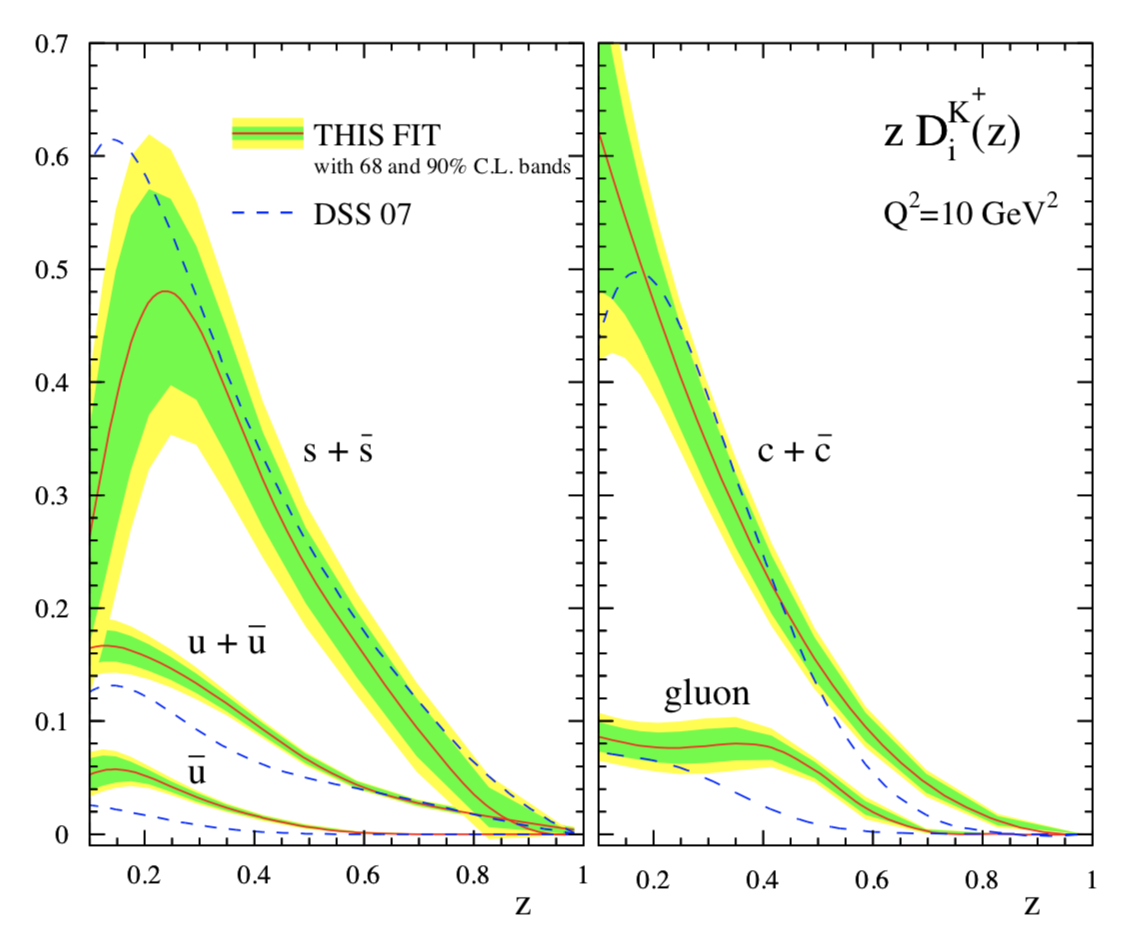
\includegraphics[scale=0.5]{./gfx/DSEHSK.png}
	\caption{Individual FFs for positively charged kaons $zD^{K^+}(z,Q^2)$ at $Q^2$ = $10$ GeV$^2$ (solid lines) along with uncertainty estimates at $68$\% and $90$\% C.L. indicated by the inner and outer shaded bands, respectively. Also shown is a comparison to previous DSS$07$ global analysis \cite{DSS07} (dashed lines). Figure taken from \cite{DSEHS2}.}
	\label{pic:DSEHSK}
\end{figure}

\subsubsection*{JAM parametrization}

JAM is a Monte-Carlo based combined fit of PDFs and FFs using Bayesian statistics. In order to address some of the questions raised by the recent ambiguities in the strange quark FFs and their impact on the $\Delta s$ determination, they go beyond the standard fitting paradigm by performing the first Monte Carlo (MC) analysis of PDFs and FFs, extending the methodology of the iterative Monte-Carlo (IMC) approach already used for the analysis of spin-dependent PDFs \cite{IMC} to the case of FFs (Fig.~\ref{pic:IMC}). The IMC approach allows for a full exploration of the parameter space using Monte-Carlo sampling together with data resampling techniques and cross validation of the fit. In consequence it reduces considerably any bias introduced by fine-tuning or fixing specific parameters that are not well constrained by the data.


\begin{figure}[!h]
  \centering
	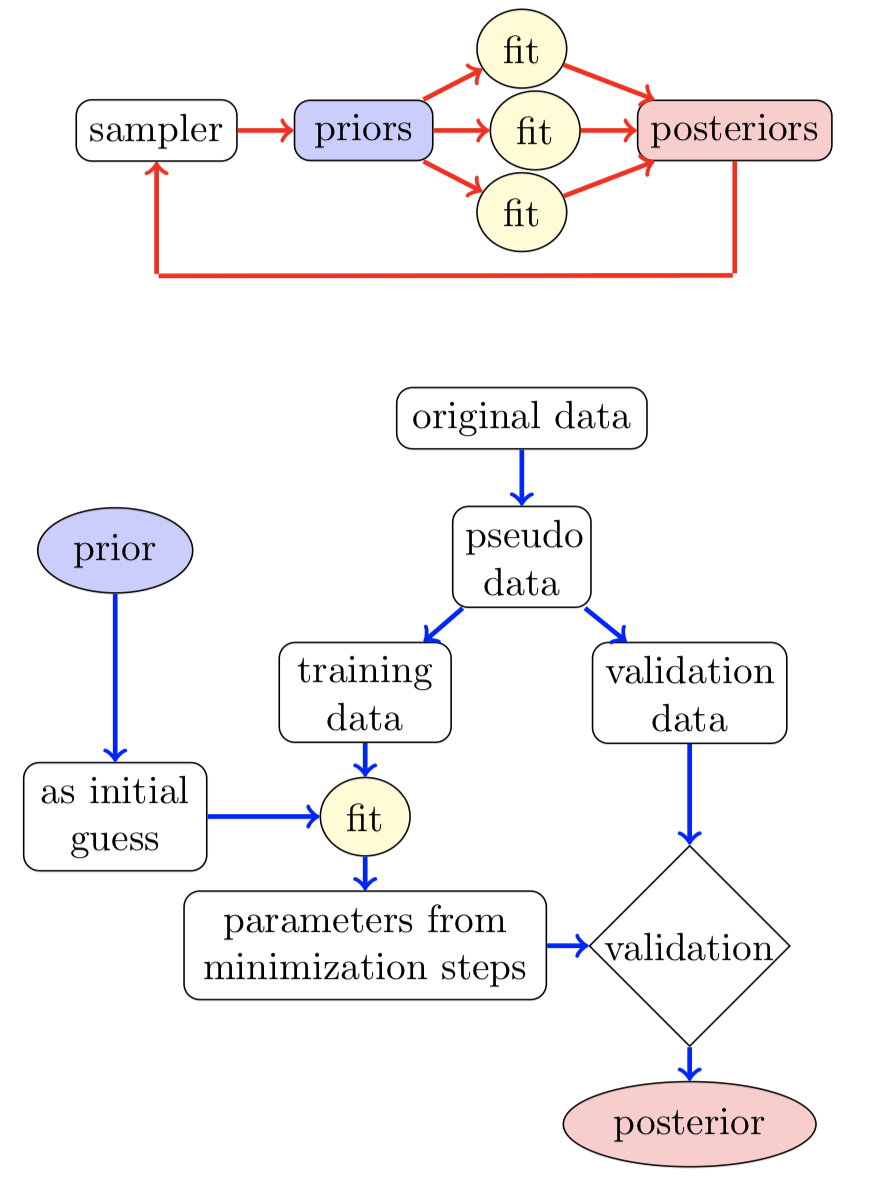
\includegraphics[scale=0.45]{./gfx/IMC.png}
	\caption{Workflow of the iterative Monte Carlo fitting strategy. In the upper diagram (red lines) an iteration begins at the prior sampler and a given number of fits are performed generating an ensemble of posteriors. After the initial iteration, with a flat sampler, the generated posteriors are used to construct a multivariate Gaussian sampler for the next iteration. The lower diagram (with blue lines) summarizes the workflow that transforms a given prior into a final posterior. Figure taken from \cite{IMC}.}
	\label{pic:IMC}
\end{figure}


The functional they use for $D^h_q$ is the following :
%
\begin{equation}
  D^h_i (z,Q_0;\textbf{a}) = M \frac{z^{\alpha}(1-z)^{\beta}}{B(2+\alpha,1+\beta)}
  \label{eq:JAMparam}
\end{equation}
%
where $\textbf{a} = {M,\alpha,\beta,\gamma}$ is the vector of shape parameters to be fitted and $B$ is the Euler beta function. The denominator is chosen so that the coefficient $M$ corresponds to the average momentum fraction $z$. Isospin symmetry is considered for all partons. Using $D^{h^{+}}_{q^{\pm}}(z,Q^2)~=~D^{h^{+}}_{q}(z,Q^2)~\pm~D^{h^{+}}_{\bar{q}}(z,Q^2)$ allows JAM to consider two templates functions for the FFs $D^{\pi^{+}}_{u^{+}}~=~D^{\pi^{+}}_{d^{+}}$, $D^{K^{+}}_{u^{+}}$ and $D^{K^{+}}_{s^{+}}$, which contain both favoured and unfavoured distributions and only one template function for the rest of unfavoured distributions viz. $D^{\pi^{+}}_{\bar{u}}~=~D^{\pi^{+}}_{d}$, $D^{\pi^{+}}_{s}~=~(1/2)D^{\pi^{+}}_{s^{+}}$, $D^{K^{+}}_{\bar{u}}~=~(1/2)D^{K^{+}}_{d^{+}}$ and $D^{K^{+}}_{s}$ along with the heavy quarks and gluons\footnote{The choice of the factor $1/2$ is motivated by data.}.

The favoured and unfavoured FFs from JAM at LO for $Q^2$ = $5$ GeV$^2$ are plotted as a function of $z$ for $\pi^+$ and $K^+$ (Fig.~\ref{pic:JAMcomp}). The strange quark fragmentation into $K^+$ from JAM$17$ is compared with DSS$07$ and HKNS results. While part of the disagreement between fits can be explained by the different parametrizations used, the large uncertainties on the data and the PDFs also play a role.

\begin{figure}[!h]
  \centering
	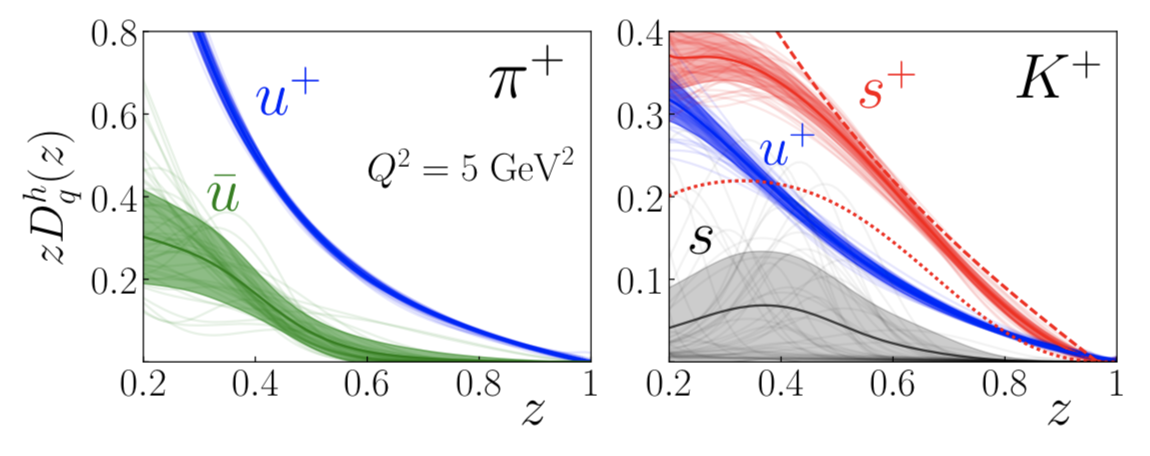
\includegraphics[scale=0.7]{./gfx/JAMcomp.png}
	\caption{Fragmentation functions $zD^h_q$ to $\pi^+$ (left panel) and $K^+$ (right panel) for $u^+$ (blue), $\bar{u}$ (green), $s^+$ (red) and $s$ (grey) at $Q^2$ = $5$ GeV$^2$ for the JAM$17$ analysis, compared to $s^+ \rightarrow K^+$ from DSS$07$ (dashed line) and HKNS (point line). Figure taken from \cite{JAM}.}
	\label{pic:JAMcomp}
\end{figure}

\section{Summary}

The DIS process is a very interesting channel for the study of the nucleon structure. The spin averaged PDFs, mostly determined from inclusive DIS, are well constrained in a wide kinematic domain for the first generation of quarks. Going to higher masses, large uncertainties still subsist e.g. for $s$ and $\bar{s}$. In SIDIS one gets additional access to FFs, which are universal quantities and parametrize quark hadronization.

Several groups have already issued parametrization of quark FFs based on LO and NLO analyses of various data sets. They differ significantly in the strange quark sector. This is why COMPASS did a new measurement and why the analysis presented in this was done.
 % Theoretical framework
% Chapter 2

\chapter{Renormalization and QED Radiative Corrections} % Chapter title

\label{ch:Renorm} % For referencing the chapter elsewhere, use \autoref{ch:name}

%----------------------------------------------------------------------------------------

\section{Divergences, regularization and renormalization in QED}

When calculating loop Feynman diagrams in QED at some point the integrals will diverge. To cure these divergences we have to go through the process of renormalization. Renormalization is a formal manipulation, embedded inside the quantum field theory formalism, which allows us to calculate finite testable expectation values and scattering amplitudes. However we do not know how physics decribes high energy processes : there may be high energy virtual particles contributing to the loop diagrams and they would definitely impact the divergence of the integral. Thus we could say that renormalization is a procedure allowing to calculate reasonably the effects of the low-energy physics independently to what happens at high energies.

To describe the renormalization process, consider the electron self-energy. Defining the full electron propagator $G_F(p)$ by including order-by-order in the perturbation theory the corrections to the Feynman-Green function \cite{ItzyksonZuber} :
%
\begin{equation}
    \begin{split}
      G_F(p) =
      \feynmandiagram [layered layout, horizontal=d to b] {
  b -- [anti fermion] d, };
  +
  \feynmandiagram [layered layout, horizontal=a to b]{
  a -- [anti fermion] b
  -- [anti fermion] c
  -- [anti fermion] d,
  b -- [photon, half left, looseness=1.5] c,};
  +
  \mathscr{O}(e^4_0) \\
      = \frac{i}{\slashed{p}-m_0+i\epsilon} + G^{(1)}_F(p) + \mathscr{O}(e^4_0)
    \end{split}
\end{equation}
%
where $e_0$ and $m_0$ are the \textit{bare} charge and mass parameters and $G^{(1)}_F(p)$ is a divergent term. The renormalization procedure then follows three steps :

\begin{enumerate}
  \item \textbf{Regularization} : set a new \textit{finite} integral $G^{(1)}_F(p,\Lambda)$ with a dependence with the \textit{cut-off scale}\footnote{A cut-off is often introduced in text books to explain the procedure. However, all modern practical calculations are performed with \textit{dimensional regularization}.} $\Lambda$ yielding :
  \begin{equation}
    G^{(1)}_F(p,\Lambda) \xrightarrow{\Lambda\rightarrow\infty} G^{(1)}_F(p)
  \end{equation}
  This integral has a divergent and finite part :
  \begin{equation}
    G^{(1)}_F(p,\Lambda) = I_{div}(p,\Lambda) + I_{fin}(p,\Lambda)
  \end{equation}
  The finite part $I_{fin}(p,\Lambda)$ leads to physically measurable effects and are the \textit{radiative corrections}.

  \item \textbf{Renormalization} : if the theory is \textit{renormalizable} the divergent part can be combined with the tree-level propagator :
  \begin{equation}
    \begin{split}
    G^{(1)}_F(p,\Lambda) = \frac{i}{\slashed{p}-m_0+i\epsilon} + I_{div}(p,\Lambda) + I_{fin}(p,\Lambda) + \mathscr{O}(e^4_0) \\
    = \frac{iZ_2(\Lambda)}{\slashed{p}-m(\Lambda)+i\epsilon} + I_{fin}(p,\Lambda) + \mathscr{O}(e^4_0)
    \end{split}
  \end{equation}
  Thanks to the \textit{wavefunction renormalization} $Z_2(\Lambda)$ and a renormalized mass parameter $m(\Lambda)$, the divergent terms can be integrated into the tree-level propagator.

  \item \textbf{Removing $\Lambda$-dependence} : By taking $\Lambda\rightarrow\infty$, the bare parameters $e_0$ and $m_0$ become singular allowing the physical $e$ and $m$ to be finite. The perturbation expansion is a series in $e$ and not in $e_0$.
\end{enumerate}

This procedure is well-based and defined and give consistent and definite physical results whatever regularization you choose. By definition, a theory is said to be \textit{renormalizable} if all divergences can be removed by renormalization of a finite number of parameters in the Lagrangian.

%----------------------------------------------------------------------------------------

\section{QED Radiative Corrections}

Radiative corrections had a key role in the development of QED : they enable one to calculate cross-sections with extremely high precision that has until now not been contradicted by experiment. When a process like DIS involves charged particles, there is a rearrangement of the electromagnetic current between the initial and final state. Incidentally, real photons can be emitted.

If one were to compute the cross section of the process $1+2 \rightarrow 3+4$ with no photon emission (Born level process), one would find a different result $\sigma_{0}$ than the measurement $\sigma_{exp}$. To obtain a more accurate result, one has to consider the processes $1+2 \rightarrow 3+4+\gamma_1+\gamma_2+..+\gamma_n$. Taking these corrections to Born level process into account, one obtains :
%
\begin{equation} \label{eq:RC}
  \sigma_{exp} = (1+\delta_{RC})\sigma_0,
\end{equation}
%
where $\delta_{RC}$ are the radiative corrections.


In this note, I will not discuss the corrections beyond first order. These first order corrections are also known as order $\alpha$
($o(\alpha)$) corrections. They comprise :
\begin{itemize}
\item Leptonic radiation
\item Hadronic radiation
\item Interference of lepton/hadron radiation (two-photon exchange)
\item Vacuum polarization
\item Weak corrections
\end{itemize}

The goal is to quantify the effect of radiative corrections. The observed cross-section can be expressed as the convolution of the true cross-section times a function called the radiator function which takes into account the radiative effects :
%
\begin{equation}
  d\sigma^{obs}(p,q) = \int \frac{d^{3}k}{2k^{0}}R(l,l',k)d\sigma^{true}(p,-q,k).
\end{equation}
%
A similar relation holds also for the structure functions :
%
\begin{equation}
  F_{n}^{obs}(x,Q^{2}) = \int d\tilde{x}d\tilde{Q}^{2}R_{n}(x,Q^{2},\tilde{x},\tilde{Q}^{2})F_{n}^{true}(\tilde{x},\tilde{Q}^{2}).
\end{equation}
%
The previous formulas are valid for one photon emission but can be extended to include higher-order multi-photon emissions. As one has access to both observed quantities and radiator function, the determination of the true cross-sections or structure functions from measured ones is done by unfolding using an iterative procedure. The principal drawbacks of such a method is that the solution is ill-defined : there is no unique solution, there are large uncertainties and the process is numerically unstable. To stabilize the calculation of the convolution table, i.e. the \textit{folding}, partial fractioning is used on the radiator function :
%
\begin{equation}
  R(l,l',k) = \frac{I}{k.l}+\frac{F}{k.l'}+\frac{C}{\tilde{Q}^{2}}.
\end{equation}
%
The partial fractioning is splitting the radiator function in three :
\begin{itemize}
\item Initial state radiation ($I$ fraction)
\item Final state radiation ($F$ fraction)
\item Compton peak ($C$ fraction)
\end{itemize}

For each of them, an observation can be made. For initial state radiation (ISR), $k.l$ is small for
$\angle (l_{in},\gamma) \rightarrow 0$, for final state radiation (FSR), $k.l'$ is small for
$\angle (l_{out},\gamma) \rightarrow 0$ and eventually for Compton peak $Q^{2}$ is small for
$p_{T}(l_{out}) \simeq p_{T}(\gamma)$.

For ISR and FSR, the photon is emitted within narrow cones with width of the order of $\sqrt{\frac{m_{t}}{E_{t}}}$. The radiated photon can be collinear, but it is not always collinear.
The photon can be collinear independent of whether the radiating particle has a finite mass or is massless. Collinear radiation leads to a divergence if the radiating particle is massless.

Two last notes are to be made :
\begin{itemize}
\item As $E^{2}_{\gamma,max} \propto Q^{2}\frac{1-x}{x}$, the largest radiation in energy are at large $Q^{2}$ and small $x$. Radiation is suppressed at small $Q^{2}$ and large $x$. There are also large negative corrections from uncancelled virtual contributions.
\item As $\tilde{Q}^{2}_{min} = \frac{x^{2}}{1-x}M^{2}_{N}$, the case where $\tilde{Q}^{2}_{min} \ll Q^{2}$ is possible.
\end{itemize}

All the preceding explanations did concern leptonic radiation. One should also address the question of the hadronic corrections (quark line radiation). These corrections are infrared divergent (radiation of soft photons and gluons) but they cancel with loops. The emission of the photon/gluon can be collinear and gives rise to correction of type $\frac{\alpha}{2\pi}log(m_{q}^{2})$. For quarks, the approximation $m_{q} \approx 0$ is giving rise to divergent corrections. One way to solve this issue is to factorize and absorb the divergences into the PDFs :
%
\begin{equation}
  d\sigma = \sum_{f}d\hat{\sigma}_{f}(1+\delta_{f}(Q^{2},m^{2}_{q}))q_{f}(x) = \sum_{f}d\hat{\sigma}_{f}\hat{q}_{f}(x,Q^{2}).
\end{equation}

\subsection{Characterization and impact of radiative corrections in analysis}

In the following, only DIS/SIDIS is considered.

The description of a radiative event is given by the following : an event is called radiative as soon as it contains one real radiated photon which is emitted in the lepton line (Fig. \ref{fig:rad_evt}).

\begin{figure}[htb]
\centering
\begin{tikzpicture} \begin{feynman}
\vertex (i1) {\(l\)};
\vertex[right=1cm of i1] (i3);
\vertex[above right=1cm of i3] (i4) {\(\gamma\)};
\vertex[right=1cm of i3] (a);
\vertex[above right=2cm of a] (i2) {\(l'\)};
\vertex[blob,below=2cm of a] (b) {};
\vertex[below left=2cm of b] (f12) {\(N\)};
\vertex[below=0.1cm of f12] (f13);
\vertex[above=0.1cm of f12] (f11);
\vertex[right=2cm of b] (f22);
\vertex[below=0.3cm of f22] (f23);
\vertex[above=0.3cm of f22] (f21);

\diagram* { (i1) -- [fermion] (i3) -- [fermion] (a) -- [fermion] (i2),
(i3) -- [photon] (i4),
(a) -- [photon, edge label=\(\gamma^*\)] (b) [blob],
(f12) -- [double distance=7pt] (b) [blob] -- [plain] (f22),
(f12) -- [fermion] (b) [blob],
(b) [blob] -- [plain] (f21),
(b) [blob] -- [plain] (f23),
};
\draw [decoration={brace}, decorate] (f21.north east) -- (f23.south east) node [pos=0.5, right] {\(X\)};
\end{feynman} \end{tikzpicture}
\caption{Typical Feynman diagram of a radiative event. One can note that the pair $(Q^2,\nu)$ at the vertex (called hadronic) is not the same as the one calculated using the incoming and outgoing lepton (called leptonic). The relation between the two pairs is drawn by : $\nu_{had} = \nu_{lep} - E_\gamma, Q^2_{had}=Q^2_{lep}+2E_\gamma(\nu_{lep} \sqrt{\nu_{lep}^2+Q^2_{lep}}cos\theta_\gamma)$}
\label{fig:rad_evt}
\end{figure}


In the following, we will only consider these corrections (Fig. \ref{fig:rad_dia}) :
\begin{itemize}
\item Internal Bremsstrahlung (from both incoming and outgoing leptons) (b,c)
\item Vertex correction (d)
\item Vacuum polarization (e)
\end{itemize}

\begin{figure}[htb]
\centerline{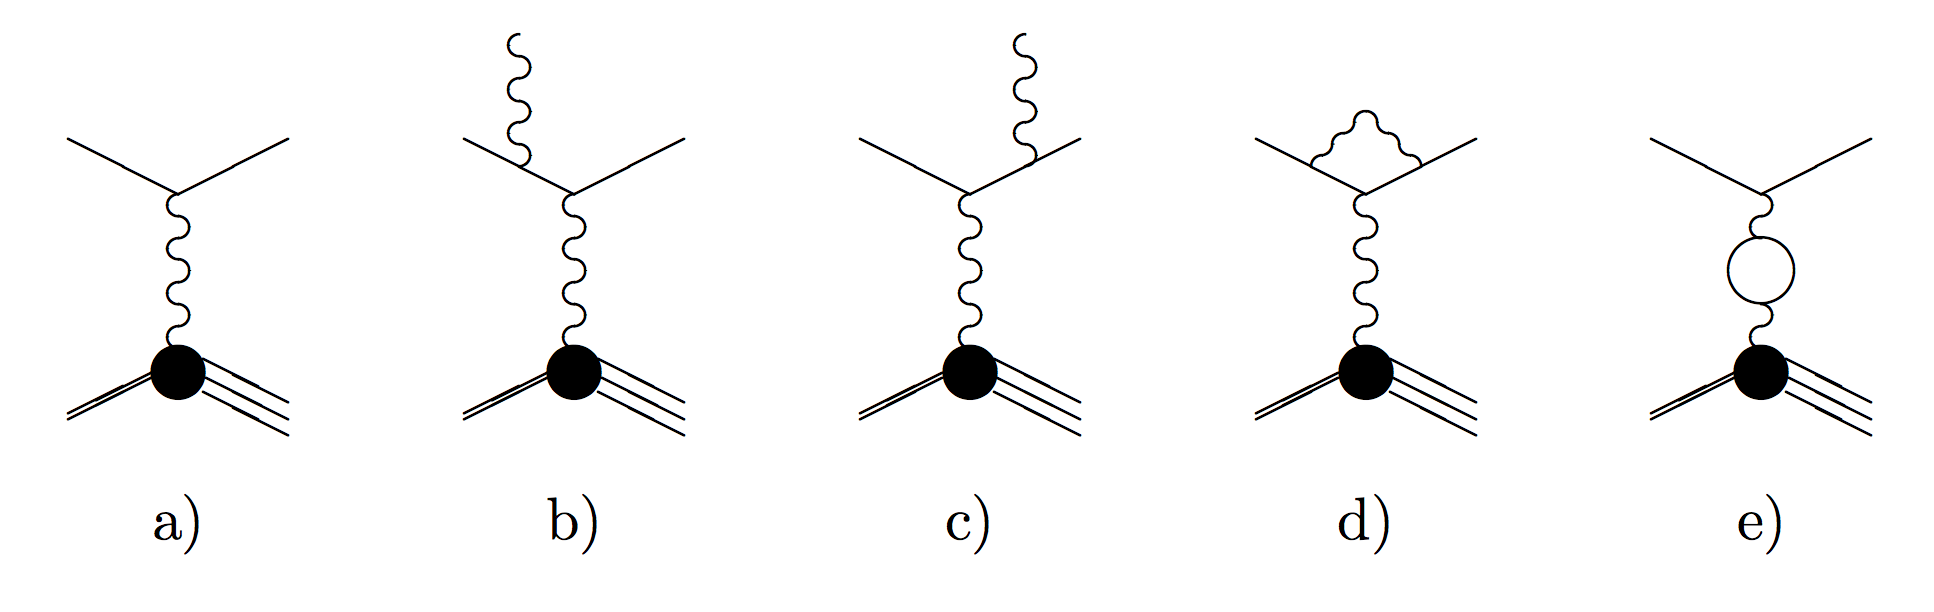
\epsfig{file=gfx/all_rad_feynm.png,width=12cm}}
\caption{List of the diagrams used for the calculation of the radiative corrections. From left to right, tree level, internal bremsstrahlung (incoming and outgoing leptons), vertex correction and vacuum polarization.}\label{fig:rad_dia}
\end{figure}

Correction to the quark line are not included in calculations, as explained in Section \ref{sec:RCF}. If we call $\sigma_{Born}$ the cross-section of the tree-level diagram and $\sigma_{Born+o(\alpha)}$ the cross-section of tree-level plus the first order correction enumerated above, the definition of the radiative corrections factor $\eta$ is :

\begin{equation} \label{eq:RCF_def}
  \eta(x,y)=\frac{\sigma_{Born}(x,y)}{\sigma_{Born+o(\alpha)}(x,y)}
\end{equation}

Obviously, the emission of a real photon is modifying the kinematic variables of the event. Let us take the case of one DIS event and a second one which is exactly like the first one except there is an ISR. The two events will share the same leptonic variables but they will have different hadronic variables. In the case of multiplicities, this discrepancy in the kinematic variables induces that some hadrons are falling into the wrong (x,y) bin. Applying the correction factor $\eta$ to the multiplicities is redirecting the hadrons to the right (x,y) bins.

\subsection{About emission of radiative photons}

There are two privileged angles (Fig. \ref{fig:plan}) for emission of a real photon :
\begin{itemize}
\item One in the direction of the incident lepton (s-peak)
\item One in the direction of the outgoing lepton (p-peak)
\end{itemize}

\begin{figure}[h!]
\centering
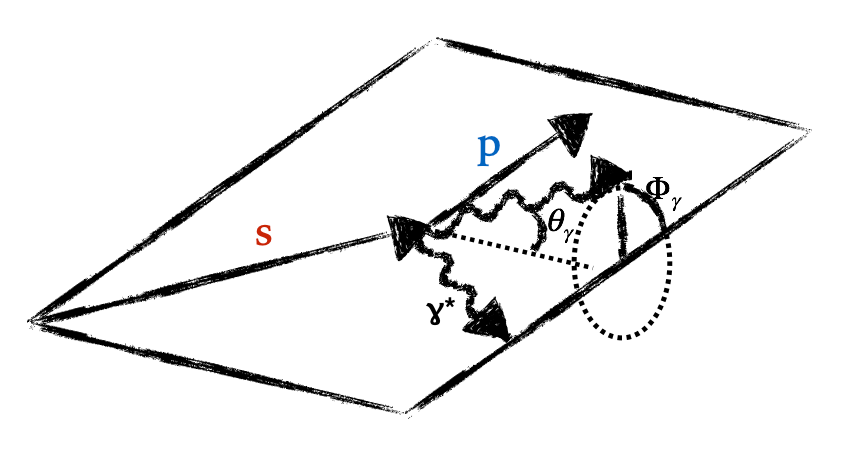
\includegraphics[width=12cm]{gfx/plan_angle.png}
\caption{Angles characterizing the emission of a radiative photon. The plane is defined by the incoming lepton (s) and the outgoing lepton (p). $\theta_\gamma$ is the polar angle and $\Phi_\gamma$ the azimuthal angle. Figure taken from \cite{TERAD2}.}
\label{fig:plan}
\end{figure}

In the case of muons, note that the $s$ and $p$ peaks are much less pronounced than for electrons.

This knowledge will later be useful to verify the consistency of DJANGOH results.

\subsection{About the radiative tail}

During elastic events, radiation of a real photon can still happen, modifying the leptonic variables of the events : this is the radiative tail. With Fig. \ref{fig:peaks}, we can see that even if we measure DIS events i.e. $Q^2$ $>$ 1, we still need informations on structure functions down to $Q^2$ = 0.

\begin{figure}[h!]
\centering
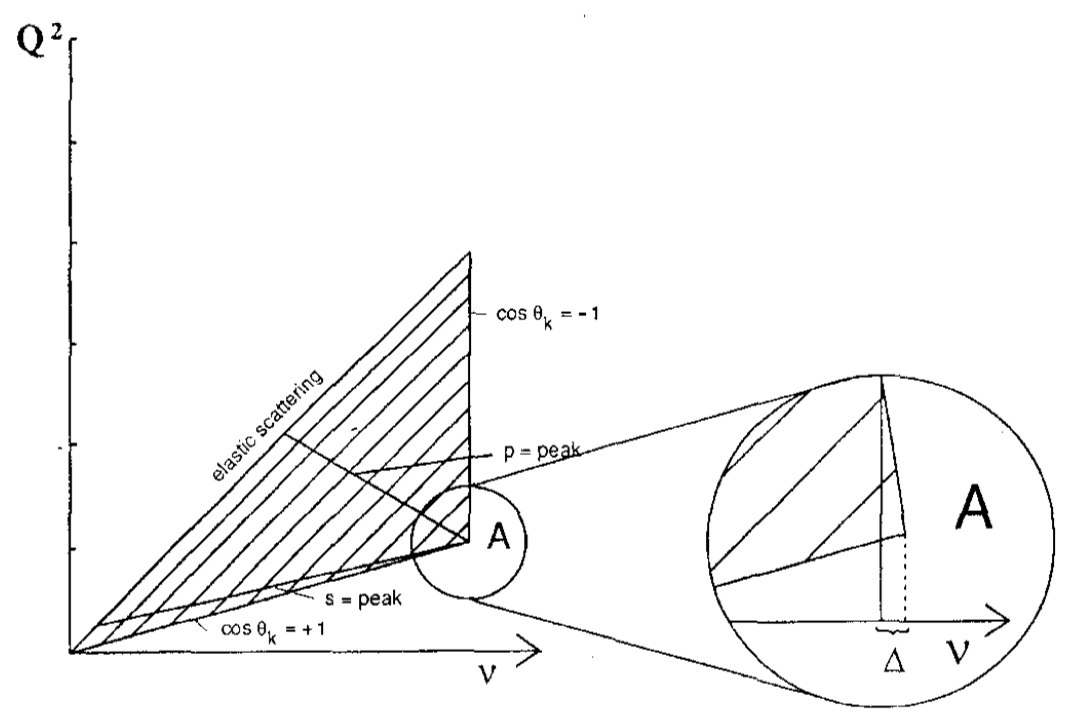
\includegraphics[width=12cm]{gfx/peaks.png}
\caption{Range of kinematical variables from which the radiative tails contribute to the cross section
measured at the point $A(Q^2, \nu)$. The s-peak is located near the boundary $cos\theta_\gamma=1$ which means
$\theta_\gamma \equiv 0[2\pi]$, thus collinear to the incoming lepton. The parallel lines are for constant $W$. Figure taken from \cite{TERAD2}.}
\label{fig:peaks}
\end{figure}

\newpage

%----------------------------------------------------------------------------------------

\section{Summary}

The renormalization is a necessary procedure when it comes to compute cross-sections as it allows to cure the divergences from the calculation and gives consistant results when compared to measurements. From this renormalization procedure arise radiative corrections which imply the emission of a real photon in the final state. These corrections can be splitted in three groups : from the Initial State Radiation (ISR), from the Final State Radiation (FSR) and from the Compton Peak. The emission of a real photon implies that there is a difference between the hadronic and leptonic variables that must be taken into account. Radiative correction factor are computed to measure the effect of the kinematic bin migration and correct the data accordingly.
 % Renormalization and QED Radiative Corrections

\cleardoublepage % Empty page before the start of the next part

%------------------------------------------------

\part{Experimental Part} % Second part of the thesis

% Chapter 3

\chapter{The COMPASS experiment at CERN} % Chapter title

\label{ch:exp} % For referencing the chapter elsewhere, use \autoref{ch:name}

In this chapter a description of the COMPASS experiment is provided. The general features of the spectrometer are given in Section~\ref{sec:specgen}. The beam and target are presented in Section~\ref{sec:beam}. The descriptions of the detectors used for the tracking and the ones used for the particle identification are respectively done in Section~\ref{sec:track}. The trigger system is discussed in Section~\ref{sec:trigger}. Eventually the last sections deal with data acquisition and reconstruction.

%----------------------------------------------------------------------------------------

\section{General Overview}\label{sec:specgen}

COMPASS is a high energy, high rate fixed-target experiment at the Super Proton Synchrotron (SPS) at CERN. It is dedicated to the study of hadron structure and hadron spectroscopy with high intensity muon and hadron beams.

In order to cover the necessary large range in $Q^2$ and $x$ for the available beam energy the COMPASS spectrometer as shown in Fig.~\ref{pic:apparatus} covers a large in particle momentum and angle. Such range is obtained with a wide trigger coverage.

The apparatus is divided in three parts : the first part is dedicated to the detection of the incoming beam and is located upstream the target location. The second and third part are located downstream of the target and represent a length of $50$ meters. The second part called the \textit{Large Angle Spectrometer} (LAS) is built around the magnet SM$1$.
The LAS has been designed to provide a $180$ mrad acceptance. The \textit{Small Angle Spectrometer} (SAS), built around the magnet SM$2$, measures the particles emitted at small angles ($\pm$ $30$ mrad).

In $2016$, the data taking was performed with a $160$ Gev/c muon beam scattering off a liquid H$_2$ target.

\begin{sidewaysfigure}[!p]
  \centering
	\subfloat[LAS]{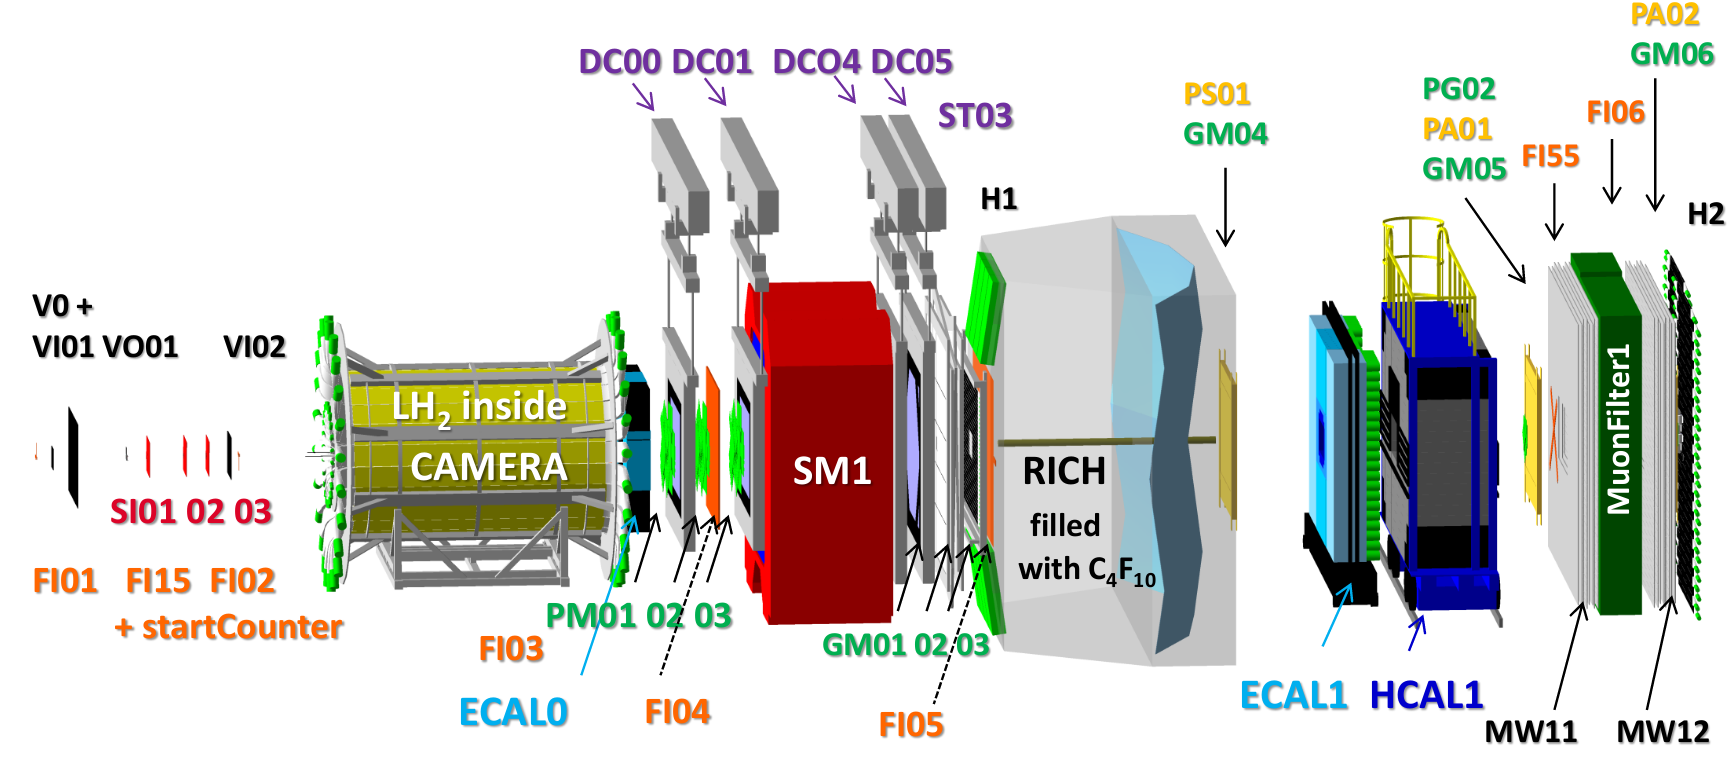
\includegraphics[scale=0.28]{./gfx/Apparatus1.png}}
  \subfloat[SAS]{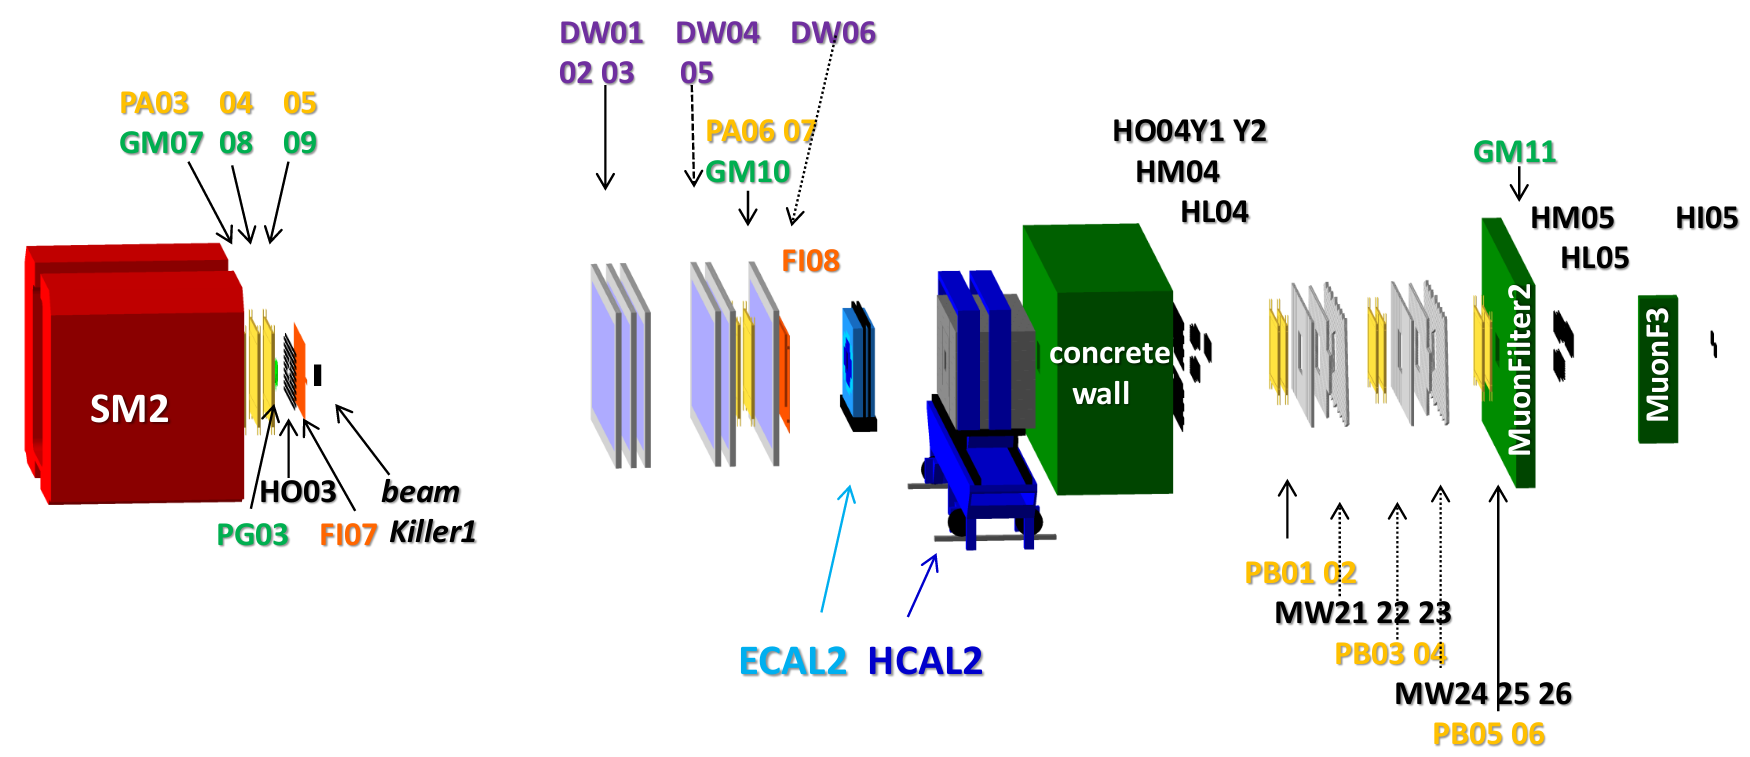
\includegraphics[scale=0.28]{./gfx/Apparatus2.png}}
	\caption{COMPASS 2016/2017 muon setup side view. Taken from \cite{Setup}.}
	\label{pic:apparatus}
\end{sidewaysfigure}

%----------------------------------------------------------------------------------------

\section{Beam}\label{sec:beam}

The muon beam used by COMPASS is obtained from a primary proton beam accelerated in the SPS up to $400$ GeV/c. The proton beam interacts with T6 target, a $50$ cm thick beryllium target, producing mainly pions and kaons. The spill time, which is the time period window within which the proton beam is delivered to the T6 target, is of $4.8$ s. In each cycle of $36$ s there are two spills.

\subsection{The M$2$ Beam Line}

The produced hadrons are transported in a $600$ m long channel of the M$2$ beamline \cite{NIM2015,M2Beam}. During this time, $5$\% of the pions and kaons are decaying into muons and neutrinos. At the end of this $600$ m decay section, remaining hadrons are stopped by a hadron absorber and the muons are focused. A system of magnets is then used to select and focus the muons of $160$ GeV/c.

The beam has transverse dimensions of $\sigma_x \times \sigma_y \sim 8 \times 8 $ mm$^2$ and an angular divergence of $\sigma_{\theta_x} \times \sigma_{\theta_y} \sim 0.5 \times 1 $ mrad$^2$ in the experimental area. At each spill, $2.10^8$ muons enter the experimental area. The beam is accompanied by a muon halo that extends transversely up to several meters of distance with respect to the beam line. The intensity of this halo decreases with the distance. The halo near the beam line as measured by a $30 \times 30$ cm$^2$ dedicated veto counter with a 4 cm diameter central hole represents $\sim$ 16\% of the muon beam. The far halo or low intensity halo is measured by a large veto counter with a central hole of $30 \times 30$ cm$^2$. It represents $\sim$ 7\% of the muon beam.

\subsection{The Beam Momentum Station}

The Beam Momentum Station (BMS) illustrated in Fig.~\ref{pic:BMS} is used for the determination of the incident muon momentum. It consists of six scintillators hodoscopes (BM$01$-BM$06$) located asymmetrically upstream and downstream a bending magnet (B$6$ : three consecutive dipole magnets) surrounded by four quadrupoles (Q$29$-Q$32$).

The BMS system was designed to measure the momentum of more than $10^8$ individual particles per spill with a relative precision of $0.5$\%. To eliminate the ambiguities in the reconstruction of particle trajectories, their time of transit is measured with a resolution of $50$~ps.

\begin{figure}[!h]
  \centering
	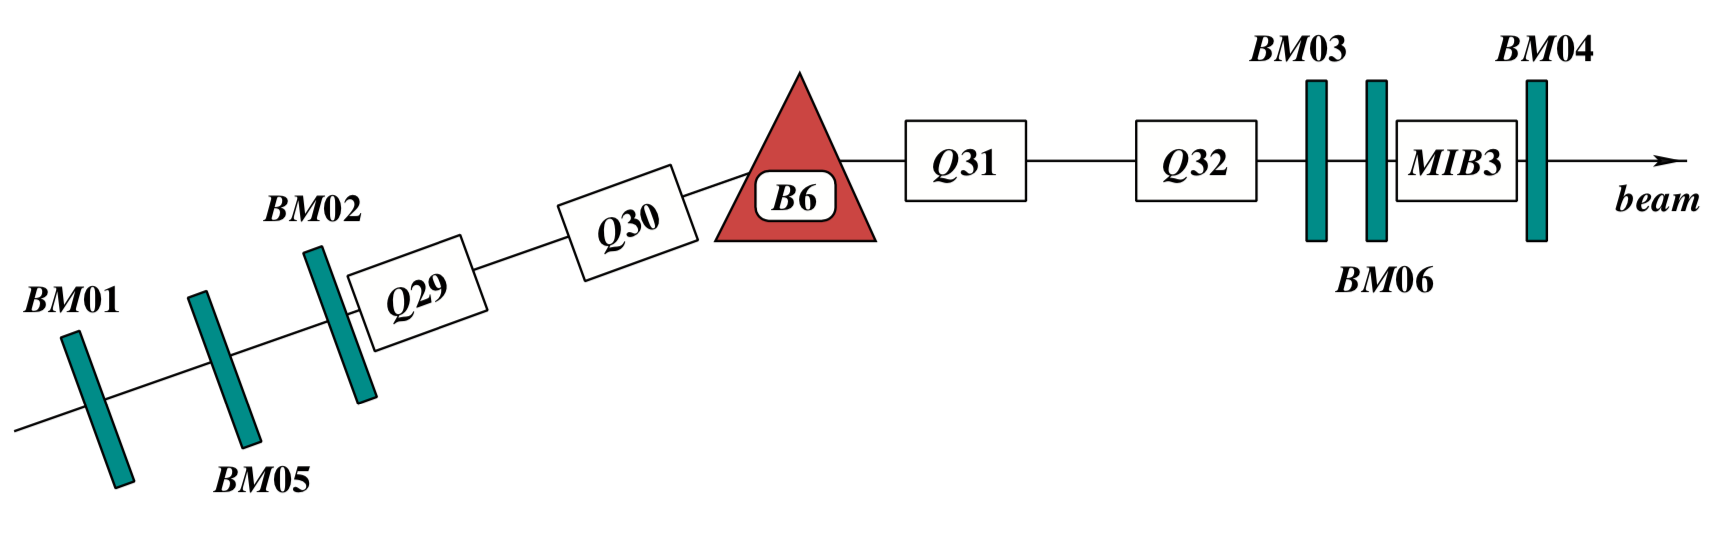
\includegraphics[scale=0.5]{./gfx/BMS.png}
	\caption{Layout of the Beam Momentum Station for the COMPASS muon beam. Taken from \cite{NIM}.}
	\label{pic:BMS}
\end{figure}

%----------------------------------------------------------------------------------------

\section{Target}

\begin{figure}[!h]
  \centering
	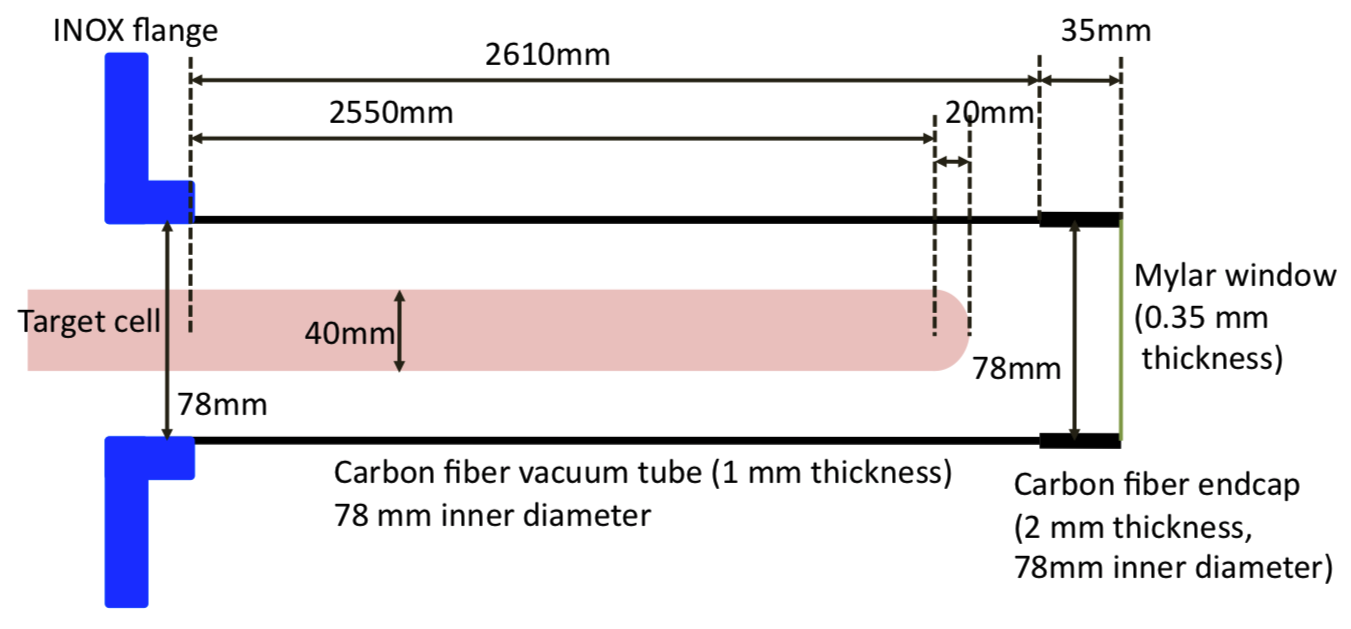
\includegraphics[scale=0.3]{./gfx/Target.png}
	\caption{Target geometry for the 2016/2017 setup.}
	\label{pic:Target}
\end{figure}

The target is liquid $H_2$ contained in a $2.5$ meter long cylinder with a radius of $2$ cm and contains lH$_2$ (Fig. \ref{pic:Target}). The target material is contained in a mylar tube with a diameter of $4$ cm. The total volume of the target cell and the liquid hydrogen system is located in a cryostat made of carbon fiber. The operation temperature of hydrogen is $18$ K with a pressure of $1020$ mbar. The material for the target cell were chosen in order to maximise acceptance.

%----------------------------------------------------------------------------------------

\section{Tracking Detectors}\label{sec:track}

The \textit{Large Angle Spectrometer} (LAS) and \textit{Small Angle Spectrometer} (SAS) are each equipped with different type of tracking detectors. Depending on the direction coverage area of each detectors they are classified as :
\textit{very small area trackers}, \textit{small area trackers} and \textit{large area trakers}

\subsection{Very small area trackers}

The very small area trackers cover the transverse beam size up to $\sim$ $3$ cm. In this region the particle rate is very high ($10^5$/s/mm$^2$ in the center of the muon beam), hence the tracking detectors must have an excellent time and position resolutions.

The scintillating fibre detectors are used at several locations of the experiment and cover areas between $\sim$ $16$ cm$^2$ and $144$ cm$^2$. They are fabricated from $0.5$-$1$ mm diameter fibres and reach a time resolution better than $500$ ps. All along the apparatus there are $9$ stations composed by two or three scintillating fiber detectors. The third detector is always pivoted by $45$° with respect to the others.

The silicon detector size is $5$x$7$ cm$^2$ with a space and time resolution of $\sim$ $10$ $\mu$m and $<$~$2.5$~ns. The $3$ silicon detectors stations are located upstream the target. The stations are each composed by two silicon detectors, the second one being rotated by $5$° with respect to the other, each detector measuring perpendicular views.

\subsection{Small area trackers}

The radial region between $2.5$ cm and $20$ cm is covered by two types of gaseous detectors : Micromegas (MICRO MEsh GAseous Structure) and GEM (Gas Electron Multiplier) detectors. These detector have a high rate capability ($\sim$ $10^4$/s/mm$^2$) and good spatial resolution ($<$ $100$ $\mu$m). They also present a minimal material budget.

The principle of the Micromegas is explained in Fig.~\ref{pic:MM}. The particle ionizes the gas in the conversion gap, the produced electrons drift in a moderate field of $1.5$ kV/cm to prevent secondary ionization, towards the amplification gap. The field in the amplification zone is large enough to accelerate the electrons to produce an avalanche. The conversion and amplification gaps are separated by a \textit{micromesh}, which collects the positive ions produced during the avalanche in a short period of time ($<$ $100$ ns). This feature is possible because of the small width of the gap ($\sim$ $100$ $\mu$m). All Micromegas detectors operate with a detection efficiency of $98$\% and with a spatial resolution of better than $100$ $\mu$m. There are three Micromegas stations located at LAS. They are composed by four detectors each with different directions : horizontal (X), vertical (Y), and two (U,V) rotated by $\pm$ $45$° with respect to the vertical. Each plane has an active area of $40 \times 40$ cm$^2$ with a deactivated central zone of $5$ cm diameter.

\begin{figure}[!h]
  \centering
	\subfloat[]{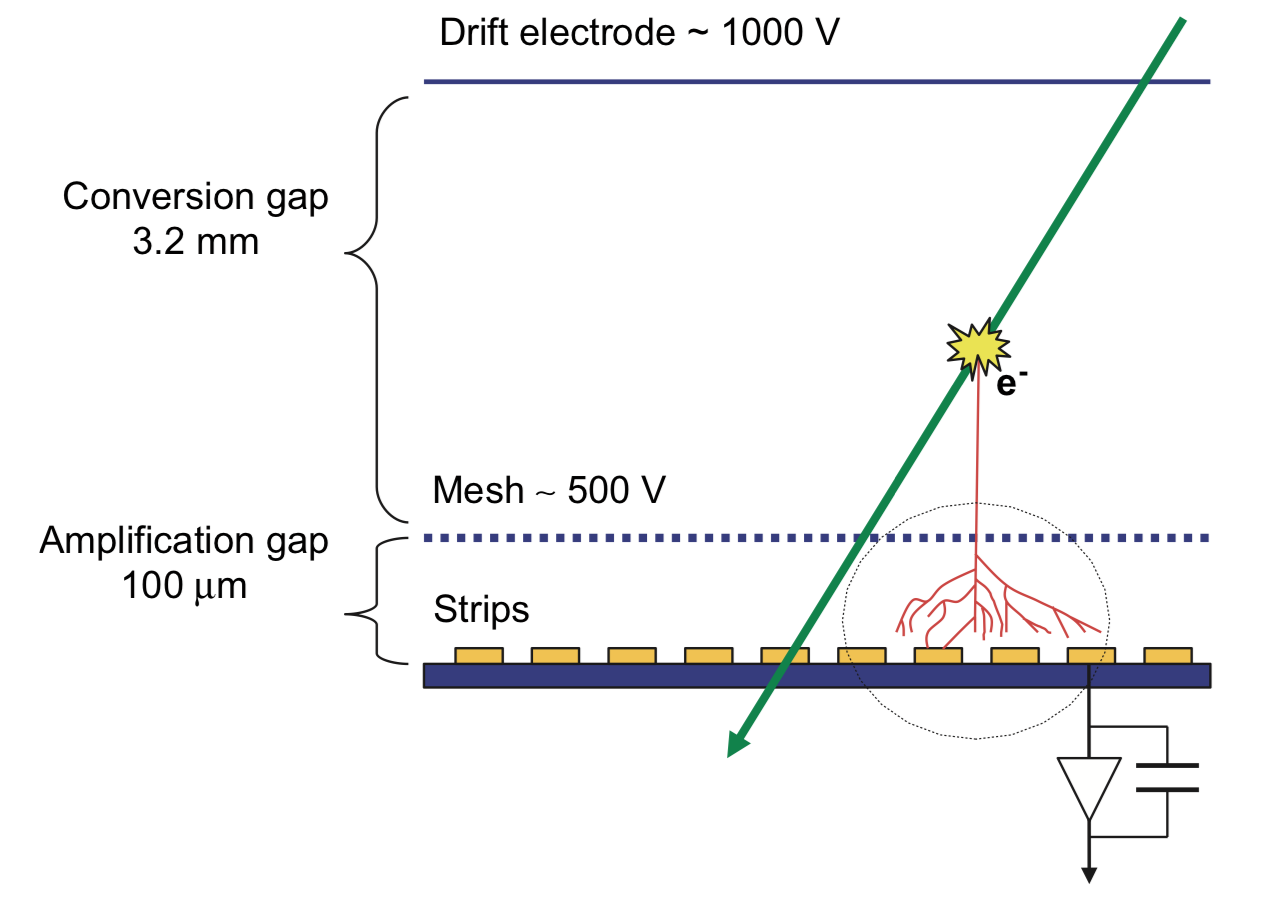
\includegraphics[scale=0.35]{./gfx/MM1.png}}
  \subfloat[]{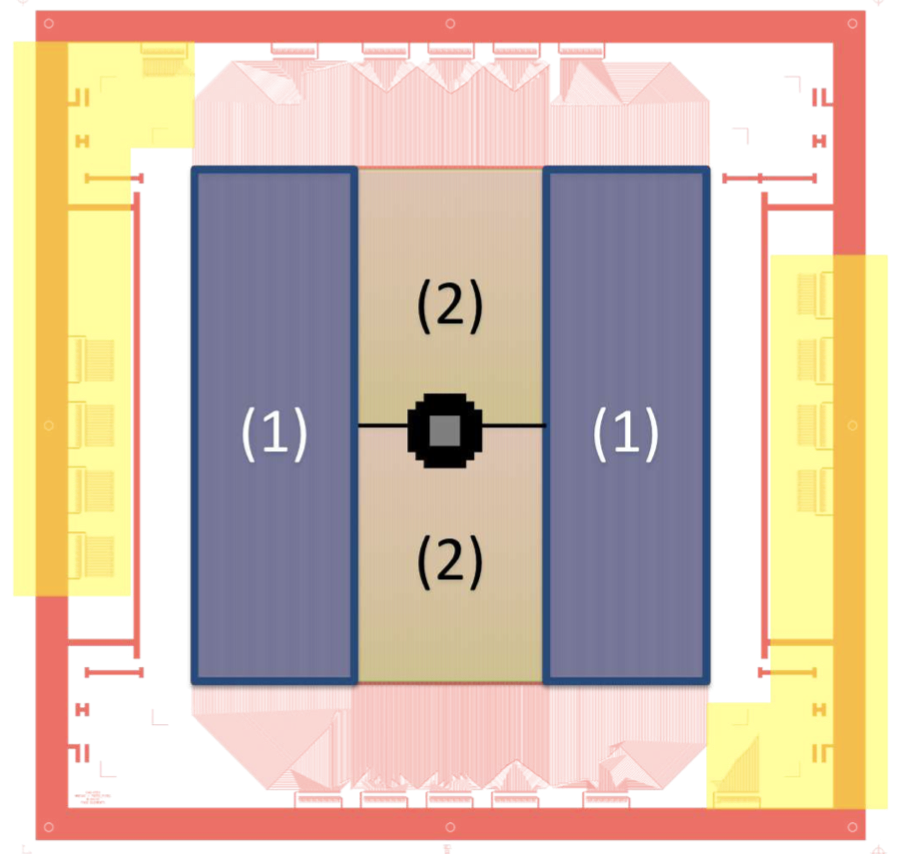
\includegraphics[scale=0.35]{./gfx/MM2.png}}
	\caption{(a) COMPASS MicroMegas detection principle. (b) MicroMegas detector. Taken from \cite{NIM}.}
	\label{pic:MM}
\end{figure}

A GEM is a $50$ $\mu$m thin polyimide foil with Cu cladding on both sides, into which numerous microholes ($\sim$ $10^4$/cm$^2$) with a diameter of $70$ $\mu$m have been chemically etched using lithographic techniques. This allows to limit gain per stage and still have high efficiencies. A high voltage (several $100$ V) is applied to each foil to generate the avalanche multiplication of the electron through the holes. The fast signal is induced by the electron cloud emerging from the last GEM foil on an anode segmented into two sets of $768$ orthogonal strips (pitch of $400$ $\mu$m). The COMPASS GEM detection principle is shown in Fig.~\ref{pic:GEM} : it consists of three GEM amplification stages separated by thin grids of $2$ mm height. A GEM station is composed by $2$ detectors oriented by $45$° relatively to each other. All in all there are $11$ stations, all located at SAS. The active area for the GEM is $31 \times 31$ cm$^2$ and the central area of $5$ cm diameter can be activated to align the detector with low intensity beams. The detectors efficiency is $\sim$ $97$\% with a spatial and time resolution of about $\sim$ $70$ $\mu$m and $12$ ns, respectively.

\begin{figure}[!h]
  \centering
	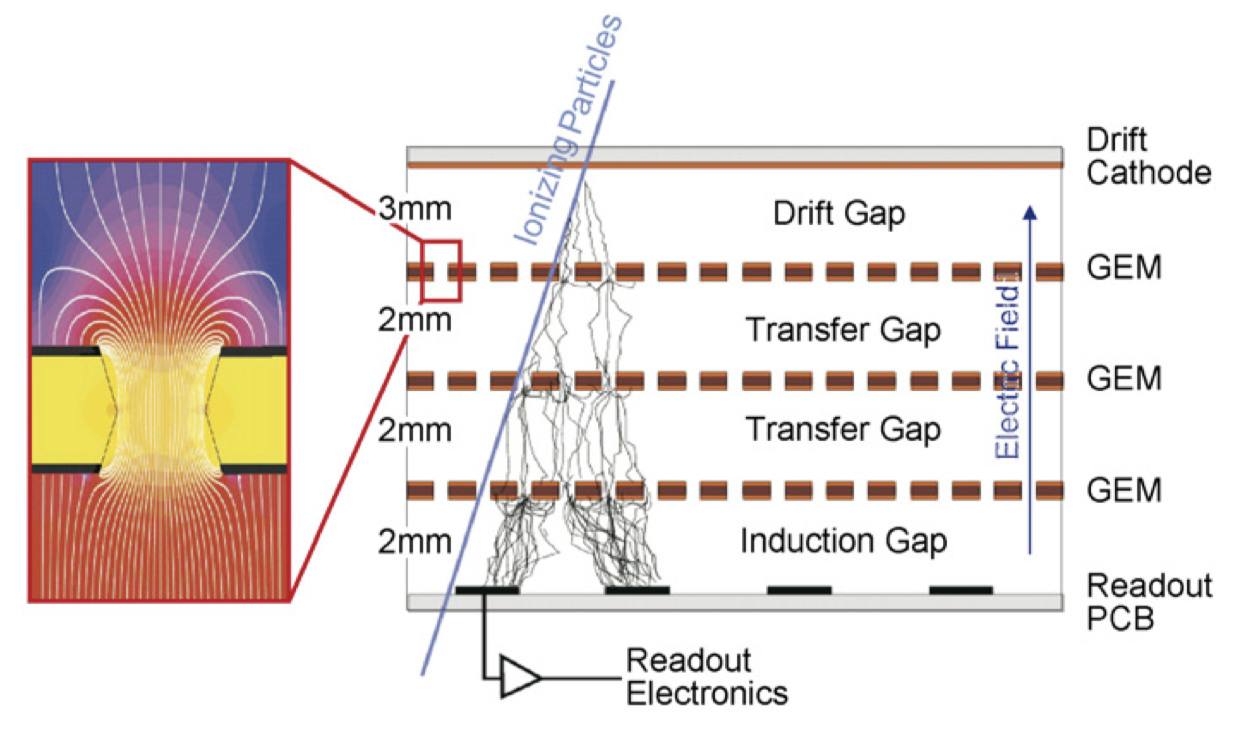
\includegraphics[scale=0.5]{./gfx/GEM.png}
	\caption{COMPASS GEM detection principle. Taken from \cite{NIM}.}
	\label{pic:GEM}
\end{figure}

\subsection{Large area trackers}

The large area trackers cover all the spectrometer acceptance with a good spatial resolution. As the particle rate in the region covered by the large area trackers is small in comparison to the central region ($10^2$/s/mm$^2$), the use of detectors such as drift chambers (DCs and W$4/5$) \cite{DaCosta}, straw drift tubes \cite{Zvyagin} and multiwire proportional chambers (MWPCs) is possible. These detectors have large active size area ($\sim$ m$^2$) with a central dead zone of few cm$^2$.

Each DC consists of eight layers of wires with four different inclinations : horizontal, vertical and rotated $\pm$ $20$° with respect to the vertical direction (X, Y, U and V). Two consecutive planes with the same inclination are staggered by $3.5$ mm to disimbiguate left-right and the ordering of the planes with different orientations is such to minimize the fake track combinations. The detectors are filled with a gas mixture of Ar, C$_2$H$_6$ and CF$_4$ at a volume ratio $9:9:2$. Two of the DC are located before SM$1$ and have an active area of $180 \times 127$ cm$^2$~; the last two are located downstream SM$1$ and have a larger active area of $204 \times 204$ cm $^2$. All these DCs have a central dead zone of $30$ cm. The central dead zone can be activated for alignment needs with a low intensity beam. The average resolution of a DC is $270$ $\mu$m and the efficiency above $95$\%.

The W$4/5$ detectors have an active area of $5$ x $2.5$ m$^2$, and consist of $4$ anode wire layers with a wire pitch of $4$ cm. The anode wires are separated by layers of cathode wires with a pitch of $2$ mm. The diameter of the anode wire is $20$ $\mu$m and of the potential wires, $200$ $\mu$m. A CF$_4$-based gas mixture, Ar/CF$_4$/CO$_2$ ($85/10/5$), is used.

A straw detector station consists in $3$ straw detectors with different orientations : horizontal, vertical and rotation by $10$° with respect to the vertical. The only station used is located between SM$1$ and SM$2$. Each detector is composed by two layers of straw tubes with the same orientation. The straw tubes consist in two layers of thin plastic film, one coated with carbon loaded Kapton, the other one with aluminised Kapton foil. The active area for the straw detector is $320 \times 280$ cm$^2$ and have a central dead zone of $20 \times 20$ cm. The average resolution is of $190$ $\mu$m.

There are three types of MWPCs in COMPASS, which differ by the number of layers, the size of the dead zone for the beam and the combination of the measured projections (X, Y, U and V). The active area is of $178 \times (90-180)$ cm$^2$. All layers have a wire length of about $1$ m, a wire diameter of $20$ $\mu$m and a pitch of $2$ mm and are enclosed on both sides by graphite-coated Mylar foils. The central deadzone of each detector increases with respect to the detector position, from $16$ to $22$ cm. The average spatial resolution of the MWPC is of $1.6$ mm.

\begin{table}[!h]
  \caption{Table with the characteristics of a selection of tracking detectors.}
  \label{tab:kinvar}
  \centering
  \begin{tabular}{c|c|c|c}
    \hline
    \hline
    Detector type & Active area & Spacial resolution & Time resolution \\
    \hline
    \hline
    Scintillating Fibre & $(3.9)^2$ - $(12.3)^2$ cm$^2$ & $130$ - $210$ $\mu$m & $400$ ps \\
    Silicon Micro-strip & $5$ x $7$ cm$^2$ & $8$ - $11$ $\mu$m & $2.5$ ns \\
    GEM & $31$ x $31$ cm$^2$ & $70$ $\mu$m & $12$ ns \\
    Micromega & $40$ x $40$ cm$^2$ & $90$ $\mu$m & $9$ ns \\
    MWPC & $178$ - $(90-120)$ cm$^2$ & $1.6$ $\mu$m & N/A \\
    DC & $180$ - $127$ cm$^2$ & $190$ - $500$ $\mu$m & N/A \\
    Straws & $280$ - $323$ cm$^2$ & $190$ $\mu$m & N/A \\
    \hline
    \hline
  \end{tabular}
\end{table}

%----------------------------------------------------------------------------------------

\section{Particle Identification}

Particle identification is performed by all the tracking detectors. A RICH detector allows to separate between pions, kaons and protons at high intensity environment. Two types of calorimeters are used to measure the energy of the hadrons, photons and electrons : hadrons calorimeters (HCAL1 and HCAL2) and electromagnetic calorimeters (ECAL1 and ECAL2). Two muon wall detectors (MW1 and MW2) are performing muon identifications and consist of tracking detectors combined with a hadron absorber. While the RICH will be further described in a dedicated chapter (Chapter~\ref{ch:PID}), the other identification detectors will be briefly described in the following subsections.

\subsection{Hadron Calorimeters}

A hadron calorimeter allows to separate hadron and muon tracks on the energy deposit. Contrary to a hadron, which deposits almost all its energy via a hadron shower, the muon suffers on energy loss by only deposit a small energy fraction. HCAL$1$ and HCAL$2$ are sampling calorimeters with a modular structure with iron and scintillator plates and are located before the muon filters. Their efficiency depends on the energy : for HCAL$1$ for hadrons with momenta above $5$ GeV/$c$ it is almost constant and close to $100$\% when for HCAL$2$ the same efficiency is reached for hadrons with momenta above $10$ GeV/$c$.

\subsection{Electromagnetic Calorimeters}

The electromagnetic calorimeters are used to measure the energy of electrons and photons. ECAL$1$ and ECAL$2$ are formed by blocks of lead glass connected to photomultipliers with light guides. An electromagnetic shower is initiated when the incoming electrons of photon reach the calorimeter. This electromagnetic shower produces Cherenkov radiation inside the lead glass and this light intensity is proportional to the energy deposited. The inner-most part of ECAL$2$ has radiation-hard Shashlyk-type lead/scintillator modules.

\subsection{Muon Identification with Muon Walls and Muon Filters}

An efficient way to identify muons is to use an absorber surrounded by two tracking detec- tors. With a radiation length large enough to absorb all hadrons, particles detected behind the absorber are considered muons. At COMPASS, this is done in the LAS with the Muon Wall $1$ (MW$1$) and the Muon Filter $1$ (MF$1$). In the SAS, the Muon Wall $2$ (MW$2$) in combination with the Muon Filter $2$ (MF$2$) identify the muons. At the very end of the spectrometer, the Muon Filter $3$ (MF$3$) is the last muon filter detector. The three muon filters are made of steel or concrete. The MW$1$ system consists of Mini Drift Tubes. The tubes are made of $0.6$ mm thick aluminum tubes surrounding a $50$ $\mu$m thick tungsten wire. The muon filter surrounded by the MW$1$ system is made of $60$ cm of steel. The active areas are $4845$ x $4050$ mm$^2$ (hole: $1445$ x $880$ mm$^2$) and $4730$ x $4165$ mm$^2$ (hole: $1475$ x $765$ mm$^2$) for the X and Y planes. The gas mixture of MW$1$ is Ar/CO$_2$ ($70/30$). The MW$2$ system in the SAS has two identical stations of layers of drift tubes. Each of the two stations consists of $6$ layers with an active area of $4470$ x $2020$ mm$^2$. A gas mixture of Ar/CH$_4$ ($75/25$) is used. The stainless steel drift tubes have an inner diameter of $29$ mm and a wall thickness of $0.5$ mm and the wires are $50$ $\mu$m thick.

%----------------------------------------------------------------------------------------

\section{The Trigger System}\label{sec:trigger}

The trigger system \cite{TriggerSys} has the task to select physic event candidates in a high rate environment. It is composed by scintillator hodoscope, complemented by scintillator veto detectors to suppress halo muons and by calorimeters to select events with hadron production. In the central region MWPCs complements the coverage of the muon acceptance.

\begin{table}[!h]
  \caption{COMPASS triggers with the muon beam in 2016.}
  \label{tab:kinvar}
  \centering
  \begin{tabularx}{7.5cm}{cc}
    \hline
    \hline
    Trigger name & Components \\
    \hline
    \hline
    Middle Trigger (MT) & HM$04$, HM$05$ \\
    Ladder Trigger (LT) & HL$04$, HL$05$ \\
    Outer Trigger (OT) & HO$03$, HO$04$ \\
    LAS Trigger (LAST) & H$1$, H$2$ \\
    \hline
    \hline
  \end{tabularx}
\end{table}

Depending on the event kinematics two different algorithms are used to determine the scattered muon kinematics. When the angle of the scattering muon is large enough ($Q^2 > 1$ (GeV/$c$)$^2$) to be measured by using only the hodoscope stations, the trigger signals are built using the vertical pointing algorithm (Fig.~\ref{pic:triglogic}).

\begin{figure}[!h]
  \centering
	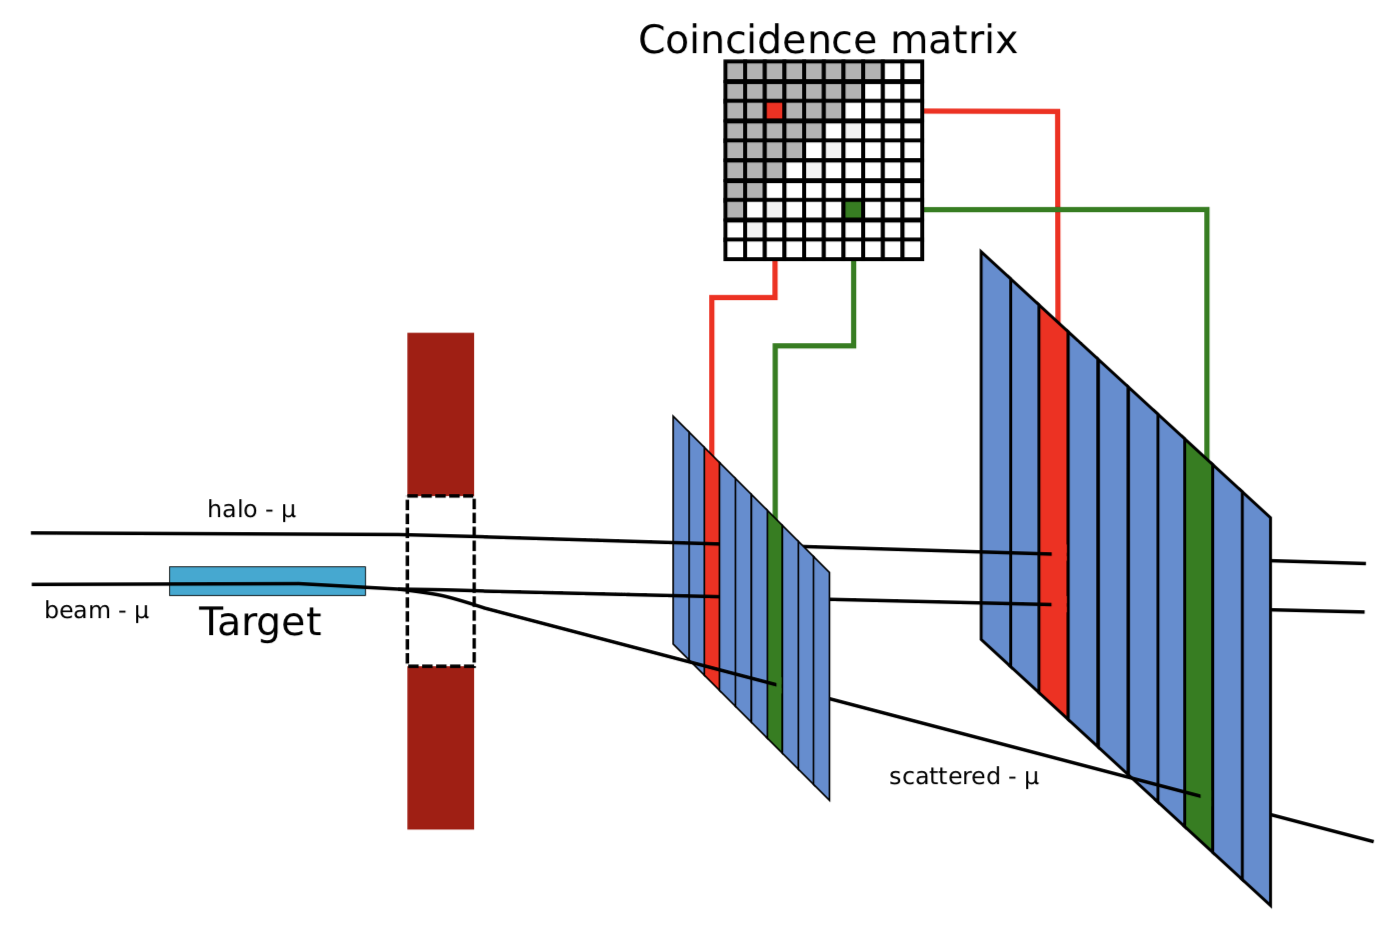
\includegraphics[scale=0.5]{./gfx/TriggerLogic.png}
	\caption{Concept of the trigger. The scattered muon leads to a coincidence in the activated area of the coincidence matrix while the halo muon fails to do so.}
	\label{pic:triglogic}
\end{figure}

The angle ($\theta_x,\theta_y$) of the scattered muon is determined by using two hodoscopes with horizontal strips located at different positions along the beam direction and the vertical component $\theta_y$ is determined. If $\theta_y$ is compatible with the target position the trigger system validates the event. The $y$-$z$ plane is selected since the particle track is not deflected by the dipole magnet in y-direction. In cases where the scattering angle of the muon is too low to be measured ($Q^2 < 1$ (GeV/$c$)$^2$), the bending angle of the magnet is used to determine $\theta_x$ and to perform an energy loss measurement to fire the trigger. This is possible since the muon energy loss $\nu$ is translated into a deflection by the magnetic dipole field.

The kinematic range covered by the trigger system is shown in Fig.~\ref{pic:trigger}. The trigger system is optimized to select DIS events. The lowest $Q^2$ events are covered by the \textit{ladder} trigger (LT) followed by \textit{middle} trigger (MT), \textit{outer} trigger (OT) and \textit{LAS} trigger (LAST) with increasing $Q^2$.

\begin{figure}[!h]
  \centering
	\subfloat[]{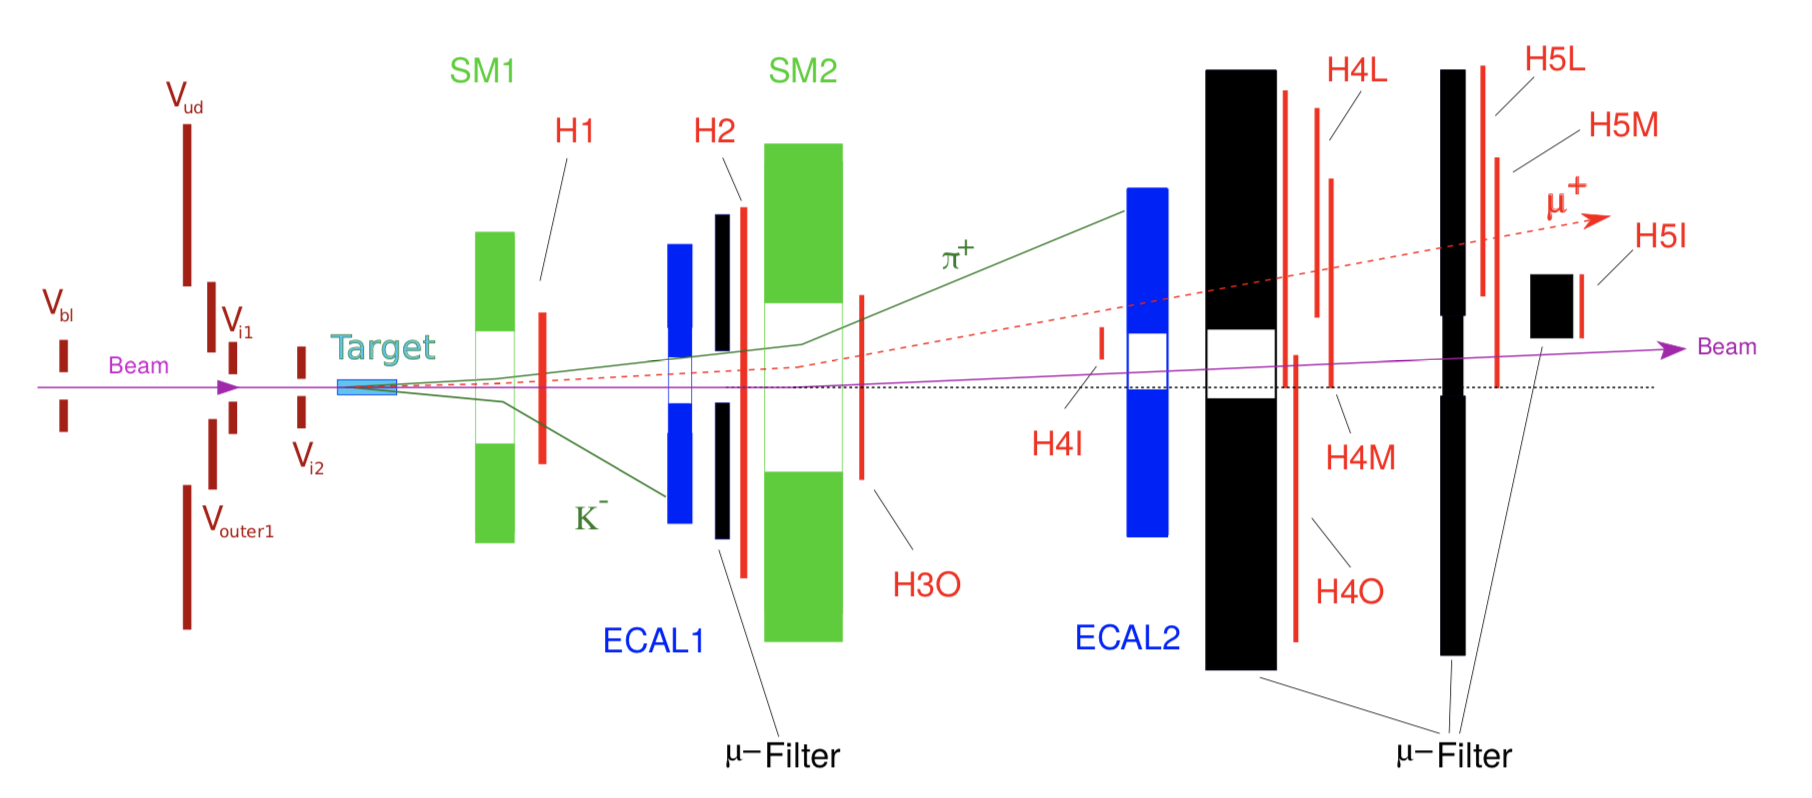
\includegraphics[scale=0.3]{./gfx/TriggerSys.png}}
  \subfloat[]{\includegraphics[scale=0.26]{./gfx/TriggerCov.png}}
	\caption{(a) Main elements of the trigger system. (b) Trigger system kinematic coverage.}
	\label{pic:trigger}
\end{figure}

%----------------------------------------------------------------------------------------

\section{Data Acquisition}

The data acquisition system (DAQ) \cite{NIM} is in charge of managing the information coming from more than $250000$ spectrometer electronic channels and building events. At COMPASS the typical event size is $45$ kB at a trigger rate of about $10$ kHz. The pipeline used in the DAQ is illustred in Fig.~\ref{pic:DAQ}. First the analog signals are coming from the detectors are preamplified, then they are digitized directly at the front-end by Analog to Digital Converters (ADCs) or Time to Digital Converters (TDCs) according to the type of detectors the front-ends are coupled to. The data are then transferred to the readout driver modules CATCH (COMPASS Accumulate, Transfer and Control Hardware) of GeSiCA (GEM and Silicon Control and Acquisition) upon the arrival of a trigger signal provided by the Trigger Control System (TCS). CATCH and GeSiCA combine the data from up to $16$ cards (ADC or TDC) and transmit them via an optical S-Link to the computers named \textit{Readout Buffer} (ROBs, maximum through output 160 MB/s) where they are stored in $512$ MB spill buffer cards. During the $4.8$ s of beam time the data are written to memory, during the rest of the full SPS cycle ($36$ s) they are read through a PCI interface. In this way the required bandwidth is reduce by a factor of three. The events are built by 12 event builders and are then written to multiple $1$ GB large files (chunks) labeled by the run number and their consecutive chunk number. Finally the data are transferred to the CERN central data recording facility (CASTOR).

\begin{figure}[!h]
  \centering
	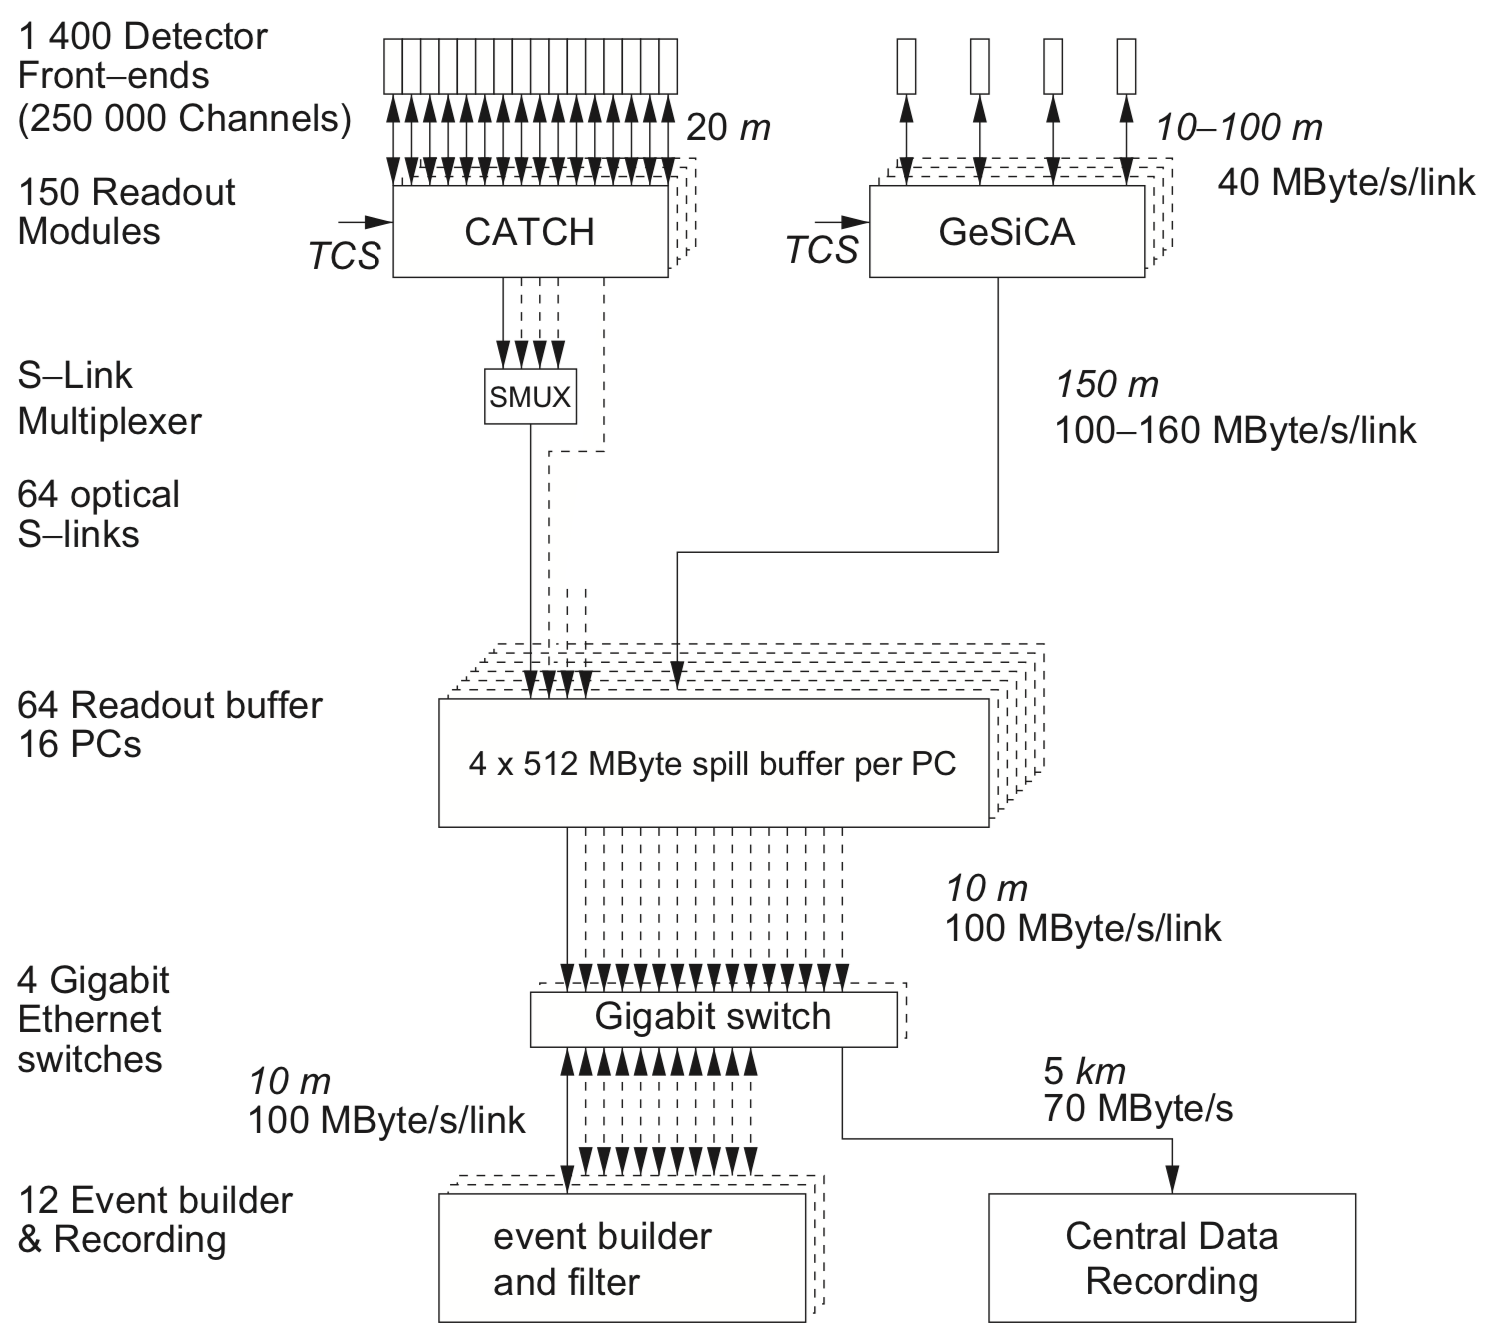
\includegraphics[scale=0.4]{./gfx/DAQ.png}
	\caption{General architecture of the DAQ system. Digitized data from the detector front-end are combined on the CATCH and GeSiCA modules. The storage of the data during the spill and the event building is performed locally. The data are recorded at the CERN computing center. Taken from \cite{NIM}.}
	\label{pic:DAQ}
\end{figure}

%----------------------------------------------------------------------------------------

\section{Event Reconstruction}

The offline reconstruction of the events stored in CASTOR is performed by the COMPASS software CORAL\footnote{COMPASS Reconstruction Algorithm Library} \cite{NIM}. CORAL is also used for the reconstruction of events generated by the Monte-Carlo simulation tool TGEANT (see Chapter~\ref{ch:MC}). CORAL is written in C++ and has a modular structure. The scheme of the steps followed by the reconstruction program is shown in Fig.~\ref{pic:CORAL}. First the information on the fired detectors channels is extracted. This is known as decoding and in the MC case digitization. In general there are more than one detector channels fired by the same particle. In that case a clustering algorithm is applied : the neighbouring detector channels that were fired are grouped together and the coordinate of the cluster in the apparatus reference system is computed. At this stage the detector calibration and position are used to extract the information. The CORAL output is stored in a ROOT Tree called mDST (mini Data Summary Tape).

The physics information is extracted from the mDST using the software package PHAST\footnote{PHysics Analysis Software Tools}. PHAST gives access to the reconstructed event information and it provides a set of algorithm to compute the relevant physics variables of each event. The PHAST outputs are stored again in a ROOT Tree. These files are significantly smaller than the mDSTs and are used for the final physics analysis.

In COMPASS, the experimental data are organized into several levels. The basic level are the events collected in one \textit{spill} provided by the SPS. A \textit{run} is the equivalent of $200$ spills. As there are machine development and/or realignment each week, the data are then structured in \textit{weeks} (also called \textit{period}) containing multiple runs.

\begin{figure}[!h]
  \centering
	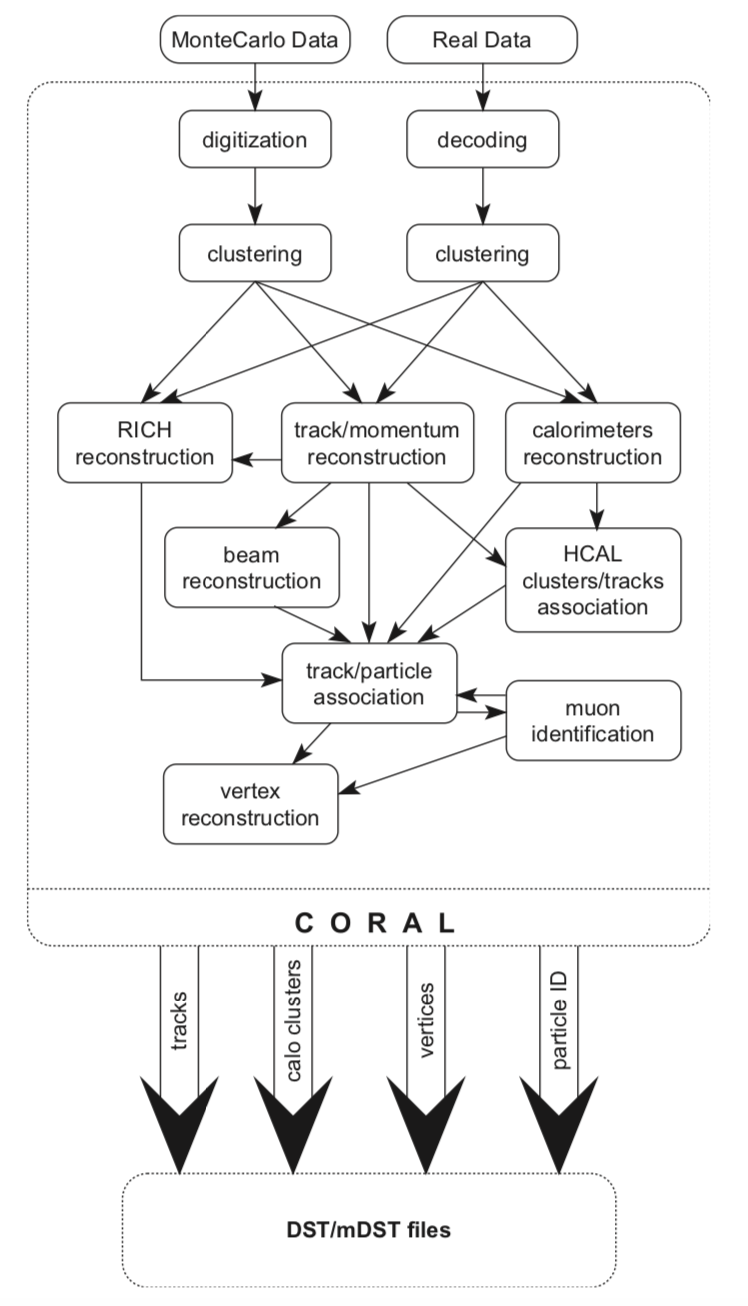
\includegraphics[scale=0.55]{./gfx/CORAL.png}
	\caption{Schematic representation of the COMPASS reconstruction software. Taken from \cite{NIM}.}
	\label{pic:CORAL}
\end{figure}
 % The COMPASS experiment
% Chapter 4

\chapter{RICH Detector}
\label{ch:RICH} % For referencing the chapter elsewhere, use \autoref{ch:name}

%----------------------------------------------------------------------------------------

The particle identification is an important step in the hadron multiplicity extraction. In the COMPASS spectrometer it is performed by a large Ring Imaging Cherenkov detector (RICH) capable of separating pions, kaons and protons in a wide momentum range ( $\sim$$2$ GeV/$c$ to $\sim$$55$ GeV/$c$) and an angular aperture of $0.01$-$0.4$ radians.

In this chapter the RICH detection principle is presented as well as the description of its main components: the gas and mirror system, the photon detectors, the readout electronics and the data reconstruction.

\section{Cherenkov effect}

When a charged particle is moving through a transparent medium with a speed v greater than the speed of light (v$_{light} = c/n$, $n$ being the medium refractive index), a radiation known as \textit{Cherenkov radiation} is produced by the medium.

\begin{figure}[!h]
  \centering
	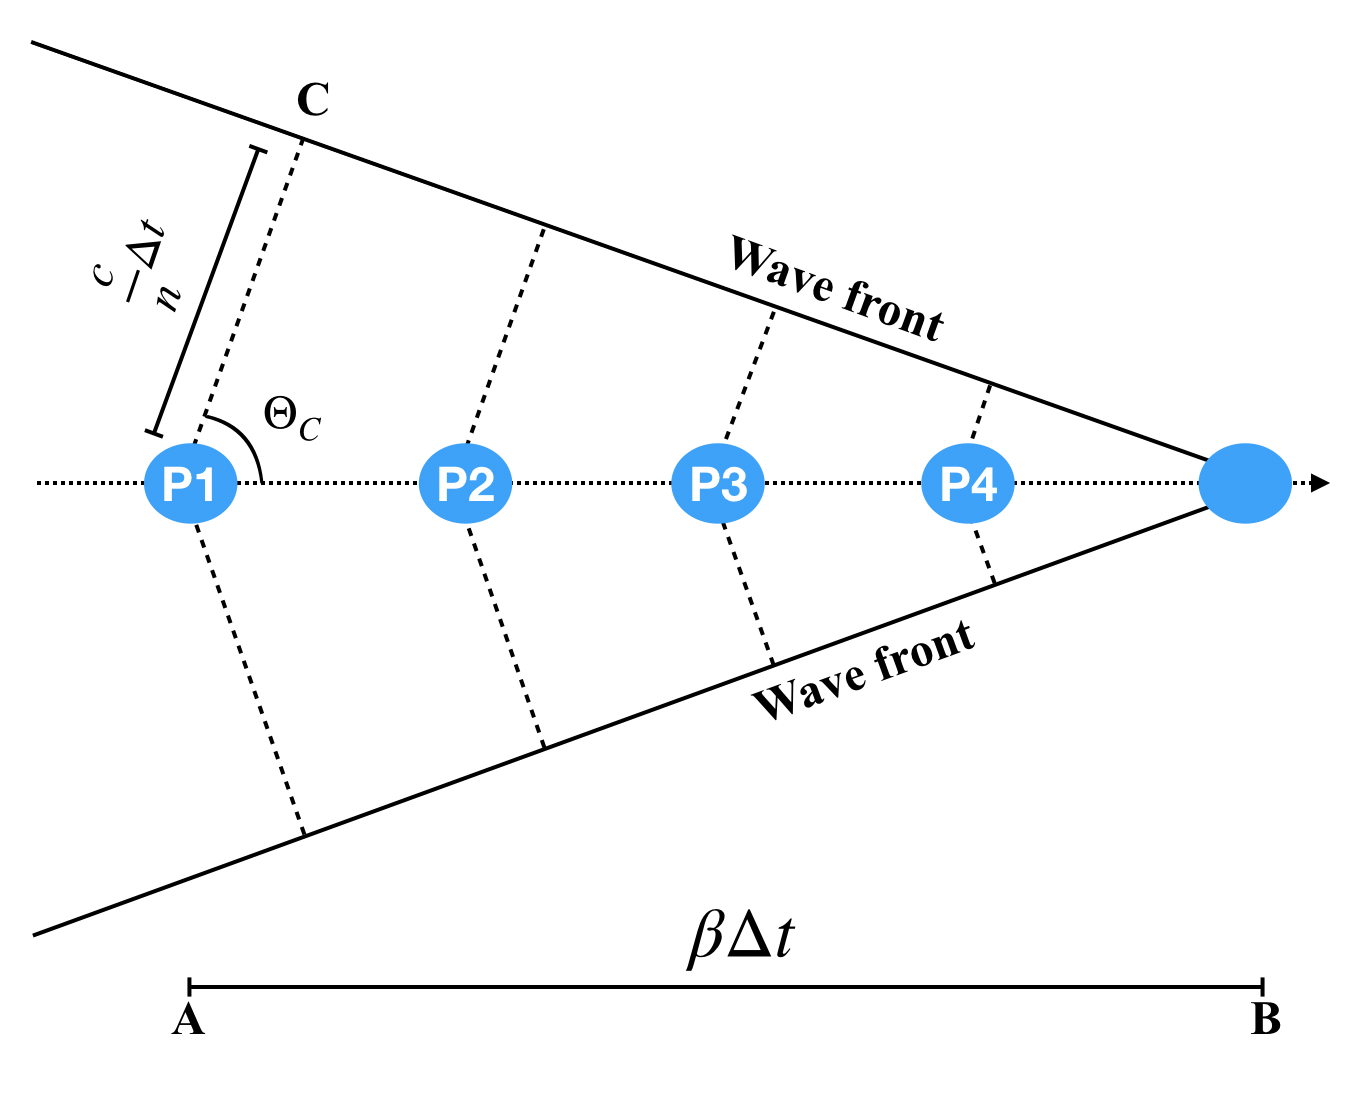
\includegraphics[scale=0.5]{./gfx/CherenkovGeom.png}
	\caption{Cherenkov radiation geometry.}
	\label{pic:CherenkovGeom}
\end{figure}

The Cherenkov radiation produced by a particle with a mass $M_h$ and momentum $p_h$ is emitted in a narrow cone around a particular angle $\Theta_C$ with respect to the particle track (Fig.~\ref{pic:CherenkovGeom}). The wavelength of these radiations goes from visible to UV.

The coherence between waves (emitted between A and B) is achieved, when the particle traverses $\overline{AB}$ at the same time as the radiation travels from A to C. The opening angle $\Theta_C$ is defined geometrically in Eq.~\ref{eq:thetaC} with $\beta$ being the particle velocity over the speed of light.
%
\begin{equation}
  cos\Theta_C = \frac{c/n \Delta t}{\beta c \Delta t} = \frac{1}{n\beta}
  \label{eq:thetaC}
\end{equation}
%
Some limit cases can be devised:
\begin{enumerate}
  \item Threshold limit: if $\beta \leq 1/n$ no Cherenkov radiation will be emitted.
  \item Maximum emission angle: $cos \Theta_C = \frac{1}{n}$ is reached for ultra-relativistic particles ($\beta = 1$).
\end{enumerate}

In order to perform particle identification with a RICH detector, two variables have to be measured: $\Theta_C$ and $p_h$. The angle can be measured detecting the emitted photons. Different techniques can be used to collect and transport the produced photons to the location of the light detectors. The resulting image in the detector plane is a ring, only for specific techniques, if one does a proper optical image. In such a case the ring has a radius proportional to $\Theta_C$. $p_h$ is measured independently by the spectrometer. The particle mass can thus be calculated by:
%
\begin{equation}
  M_h = p_h \sqrt{n^2 cos^2 \Theta_C -1}
\end{equation}

%------------------------------------------------

\section{The COMPASS RICH detector}

The COMPASS RICH detector is designed to distinguish between pions, kaons and protons at high intensities. The momentum range covers the pion Cherenkov threshold ($\sim$ $2.67$ GeV/c) to $\sim$ $55$ GeV/c.

The RICH is a large size detector ($\sim$ $3$ x $5$ x $6$ m$^3$, see Fig.~\ref{pic:RICHview}) filled with a gaseous radiator. Two spherical mirror systems reflect the photons into an array of photon detectors sensitive to a large wavelength range, from visible to far UV, placed outside the spectrometer acceptance, one above and one below the beam line. The goal is to count as many photons as possible with a good spacial resolution. The whole structure of the detector vessel is built mainly in thin aluminium in order to minimize the material budget.

Until $2004$, MultiWire Proportional Chambers (MWPC) equipped with solid-state CsI photo-cathodes were used to detect Cherenkov photons. The gains of the MWPC operation was limited. The first stage of the electronic readout was characterized by a long integration time, which was a limiting factor in the COMPASS environment as there is a high-rate uncorrelated background due to the large muon halo beam. Moreover, the long base-line restoration time generated a non-negligible dead time. To overcome these limitations, the central region that covers $25$\% of the photo-detection surface was replaced with MultiAnode PhotoMultiplier Tubes (MAPMT). They are intrisically fast and have better time resolutions.

\begin{figure}[!h]
  \centering
	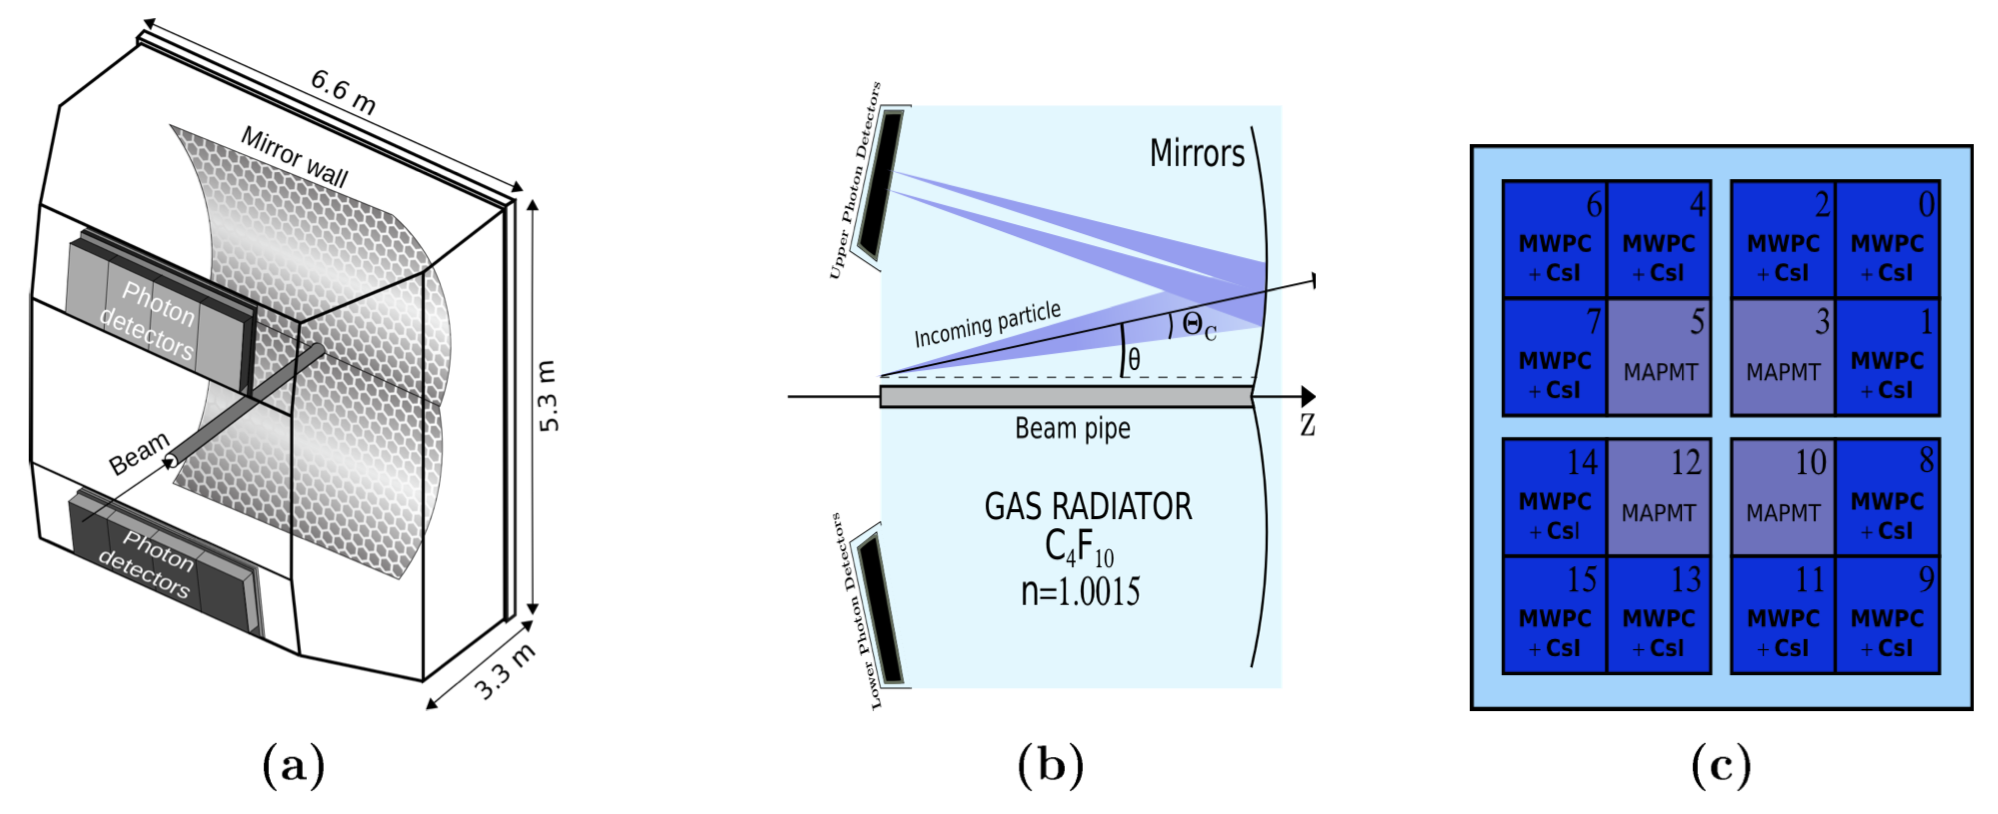
\includegraphics[scale=0.4]{./gfx/RICHview.png}
	\caption{(a) Artistic view of the COMPASS RICH detector. (b) Basic functioning of the RICH detector. (c) Photon detector disposition (not to scale).}
	\label{pic:RICHview}
\end{figure}

\subsection{Gas System}

One of the principal elements of a RICH detector is the radiator. At COMPASS it is perfluorobutane (C$_4$F$_{10}$). It has a refractive index of n $\approx$ $1.0015$ and a low chromaticity\footnote{Dependence of the refractive index of a dielectric medium on the photon wavelength \cite{Dispersion}} ($dn/dE_{\gamma}$ of about $5 \cdot 10^{-5}$~eV$^{-1}$). These characteristics allow the particle identification (PID) to be performed in the aforementioned wide momentum range.

The propagation of the Cherenkov photons in the vessel can be affected by the presence of water vapor and oxygen (high UV light absorption cross section). In order to remove these impurities, the gas is constantly circulating and filtered at a constant pressure (1 mbar higher than the atmospheric pressure) in a dedicated gas system \cite{RICHGas}. The overpressure of the vessel is needed to prevent air contamination and to avoid mechanical stress to the detector, given its large size. Other circulation system (known as \textit{fast circulation} system) allows a reshuffling of the gas inside the vessel: as perfluorobutane has a density of $11.21$ kg/m$^3$ it avoids stratification that may cause a gradient in the value of the refractive index from top to bottom.

In order to absorb the photon emitted by the muon beam, a $10$ cm diameter pipe filled with helium is positioned inside the vessel along the beam.

\subsection{Mirror System}

The RICH optical system covers an area of $\sim$ $21$ m$^2$ and consists of two spherical surfaces, each one containing $58$ spherical mirrors of different shapes ($34$ hexagons and $24$ pentagons). The mirror pattern is shown in Fig.~\ref{pic:RICHmirrors}. All the mirrors have a reflectance above $80$\% in the UV region.

The mirror system has a radius of curvature of $6.6$ m. The photon image is focused outside the spectrometer acceptance where the photon detectors are located. As the radii of the curvature have a scatter of $1$\% (R = $6600\pm66$ mm), the reflected image is slightly blurred. This effect is more pronounced for particles at large angles \cite{RICHMirror}: this aberration contributes to the dispersion of the photon angle with respect to the angle of emission, which affects the detection resolution \cite{RICHPID}.

\begin{figure}[!h]
  \centering
	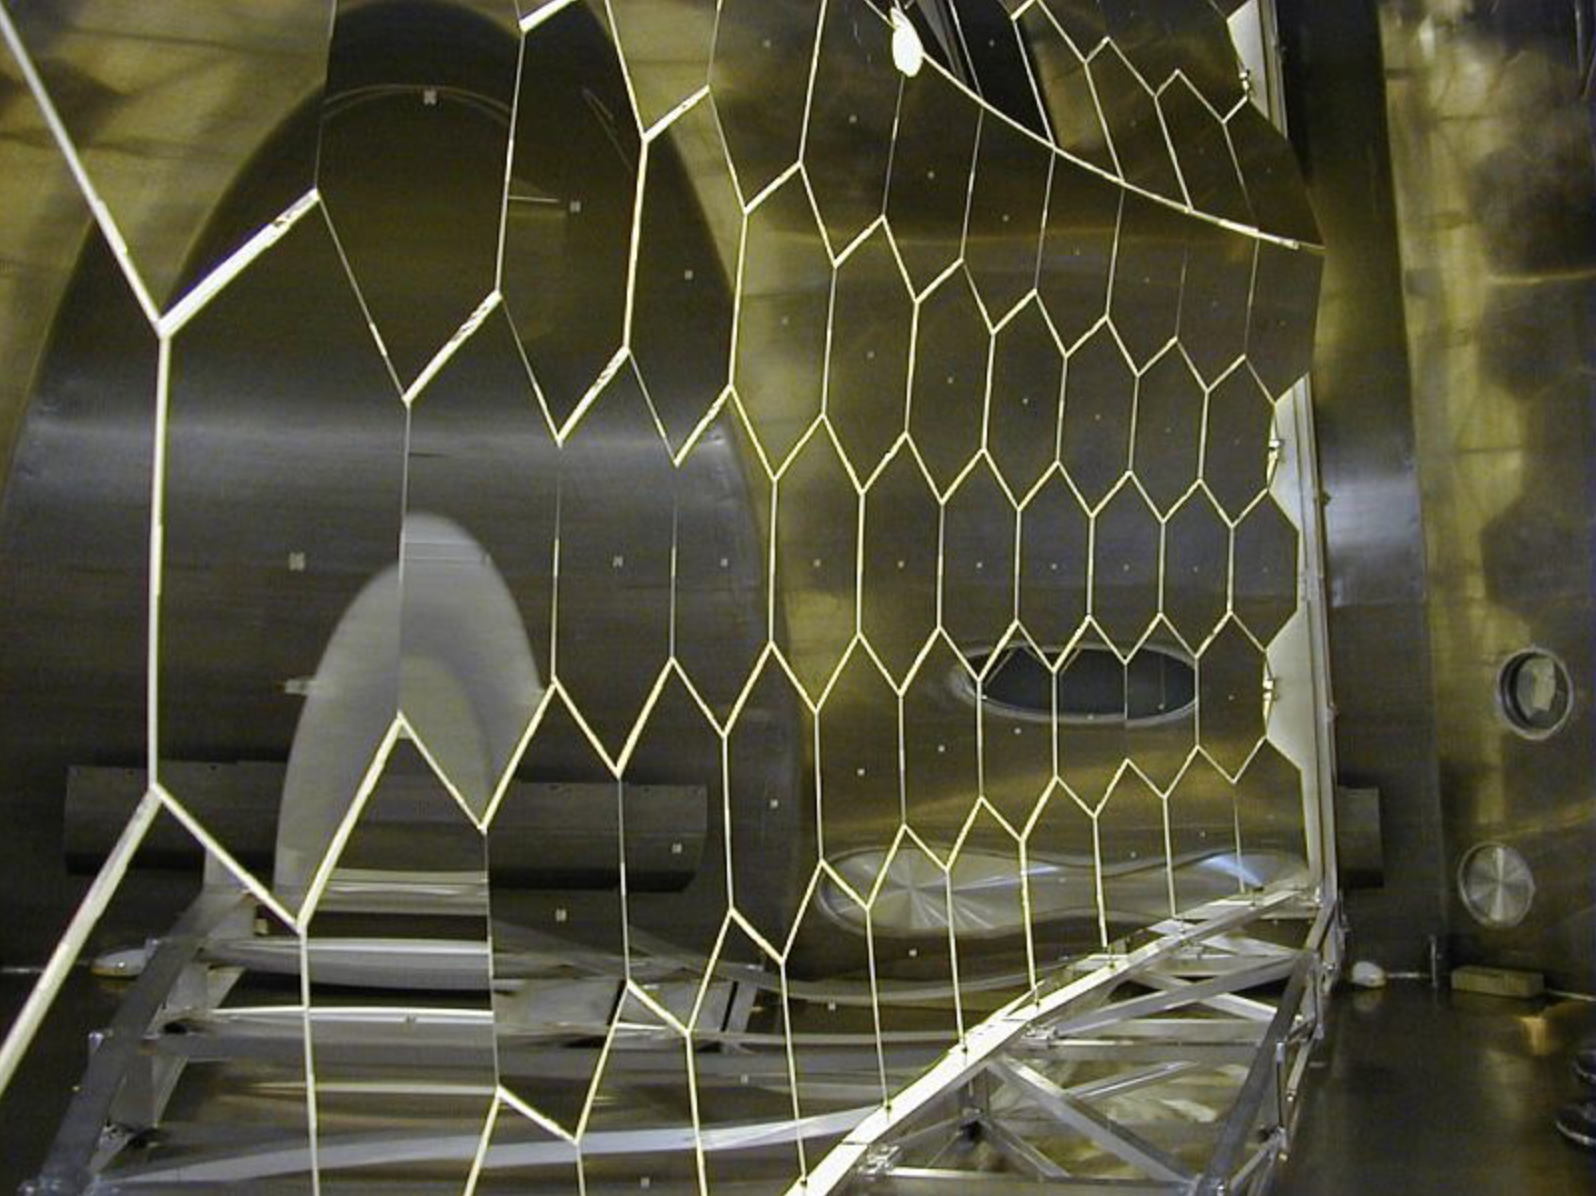
\includegraphics[scale=0.4]{./gfx/RICHmirrors.png}
	\caption{COMPASS RICH detector optical system.}
	\label{pic:RICHmirrors}
\end{figure}

\subsection{Photon Detectors}

The photon detector array consists of two symmetric parts with respect to the beam line, each one is composed of $8$ modules located at the mirror focal plane. The modules in the external regions are MultiWire Proportional Chambers (MWPC) equipped with solid state CsI photo-cathodes \cite{RICHLimits}. The central area is composed by MultiAnode Photomultiplier Tubes (MAPMT) \cite{RICHUpgrade} coupled to individual telescopes of fused silica lenses. The use of two different detector types employing different different photon converters results in the detection of photons in two wavelength regions: < $200$ nm for MWPCs and $\sim$ $200$ - $650$ nm for MAPMT. The low momentum particles are mainly detected by the outer part (MWPC), while the high momentum ones are detected by the central part (MAPMT). Only the central part is used in the following analysis.

The spherical mirrors will focus all the photons emitted parallel in the same point. Thus the Cherenkov light cone of our particle will result in a ring at the detector plane. The distribution of photons in the detectors for a physics event is shown in Fig.~\ref{pic:RICHEvent}.

\begin{figure}[!h]
  \centering
	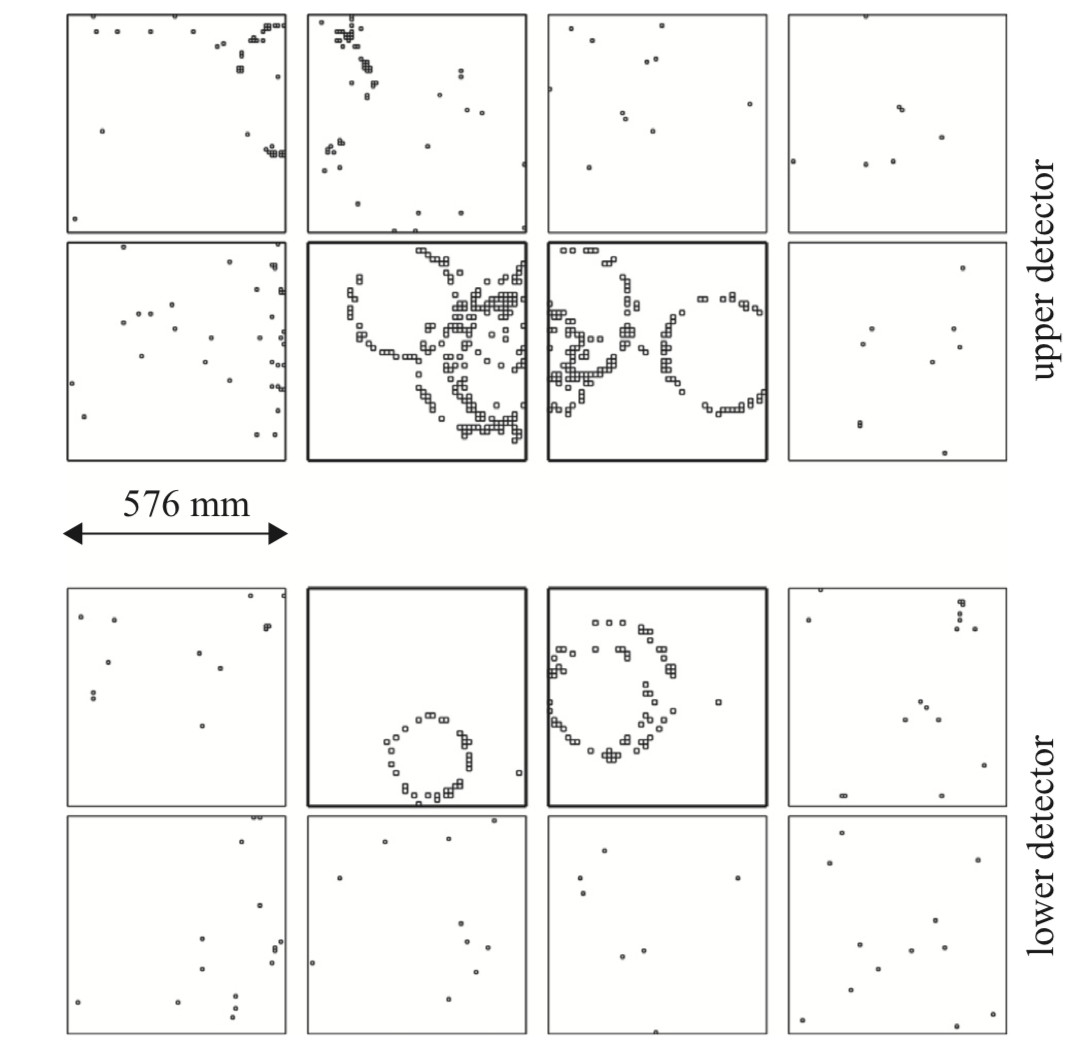
\includegraphics[scale=0.5]{./gfx/RICHEvent.png}
	\caption{An event from the online event display of COMPASS RICHONE. The $16$ squares represent the detectors areas ; the four central ones are equipped with MAPMTs. the small squares represent the hits with signal amplitudes larger than a threshold, individually set for each channel. Figure taken from \cite{NIM2015}}
	\label{pic:RICHEvent}
\end{figure}

\subsection{RICH Infos Reconstruction}

RICHONE is a package contained in the CORAL software, which is in charge of RICH information reconstruction. The reconstruction is divided in several parts, the first being decoding the data and clustering. Then the reconstruction of the Cherenkov angle for each individual photon is done. It is possible to perform a ring reconstruction which is used for studies on the apparatus. The particle identification (PID) is based on a maximum likelihood calculation. The PID will be explained more thouroughly afterwards.

\subsubsection*{Decoding and clustering}

There are two different types of photon detectors and they have different decoding systems and clustering algorithms. For the MWPCs, if more than one channel fires, a clustering is done. When the pad with the highest pulse height is found, all the adjacent pads with a smaller signal are included in the cluster \cite{RICHPID}. The mean position of each active pad is evaluated in the cluster, weighting the signal with their maximum pulse height, to determine the center of gravity of the cluster. For the MAPMT, decoding the signal is enough to read the time information coming from the PMT that was hit. As the probability of having correlated hits in adjacent area is negligible, the MAPMT data does not need clustering \cite{RICHElec}.

The cluster or hit position is used to determine the trajectory of the photon. In addition, the time information coming from the MAPMT is used to reject out-of-time photons while the amplitude information from the MWPC serves to reduce the background both from out-of-time photons and from electronic noise \cite{RICHPID}.

\subsubsection*{Cherenkov angle and ring reconstruction}

The ring reconstruction begins with the selection of a particle tracks. Then one looks for the photons around this track. The trajectory of each Cherenkov photon is calculated with respect to the plane containing the particle track and its virtual reflection in the mirror in order to reconstruct $\Theta_C$ \cite{RICHTheory}. All the photons emitted by one particle are expected to have the same angle $\Theta_C$ and to be uniformly distributed in $\phi$. The photons emitted by other particles or from background have on the contrary a flat $\Theta_C$ distribution. The emitted photon with the same ($\Theta_C$,$\phi$) pair are reflected on the same location at the focal surface (neglecting any spherical aberration), resulting in a ring image of the photon detector. Since the emission point of the photon along the particle trajectory is not known, the middle point between the detector and the mirror is taken. A good determination of the track trajectory parameters and the momentum of the particle are mandatory in order to extract $\Theta_C$ with good precision.

To characterize the RICH, determining its angular resolution for instance, the ring reconstruction of the emitted photons is needed. The ring reconstruction is based on the search of a peak in the $\Theta_C$ distribution. Small intervals of $\pm$3$\sigma$ ($\sigma$ being the single photon resolution, $\sigma_{MAPMT}$ = $2.0$ mrad and $\sigma_{MWPC}$ = $2.5$ mrad) on an overall range of $0$ to $70$ mrad are considered. The interval with the maximum number of entries is used to define the ring. This procedure associates a ring to each track and in order to reject tracks with only background photons a minimal amount of photons per ring is required (four photons for the MAPMT part) \cite{RICHPID}. The resolution of the Cherenkov angle measurement provided by each single photon as a function of the particle momentum is illustrated in Fig.~\ref{pic:RICHRez}.

\begin{figure}[!h]
  \centering
	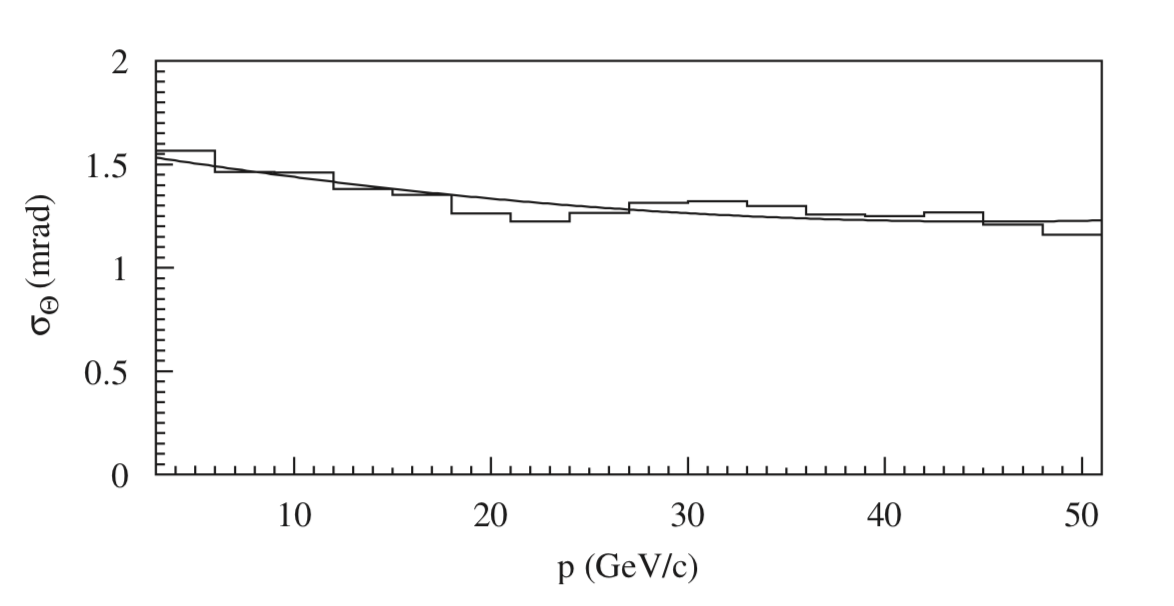
\includegraphics[scale=0.5]{./gfx/RICHRez.png}
	\caption{Resolution of the Cherenkov angle for the reconstructed ring images, provided by each single photon, versus the particle momentum for a sample of identified pions. Figure taken from \cite{NIM}.}
	\label{pic:RICHRez}
\end{figure}

The measured values of $\theta_C$ as a function of $p_h$ for the RICH detector are shown in Fig.~\ref{pic:RICH}. In the low momentum region, the RICH detector is only sensitive to electrons, muons and pions. The bands corresponding to kaons and protons start to be visible respectively at $p_h \approx$ $9.45$ GeV/c and $p_h \approx$ $17.95$ GeV/c. For high momentum values above $40$ GeV/c, saturation of the Cherenkov angle is observed or pions and kaons. The final particle identification is performed using likelihood methods and is described in the following chapter.

\begin{figure}[!h]
  \centering
	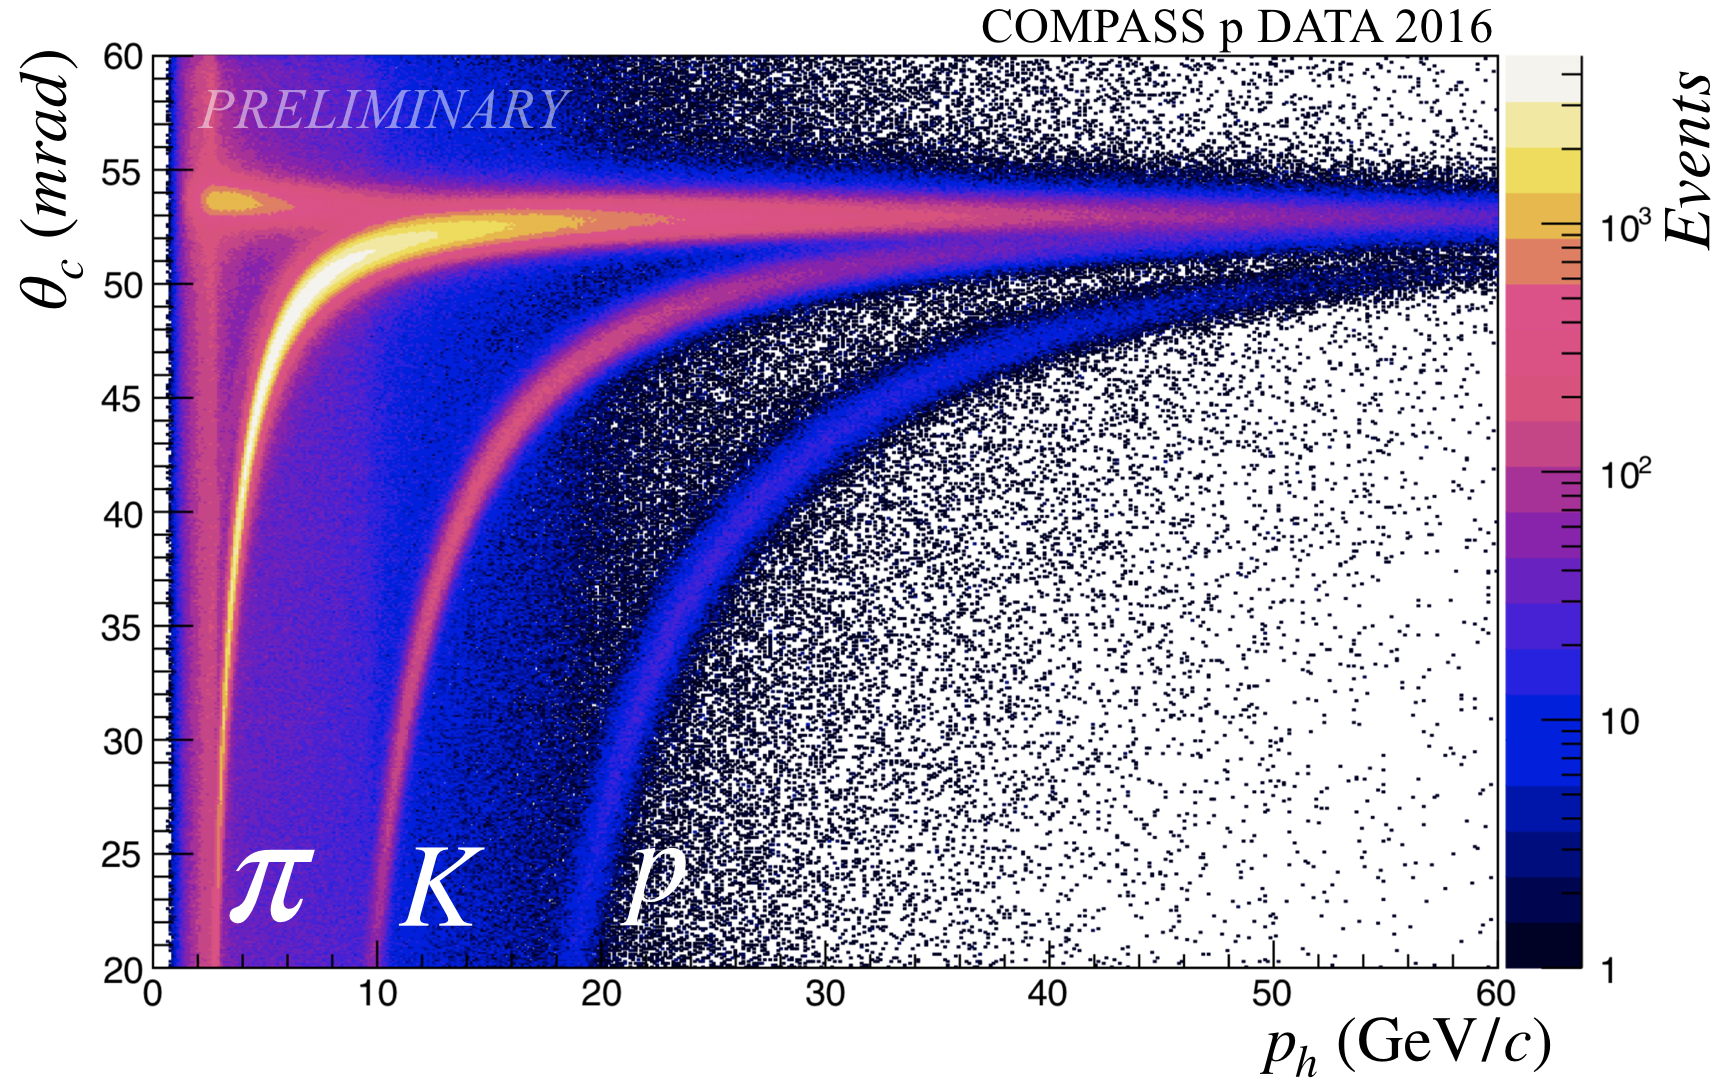
\includegraphics[scale=0.45]{./gfx/RICH.png}
	\caption{Measured Cherenkov angle $\Theta_C$ as a function of $p_h$. $\pi$ threshold is about $2.67$ GeV/$c$, $K$ threshold about $9.45$ GeV/$c$ and $p$ threshold about $17.95$ GeV/$c$, respectively.}
	\label{pic:RICH}
\end{figure}
 % The COMPASS RICH
% Chapter 5

\chapter{Performance Study and Particle Identification}
\label{ch:PID} % For referencing the chapter elsewhere, use \autoref{ch:name}

%----------------------------------------------------------------------------------------

For particle tracks with a measured momentum using the RICH information enables us to determine the particle mass and thus identify the particle. As the detector efficiency is not perfect, the misidentification probability is not zero ; one thus has to determine the identification performance of the RICH detector. The RICH performance study relies on extracting the identification and misidentification probabilities for pions, kaons and protons. From samples of pure pions, kaons and protons the RICH detector response is measured: the hadrons are identified using RICH information and the identification and misidentification probabilities are calculated in the hadron ($p_h$,$\theta_h$) phase space for pions, kaons and protons. The method used for identification is a likelihood estimation for different hypotheses. At first order, the mass assignment corresponds to the highest likelihood, but further requirements can be added to improve the result.

\section{Determination of RICH Detector Performance}

The identification and misidentification efficiency is given by the ratio of the number of particles correctly and wrongly identified, respectively, out of a pure sample of specific hadron type species over the total number of hadrons composing the pure sample:

\begin{equation}
    \epsilon(t \rightarrow i) = \frac{N(t \rightarrow i)}{N(t)}
\end{equation}

$\epsilon(t \rightarrow i)$ is the probability that a particle $t$ is identified as a particle $i$, $N(t \rightarrow i)$ is the number of particles $t$ identified as $i$ and $N(t)$ is the total number of hadron $t$ of the pure sample. The identification ($\epsilon(t \rightarrow t)$) and misidentification ($\epsilon(t \rightarrow i)$) efficiencies are properties of the RICH and can be displayed in an efficiency matrix with the identification efficiencies on the diagonal and the misidentification ones off-diagonal:

\begin{equation}
  M_R
  =
  \begin{bmatrix}
  \epsilon(\pi \rightarrow \pi) & \epsilon(K \rightarrow \pi) & \epsilon(p \rightarrow \pi)\\
  \epsilon(\pi \rightarrow K) & \epsilon(K \rightarrow K) & \epsilon(p \rightarrow K) \\
  \epsilon(\pi \rightarrow p) & \epsilon(K \rightarrow p) & \epsilon(p \rightarrow p)
  \end{bmatrix}.
\end{equation}

\subsection{Selection of $\Phi$, $K^0$ and $\Lambda$}

To obtain the efficiency matrix, three pure hadron samples are needed. The RICH performance analysis is based on the study of the pion, kaon and proton samples originating from $\Phi$, $K^0$ and $\Lambda$ decays.

For the determination of the RICH efficiency, it is necessary to have a source of events where the true kind of the particle passing the RICH is known. That kind of events is obtained using two body particle decays, namely the decay of a $K^0$ into two pions ($K^0 \rightarrow \pi^+\pi^-$), the $\Phi$ decay into two kaons ($\Phi \rightarrow K^+K^-$), the $\Lambda$ decay into a pion and a proton ($\Lambda \rightarrow p\pi^-$). In order to select events with such decays, scattering events with a scattered muon are selected. The following cuts are thus applied to the data:
\begin{itemize}
  \item Exclude bad spills
  \item Select best primary vertex with incoming and scattered muon
  \item Check if primary vertex is inside one of the target cells
  \item Extrapolated track of the incoming muon should cross all target cells
  \item $0.1 \le y \le 0.9$
\end{itemize}

Different selection criteria have to be used for $K^0$, $\Lambda$ and $\Phi$ decays. In the case of $K^0$ mesons and $\Lambda$ baryons, the particles decay by the weak force. Therefore, the decay length is long enough to produce a secondary vertex, which can be separated from the primary one. The $\Phi$ mesons decays by the strong force. This results in a very short decay length and it is not possible to separate the secondary vertex from the primary one.

\subsection{$K^0$ and $\Lambda$ selection}

For $K^0$ mesons the decay into $\pi^+$ and $\pi^-$ with a branching ration of ($69.20$~$\pm$~$0.05$)\% \cite{PDG} and in the case of $\Lambda$ and $\bar{\Lambda}$ baryons the decay into a proton and a pion with a branching ratio of ($63.9$~$\pm$~$0.5$)\% \cite{PDG} is used. In both decays the reconstruction of the secondary vertex is possible. The following cuts are applied to select these decays:

\begin{enumerate}
  \item Selection of good secondary vertices
  \begin{itemize}
    \item Loop over all vertices
    \item Vertex is not primary one
    \item Exactly two opposite charged outgoing particles
    \item The tracks should not be connected to any other primary vertex to ensure that they belong to a secondary vertex
    \item Primary and secondary vertex separated by more than two times the reconstruction accuracy
  \end{itemize}
  \item Select good hadron tracks
  \begin{itemize}
    \item Both particles should not have crossed more than $10$ radiation length in order to supress the muons from the sample.
    \item Last measured position ($Z_{last}$) behind SM$1$ to ensure a measured momentum
    \item Transverse momentum with respect to the mother particle larger than $23$ MeV to suppress electrons from photon conversion
    \item Check that the decaying particle is connected to the primary vertex ($\theta_p \le 0.01$)
  \end{itemize}
  \item Additional cuts
  \begin{itemize}
    \item $p_h \geq 1$ GeV/$c$
    \item Mass difference smaller than $150$ MeV/$c^2$ between the $K^0$/$\Lambda$ mass and the invariant mass of the two decay hadrons assuming the correct masses
  \end{itemize}
\end{enumerate}

The same cuts except for the mass cuts are used for $K^0$ and $\Lambda$ candidates. The transverse momentum of K, $\Lambda$ or dacay product is shown as a function of the ratio of the longitudinal momentum ratio of two particles:
%
\begin{equation}
  \alpha = \frac{p_{L,1}-p_{L,2}}{p_{L,1}+p_{L,2}},
\end{equation}
%
in the Armenteros plots in Fig.~\ref{pic:Armenteros} (a) for $K^0$ and $\Lambda$ and (b) for $\Phi$.

\begin{figure}[!h]
  \centering
	\subfloat[$K^0$ and $\Lambda$]{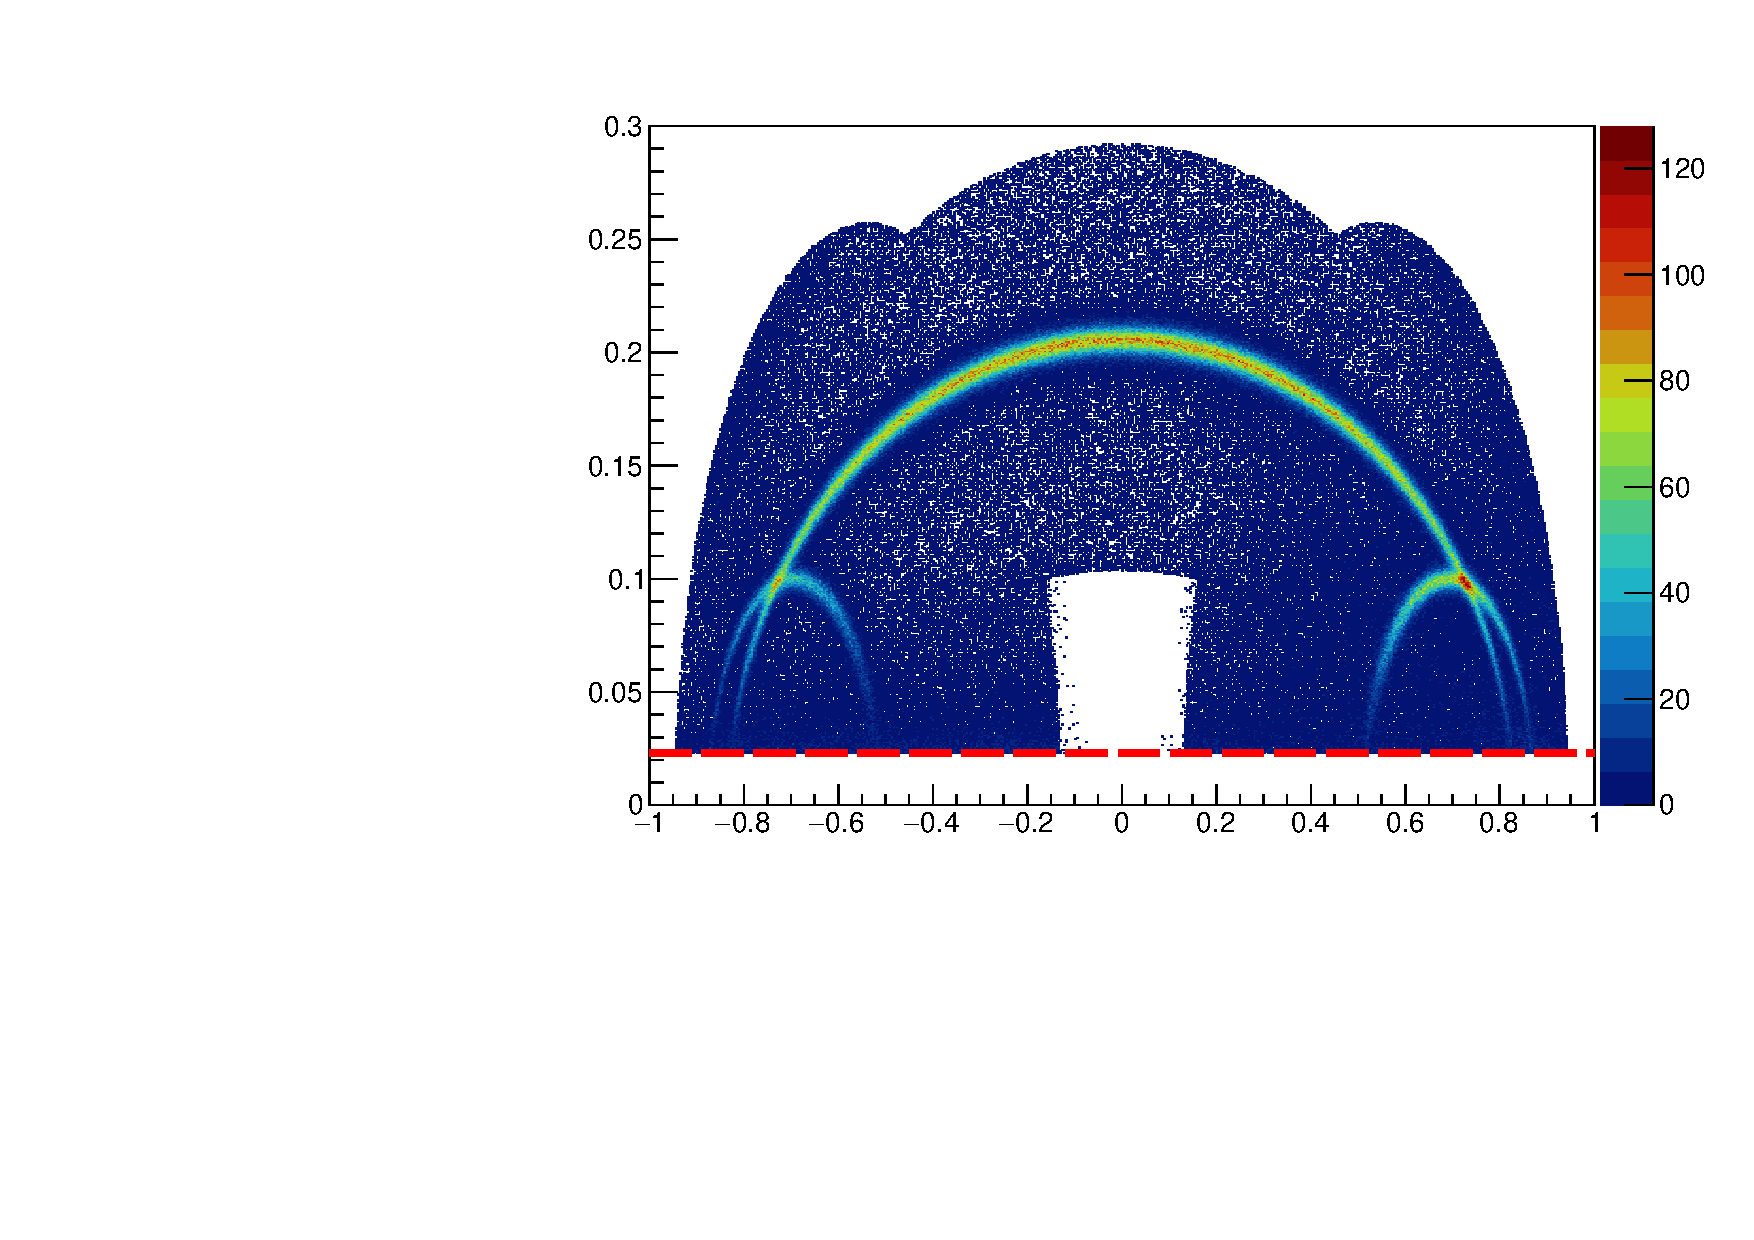
\includegraphics[scale=0.42]{./gfx/ArmenterosK0L.pdf}}
  \subfloat[$\Phi$]{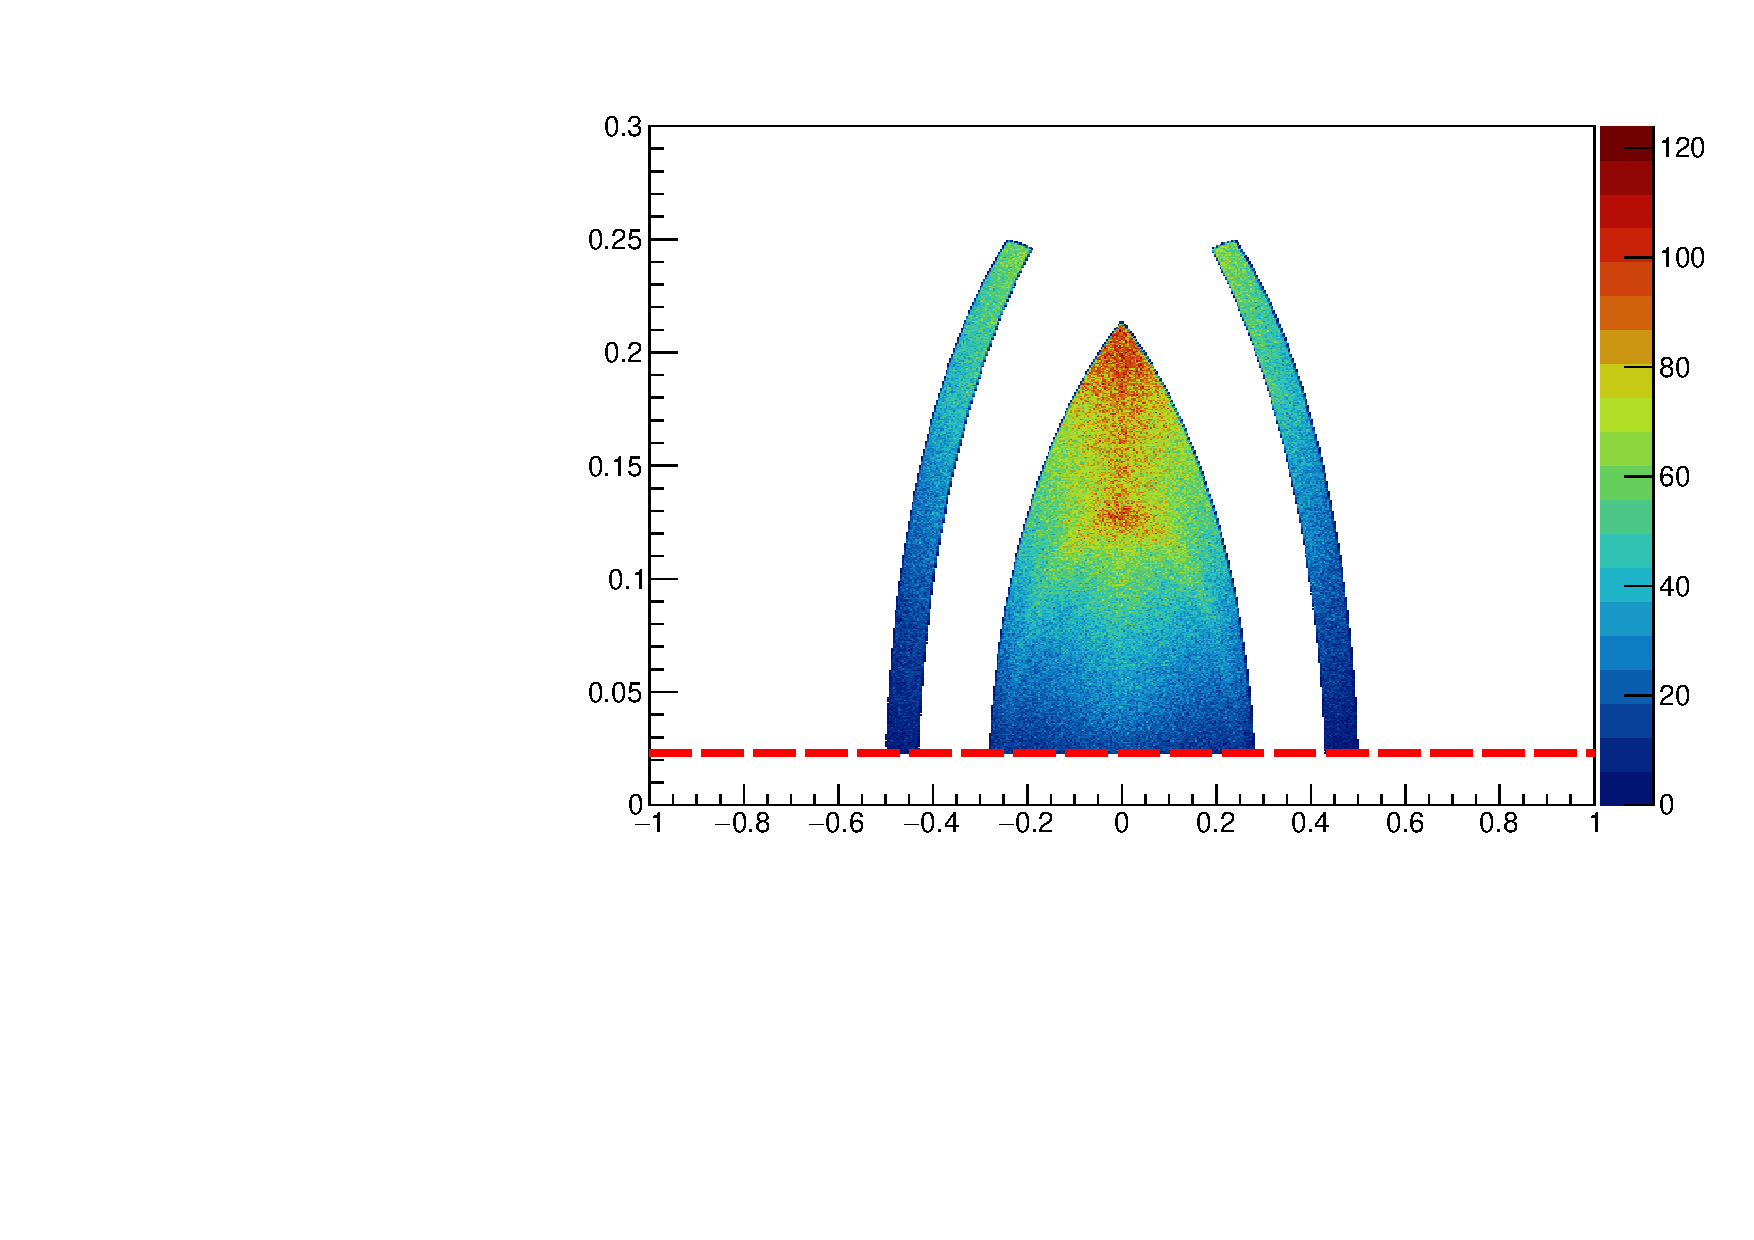
\includegraphics[scale=0.42]{./gfx/ArmenterosPhi.pdf}}
	\caption{Armenteros plots. The cut on the transverse momemtum is illustrated by the red line.}
	\label{pic:Armenteros}
\end{figure}

The three visible arcs are produced by the decay of the $K^0$ mesons and the $\Lambda$ baryons. The decay of $K^0$ mesons in two particles with the same mass results in the symmetric arc, whereas the decay of $\Lambda$ baryons into two particles with different masses result in the two smaller arcs on the left and right side. All particles below the red dashed line, which corresponds to the $23$ MeV limit, are rejected in order to supress tracks from electron coming from photon conversion.

\subsection{$\Phi$ selection}

The branching ratio of the $\Phi$ decay into two kaons is ($48.9$~$\pm$~$0.5$)\% \cite{PDG}. The $\Phi$ meson decay length is too short to separate the primary and decay vertex. Therefore, all outgoing particles from a primary vertex are taken into account for the search of possible $\Phi$ mesons. The selection steps are similar the selection of the $K^0$/$\Lambda$ candidates:

\begin{enumerate}
  \item Selection of possible good events with $\Phi$ mesons
  \begin{itemize}
    \item At least three outgoing particles including scattered muon
    \item Loop over all outgoing particles
    \item Oppositely charged pairs of hadrons (none is a muon)
  \end{itemize}
  \item Select good hadron tracks
  \begin{itemize}
    \item Last measured position ($Z_{last}$) behind SM1 to ensure a measured momentum
    \item Transverse momentum with respect to the mother particle larger than $23$ MeV to suppress electrons from photon conversion
  \end{itemize}
  \item Additional cuts
  \begin{itemize}
    \item $9$ GeV/$c$ $\leq p_h \leq 55$ GeV/$c$
    \item Mass difference smaller than $120$ MeV/c$^2$ between the $\Phi$ mass and the invariant mass of the two decay hadrons assuming the kaon mass.
  \end{itemize}
\end{enumerate}

The selection of $\Phi$ meson candidates results in a large combinatorial background. The three regions in the Armenteros plots in Fig.~\ref{pic:Armenteros} (b) are produced by the decay of the $\Phi$ mesons. The decay of $\Phi$ mesons in two particles with the same mass results in symmetric regions. All particles below the red dashed line are rejected as in the $K^0/\Lambda$ case.

\section{Likelihood method}

The likelihood (LH) method is a statistical method that can be used to find a suitable model for describing a data set or to estimate the values of the parameters used in this model \cite{LH1,LH2}.

The first step is to define the LH function. Let $\mathbf{s}$ be a sample of elements $s_i$, $i \in \llbracket 1,l \rrbracket$:
%
\begin{equation}
  \mathbf{s} = \left( s_1,s_2,..,s_l \right),
\end{equation}
%
which follows a distribution with the probability density $f(s|\theta)$. This probabilty density is determined by a set of parameters $\theta = \theta_1,..,\theta_m$. In order to fit the sample with the model some requirements must be met.

\begin{enumerate}
  \item The sample can be considered as a $l$-dimensional random variable and can be assigned a probability density $g(\mathbf{s})$:
  \begin{equation}
    g(\mathbf{s}) = g\left( s_1,s_2,..,s_l \right).
  \end{equation}
  \item The sample is random.
  \begin{enumerate}[(a)]
    \item The $s_i$ are independent:
    \begin{equation}
      g(\mathbf{s}) = g_1\left(s_1 \right) \cdot g_2\left(s_2 \right) \cdot .. \cdot g_l\left(s_l \right).
    \end{equation}
    \item Each element $s_i$ follows the probability density of the distribution:
    \begin{equation}
      g(s_i) = f(s|\theta).
    \end{equation}
  \end{enumerate}
\end{enumerate}

If these conditions are fulfilled, the LH function $L\left(s_1,..,s_l|\theta \right)$ is defined as:
%
\begin{equation}
  L\left(s_1,..,s_l|\theta \right) = \prod_{i=1}^{l} f(s_i|\theta),
\end{equation}
%
and states that the probability of occurence of the sample is equal to the product of the occurence of each element of the sample. The probability density of the sample is normalized to its domain of definition $\Omega$:
%
\begin{equation}
  \int_{\Omega} L\left(s_1,..,s_l|\theta \right) ds_1 .. ds_l = 1.
\end{equation}
%
In order to select from all possible sets of parameters in the parameter space $\Theta$ the estimator $\hat{\theta}$, which gives the best description of the true description, one applies the Maximum Likelihood Estimation (MLE) method. The method can be formulated as follows:
%
\begin{equation}
  \hat{\theta} \in \left \{ \underset{\theta \in \Theta}{arg\,max}\,L\left(s_1,..,s_l|\theta \right) \right \},
\end{equation}
%
if a maximum exists. This means that the maximum of the LH function has to be found in relation to the parameters. Having found the maximum, one has also found the best estimate of the parameters. Since the LH function can yield very small values as a probability density, it is common to define the logarithmic LH function instead:
%
\begin{equation}
  \mathscr{L}\left(s_1,..,s_l|\theta \right) = \text{ln}\,L\left(s_1,..,s_l|\theta \right) = \sum_{i=1}^{l} \text{ln}\,f(s_i|\theta).
\end{equation}
%
The maximization condition for several parameters $\theta = \theta_1,..,\theta_m$ is thus:
%
\begin{equation}\label{eq:maximization}
  \frac{\delta \mathscr{L}\left(s_1,..,s_l|\delta\theta \right)}{\delta\theta_j} = \frac{\delta}{\delta\theta_j} \sum_{i=1}^{l} \text{ln}\,f(s_i|\theta) = 0 \quad for \quad \theta = \hat{\theta}.
\end{equation}
%
In many physics systems one can find geometrical or kinematic constraints such as the sum of the impulses equal to zero and the sum of the energies equal to twice the photon energy in the electron-positron annihilation in the center-of-mass system. These conditions can be used to eliminate one of the parameters of the system. However, this is often not desirable since this elimination is often only possible through complicated algorithm or the equivalent treatment of the parameters after the adaptation is no longer guaranteed. In order to consider the constraints further, they can be included in the LH functions as functions $c_{k}(\theta)(k=1,..,z_c)$, analogous to the method of Lagrange multipliers:
%
\begin{equation}
  \mathscr{L}\left(s_1,..,s_l|\delta\theta \right) = \text{ln}\, L\left(s_1,..,s_l|\theta \right) = \sum_{i=1}^{l} \text{ln}\, f(s_i|\theta) - \sum_{k=1}^{z_{c}} \lambda_k c_k(\theta)
\end{equation}
%
The overall $z_c$ Lagrange multipliers $\lambda_k$ are treated as additional parameters. Thus the $z_c$ conditions of the constraints still come to the maximization conditions in Eq.~\ref{eq:maximization}:
%
\begin{equation}
  \frac{\delta \mathscr{L}}{\delta \lambda_k} = c_k(\theta) = 0.
\end{equation}
%
Since the LH method is used not only for particle identification by the RICH detector but also for the fits to determine the RICH efficiencies, the extended Maximum Likelihood Estimation (eMLE) method is discussed further below. This method is used primarily for problems, in which the fit also supplies the number of expected events and these are to be adapted to the observed events. For example this is the case if there are $n$ events that results from a sum of several sources $n_i$. The constraint that follows is that $n = \sum_{i=1}^{j} n_i$. This condition can now be used as an additional factor in the LH function. The factor then corresponds to a Poisson distribution, which describes the probability that $n$ events are also observed at an expected value $\lambda$:
%
\begin{equation}
  L\left(s_1,..,s_l|\theta \right) = \frac{\lambda^n e^{-\lambda}}{n!} \prod_{i=1}^{n} f(s_i|\theta).
\end{equation}
%
For the logarithmic LH function follows:
%
\begin{equation}\label{eq:loglambda}
  \mathscr{L}\left(s_1,..,s_l|\theta \right) = n \,\text{ln}\, \lambda - \lambda + \sum_{i=1}^{n} \text{ln}\,f(s_i|\theta)
\end{equation}
%
The term $- \text{ln} (n!)$ is irrelevant for the following maximization and has been omitted. With the help of the following simplification:
%
\begin{equation}
  n \,\text{ln}\, \lambda + \sum_{i=1}^{n} \text{ln}\, f(s_i|\theta) =  \sum_{i=1}^{n} \left(\text{ln}\, f(s_i|\theta) + \text{ln}\, \lambda \right) = \sum_{i=1}^{n} \text{ln}\, (\lambda f(s_i|\theta)),
\end{equation}
%
is it possible to define a function $g(s_i|\theta) = \lambda f(s_i|\theta)$, which is normalized by $\lambda$:
%
\begin{equation}
  \int_{\Omega} g(s_i|\theta) ds_1 .. ds_l = \lambda \int_{\Omega} f(s_i|\theta)ds_1 .. ds_l  = \lambda.
\end{equation}
%
Thus Eq.~\ref{eq:loglambda} can be rewritten into the common form of an extended LH function:
%
\begin{equation}
  \mathscr{L}\left(s_1,..,s_l|\theta \right) = \sum_{i=1}^{n} \text{ln}\, g(s_i|\theta) - \int_{\Omega} g(s_i|\theta) ds_1 .. ds_l.
\end{equation}
%
It follows that $\mathscr{L}\left(s_1,..,s_l|\theta \right)$ becomes maximal, when the additional term equals the number of actual events $n$.

\section{RICH Particle Identification}

Particle identification using the LH method is accomplished by finding the maximum LH function value. The LH function describes the radial photon distribution. An essential step is to determine the radial photon distribution (see Fig.~\ref{pic:Photonfit} (a)) as precisely as possible. This depends on the detector geometry, the accuracy in determining the trajectory of the particle to be identified, as well as on the accuracy with which the parameters describing the photon position in the ring plane can be determined. The two parameters used are the reconstructed angles at which the photon ($Ph$) was emitted relative to the particle path $\Theta^{Ph}$ and the reconstructed azimuthal angle around the particle path $\Phi^{Ph}$ \cite{Pfit1,Pfit2,Pfit3}. The LH function for describing the photon distribution is given as:
%
\begin{equation}
  L_{N_{Ph}} = \prod_{k=1}^{N_{Ph}} \left[ (1-\epsilon) G\left(\Theta_k^{Ph},\Phi_k^{Ph} \right) + \epsilon B\left(\Theta_k^{Ph} \right) \right],
\end{equation}
%
where
%
\begin{equation}
  G\left(\Theta_k^{Ph},\Phi_k^{Ph} \right) = \frac{1}{\sqrt{2\pi} \cdot \sigma_{\theta,k}^{Ph}} e^{-\frac{1}{2}\frac{\left(\Theta_k^{Ph}-\Theta_k^{Ph} \right)^2}{\left(\sigma_{\theta,k}^{Ph} \right)^2}} \cdot \frac{\Theta_k^{Ph}}{\Theta^{M}}
\end{equation}
%
is a Gaussian distribution with which the signal (see Fig.~\ref{pic:Photonfit} (b)) can be described. The standard deviation $\sigma_{\theta}^{Ph}(\Phi_P^{Ph},\beta)$ originates from the accuracy with which the photon distribution can be determined. This in turn depends on the azimuthal photon angle ($\Phi_P^{Ph}$) in the plane of the photodetectors, which is characterized by the index $P$, and on the particle velocity relative to the speed of light $\beta$. $\Theta^M$ is the mass hypothesis for the considered particle. It is determined by the expected Cherenkov angle for a particular particle type or particle mass with $\beta$. Possible particles are electrons, pions, kaons and protons.

\begin{figure}[!h]
  \centering
	\subfloat[Photon distribution in the detector plane]{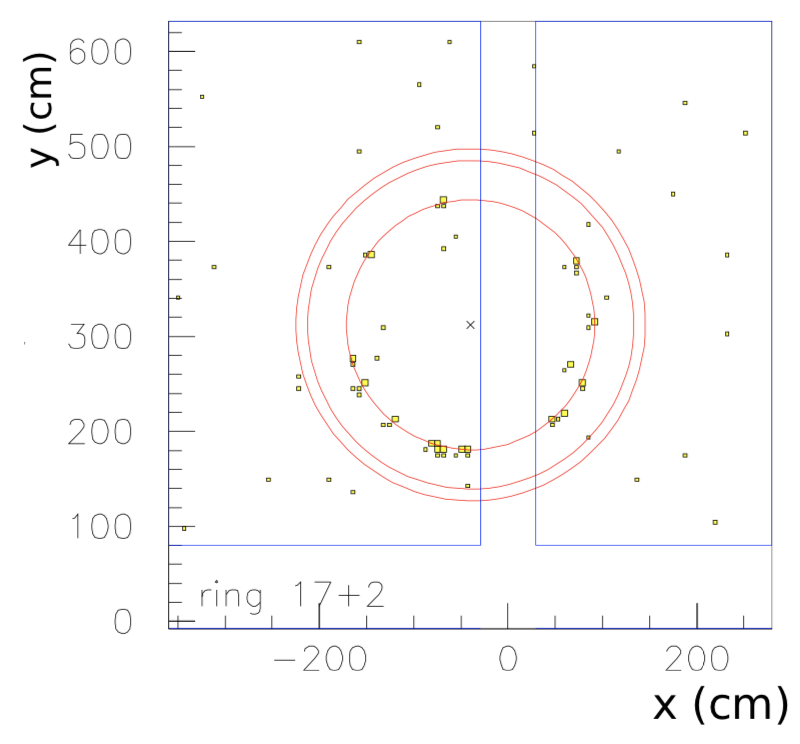
\includegraphics[scale=0.52]{./gfx/LH1.png}}
  \subfloat[LH-fit of the radial photon distribution]{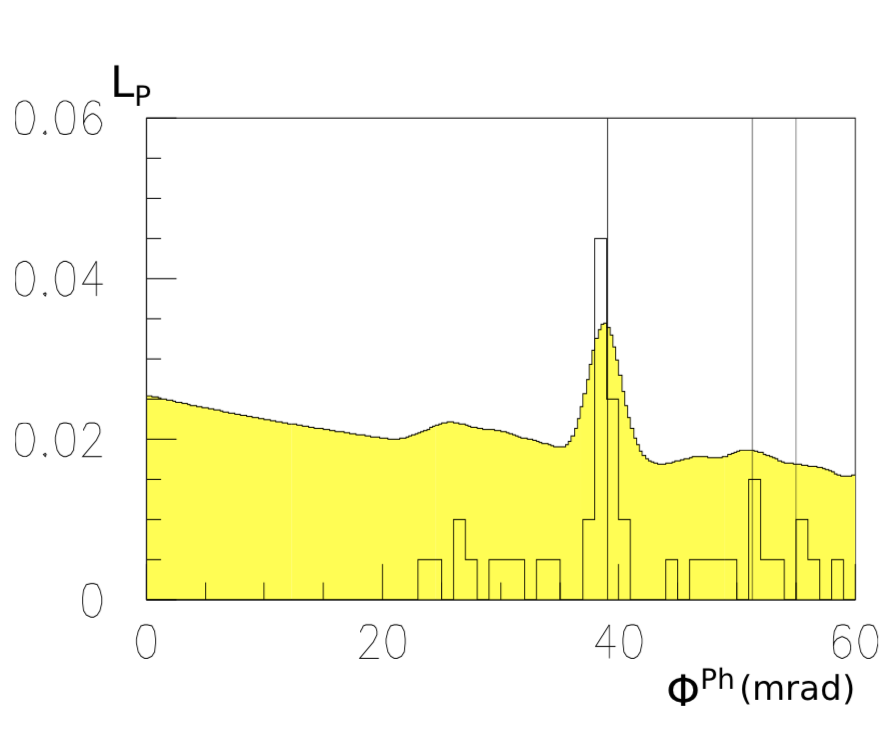
\includegraphics[scale=0.52]{./gfx/LH2.png}}
	\caption{Figure (a) shows the photon distribution in the plane of the photodetectors. The x marks the projection of the particle path. The red rings correspond, from the inside to the outside, to the distribution that would be generated by a proton, a kaon or a pion. The yellow marks are the detected photons. In (b) the result of the LH-fit of the photon distribution with the proton hypothesis is shown.}
	\label{pic:Photonfit}
\end{figure}

The RICH particle identification efficiency is studied in the momentum range of $3$ GeV/$c$ $ \leq p \leq $ $50$ GeV/$c$. In this range, pions and kaons are emitting Cherenkov light, while up to $\sim$ $17$ GeV protons are still below the threshold of:
%
\begin{equation}
  p_{thr,i} = \frac{m_i}{ \sqrt{n^{2}-1} }
\end{equation}
%
where $n$ is the refractive index. This is shown in Fig.~\ref{pic:RefIndex} where the reconstructed Cherenkov angle is shown as a function of the hadron momentum. The identification of pions, kaons and protons above the momentum threshold is done by comparing the likelihood values with one another. The identification of these particles is done using likelihood cuts. Using the likelihood values, the particle identification is done by comparing these values with one another. In the simplest case, the highest one determines the particle type. This method is used in the case of pions. In the case of kaons, stricter likelihood cuts are applied to suppress misidentified pions as the goal of the selection is to obtain a clean pion and kaon sample.  The likelihood cuts for protons require its likelihood to be the largest one.  Below the momentum threshold, protons do not emit Cherenkov light. Therefore, the likelihood values are used to test, whether the detected light is consistent with random noise in the detector (background). In order to avoid possible problems due to the uncertainty on the reconstructed momentum or the uncertainty of the refractive index of the RICH gas, a region of $\pm$ $5$ GeV/$c$ around the proton threshold is used, where both hypothesis are applied for proton identification. The likelihood cuts are listed in Table~\ref{tab:LHcut}. As the electrons cannot be distinguished from pions for momentum above $8$ GeV, they are not separated at this stage of the analysis. This contamination is dealt with the Monte-Carlo later in the analysis (Chapter~\ref{ch:CF}).

\begin{table}[!h]
  \caption{Likelihood cuts for pion, kaon and protons}
  \label{tab:LHcut}
  \centering
  \begin{tabular}{lccccc}
    \hline
     & PION & KAON & \multicolumn{3}{c}{PROTON} \\
    \hline
    MOMENTUM & $p$ > $p_{\pi,thr}$ & $p$ > $p_{K,thr}$ & \multicolumn{2}{c}{$p$ $\leq$ $p_{p,thr}$} & $p$ > $p_{p,thr}$ \\
     & $\pi$ & $K$ & $p$ & $\bar{p}$ & $p/\bar{p}$ \\
    LH($\pi$)/LH($2^{nd}$) & $> 1.02$ & --- & --- & --- & --- \\
    LH($\pi$)/LH(bg) & $> 2.02$ & --- & $< 2.2$ & $< 2.1$ & $< 1.$\\
    LH($K$)/LH($2^{nd}$) & --- & $> 1.08$ & --- & --- & --- \\
    LH($K$)/LH(bg) & --- & $> 2.08$ & $< 2.9$ & $< 2.8$ & $< 1.$ \\
    \hline
  \end{tabular}
\end{table}

\begin{figure}[!h]
  \centering
	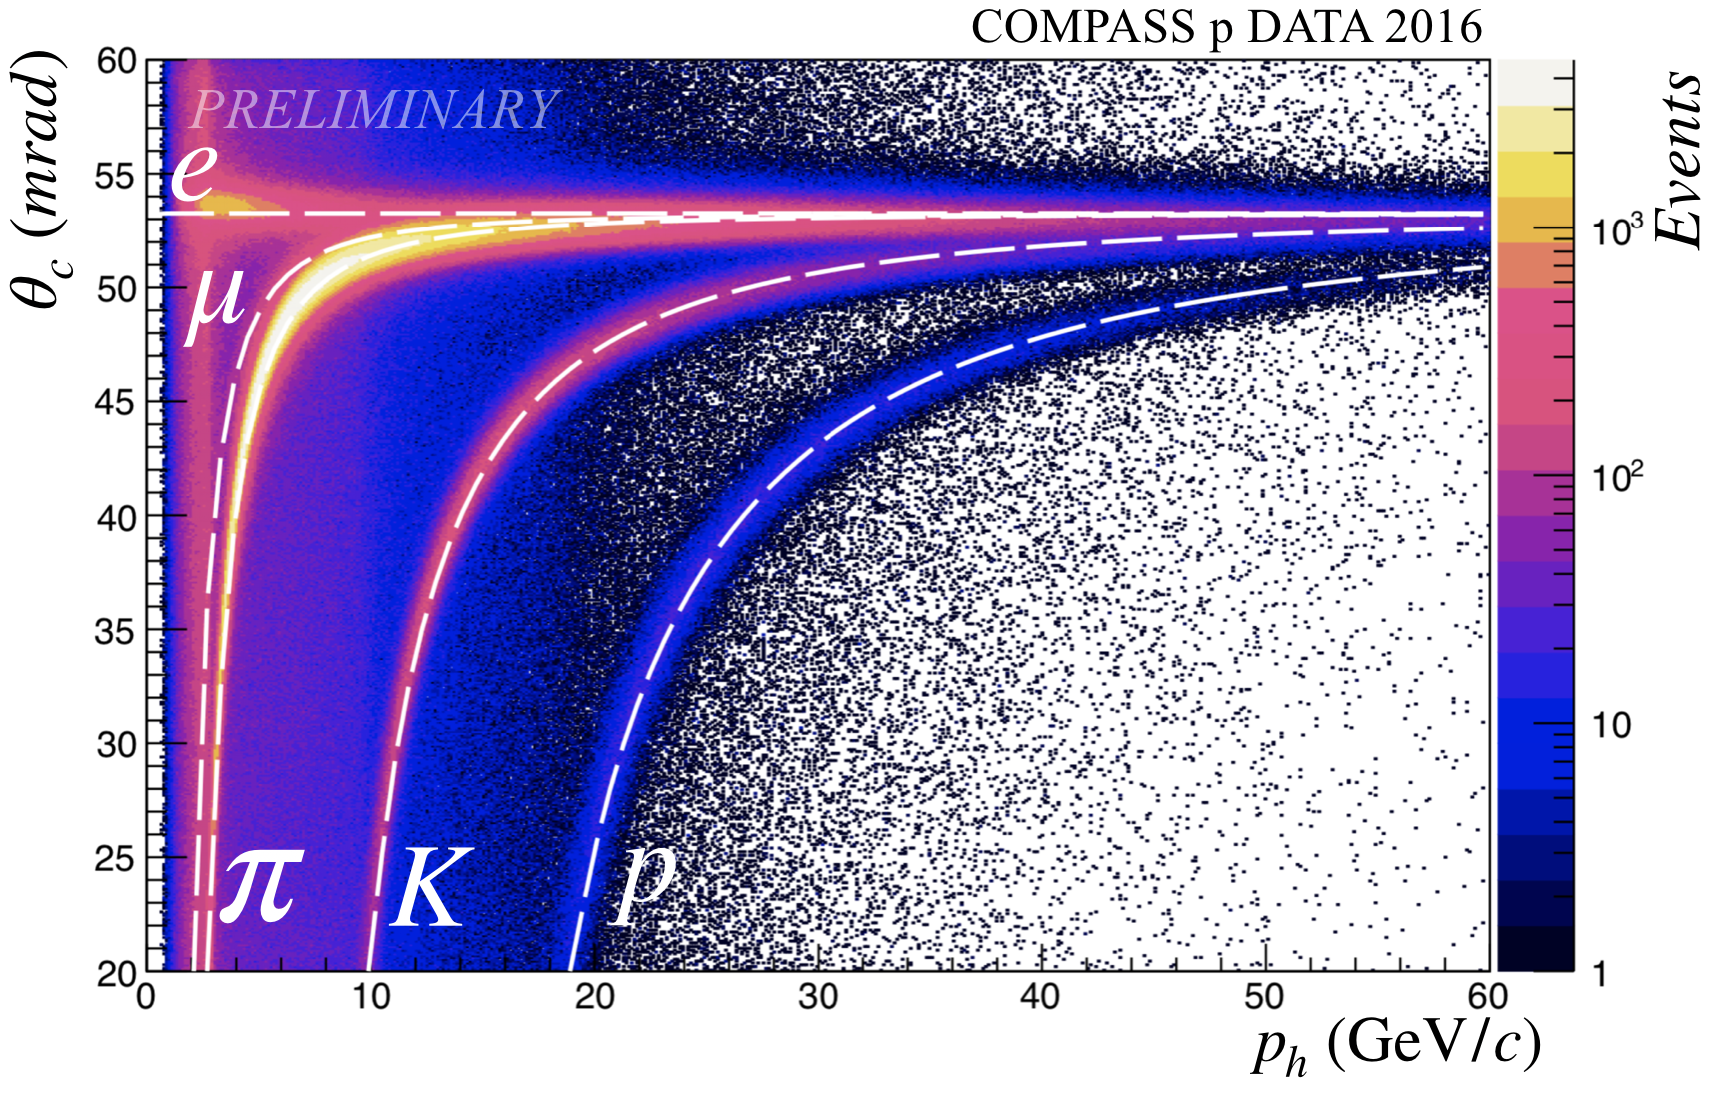
\includegraphics[scale=0.45]{./gfx/RICHIndices.png}
	\caption{Comparison of reconstructed Cherenkov angle as a function of the momentum with the calculated Cherenkov angle for each particle type using the refractive index of the RICH gas. This plot is not used for the PID.}
	\label{pic:RefIndex}
\end{figure}

\section{Method of unfolding}

The particle identification efficiency of the RICH is studied as a function of the hadron phase space. Here we use the hadron momentum and the polar angle at the entrance of the RICH, as already studied before, for example in Reference \cite{Curiel}. A fine binning is used for the momentum dependence, since the Cherenkov effect depends strongly on this variable. For the dependence on the polar angle, a coarse binning can be used, since only a weak dependence is observed. The binning used is:

\begin{itemize}
  \item Momentum $p_h$ (GeV/$c$): \{$3,5,7,10,12,13,15,17,19,22,25,27,30,35,40,50$\}
  \item Angle $\theta_h$ (rad): \{$0,0.01,0.04,0.12,0.3$\}
\end{itemize}

For each bin, the elements of the efficiency matrix $M_R$ are determined separately for positive and negative particles. The elements of this matrix contain the probability for a particle $t$ to be identified as a particle of type $i$, for example a pion that is correctly identified as pion or wrongly as a kaon. In the case of positive pions, the events from the $K^0$ sample are used, where the negative hadron is identified as a pion using the likelihood cuts shown in Table~\ref{tab:LHcut}.  Therefore, the second particle has to be a pion too, if the decaying particle was a $K^0$. Using the RICH, the particle type is determined for the second particle, which  results in the number $N(\pi^+ \rightarrow i)$. An equivalent procedure is used for positive kaons and protons using the $\Phi$ and $\Lambda$ samples. In order to obtain these numbers for the negative particles, the same samples are used but this time performing the identification of the positive particle in the first place. The numbers $N(t \rightarrow i)$ are extracted using a fit, which is described here for the $K^0$ sample, where the negative pion is already identified. The events are put into five different groups, depending on the particle type determined by the RICH:

\begin{itemize}
  \item All events (RICH not used for second particle)
  \item Events where $\pi^+$ is identified as $\pi^+$
  \item Events where $\pi^+$ is identified as $K^+$
  \item Events where $\pi^+$ is identified as $p$
  \item Events where $\pi^+$ is not identified
\end{itemize}

For each of these groups, the invariant $K^0$ mass spectra are shown in Fig.~\ref{pic:K0MassSpectra}, for a selected momentum bin. The number of events in the peak and the background are determined by a simultaneous fit of all five spectra. These spectra are described using two Gaussian distributions with the same mean for the signal, $f_{sig}$, and a polynomial to describe the background, $f_{bg}$. Their expressions are given in Table~\ref{tab:FunctionForm}. The two Gaussian distributions account for the different resolutions of the two spectrometer stages. The fitted function for each of the groups is given by
%
\begin{equation}
  f(x) = N_{sig} \cdot f_{sig} + N_{bg} \cdot f_{bg},
\end{equation}
%
where $N_{sig}$ is the amount of $K^0$ and $N_{bgd}$ the amount of background events. Here, the same widths, $\sigma_1$ and $\sigma_2$, of the two Gaussian distributions was used for all five spectra.

\begin{table}[!h]
  \caption{Functional form for the descriptin of the mass spectra for $K^0$, $\Phi$ and $\Lambda$ candidates from the clean samples. The symbol $G$ represents a Gaussian distribution and the symbol $BW$ a relative Breit-Wigner distribution.}
  \label{tab:FunctionForm}
  \centering
  \begin{tabular}{lcc}
    \hline
    SAMPLE & SIGNAL & BACKGROUND \\
    \hline
    $K^0$ & $\delta G(\mu,\sigma_1) + (1-\delta)G(\mu,\sigma_2)$ & $1+ax+b(2x^2-1)+c(4x^3-3x)$ \\
    $\Phi$ & $BW(\mu,\sigma_1) \otimes G(\mu,\sigma_2)$ & $(x-t)^n \cdot exp(-a(x-t))$ with $t=2 \cdot m_K$ \\
    $\Lambda$ & $\delta G(\mu,\sigma_1) + (1-\delta)G(\mu,\sigma_2)$ & $(x-t)^n \cdot exp(-a(x-t))$ with $t= m_p + m_{\pi}$ \\
    \hline
  \end{tabular}
\end{table}

\begin{figure}[!h]
  \centering
	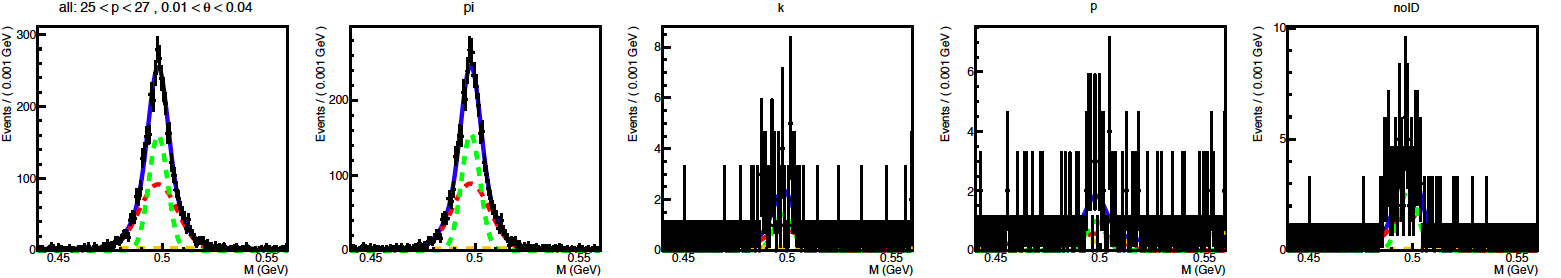
\includegraphics[scale=0.3]{./gfx/K0MassSpectra.png}
	\caption{Mass spectra for $K^0$ candidates with an identified $\pi^-$ for various hypotheses for the second hadron (from left to right: all, $\pi$, $K$, $p$, no ID). The momentum of the positive hadron is in the range of [$25$,$27$] GeV/$c$ and in the angle in the range [$0.01$,$0.04$] rad.}
	\label{pic:K0MassSpectra}
\end{figure}

Also the ratio $\delta$ of the amount of events in both Gaussian distributions is assumed to be the same. The shape of the background is the same for all spectra, except for the one where the pion is identified as a proton. In this case, a possible background contribution due to decays from $\Lambda$ baryons into a pion and an proton can be found. This results in a slightly different background shape. The integral of the background remains as an independent parameter in all five cases. In order to ensure that the sum of all efficiencies  ($\varepsilon(\pi^+ \rightarrow \pi^+)  + \varepsilon(\pi^+ \rightarrow K^+ ) + \varepsilon(\pi^+ \rightarrow p ) + \varepsilon(\pi^+ \rightarrow noID)$) is $100$\%, an additional constraint is introduced to the fit.
%
\begin{equation}
  N^{all}(K^0) = N^{\pi}(K^0) + N^{K}(K^0) + N^{p}(K^0) + N^{noID}(K^0),
\end{equation}
%
where $N_i(K^0)$ (i = $\pi$, $K$, $p$, $noID$) is the number of $K^0$ obtained from the histogram where the pion is identified as $i$. This results in $16$ free parameters of the fit.

The main difference between the fits of $K^0$, $\Phi$ and $\Lambda$ samples is the description of the signal and the background, while the same method is used. The functions describing both are also given in Table~\ref{tab:FunctionForm}. Again the parameters describing the shape are the same in all five spectra and the fit parameters  describing the integrals of the functions are used as free parameters, except for the parameter of the mass spectrum including all events. This results in $15$ free parameters for the fit of the $\Phi$ sample and in $15$ free parameters for the fit of the $\Lambda$ sample. Examples of the fits performed for the $\Phi$ and $\Lambda$ samples are shown in Figs.~\ref{pic:PhiMassSpectra} and \ref{pic:LambdaMassSpectra}. The figures show the results for the same momentum bin ($25$ GeV/$c$ $<$ $p_h$ $<$ $27$ GeV/$c$) and angular bin ($0.01$ rad $< \theta <$ $0.04$ rad), which was also shown for the $K^0$ sample.

\begin{figure}[!h]
  \centering
	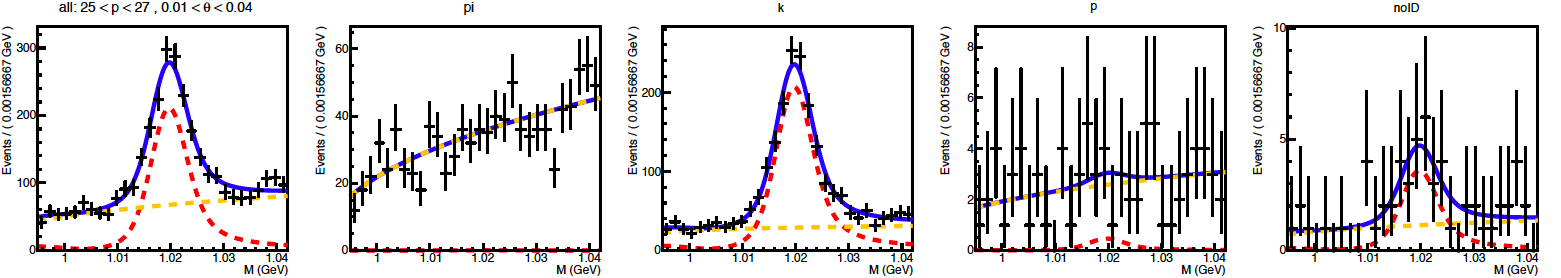
\includegraphics[scale=0.3]{./gfx/PhiMassSpectra.png}
	\caption{Mass spectra for $\Phi$ candidates with an identified $K^-$ for various hypotheses for the second hadron (from left to right: all, $\pi$, $K$, $p$, no ID). The momentum of the positive hadron is in the range of [$25$,$27$] GeV/$c^2$ and in the angle in the range [$0.01$,$0.04$] rad.}
	\label{pic:PhiMassSpectra}
\end{figure}

\begin{figure}[!h]
  \centering
	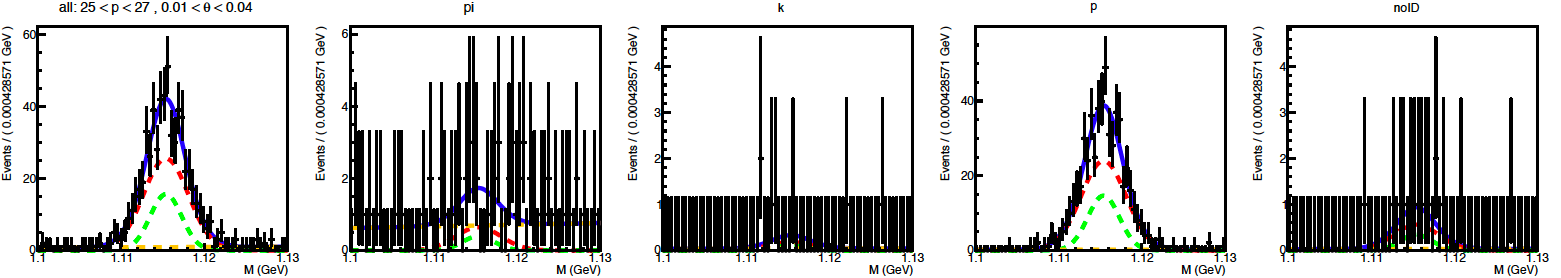
\includegraphics[scale=0.3]{./gfx/LambdaMassSpectra.png}
	\caption{Mass spectra for $\Lambda$ candidates with an identified $\pi^-$ for various hypotheses for the second hadron (from left to right: all, $\pi$, $K$, $p$, no ID). The momentum of the positive hadron is in the range of [$25$,$27$] GeV/$c^2$ and in the angle in the range [$0.01$,$0.04$] rad.}
	\label{pic:LambdaMassSpectra}
\end{figure}

\section{Calculation of the efficiencies and uncertainties}

The elements of the efficiency matrix $M_R$ are determined from fitted numbers of signal events,

\begin{equation}
  \epsilon(t\rightarrow i) = \frac{N(t\rightarrow i)}{N(t)}
\end{equation}

Here, $N(t)$ is given by the sum of all $N(t \rightarrow i)$. As the nominator and denominator are correlated, the uncertainty has to be determined via error propagation taking into account the covariance matrix of the fit,

\begin{equation}
  \Delta \epsilon = \sqrt{\sum_{j=1}^m \left( \frac{\delta \epsilon}{\delta N(i\rightarrow j)} \right)^2 \cdot u_j + 2 \sum_{j=1}^{m-1} \sum_{k=j+1}^{m} \left( \frac{\delta \epsilon}{\delta N(i\rightarrow j)} \frac{\delta \epsilon}{\delta N(i\rightarrow k)} \cdot u(j,k) \right)}
\end{equation}

where $u_j$ are the diagonal elements of the covariance matrix, $u(i,j)$ are the off diagonal elements and $\epsilon$ is one of the elements of the efficiency matrix. The summations are done over all possible particle types i.e. pion, kaon, proton and non identified.

\section{Results} \label{sec:Results}

The results for the RICH particle identification efficiency are shown in Figs. \ref{pic:Effpip} to \ref{pic:Effkp} for $\pi^+$ and $K^+$ for the various particle types and charges. The plots for the other species can be found in Appendix~\ref{app:RICH}. In each figure, the momentum dependence for the different angular bins is shown. The efficiencies are weakly dependent on the angle, while it is more strongly correlated with the momentum, especially in the region near the threshold.

\begin{figure}[!p]
  \centering
	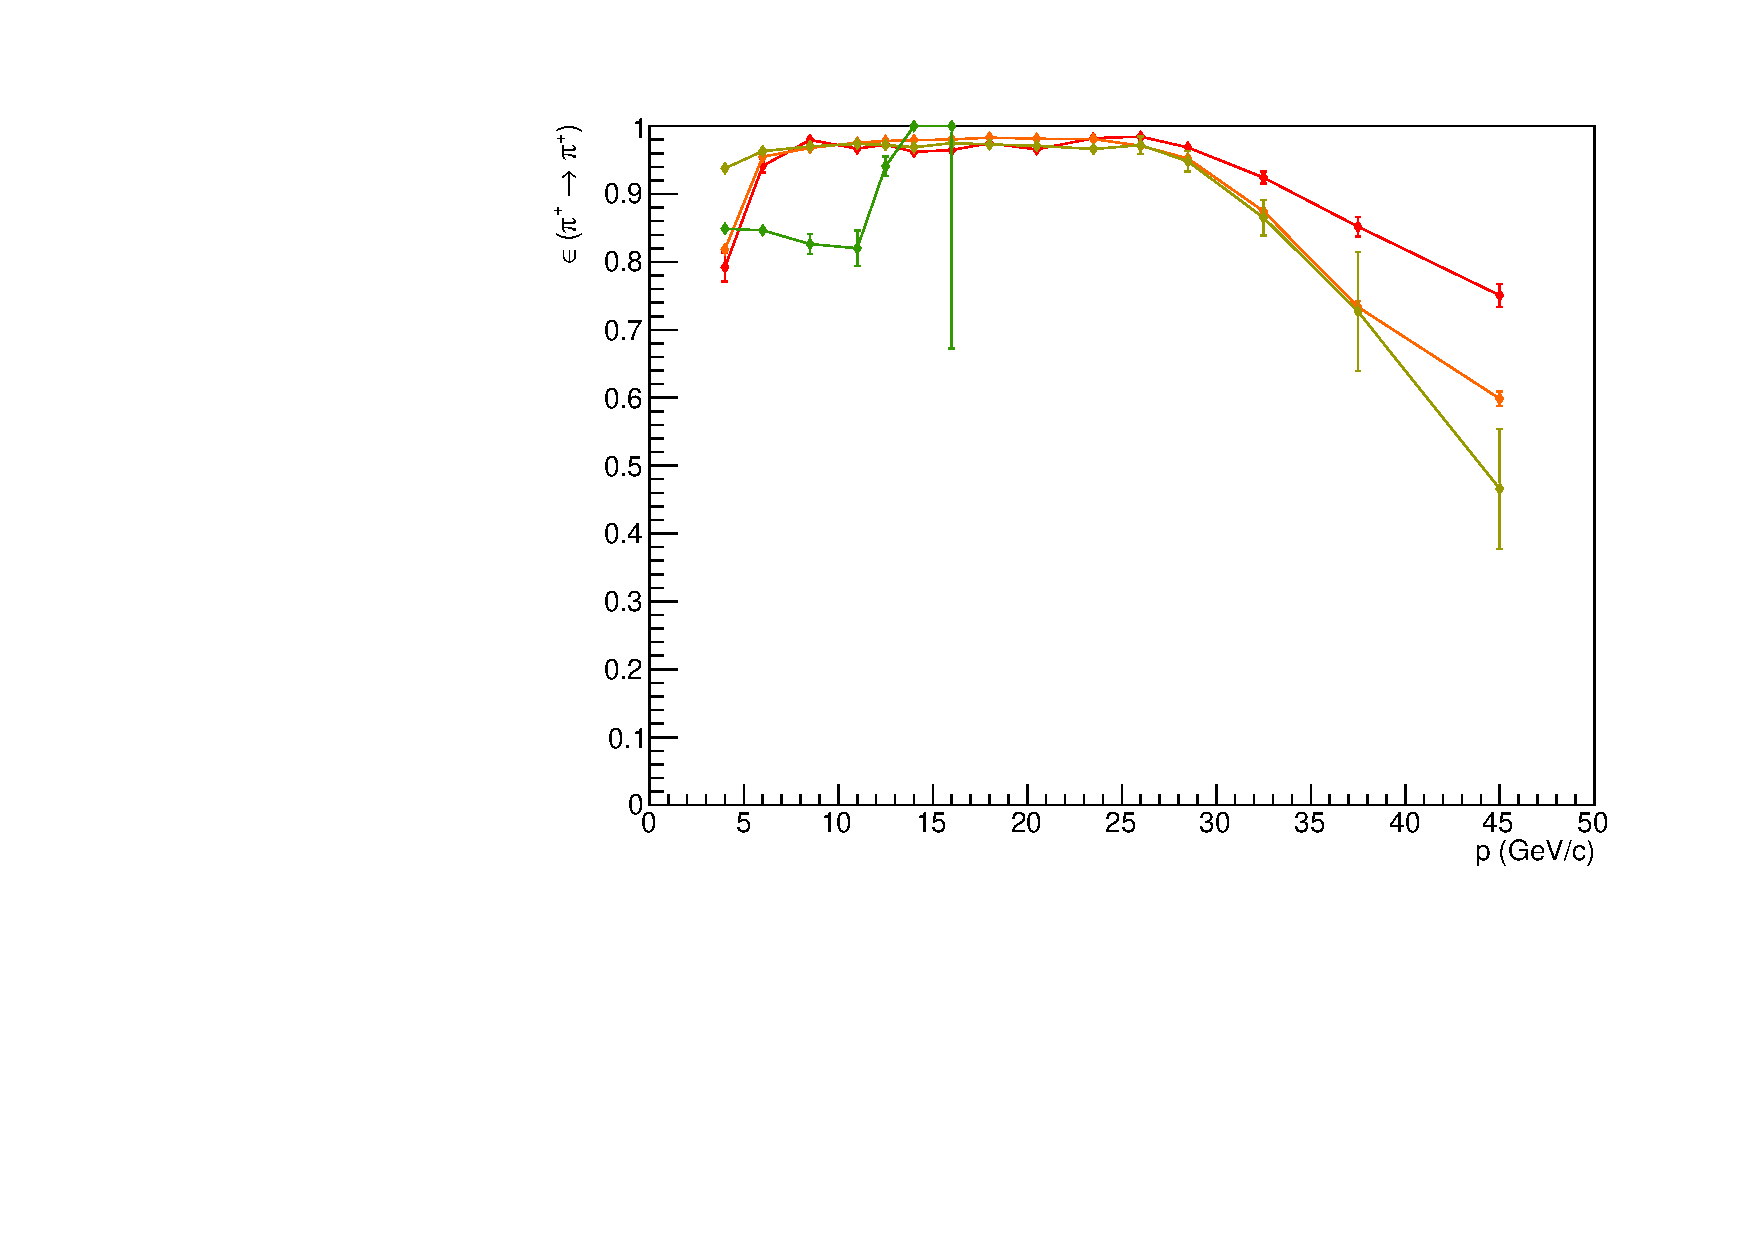
\includegraphics[scale=0.35]{./gfx/pip_pi.pdf}
  \includegraphics[scale=0.35]{./gfx/pip_K.pdf}
  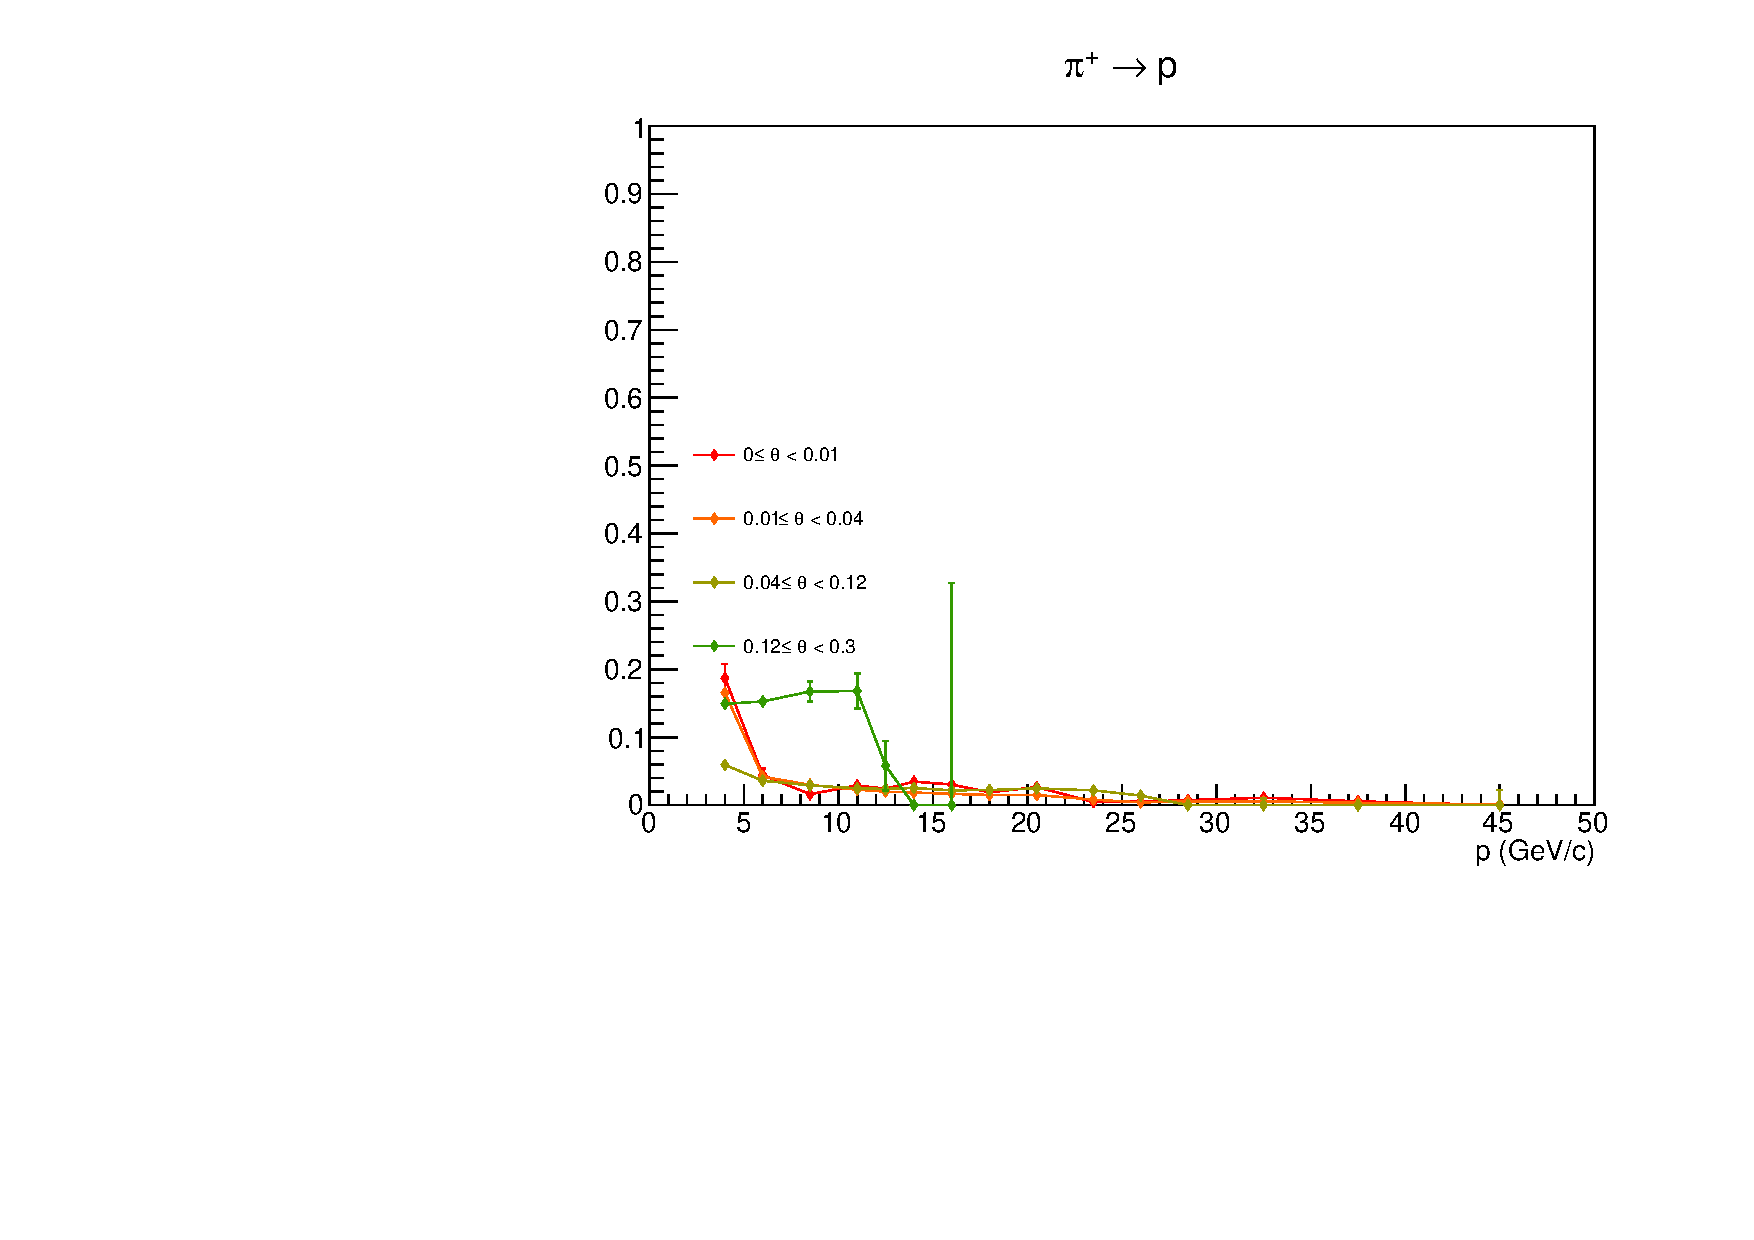
\includegraphics[scale=0.35]{./gfx/pip_p.pdf}
  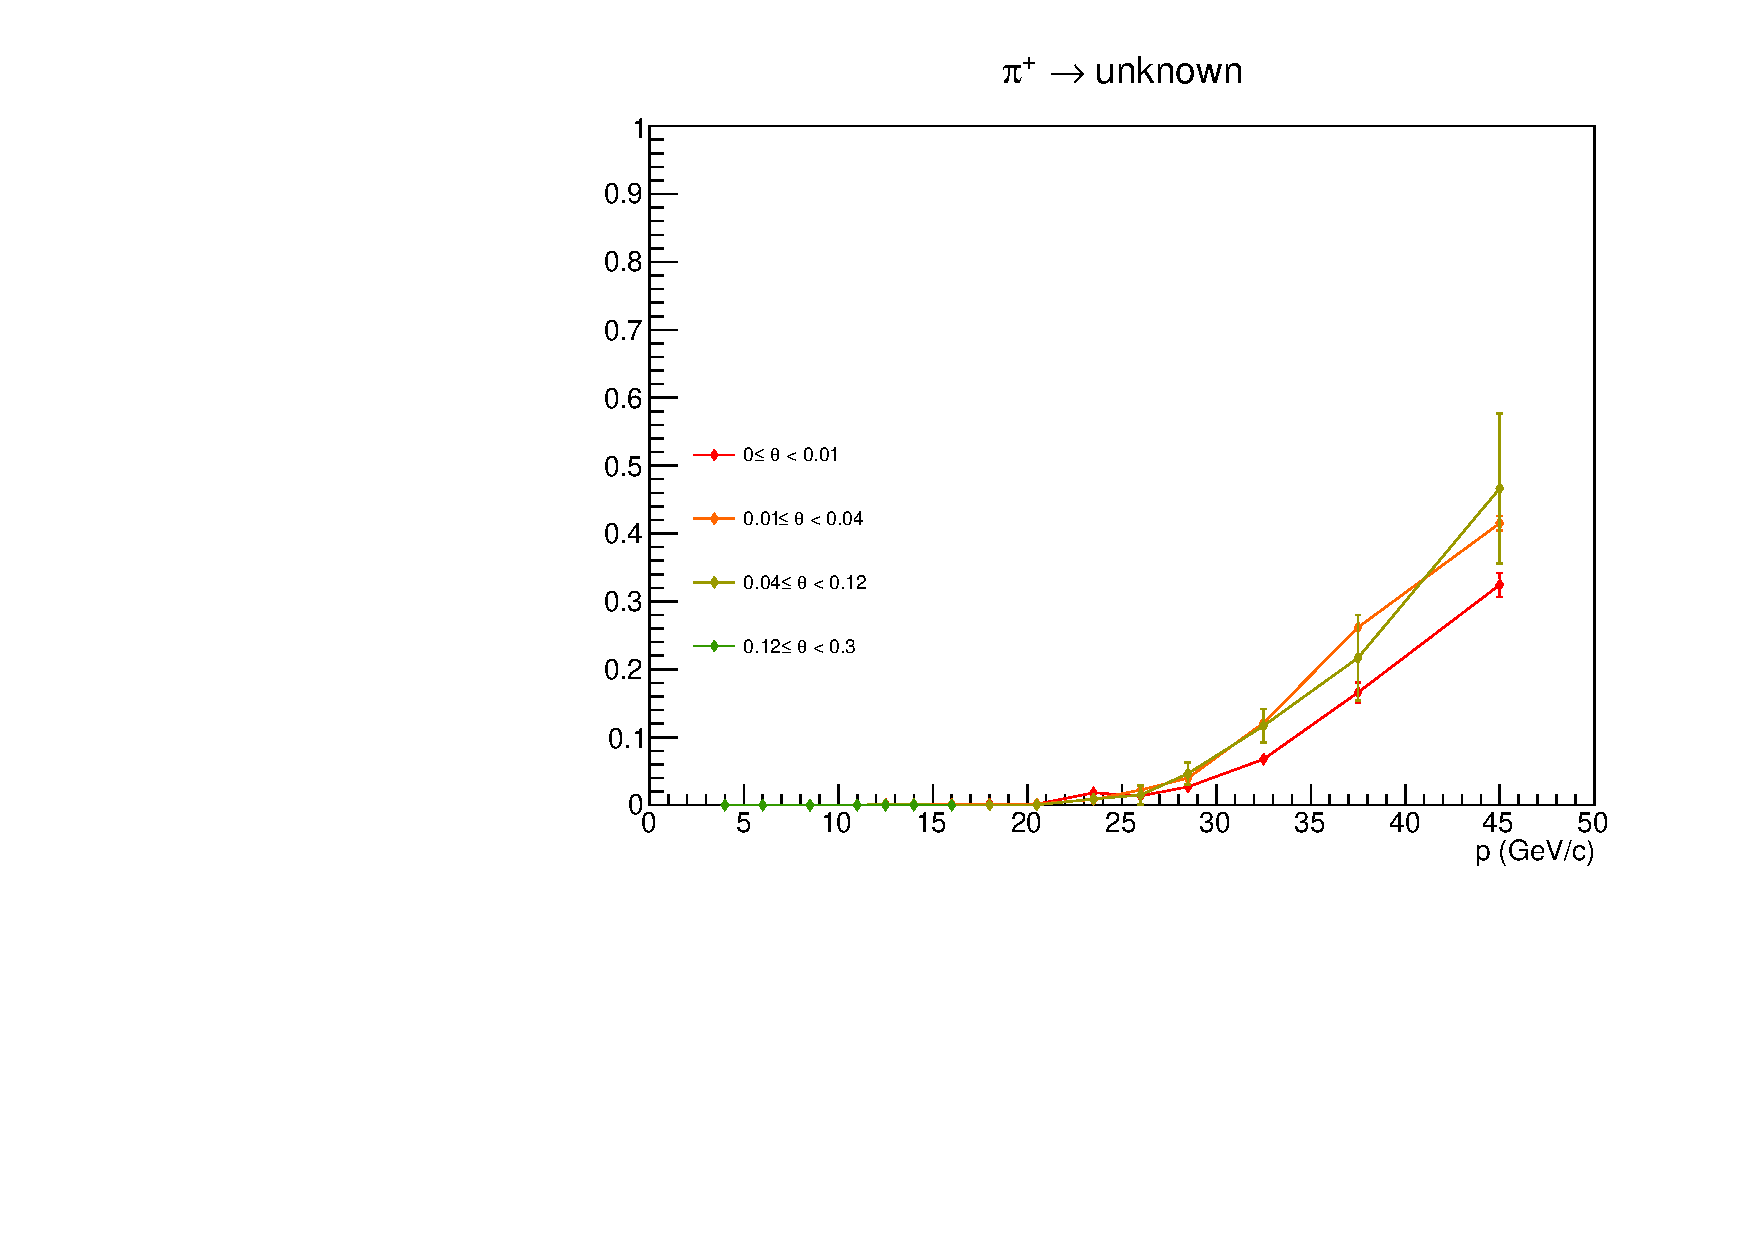
\includegraphics[scale=0.35]{./gfx/pip_u.pdf}
	\caption{Identification probabilities $\epsilon(p \rightarrow j)$ for $\pi^+$.}
	\label{pic:Effpip}
\end{figure}

\begin{figure}[!p]
  \centering
	\includegraphics[scale=0.35]{./gfx/Kp_pi.pdf}
  \includegraphics[scale=0.35]{./gfx/Kp_K.pdf}
  \includegraphics[scale=0.35]{./gfx/Kp_p.pdf}
  \includegraphics[scale=0.35]{./gfx/Kp_u.pdf}
	\caption{Identification probabilities $\epsilon(p \rightarrow j)$ for $K^+$.}
	\label{pic:Effkp}
\end{figure}

The RICH performs a correct identification of pions in more than $95$\% of the cases for momenta below 30 GeV/$c^2$ and the probability for a misidentification of a pion as a kaon is below $\sim$ $1$\%. For kaons, near the threshold, a strong momentum dependence of the efficiencies is observed. Therefore a cut of $12$ GeV is chosen in the following analysis. At higher momenta the correct identification is given in $\sim$ $95$\% of the cases and the probability for a misidentification of a kaon as a pion is below $\sim$ $2$\%. For protons, the momentum dependence around threshold level is even stronger. Below the threshold, protons are identified correctly in $50$\% of the cases. Above the threshold numbers rise to $\sim$ $95$\%.

\section{Problem at high $z$}

At some point it was discovered that at high momenta and high $z$ ($35$ GeV/$c$ < $p_h$ < $40$ GeV/$c$, $z$ > $0.7$), a contamination of the kaon sample by misidentified pions was observed, which was not accounted for in the efficiency matrix (Fig.~\ref{pic:NonLin}). Instead of the expected separation between pions and kaons at $LH_{\pi} = LH_K$, pions are found at $LH_{\pi} < LH_K$. We are now not looking at the clean samples but back to the normal data.

\begin{figure}[!h]
  \centering
	\includegraphics[scale=0.35]{./gfx/RICHLH.png}
	\caption{Likelihood for pions as a function of the likelihood for kaons using 2016 data.}
	\label{pic:NonLin}
\end{figure}

The larger the likelihood values are, the larger the effect is. This behaviour is also present in $2006$, $2007$ and $2011$ data (Fig. \ref{pic:NonLinother}). When investigating, it was shown that the probability for the misidentification of pions as kaons differs from the value given in the RICH tables in this kinematic region using the $p_T$ spectra \cite{MarcinNote}.

\begin{figure}[!h]
  \centering
	\includegraphics[scale=0.2]{./gfx/RICHLH2006.png}
  \includegraphics[scale=0.3]{./gfx/RICHLH2011.png}
	\caption{Likelihood for pions as a function of the likelihood for kaons using (from left to right) $2006$, $2007$ and $2011$ data.}
	\label{pic:NonLinother}
\end{figure}

In order to check if the non-linearities are taken correctly into account in the RICH tables, the likelihood values for pions and kaons are compared using the $K^0$ sample for high momenta and high $z$. This comparison is shown in Fig. \ref{pic:K0sample}, highlighting the fact that the problematic region is not covered by the $K^0$ sample and therefore the RICH table are not valid in this kinematic region.

\begin{figure}[!h]
  \centering
	\includegraphics[scale=0.4]{./gfx/K0sample.png}
	\caption{Likelihood for pions as a function of the likelihood for kaons using the 2011 $K^0$ sample. Figure taken from \cite{RICHnote}.}
	\label{pic:K0sample}
\end{figure}

In order to obtain correct values for the RICH tables, a different sample for pions is needed. This new sample is obtained using the $\rho^0$ decay into two pions. The sample contains, in contrast to the $K^0$ sample, events at high momenta and high $z$, which covers high likelihood values. Though this method has been working for the $2006$ data it was not concluding with $2016$ data probably due to the lower statistics available for the current analysis compared to what was used in $2006$.

\begin{figure}[!h]
  \centering
	\subfloat[]{\includegraphics[scale=0.28]{./gfx/NewRICH1.png}}
  \subfloat[]{\includegraphics[scale=0.3]{./gfx/NewRICH2.png}}
	\caption{Figure (a) displays the likelihood ratio $L_{K}/L_{\pi}$ before (blue curve) and after (red curve) the new alignement of the RICH. The separation minimum is visible at $L_{K}/L_{\pi} = 1$ with the new alignement. Figure (b) compares the likelihood ratio $L_{K}/L_{\pi}$ for $z>0.6$ (magenta curve) and $z<0.4$ (green curve). While previously likelihoods were perfoming worse with $z$, the trend is as expected with the new alignement. Figures taken from \cite{MarcinNew}.}
	\label{pic:newRICH}
\end{figure}

These non-linearities have been adressed recently by the COMPASS RICH group. They have been reporting that the mirrors were not placed at the right place. A refinement of the alignement has an effect on the refractive index extraction and subsequently improving the pion versus kaon likelihoods picture, apparently curing the non-linearities. Further tests must still be done in order to quantify the improvement but preliminary studies \cite{MarcinNew} displayed in Fig.~\ref{pic:newRICH} show for the moment that the misidentification problem adressed in this section has been corrected. The $\pi$ peak is now below $L_{K}/L_{\pi} = 1$ and the separation minimum close to $L_{K}/L_{\pi} = 1$ is visible. In addition, while previously likelihoods were performing worse at high $z$, now the trend is as expected. This new alignement of the RICH has not been taken into account in the following analysis.

\section{Comparison of the efficiencies of 2006 to 2016}

In order to see if the RICH has been stable in terms of efficiency and purity through time, it is possible to compare the RICH efficiencies for $2006$, $2011$ and $2016$ (Fig. \ref{pic:comppip} to \ref{pic:comppm}). The first data taking with the refurbished RICH was done in $2006$. All these effiencies are extracted using the same likelihood cuts. The results point to a good stability of the RICH through time, even improving for some efficiencies, like pion identification for example. All data support the good identification of all species in the selected momentum range highlighting the excellent separation performed by the RICH.

\begin{figure}[!h]
  \centering
	\includegraphics[scale=0.35]{./gfx/t1/pip2pip.png}
  \includegraphics[scale=0.35]{./gfx/t1/pip2kp.png}
  \includegraphics[scale=0.35]{./gfx/t1/pip2pp.png}
	\caption{Identification probabilities $\epsilon(p \rightarrow j)$ for $\pi^+$ in the bin $0.01$ rad $<$ $\theta_h$ $<$ $0.04$ rad for 3 different years: 2006 (blue), 2011 (orange) and 2016 (green).}
	\label{pic:comppip}
\end{figure}

\begin{figure}[!p]
  \centering
	\includegraphics[scale=0.35]{./gfx/t1/pim2pim.png}
  \includegraphics[scale=0.35]{./gfx/t1/pim2km.png}
  \includegraphics[scale=0.35]{./gfx/t1/pim2pm.png}
	\caption{Same as Fig.~\ref{pic:comppip} for $\epsilon(p \rightarrow j)$.}
	\label{pic:comppim}
\end{figure}

\begin{figure}[!p]
  \centering
	\includegraphics[scale=0.35]{./gfx/t1/kp2pip.png}
  \includegraphics[scale=0.35]{./gfx/t1/kp2kp.png}
  \includegraphics[scale=0.35]{./gfx/t1/kp2pp.png}
	\caption{Same as Fig.~\ref{pic:comppip} for $\epsilon(p \rightarrow j)$.}
	\label{pic:compkp}
\end{figure}

\begin{figure}[!p]
  \centering
	\includegraphics[scale=0.35]{./gfx/t1/km2pim.png}
  \includegraphics[scale=0.35]{./gfx/t1/km2km.png}
  \includegraphics[scale=0.35]{./gfx/t1/km2pm.png}
	\caption{Same as Fig.~\ref{pic:comppip} for $\epsilon(p \rightarrow j)$.}
	\label{pic:compkm}
\end{figure}

\begin{figure}[!p]
  \centering
	\includegraphics[scale=0.35]{./gfx/t1/pp2pip.png}
  \includegraphics[scale=0.35]{./gfx/t1/pp2kp.png}
  \includegraphics[scale=0.35]{./gfx/t1/pp2pp.png}
	\caption{Same as Fig.~\ref{pic:comppip} for $\epsilon(p \rightarrow j)$.}
	\label{pic:comppp}
\end{figure}

\begin{figure}[!h]
  \centering
	\includegraphics[scale=0.35]{./gfx/t1/pm2pm.png}
  \includegraphics[scale=0.35]{./gfx/t1/pm2km.png}
  \includegraphics[scale=0.35]{./gfx/t1/pm2pm.png}
	\caption{Same as Fig.~\ref{pic:comppip} for $\epsilon(p \rightarrow j)$ for $\bar{p}$.}
	\label{pic:comppm}
\end{figure}

%----------------------------------------------------------------------------------------

\newpage

\section{Summary}

The RICH detector performances are determined from real data, using samples of $\pi$, $K$ and $p$ coming from the decay into two charged particles of $K^0$, $\Phi$ and $\Lambda$. In order to take into account the dependence of the RICH performance with the hadron phase-space, the performances are extracted in bins of the particle momentum $p_h$ and the track polar angle $\theta_h$ at the RICH entrance.

High identification probabilities are reached for $p_h$ below $30$ GeV/$c$. For pions, it reaches values larger than $97\%$ and for kaons and protons, it reaches values larger than $90\%$ except for the zones around the kaon and proton thresholds of $\sim$ $9.45$ and $\sim$ $17.95$ GeV/$c$, respectively. The identification probability values drop for larger $p_h$ values in the pion and kaon case due to the Cherenkov angle saturation ($\beta \rightarrow 1$). As a consequence, the misidentification probabilities are larger in this region.
 % RICH PID

\cleardoublepage % Empty page before the start of the next part

%------------------------------------------------

\part{DJANGOH : a Monte-Carlo generator with Radiative Corrections} % Third part of the thesis

% Chapter 6

\chapter{DJANGOH} % Chapter title

\label{ch:DJANGOH} % For referencing the chapter elsewhere, use \autoref{ch:name}

%----------------------------------------------------------------------------------------

\section{Features of DJANGOH}

Content

%------------------------------------------------

\subsection{Subsection Title}

Content

%------------------------------------------------

\subsection{Subsection Title}

Content

%----------------------------------------------------------------------------------------

\section{Enhancement of DJANGOH}

Content

%----------------------------------------------------------------------------------------

\section{TDJANGOH Interface}

Content
 % TERAD, RADGEN, DJANGOH
% Chapter 7

\chapter{Results on Radiative Corrections} % Chapter title

\label{ch:RC} % For referencing the chapter elsewhere, use \autoref{ch:name}

%----------------------------------------------------------------------------------------

\section{Inclusive and Semi-Inclusive Radiative Correction factors}

The calculation of the inclusive radiative correction factors can be done by computing
$\sigma_{Born}$ and $\sigma_{Born+o(\alpha)}$. A correct way to obtain these factors is the following :

\[\eta(x,y)=\frac{\sigma_{Born}(x,y)}{\sigma_{Born+o(\alpha)}(x,y)}
=\frac{\frac{\sigma_{Born,tot}*N_{Born}(x,y)}{N_{Born,tot}}}{\frac{\sigma_{Born+o(\alpha),tot}*N_{Born+o(\alpha)}(x,y)}{N_{Born+o(\alpha),tot}}}\]

The results that are presented below are obtained with the TERAD $F_{2}$ and R parametrizations, which
describes accurately the behaviour of $F_{2}$ at low $Q^{2}$\cite{BPnote} :

\begin{itemize}
\item $F^{p}_{2}(x,Q2)$ for $Q^2 > 0.2$ GeV$^2$ and $0.000035 < x < 0.85$, as obtained from a fit to the
world proton (and deuteron) data made by the SMC\cite{SMC}.
\item For $Q^2 < 0.2$ GeV$^2$, a phenomenological model of Badelek and Kwiecinski\cite{BK}, valid at $10^{-5} < x < 0.1$
and $0 < Q^2 < 1000$ GeV$^2$.
\item $R(x, Q^2)$ as parameterised by SLAC (newer version, called R1998\cite{R1998}), valid for $Q^2 > 0.5$ GeV$^2$, extended
to lower values of Q2, including the $R \simeq Q^2$ behaviour at $Q^2 = 0$.
\end{itemize}

The $o(\alpha)$ are included except for quark line radiation. The reason why these corrections are not
included is that these corrections are negligible except at large $x \geq 0.5$ and $Q^{2} \geq 10^3$ GeV$^2$,
where the corrections reach the magnitude of barely one percent (see Fig. \ref{fig:quarkline}). Also, even though this is not the
case in TERAD $F_{2}$, these corrections are often not subtracted inside the parametrization, thus
they are already taken into account in the parametrization\cite{HubertF2Rad}.

\begin{figure}[htb]
\centerline{\epsfig{file=gfx/quarkline.png,width=12cm}}
\caption{$Q^2$ dependence of the quarkonic QED corrections (in percent) to the structure function $F^2_p$ for deep inelastic
lepton-proton scattering at $x=0.001$, $x=0.1$ and $x=0.505$.}\label{fig:quarkline}
\end{figure}

The kinematic range for the presented results is $x \in [0.004,0.9]$ and $y \in [0.1,0.9]$.

Overall, the corrections on the considered kinematic space are within 10\% except for high $y$ corrections
that go up to 40\%.

\newpage

\subsection{Semi-Inclusive radiative correction factors : Effect on Multiplicities}

The calculation of the semi-inclusive radiative correction factors can be done by computing
$M^{h^{\pm}}_{Born}$, multiplicities obtained without radiative corrections, and $M^{h^{\pm}}_{Born+o(\alpha)}$,
multiplicities obtained with radiative corrections. A correct way to obtain these factors is the following :

\[\eta^{h^{\pm}}(x,y,z)=\frac{M^{h^{\pm}}_{Born}(x,y,z)}{M^{h^{\pm}}_{Born+o(\alpha)}(x,y,z)}\]

In the following plots, the cuts from the SIDIS analysis for the selection of DIS events and
hadrons are used. For more information, please refer to the multiplicities papers\cite{Mult}. I will explicitate
the kinematical cuts that are used :

\begin{itemize}
\item $0.004 \leq x_{Bj} \leq 0.4, x_{Bj} \in \{.004,.01,.02,.03,.04,.06,.1,.14,.18,.4\}$
\item $0.1 \leq y \leq 0.7, y \in \{.1,.15,.2,.3,.5,.\}$
\item $3 \leq p_h \leq 40$ GeV
\end{itemize}

Fig. \ref{fig:hadz_ratio} exhibits the semi-inclusive radiative correction factor $\eta^{h^{\pm}}(x,y,z)$. This factor goes from 0\% correction
at low $z$ and low $y$ to 10\% correction at high $z$ and high $y$. This dependance on $y$ and $z$ is expected (eg. if a hadron has a high
$z$ in a non-radiative event, consider the same event but with the radiation of a real photon, $\nu_{lep}$ will remain the same but the hadron will have
in reality less energy available from the virtual photon, thus having $z_{had} \leq z_{lep}$, leading to less events in the high $z$ region for the multiplicities
obtained with radiative corrections).

Another view on the semi-inclusive correction is given by Fig. \ref{fig:hadpt_ratio}, where the $z$ binning is replaced with a
$p_T$ ($\eta^{h^{\pm}}(x,y,p_T)$). The factor goes from -20\% correction at high $p_T$, high $y$ and high $x$
to +10\% correction at low $y$, high $x$ and high $p_T$.

When looking at $\eta^{\pi^{\pm}}(x,y,z)$ and $\eta^{K^{\pm}}(x,y,z)$, the corrections are very similar to $\eta^{h^{\pm}}(x,y,z)$.

\newpage
\begin{figure}[!htb]
\centerline{\epsfig{file=gfx/hadron_ratio.pdf,width=18cm}}
\caption{$\eta^{h^{\pm}}(x,y,z)$, positive hadrons in full points, negative in voided points, in bins of $x$, staggered with $y$ and versus $z$.
The corrections go from 0\% at low $z$ and low $y$ to 10\% at high $z$ and high $y$}\label{fig:hadz_ratio}
\end{figure}

\begin{figure}[!htb]
\centerline{\epsfig{file=gfx/hadron_pt_ratio.pdf,width=18cm}}
\caption{$\eta^{h^{\pm}}(x,y,p_T)$, positive hadrons in full points, negative in open points, in bins of $x$, staggered with $y$ and versus $p_T$.
The corrections go from -20\% at high $p_T$, high $y$ and high $x$ to +10\% at low $y$, high $x$ and high $p_T$.}\label{fig:hadpt_ratio}
\end{figure}

\newpage

\begin{figure}[!htb]
\centerline{\epsfig{file=gfx/pion_ratio.pdf,width=18cm}}
\caption{$\eta^{\pi^{\pm}}(x,y,z)$, positive hadrons in full points, negative in open points, in bins of $x$, staggered with $y$ and versus $z$.
Same conclusions as in Fig. \ref{fig:hadz_ratio} can be made.}\label{fig:piz_ratio}
\end{figure}

\begin{figure}[!htb]
\centerline{\epsfig{file=gfx/kaon_ratio.pdf,width=18cm}}
\caption{$\eta^{K^{\pm}}(x,y,z)$, positive hadrons in full points, negative in open points, in bins of $x$, staggered with $y$ and versus $z$.
Same conclusions as in Fig. \ref{fig:hadz_ratio} can be made.}\label{fig:kz_ratio}
\end{figure}

%----------------------------------------------------------------------------------------

\section{Comparison between DJANGOH and TERAD}

In the next figures, DJANGOH results are compared with TERAD\cite{TERAD}. The two programs are using the same set of
$F^{p}_{2}$ and $R$. This are the only inputs (apart from the process input ie. $\mu p$ scattering
at 160 GeV muon energy) that need to be identical so that the comparison is relevant.
One thing to be noted is that TERAD is using more complete sets of correction. They should have
an impact on the cross-section of TERAD, but are negligible.

The first check for consistency is to compare the $\sigma_{Born}$ of both programs.
Using the same input information on $F^{p}_{2}(x,Q2)$ and $R(x, Q^2)$ does not guarantee that $\sigma_{Born}$
for both program, called $\sigma^{D}_{Born}$ and $\sigma^{T}_{Born}$, is the same : the reason is that for example
in TERAD, $\sigma^{T}_{Born}$ is computed without constants like $\pi$, $M_{proton}$, $\alpha$, etc. and
its functional form is unknown, unlike in DJANGOH. This means that the ratio $r=\frac{\sigma^{D}_{Born}}{\sigma^{T}_{Born}}$
may differ from 1 but must be constant as a function of $x$ and $y$. Fig. \ref{fig:BRy} shows that this
is the case.

\begin{figure}[htb]
\centerline{\epsfig{file=gfx/BRy.pdf,width=12cm}}
\caption{Ratio of the Born cross-sections calculated with DJANGOH and TERAD, for the same input, as a function of y
at different values of x (staggered points at fixed y)}\label{fig:BRy}
\end{figure}

The radiative correction factors $\eta(x,y)$ for DJANGOH and TERAD are compared in Fig. \ref{fig:RCy}. The absolute
difference is then plotted in Fig. \ref{fig:ERy}, showing that the two programs differ at most 3\% in the region
of lowest x and highest y.


\begin{figure}[htb]
\centerline{\epsfig{file=gfx/RCy.pdf,width=12cm}}
\caption{Comparison of radiative corrections factor $\eta(y)$ for fixed values of x, computed for proton target at 160 GeV
and with the input information given above. Green dots mark results of TERAD, blue triangles the results of DJANGOH.}\label{fig:RCy}
\end{figure}

\begin{figure}[htb]
\centerline{\epsfig{file=gfx/ERy_scat.pdf,width=12cm}}
\caption{Ratio of radiative corrections factors obtained in Fig. \ref{fig:RCy}, $(\eta_T/\eta_D)-1$ as a function of y for fixed values of x}\label{fig:ERy}
\end{figure}
 % RADGEN issues
% Chapter 7

\chapter{Results on Radiative Corrections} % Chapter title

\label{ch:RC} % For referencing the chapter elsewhere, use \autoref{ch:name}

%----------------------------------------------------------------------------------------

\section{Inclusive and Semi-Inclusive Radiative Correction factors}\label{sec:RCF}

The calculation of the inclusive radiative correction factors can be done by computing
$\sigma_{Born}$ and $\sigma_{Born+o(\alpha)}$. A correct way to obtain these factors is the following :

\[\eta(x,y)=\frac{\sigma_{Born}(x,y)}{\sigma_{Born+o(\alpha)}(x,y)}
=\frac{\frac{\sigma_{Born,tot}*N_{Born}(x,y)}{N_{Born,tot}}}{\frac{\sigma_{Born+o(\alpha),tot}*N_{Born+o(\alpha)}(x,y)}{N_{Born+o(\alpha),tot}}}\]

The results that are presented below are obtained with the TERAD $F_{2}$ and R parametrizations, which
describes accurately the behaviour of $F_{2}$ at low $Q^{2}$\cite{BPnote} :

\begin{itemize}
\item $F^{p}_{2}(x,Q2)$ for $Q^2 > 0.2$ GeV$^2$ and $0.000035 < x < 0.85$, as obtained from a fit to the
world proton (and deuteron) data made by the SMC\cite{SMC}.
\item For $Q^2 < 0.2$ GeV$^2$, a phenomenological model of Badelek and Kwiecinski\cite{BK}, valid at $10^{-5} < x < 0.1$
and $0 < Q^2 < 1000$ GeV$^2$.
\item $R(x, Q^2)$ as parameterised by SLAC (newer version, called R1998\cite{R1998}), valid for $Q^2 > 0.5$ GeV$^2$, extended
to lower values of Q2, including the $R \simeq Q^2$ behaviour at $Q^2 = 0$.
\end{itemize}

The $o(\alpha)$ are included except for quark line radiation. The reason why these corrections are not
included is that these corrections are negligible except at large $x \geq 0.5$ and $Q^{2} \geq 10^3$ GeV$^2$,
where the corrections reach the magnitude of barely one percent (see Fig. \ref{fig:quarkline}). Also, even though this is not the
case in TERAD $F_{2}$, these corrections are often not subtracted inside the parametrization, thus
they are already taken into account in the parametrization\cite{HubertF2Rad}.

\begin{figure}[htb]
\centerline{\epsfig{file=gfx/quarkline.png,width=12cm}}
\caption{$Q^2$ dependence of the quarkonic QED corrections (in percent) to the structure function $F^2_p$ for deep inelastic
lepton-proton scattering at $x=0.001$, $x=0.1$ and $x=0.505$.}\label{fig:quarkline}
\end{figure}

The kinematic range for the presented results is $x \in [0.004,0.9]$ and $y \in [0.1,0.9]$.

Overall, the corrections on the considered kinematic space are within 10\% except for high $y$ corrections
that go up to 40\%.

\newpage

\subsection{Semi-Inclusive radiative correction factors : Effect on Multiplicities}

The calculation of the semi-inclusive radiative correction factors can be done by computing
$M^{h^{\pm}}_{Born}$, multiplicities obtained without radiative corrections, and $M^{h^{\pm}}_{Born+o(\alpha)}$,
multiplicities obtained with radiative corrections. A correct way to obtain these factors is the following :

\[\eta^{h^{\pm}}(x,y,z)=\frac{M^{h^{\pm}}_{Born}(x,y,z)}{M^{h^{\pm}}_{Born+o(\alpha)}(x,y,z)}\]

In the following plots, the cuts from the SIDIS analysis for the selection of DIS events and
hadrons are used. For more information, please refer to the multiplicities papers\cite{Mult}. I will explicitate
the kinematical cuts that are used :

\begin{itemize}
\item $0.004 \leq x_{Bj} \leq 0.4, x_{Bj} \in \{.004,.01,.02,.03,.04,.06,.1,.14,.18,.4\}$
\item $0.1 \leq y \leq 0.7, y \in \{.1,.15,.2,.3,.5,.\}$
\item $3 \leq p_h \leq 40$ GeV
\end{itemize}

Fig. \ref{fig:hadz_ratio} exhibits the semi-inclusive radiative correction factor $\eta^{h^{\pm}}(x,y,z)$. This factor goes from 0\% correction
at low $z$ and low $y$ to 10\% correction at high $z$ and high $y$. This dependance on $y$ and $z$ is expected (eg. if a hadron has a high
$z$ in a non-radiative event, consider the same event but with the radiation of a real photon, $\nu_{lep}$ will remain the same but the hadron will have
in reality less energy available from the virtual photon, thus having $z_{had} \leq z_{lep}$, leading to less events in the high $z$ region for the multiplicities
obtained with radiative corrections).

Another view on the semi-inclusive correction is given by Fig. \ref{fig:hadpt_ratio}, where the $z$ binning is replaced with a
$p_T$ ($\eta^{h^{\pm}}(x,y,p_T)$). The factor goes from -20\% correction at high $p_T$, high $y$ and high $x$
to +10\% correction at low $y$, high $x$ and high $p_T$.

When looking at $\eta^{\pi^{\pm}}(x,y,z)$ and $\eta^{K^{\pm}}(x,y,z)$, the corrections are very similar to $\eta^{h^{\pm}}(x,y,z)$.

\newpage
\begin{figure}[!htb]
\centerline{\epsfig{file=gfx/hadron_ratio.pdf,width=18cm}}
\caption{$\eta^{h^{\pm}}(x,y,z)$, positive hadrons in full points, negative in voided points, in bins of $x$, staggered with $y$ and versus $z$.
The corrections go from 0\% at low $z$ and low $y$ to 10\% at high $z$ and high $y$}\label{fig:hadz_ratio}
\end{figure}

\begin{figure}[!htb]
\centerline{\epsfig{file=gfx/hadron_pt_ratio.pdf,width=18cm}}
\caption{$\eta^{h^{\pm}}(x,y,p_T)$, positive hadrons in full points, negative in open points, in bins of $x$, staggered with $y$ and versus $p_T$.
The corrections go from -20\% at high $p_T$, high $y$ and high $x$ to +10\% at low $y$, high $x$ and high $p_T$.}\label{fig:hadpt_ratio}
\end{figure}

\newpage

\begin{figure}[!htb]
\centerline{\epsfig{file=gfx/pion_ratio.pdf,width=18cm}}
\caption{$\eta^{\pi^{\pm}}(x,y,z)$, positive hadrons in full points, negative in open points, in bins of $x$, staggered with $y$ and versus $z$.
Same conclusions as in Fig. \ref{fig:hadz_ratio} can be made.}\label{fig:piz_ratio}
\end{figure}

\begin{figure}[!htb]
\centerline{\epsfig{file=gfx/kaon_ratio.pdf,width=18cm}}
\caption{$\eta^{K^{\pm}}(x,y,z)$, positive hadrons in full points, negative in open points, in bins of $x$, staggered with $y$ and versus $z$.
Same conclusions as in Fig. \ref{fig:hadz_ratio} can be made.}\label{fig:kz_ratio}
\end{figure}

%----------------------------------------------------------------------------------------

\section{Comparison between DJANGOH and TERAD}

In the next figures, DJANGOH results are compared with TERAD\cite{TERAD}. The two programs are using the same set of
$F^{p}_{2}$ and $R$. This are the only inputs (apart from the process input ie. $\mu p$ scattering
at 160 GeV muon energy) that need to be identical so that the comparison is relevant.
One thing to be noted is that TERAD is using more complete sets of correction. They should have
an impact on the cross-section of TERAD, but are negligible.

The first check for consistency is to compare the $\sigma_{Born}$ of both programs.
Using the same input information on $F^{p}_{2}(x,Q2)$ and $R(x, Q^2)$ does not guarantee that $\sigma_{Born}$
for both program, called $\sigma^{D}_{Born}$ and $\sigma^{T}_{Born}$, is the same : the reason is that for example
in TERAD, $\sigma^{T}_{Born}$ is computed without constants like $\pi$, $M_{proton}$, $\alpha$, etc. and
its functional form is unknown, unlike in DJANGOH. This means that the ratio $r=\frac{\sigma^{D}_{Born}}{\sigma^{T}_{Born}}$
may differ from 1 but must be constant as a function of $x$ and $y$. Fig. \ref{fig:BRy} shows that this
is the case.

\begin{figure}[htb]
\centerline{\epsfig{file=gfx/BRy.pdf,width=12cm}}
\caption{Ratio of the Born cross-sections calculated with DJANGOH and TERAD, for the same input, as a function of y
at different values of x (staggered points at fixed y)}\label{fig:BRy}
\end{figure}

The radiative correction factors $\eta(x,y)$ for DJANGOH and TERAD are compared in Fig. \ref{fig:RCy}. The absolute
difference is then plotted in Fig. \ref{fig:ERy}, showing that the two programs differ at most 3\% in the region
of lowest x and highest y.


\begin{figure}[htb]
\centerline{\epsfig{file=gfx/RCy.pdf,width=12cm}}
\caption{Comparison of radiative corrections factor $\eta(y)$ for fixed values of x, computed for proton target at 160 GeV
and with the input information given above. Green dots mark results of TERAD, blue triangles the results of DJANGOH.}\label{fig:RCy}
\end{figure}

\begin{figure}[htb]
\centerline{\epsfig{file=gfx/ERy_scat.pdf,width=12cm}}
\caption{Ratio of radiative corrections factors obtained in Fig. \ref{fig:RCy}, $(\eta_T/\eta_D)-1$ as a function of y for fixed values of x}\label{fig:ERy}
\end{figure}
 % Integration of DJANGOH in the Monte-Carlo Chain
% Chapter 9

\chapter{Analysis of 2016 raw multiplicities} % Chapter title

\label{ch:raw} % For referencing the chapter elsewhere, use \autoref{ch:name}

The 2006 COMPASS multiplicities results were based on data with a deuteron target ($^6$LiD)
and the results with these data are not constraining the strange quark fragmentation function.
With the analysis of new data with pure proton target (LH$_2$), the data obtained will introduce
a new set of equations linking the multiplicities with the fragmentation functions but still
involving the same quark fragmentation functions we are interested in. The fact that the proton
and deuteron data can be fitted together will add constrains to the fragmentation function extraction.
In order to perform this kind of study, one need a precision of 5 to 7\% on the multiplicities.

The analysis is performed on COMPASS data recorded in 2016 using a 160 GeV muon beam incident on a proton
target (LH$_2$). Five weeks of the 2016 data are analyzed.

%----------------------------------------------------------------------------------------

\section{Method of extraction}

The method of extraction of the multiplicities follow several steps. For each selection steps,
a list of cuts is applied on both geometrical and physical quantities. First the DIS events are selected
and then the SIDIS events (hadrons) are selected. For the DIS event selection, a study on the target radius
had to be made in order to determine the optimal value for the target cut. When the event selection is done,
the hadrons have to be identified between pions, kaons and protons and the identification has to be corrected
according to the RICH detection efficiency in a process called unfolding. The obtained raw multiplicities are
then binned and corrected with the detector acceptance. The general event reconstruction codes for COMPASS are
used. A personal analysis code is developed to study the SIDIS channel and select pion or kaon production events.

In the following, the number of residual events after each cut will be given between parentheses next to each cut.
When the number is not specified, it can mean that the cut was done in a pre-analysis of that the recovery of the
number is too complex due to the transversal implementation of the cut in the code (e.g. for the $\nu$ cut).

%------------------------------------------------

\section{DIS event selection}

For the DIS event selection ($\mu p \rightarrow \mu X$), the following list of cuts is applied :
\begin{enumerate}
  \item Events with Best Primary Vertex ( events)
  \item Events with reconstruted scattered muon ( events)
  \item Events with a well reconstructed beam track (so-called 'BMS cut') ( events)
  \item Events with energy of beam muon energy in range [140 GeV, 180 GeV] ( events)
  \item Events with primary interaction in the target material, target radius cut (explained in section ??, events)
  \item Events with muon beam trajectory crossing entirely the target cell ( events)
  \item Events with Middle, Ladder, Outer or LAST trigger ( events)
  \item Events with $Q^2>1$ (GeV/c)$^2$ (DIS validity, events)
  \item Events with $0.1 < y < 0.9$ ( events)
  \item Events with $5 < W < 17$ GeV/c$^2$ ( events)
  \item Events with $0.004 < x < 0.4$ ( events)
  \item Events abiding $\nu$ cut ( events)
\end{enumerate}

The cut on th kinematic variable $\nu$ was implemented to reject events that contain hadrons outside of the measured
momentum range of 3 - 40 GeV/c. The criteria is defined by :
\begin{equation}
  \nu_{max} = \frac{\sqrt{(p^2_{max}+m^2_h)}}{z_{max}}
\end{equation}
\begin{equation}
  \nu_{min} = \frac{\sqrt{(p^2_{min}+m^2_h)}}{z_{min}}
\end{equation}

where $p_{max}$ (resp. $p_{min}$) is the hadron momentum limit of 40 GeV/c (resp. 3 GeV/c), $z_{max}$ (resp. $z_{min}$)
is the upper (resp. lower) value of the $z$-bin and $m_h$ is the mass of the considered hadron.

%------------------------------------------------

\section{Target radius cut evaluation}

TBA

%------------------------------------------------

\section{Hadron selection}

For the hadron selection ($\mu p \rightarrow \mu hX$), the following list of cuts is applied :
\begin{enumerate}
  \item Particle is not a scattered muon ( hadrons)
  \item Z coordinate of the first measured hit < 350 cm ( hadrons)
  \item Z coordinate of the last measured hit > 350 cm ( hadrons)
  \item Maximum radiation length cumulated along all the trajectory < 15 radiation lengths ( hadrons)
  \item $3 < p_h < 40$ GeV/c ( hadrons)
  \item $0.01 < \theta_{RICH} < 0.12$ (at RICH entrance, hadrons)
  \item $x^2_{RICH} + y^2_{RICH} > 25$ cm$^2$ ( hadrons)
  \item $0.2 < z < 0.85$ ( hadrons)
\end{enumerate}

%----------------------------------------------------------------------------------------

\section{Particle Identification with RICH detector}

The $\pi$ and $K$ particle identification (PID) is performed by the RICH detector.

The method used for the RICH particle identification is described in \ref{}. The idea is the following : when a particle
is detected, six likelihood functions are calculated ($\pi$, $K$, $p$, $e$, $\mu$ and the background) and are then
compared to make the particle identification. The evaluation is done separately for pions, kaons and protons. The largest
value corresponds to the maximal probability. The method is improved by looking further to $LH(2^{nd})$ which is the second
highest value of the four compared likelihood values ($\pi$, $K$, $p$ and the background). The electron and muon likelihood
are not considered in the assignment of $LH(2^{nd})$ as in the chosen momentum range (2 to 40 GeV/c) the RICH detector can
not be used to efficiently distinguish electrons from $\pi$.

All $\pi$, $K$ and $p$ probabilities are needed for the unfolding.

\begin{enumerate}
  \item Pion selection
  \begin{itemize}
    \item $LH(\pi) > 0$
    \item $LH(\pi) > LH(K)$, $LH(p)$ and $LH(bgd)$. In case $LH(e) > 1.8LH(\pi)$, one must consider the electron hypothesis
    in the previous comparison.
    \item $\frac{LH(\pi)}{LH(2^{nd})}>1.02$
    \item $\frac{LH(\pi)}{LH(bgd)}>2.02$
  \end{itemize}
  \item Kaon selection
  \begin{itemize}
    \item $LH(K) > 0$
    \item $LH(K) > LH(\pi)$, $LH(p)$ and $LH(bgd)$. In case $LH(e) > 1.8LH(\pi)$, one must consider the electron hypothesis
    in the previous comparison.
    \item $\frac{LH(K)}{LH(2^{nd})}>1.08$
    \item $\frac{LH(K)}{LH(bgd)}>2.08$
  \end{itemize}
  \item Proton selection
  Three cases are considered depending on the momentum $p$ of the particle and are defined but the kaon threshold ($\simeq 8.9$ GeV/c)
  and proton threshold ($\simeq 17.95$ GeV/c)
  \begin{enumerate}[(a)]
    \item Kaon threshold $< p \leq$ proton threshold - 5 GeV/c
    \item $p >$ proton threshold + 5 GeV/c
    \begin{itemize}
      \item $LH(p) > 0$
      \item $LH(p) > LH(\pi)$, $LH(K)$ and $LH(bgd)$. In case $LH(e) > 1.8LH(\pi)$, one must consider the electron hypothesis
      in the previous comparison.
      \item $\frac{LH(p)}{LH(2^{nd})}>1$
    \end{itemize}
    \item Proton threshold - 5 GeV/c $< p <$ proton threshold + 5 GeV/c
    \begin{itemize}
      \item Using (a) and (b) simultaneously.
    \end{itemize}
  \end{enumerate}
\end{enumerate}

%----------------------------------------------------------------------------------------

\section{RICH unfolding based on efficiency matrices}

The performance of the RICH is not perfect : in terms of efficiency and purity, some particles
are misidentified.

The unfolding procedure is needed to correct the yield of identified hadrons for RICH detection efficiency.
In order to perform this correction, the RICH actual performance is evaluated from real data. The result of
this evaluation is presented through RICH efficiency probabilities matrices, $M_{RICH}$, binned in momentum
and angle :

\begin{itemize}
  \item $p$ {3,12,13,15,17,19,22,25,27,30,35,40} GeV/c
  \item $\theta$ {0.01,0.04,0.12} rad
\end{itemize}

The 3-by-3 matrices $M_{RICH}$ give a relation between the vector of true hadron $T_h$ and the vector of
identified hadron $I_h$

\begin{equation}
\begin{bmatrix}
I_{\pi} \\
I_K \\
I_p
\end{bmatrix}
=
\begin{bmatrix}
\epsilon(\pi \rightarrow \pi) & \epsilon(K \rightarrow \pi) & \epsilon(p \rightarrow \pi)\\
\epsilon(\pi \rightarrow K) & \epsilon(K \rightarrow K) & \epsilon(p \rightarrow K) \\
\epsilon(\pi \rightarrow p) & \epsilon(K \rightarrow p) & \epsilon(p \rightarrow p)
\end{bmatrix}
\begin{bmatrix}
T_{\pi} \\
T_K \\
T_p
\end{bmatrix}
\end{equation}

The coefficients of the $M_{RICH}$, $\epsilon{t \rightarrow i}$, are the probabilities that a true hadron
$t$ is identified as a hadron of type $i$. These probabilities have been determined as described in \ref{}.

By performing a matrix inversion, one can obtain the unfolded number of hadrons with the Eq.\ref{} :

\begin{equation}
  \overrightarrow{T_h} = M^{-1}_{RICH}\overrightarrow{I_h}
\end{equation}

where $M^{-1}_{RICH}$ coefficients are weights with which each identified hadron is counted as a pion, kaon
or proton.

\begin{table}
  \caption{}
  \label{}
  %Table of hadron counting
\end{table}

%----------------------------------------------------------------------------------------

\section{Errors on the RICH unfolding}

The RICH matrices are built using the statistical errors associated to the original probability matrix.

\begin{equation}
M^{\pm}_{RICH}
=
\begin{bmatrix}
\epsilon(\pi \rightarrow \pi)\pm\sigma_{\epsilon(\pi \rightarrow \pi)} & \epsilon(K \rightarrow \pi)\pm\sigma_{\epsilon(K \rightarrow \pi)} & \epsilon(p \rightarrow \pi)\pm\sigma_{\epsilon(p \rightarrow \pi)}\\
\epsilon(\pi \rightarrow K)\pm\sigma_{\epsilon(\pi \rightarrow K)} & \epsilon(K \rightarrow K)\pm\sigma_{\epsilon(K \rightarrow K)} & \epsilon(p \rightarrow K)\pm\sigma_{\epsilon(p \rightarrow K)} \\
\epsilon(\pi \rightarrow p)\pm\sigma_{\epsilon(\pi \rightarrow p)} & \epsilon(K \rightarrow p)\pm\sigma_{\epsilon(K \rightarrow p)} & \epsilon(p \rightarrow p)\pm\sigma_{\epsilon(p \rightarrow p)}
\end{bmatrix}
\end{equation}

As an inversion of the probabilities matrices is done in the analysis, the propagation of errors through the
inversion operation has to be performed. A calculation of the uncertainties on the probabilities yields \cite{} :

\begin{equation}
  [\sigma^{-1}_i]^2 = \epsilon^{-1}_{ip}\epsilon^{-1}_{ir}cov(\epsilon_{pq},\epsilon_{rs})\epsilon^{-1}_{qi}\epsilon^{-1}_{si} + [\epsilon^{-1}_{ik}\sigma_k]^2
\end{equation}

This equation leads to the inverse error matrices with associated statistical errors :

\begin{equation}
[M^{\pm}_{RICH}]^{-1}
=
\begin{bmatrix}
\epsilon^{-1}(\pi \rightarrow \pi)\pm\sigma^{-1}_{\epsilon(\pi \rightarrow \pi)} & \epsilon^{-1}(K \rightarrow \pi)\pm\sigma^{-1}_{\epsilon(K \rightarrow \pi)} & \epsilon^{-1}(p \rightarrow \pi)\pm\sigma^{-1}_{\epsilon(p \rightarrow \pi)}\\
\epsilon^{-1}(\pi \rightarrow K)\pm\sigma^{-1}_{\epsilon(\pi \rightarrow K)} & \epsilon^{-1}(K \rightarrow K)\pm\sigma^{-1}_{\epsilon(K \rightarrow K)} & \epsilon^{-1}(p \rightarrow K)\pm\sigma^{-1}_{\epsilon(p \rightarrow K)} \\
\epsilon^{-1}(\pi \rightarrow p)\pm\sigma^{-1}_{\epsilon(\pi \rightarrow p)} & \epsilon^{-1}(K \rightarrow p)\pm\sigma^{-1}_{\epsilon(K \rightarrow p)} & \epsilon^{-1}(p \rightarrow p)\pm\sigma^{-1}_{\epsilon(p \rightarrow p)}
\end{bmatrix}
\end{equation}

%----------------------------------------------------------------------------------------

\section{Kinematic binning}

The raw multiplicities are evaluated in bins of the Bjorken variable $x$, the muon energy fraction carried
by the virtual photon $y$ and the virtual photon energy fraction carried by final state hadron $z$. They
are calculated with the following formula :

\begin{equation}
  \frac{dM^h(x,y,z)}{dz}=\frac{1}{N^{DIS}_{Events}(x,y)}\frac{dN^{DIS}_{h}(x,y,z)}{dz}
\end{equation}

where $N^{DIS}_{Events}$ is the number of DIS events and $N^{DIS}_{h}$ is the number of
hadrons after RICH unfolding. As in practise, the multiplicities are measured in bins of
x (9 bins), y (6 bins) and z (12 bins), the calculated multiplicities can be expressed as :

\begin{equation}
  M^h_{raw}(x,y,z) = \frac{N^{DIS}_{h}(x,y,z)/\delta z}{N^{DIS}_{Events}}
\end{equation}

where $\delta z$ is the width of the z bin. For the multiplicities extraction, the binning in
$x$, $y$ and $z$ is the following :

\begin{itemize}
  \item $x$ {0.004,0.01,0.02,0.03,0.04,0.06,0.1,0.14,0.18,0.4}
  \item $y$ {0.1,0.15,0.2,0.3,0.5,0.7,0.9}
  \item $z$ {0.2,0.25,0.3,0.35,0.4,0.45,0.5,0.55,0.6,0.65,0.7,0.75,0.85}
\end{itemize}

%----------------------------------------------------------------------------------------

\section{Detector acceptance}

The COMPASS detector does not cover the full phase-space then the measured multiplicities have
to be corrected for the finite detector acceptance of the order of 70\%. The correction is
done using a Monte-Carlo dataset containing about 400 million events generated in the kinematic
region $Q^2 > 0.8$ (GeV/c)$^2$, x $\in$ [10$^{-4}$], y $\in$ [0.05,0.95].

The events are created with DJANGOH generator with parametrization of the parton distribution functions
(MSTW08). In addition, the use of JETSET inside DJANGOH allows the hadronization of quarks q to final-state
hadrons h according to the Lund model. The COMPASS high $p_T$ tuning was used, resulting in a good description
of real data as shown for DIS and hadrons in Fig.\ref{}.

The same DIS event and unidentified hadron selection that are used on real data (except the BMS cut) are applied
to the MC data sample for reconstructed MC events and particles.

The data are processed through a GEANT4 model of the spectrometer, TGEANT, and events are reconstructed with the
same CORAL version as for the real data.

The acceptance involves both reconstructed and generated particles. In both cases, the particle ID is taken from
the MC truth. The following selection is made on the generated events and particles :

\begin{enumerate}
  \item Energy of the beam muon in range [140,180] GeV
  \item Z coordinate of event vertex ($z_{vtx}$) within the target region
  \item $Q^2>1$ (GeV/c)$^2$
  \item $0.1 < y < 0.9$
  \item $0.004 < x < 0.4$
  \item $5 < W < 17$ GeV/c$^2$
  \item $\nu$ range used in data
  \item $0.2 < z < 0.85$
\end{enumerate}

In the following, $r$ and $g$ refers to 'reconstructed' and 'generated' quantities.

The acceptance is determined as the ratio of reconstructed multiplicities $M^h_r$ over the generated multiplicities $M^h_g$
and is binned in $x$, $y$ and $z$ :

\begin{equation}
  A^h(x,y,z) = \frac{M^h_r(x,y,z)}{M^h_g(x,y,z)}=\frac{N^h_r(x,y,z)/N^{DIS}_r(x,y,z)}{N^h_g(x,y,z)/N^{DIS}_g(x,y,z)}
\end{equation}

where $x_g$, $y_g$ and $z_g$ are the generated kinematic values and $x_r$, $y_r$ and $z_r$ are the reconstructed kinematic
values. Used in this fashion, the kinematic bin smearing due to reconstruction limitations is accounted for. A more rigorous
bin smearing correction would involve an unfolding procedure but is not done in this analysis.

For this method, the error estimation is difficult to rigorously calculate as the numbers of evaluated hadrons and DIS events,
in both the reconstructed and generated case, are not independent. An estimation is made by considering that the hadrons numbers
and DIS events are independent of each other.

Due to the $z$ kinematic bin migration effects, there exist particles in $N_r$ which are independent from $N_g$. Decomposing $N_r$
into two independent samples namely $N_{r^0}$ which are contained in $N_g$ and $N_{r'}$ which are not, the final acceptance error yields :

\begin{equation}
  \begin{split}
    E^2_{acc} = \left (\frac{G_D}{R_D+R'_{D}}\right )^2\left [\frac{(R_h+A)(G_h-R_h+1)}{(G_h+2)^2(G_D+3)}+\frac{R'_{h}}{G^2_h}+\frac{R'^2_h}{G^3_h}\right ] \\
                + \left (\frac{G_D}{R_D+R'_{D}}\right )^4\left (\frac{R_h+R'_h}{G_h}\right )^2\left [\frac{(R_D+1)(G_D-R_D+1)}{(G_D+2)^2(G_D+3)}+\frac{R'_D}{G^2_D}+\frac{R'^2_D}{G^3_D}\right ]
  \end{split}
\end{equation}

where $G_h$ (resp. $G_D$) are the generated hadrons (resp. DIS events) in a given $x$, $y$, $z$ bin, $R_h$ (resp. $R_D$) the reconstructed
hadrons (resp. DIS events) and $R'_h$ (resp. $R'_D$) all other particles (resp. events) that are reconstructed as hadrons (resp. DIS events)
in a given $x$, $y$, $z$ bin.

The correction is then applied to the raw multiplcities :

\begin{equation}
  M^h(x,y,z) = \frac{M^h_{raw}(x,y,z)}{A^h(x,y,z)}
\end{equation}

%----------------------------------------------------------------------------------------

\section{Diffractive vector meson correction}

It is usually assumed that hadrons produced in SIDIS originate from lepton-parton scattering. Nevertheless the scattering of a lepton
off a nucleon can also result in the diffractive production of vector mesons. These particles decay into lighter mesons that cannot be
distinguished from the one resulting from the hadronization of a quark originating from the target nucleon. This implies that fragmentation
functions extracted from multiplicities contaminated with diffractive vector mesons would violate universality, as they would be process
dependent. However, this is a complex theoretical discussion so the multiplicities both with and without subtracting the diffractive vector
meson contribution are calculated as well as the separate correction factors for DIS events and hadrons.

For kaons, the dominant vector meson contribution comes from the diffractive production of $\rho^0$ and $\Phi$ :
\begin{equation}
    \gamma * p \rightarrow \rho^0 p \rightarrow p\pi^+\pi^-
    \gamma * p \rightarrow \Phi p \rightarrow pK^+K^-
\end{equation}

This process is mainly exclusive but in 20\% of cases a diffractive dissociation of the target nucleon occurs. Other channels (excited $\rho$, $\omega$, etc.)
are expected to contribute much less and are not taken into account. As pions and kaons stemming from diffractive
vector meson decay cannot be separated from the one resulting from SIDIS, the evaluation of their contribution to the multiplicities is based on a
Monte Carlo study. Three Monte Carlo samples are produced based on different generators (SIDIS using DJANGOH, diffractive $\Phi$ using HEPGEN++) and
the same event reconstruction chain. For the diffractive vector meson samples, both exclusive events and events with diffractive dissociation of the
proton are simulated. The $\rho^0$ sample includes nuclear effects (coherent production and nuclear absorption).

The fraction of pions (resp. kaons) resulting from a diffractive $rho^0$ (resp. $\Phi$) is calculated in the same binning as the raw multiplicities as :

\begin{equation}
  \begin{split}
    f^{\pi}_{\rho^0}(x,y,z) = \frac{N^{\pi}_{HEPGEN++}(x,y,z)}{N^{\pi}_{DJANGOH}(x,y,z)+N^{\pi}_{HEPGEN++}(x,y,z)} \\
    f^K_{\Phi}(x,y,z) = \frac{N^K_{HEPGEN++}(x,y,z)}{N^K_{DJANGOH}(x,y,z)+N^K_{HEPGEN++}(x,y,z)}
  \end{split}
\end{equation}

where $N^{\pi}_{HEPGEN++}$, $N^{\pi}_{DJANGOH}$, $N^K_{HEPGEN++}$ and $N^K_{DJANGOH}$ are the number of kaons reconstructed from the HEPGEN++ and DJANGOH MC samples normalized by the corresponding
MC luminosity ($L_{MC}$). The luminosity depends on the event weighting and the process cross-section $\sigma_{int}$ (DIS for DJANGOH event and diffractive
vector meson production for HEPGEN++ events). The final weighted number of kaons is summarized in Table \ref{}.

\begin{equation}
  \sum_{events} w_i = L_{MC} \cdot \sigma{int}
\end{equation}

\begin{table}
  \caption{}
  \label{}

\end{table}

The diffractive vector meson events can also lead to a contamination in DIS events. Here, the two channels studied are diffractive $\rho^0$ and $\Phi$
with the fraction of the contamination expressed in Eqs. \ref{}. Contrary to previous Eq. \ref{}, the denominator only includes the DIS events from the
DJANGOH generator because the cross-section used to generate the DJANGOH sample takes into account the diffractive contribution.

\begin{equation}
  \begin{split}
    f^{\rho^0}_{DIS}(x,y,z) = \frac{N^{DIS}_{\rho^0,HEPGEN++}(x,y,z)}{N^{DIS}_{DJANGOH}(x,y,z)} \\
    f^{\Phi}_{DIS}(x,y,z) = \frac{N^{DIS}_{\Phi,HEPGEN++}(x,y,z)}{N^{DIS}_{DJANGOH}(x,y,z)}
  \end{split}
\end{equation}

The total contribution from the diffractive vector-meson contribution ($f^{VM}_{DIS}$) to the DIS sample is the sum of the $f^{\rho^0}_{DIS}$ and $f^{\Phi}_{DIS}$.
The final correction reads as follows :

\begin{equation}
  \begin{split}
  B^h(x,y,z) = \frac{ \frac{N^{\pi}(x,y,z)}{N^h(x,y,z)}\left (1-f^{\pi}_{\rho^0}(x,y,z)\right )
                   + \frac{N^K(x,y,z)}{N^h(x,y,z)}\left (1-f^{K}_{\Phi}(x,y,z)\right ) + \frac{N^p(x,y,z)}{N^h(x,y,z)} }{1-f^{VM}_{DIS}(x,y,z)} \\
  B^{\pi}(x,y,z) = \frac{1-f^{\pi}_{\rho^0}(x,y,z)}{1-f^{VM}_{DIS}(x,y,z)} \\
  B^K(x,y,z) = \frac{1-f^{K}_{\Phi}(x,y,z)}{1-f^{VM}_{DIS}(x,y,z)}
  \end{split}
\end{equation}

%----------------------------------------------------------------------------------------

\section{Error associated to RICH unfolding}

The first stage of pion identification is based on the likelihood ratios : $LH(\pi)/LH(2^{nd})$ and $LH(\pi)/LH(bgd)$. These cuts are optimized to minimize the
pions misidentified as kaons. The systematic error associated to the selection of these cuts is performed varying the cuts around optimized values. Two sets of
cuts \textit{loose} and \textit{severe} were used.

\begin{table}
  \caption{}
  \label{}

\end{table}

To evaluate the systematic error associated to the selection of the particle likelihood cuts, the particle identification is performed using the \textit{loose}
and \textit{severe} sets of likelihood cuts and the corresponding RICH probability matrices and final multiplicities are extracted ($M^{h^{\pm},loose}_{raw}$
and $M^{h^{\pm},severe}_{raw}$ respectively). The largest difference between $M^{h^{\pm},loose}_{raw}$ and $M^{h^{\pm},severe}_{raw}$ with the nominal
multiplicity $M^{h^{\pm}}_{raw}$ is taken as an estimate of the systematic error :

\begin{equation}
  \sigma^{RICH_LH}_{sys} = MAX(|M^{h^{\pm},loose}_{raw}-M^{h^{\pm}}_{raw}|,|M^{h^{\pm},severe}_{raw}-M^{h^{\pm}}_{raw}|)
\end{equation}

The difference between the altered RICH probability matrices and the optimal one are plotted in Fig.\ref{}. For pions and protons, the largest differences
(<5\%) are observed in the high momentum $p_h$ region. For kaons the difference reaches 4\% at low $p_h$ ; small differences (<1\%) are observed at the
highest $p_h$ value.

A second source of systematic error is that associated with the calculation of the RICH probability matrices. This is estimated by generating two sets of altered
RICH probability matrices. As represented in Eq.\ref{} the matrices are constructe using the statistical error associated to the original probability matrix elements.

\begin{equation}
  M^{\pm}_{RICH}
  =
  \begin{bmatrix}
  P(\pi \rightarrow \pi)\pm\sigma_{P(\pi \rightarrow \pi)} & P(K \rightarrow \pi)\mp\sigma_{P(K \rightarrow \pi)} & P(p \rightarrow \pi)\mp\sigma_{P(p \rightarrow \pi)}\\
  P(\pi \rightarrow K)\mp\sigma_{P(\pi \rightarrow K)} & P(K \rightarrow K)\pm\sigma_{P(K \rightarrow K)} & P(p \rightarrow K)\mp\sigma_{P(p \rightarrow K)} \\
  P(\pi \rightarrow p)\mp\sigma_{P(\pi \rightarrow p)} & P(K \rightarrow p)\mp\sigma_{P(K \rightarrow p)} & P(p \rightarrow p)\pm\sigma_{P(p \rightarrow p)}
  \end{bmatrix}
\end{equation}

The raw multiplicities $M^{h^{\pm},+}_{raw}$ and $M^{h^{\pm},-}_{raw}$ are then recalculated using the altered probability matrices. The largest difference between
$M^{h^{\pm},+}_{raw}$ and $M^{h^{\pm},-}_{raw}$ with $M^{h^{\pm}}_{raw}$ is taken as the sytematic error :

\begin{equation}
  \sigma^{RICH_stat}_{sys} = MAX(|M^{h^{\pm},+}_{raw}-M^{h^{\pm}}_{raw}|,|M^{h^{\pm},-}_{raw}-M^{h^{\pm}}_{raw}|)
\end{equation}

The final systematic uncertainty associated to the particle identification and unfolding correction ($\sigma^{RICH}_{sys}$) is the largest value of $\sigma^{RICH_stat}_{sys}$
 and $\sigma^{RICH_LH}_{sys}$. The relative error $\sigma^{RICH}_{sys}$ is shown in Fig.\ref{}.
 + discuss results.

%----------------------------------------------------------------------------------------

\section{Data sets}

Content

%----------------------------------------------------------------------------------------

\section{Raw Multiplicities}

Content
 % Results on Radiative Corrections

\cleardoublepage % Empty page before the start of the next part

%------------------------------------------------

\part{Data analysis of SIDIS charged hadron multiplicity (2016 data)} % Fourth part of the thesis

% Chapter 9

\chapter{Analysis of 2016 raw multiplicities} % Chapter title

\label{ch:raw} % For referencing the chapter elsewhere, use \autoref{ch:name}

The 2006 SIDIS COMPASS hadron multiplicities results, based on data taken with an isoscalar target ($^6$LiD), do not constrain fermly the strange quark fragmentation function.
With the analysis of new data taken on pure proton target (lH$_2$), the results will provide a new set of equations linking the multiplicities with the fragmentation functions but still involving the same quark fragmentation functions we are interested in. The fact that the proton and deuteron data can be fitted together will add constrains to the fragmentation function extraction.
In order to perform this kind of study, one need a precision of 5 to 7\% on the multiplicities.

The analysis is performed on COMPASS data recorded in 2016 using a 160 GeV muon beam incident on a proton target (lH$_2$). Five weeks of the 2016 data are analyzed (named P07, P08, P09, P10 and P11).

%----------------------------------------------------------------------------------------

\section{Method of extraction}

The method of extraction of the multiplicities follow several steps. For each selection steps,
a list of cuts is applied on both geometrical and physical quantities. First the DIS events are selected
and then the SIDIS events (hadrons) are selected. For the DIS event selection, a study on the target radius had to be made in order to determine the optimal value for the target cut. When the event selection is done, the hadrons have to be identified between pions, kaons and protons and the identification has to be corrected according to the RICH detection efficiency and purity in a process called unfolding. The obtained raw multiplicities are then binned. The general event reconstruction codes for COMPASS are used. A personal analysis code is developed to study the SIDIS channel and select pion, kaon or kaons production events.

In the following, the effect of the cuts for both DIS events and hadrons selection is summarized in a table, showing the number of DIS events and hadrons and the absolute percentage of the sample remaining. When the numbers are not specified, that the recovery of the number is too complex due to the transversal implementation of the cut in the code (e.g. for the $\nu$ cut).

In a pre-analysis, the whole sample has been pre-filtered into so-called $\mu$DSTs asking for at least one primary vertex (PV) with well measured beam momentum, for at least one outgoing $\mu$ with the same charge of the incoming one and for $Q^2$ $>$ 0.8 (GeV/$c$)$^2$. Another pre-analysis selects also the Best Primary Vertices and whether there is a reconstructed scattered muon. It explains why in the cut flow for the selection of DIS events, there is no effect for these two cuts.

%------------------------------------------------

\section{DIS event selection}

For the DIS event selection ($\mu p \rightarrow \mu X$), the following list of cuts is applied :

\newpage

\begin{table}[!h]
  \centering
  \begin{tabular}{p{10cm} p{2cm} p{2cm}}
    \hline
    \hline
     Cut & \# of events after cut & Absolute \% of events after cut  \\
    \hline
    \hline
    Events with Best Primary Vertex & 53.8 M & 100\% \\
    Events with reconstruted scattered muon & 53.8 M & 100\% \\
    Events with primary interaction in the target material, target radius cut (explained in Section \ref{}) & 22.7 M & 42.1\% \\
    Events with energy of beam muon energy in range [140 GeV, 180 GeV] & 22.7 M & 42.1\% \\
    Events with a well reconstructed beam track (so-called 'BMS cut') & 20.8 M & 38.6\% \\
    Events with $\chi^2$/ndf $<$ 10 for a well reconstructed beam track & 20.8 M & 38.6\% \\
    Events with muon beam trajectory crossing entirely the target cell & 20.0 M & 37.2\% \\
    Events with $\chi^2$/ndf $<$ 10 for a well reconstructed scattered muon track & 20.0 M & 37.2\% \\
    Events with Z coordinate of the first measured hit of scattered muon $<$ 350 cm ($Z_{SM1}$) & 19.9 M & 37.1\% \\
    Events with Middle, Ladder, Outer or LAST trigger & 19.9 M & 37.1\% \\
    Events with $Q^2>1$ (GeV/$c$)$^2$ & 13.9 M & 25.8\% \\
    Events with $0.1 < y < 0.7$ & 6.3 M & 11.7\% \\
    Events with $5 < W < 17$ GeV/$c^2$ & 6.3 M & 11.6\% \\
    Events with $0.004 < x < 0.4$ & 6.3 M & 11.6\% \\
    Events with $\nu$ cut & - & - \\
    \hline
    \hline
  \end{tabular}
\end{table}

The cut $Q^2>1$ (GeV/$c$)$^2$ is to be in the deep inelastic scattering regime. The lower limit $W > 5$ GeV/$c^2$ is to avoid the region of target fragmentation and the upper limit $W < 17$ GeV/$c^2$ to avoid low statistic region. Concerning the $y$ cut, the lower limit $y > 0.1$ removes events with bad reconstruction of scattered muon (momentum resolution deterioration at low angle) and the misidentification of halo muons as scattered muons. The upper limit $y < 0.7$ eliminates events where large radiative corrections are applied (corrections greater than 20\%).

Concerning the triggers, four triggers are used in this analysis : the middle trigger (MT), the ladder trigger (LT), the outer trigger (OT) and the las trigger (LAST). They are all inclusive triggers, ie. only a scattered $\mu$ is required to fire the triggers. The region covered by triggers as a function of $x$ and $Q^2$ is shown in Fig. \ref{pic:triggerxQ2}. The middle trigger covers the low $Q^2$ region, the ladder trigger covers the middle $Q^2$ region while the outer and las cover the high $Q^2$ region. For $x$, the outer covers the low and high $x$, while middle and ladder cover the middle $x$ region and the las the high $x$ region.

In 2016, central slab of the outer trigger were cured from their inefficiency from P08 onward. Thus it was decided to keep them cut out for P07 by geometrical cut and incorporate them for P08 and following periods. The events in P07 where the scattered $\mu$ track goes through the inefficient slabs are rejected.

\begin{figure}[!h]
	% \includegraphics[scale=0.4]{./gfx/Targetcut.png}
	\caption{Event distribution for the middle, ladder, outer and las triggers as a function of $Q^2$ (a) and $x$ (b).}
	\label{pic:triggerxQ2}
\end{figure}

The cut on the kinematic variable $\nu$ was implemented to reject events that contain hadrons outside of the measured
momentum range of 12 - 40 GeV/c. The criteria is defined by :
\begin{equation}
  \nu_{max} = \frac{\sqrt{(p^2_{max}+m^2_h)}}{z_{max}}
\end{equation}
\begin{equation}
  \nu_{min} = \frac{\sqrt{(p^2_{min}+m^2_h)}}{z_{min}}
\end{equation}

where $p_{max}$ (resp. $p_{min}$) is the hadron momentum limit of 40 GeV/c (resp. 12 GeV/c), $z_{max}$ (resp. $z_{min}$)
is the upper (resp. lower) value of the $z$-bin and $m_h$ is the mass of the considered hadron.

\begin{figure}[!h]
	% \includegraphics[scale=0.4]{./gfx/Targetcut.png}
	\caption{Event distribution for the middle, ladder, outer and las triggers as a function of $Q^2$ (a) and $x$ (b).}
	\label{pic:triggerxQ2}
\end{figure}

The $Q^2$, $x$ and $y$ distributions are illustrated in Fig. \ref{pic:DISdist} for the DIS sample after event selections. The $Q^2$-$x$ correlation is also shown as well as the $x$-$y$ one. It can be noted that most of the statistics is located in the low $Q^2$-$x$ and low $x$-$y$ values and $Q^2$ values reach up to 90 (GeV/$c$)$^2$.

\begin{figure}[!h]
  \subfloat[$K^0$ and $\Lambda$]{\includegraphics[scale=0.27]{./gfx/Q2DIS.png}}
  \subfloat[$K^0$ and $\Lambda$]{\includegraphics[scale=0.27]{./gfx/xDIS.png}}
  \subfloat[$K^0$ and $\Lambda$]{\includegraphics[scale=0.27]{./gfx/yDIS.png}} \\
  \subfloat[$K^0$ and $\Lambda$]{\includegraphics[scale=0.27]{./gfx/xQ2.png}}
  \subfloat[$K^0$ and $\Lambda$]{\includegraphics[scale=0.23]{./gfx/xy.png}}
	\caption{On the top panels, $Q^2$, $x$ and $y$ distributions. On the bottom, $Q^2$-$x$ and $x$-$y$ correlations. All distributions are for the final DIS sample.}
	\label{pic:DISdist}
\end{figure}

%------------------------------------------------

\section{Target cut evaluation}

The target in 2016 is long and not straight ('banana shaped', Fig. \ref{pic:Target}), with a shape not easily reproducible in Monte-Carlo. The Monte-Carlo target is only a cylinder that was tilted by an angle extracted from the real data target. This angle correspond to the angle between the upstream and downstream ends of the target. Of course due to its 'banana shape' in reality, the description of the target in Monte-Carlo is not reaching 100\% fidelity. After the radial cut on the real data target (1.9 cm radius and $y$ = 1.2 cm), the residual volume, which is the volume of the real data target remaining after intersection with the Monte-Carlo target, is of n\% (Fig. \ref{pic:Target}). This then brings a systematic error on the multiplicities that I wanted to avoid. To this end, I devised three different solutions :

\begin{figure}[!h]
	\includegraphics[scale=0.4]{./gfx/Targetcut.png}
	\caption{Left is a ($y$,$z$) view of the real data (blue) and the Monte-Carlo target (red), $z$ being the direction of propagation of the beam. The actual cut used in the analysis corresponds to the intersection of both real data target (red) and Monte-Carlo target (blue) volumes. Right is a sketch showing approximately how much we lose by doing such cut.}
	\label{pic:Target}
\end{figure}

\begin{enumerate}
  \item Cut more severely on the radius of the real data target (1.7 cm radial cut) to reduce the  residual volume to zero.
  \item Do a simultaneous cut on the real data target and on the Monte-Carlo target to only keep the intersection between the two volumes.
  \item Do a better description of the target in the Monte-Carlo by using several cylinder volumes and fuse them together to increase the fidelity of the Monte-Carlo target description with respect to the real data one.
\end{enumerate}

The last solution was evacuated due to time constraints allowed by the analysis and my thesis, however I think this is the solution we should choose in the future to maximise the efficiency of the analysis from a statistic point of view.
The first two solutions were in competition and had the same spirit : cut more in the data target to avoid any systematic bias between real data target and Monte-Carlo target. I chose the second one, a simultaneous cut on both target, as it was the one that was discarding less target volume, thus maximising statistics. In Fig. \ref{pic:Target} you can see the volume that survive such cut.

%------------------------------------------------

\section{Downstream target vertex distribution}

We discovered when looking at vertex distribution for hadrons and comparing data with Monte-Carlo that there was a deficit of vertices in the downstream part of the target (between -100 and -70 cm, Fig. \ref{VertexDrop}). We saw this phenomenon both in data and Monte-Carlo however it was more stressed in data than in Monte-Carlo. After investigation, we discovered that, both in data and Monte-Carlo, there were a high number of hadrons that have their track not attached to the best primary vertex in a 2 mm-radius circle around the best primary vertex (Fig. \ref{CircleHadron}). This circle is only visible in the downstream part of the target while in the upstream part it is non-existant.

\begin{figure}[!h]
	\includegraphics[scale=0.45]{./gfx/CircleHadron.png}
	\caption{Both plots are representing the relative distance to the best primary vertex of the extrapolated position of the unattached hadrons to the vertex position. Left the plot is done in the downstream part of the target, right in the upstream part. The left plot shows an important amount of particles in a 2 mm-radius circle around the vertex while the right plot does not.}
	\label{CircleHadron}
\end{figure}

This issue probably needs a thorough investigation of how the reconstruction is done in this case. As time was in short supply, we decided to go with a rescue procedure to reattach these hadrons to the best primary vertex. All the hadrons in a circle of radius 2 mm around the best primary vertex are considered as if they were attached to it (considering they have a track ID and a momentum associated). With this procedure we were able to cover for the loss of hadron in the last part of the target (Fig. \ref{VertexDrop}).

\begin{figure}[!h]
	\includegraphics[scale=0.45]{./gfx/VertexDrop.png}
	\caption{One expects the vertex distribution for hadrons to increase with $z_{vtx}$ due to the apparatus acceptance. However in the left plot there is a drop both in data and Monte-Carlo of the number of vertices. In the right plot, after the rescue procedure, the drop has disappeared. The rescue procedure also reconciles data and Monte-Carlo.}
	\label{VertexDrop}
\end{figure}

One can fear that with such procedure I attach back some hadrons that should not be attached. Here I bring two answers : a part of these 'bad' hadrons are hadrons reconstructed without associated momentum and are thus non-eligible to this rescue procedure. Another part are hadrons that will then be cut out by hadron cut, especially by the RICH entrance angle cut. A last part of these 'bad' hadrons will effectively be part of the hadron sample but I consider the 'bad' hadron fraction to be negligible compared to the 'good' hadrons fraction, thus no systematic is applied concerning this rescue procedure. Again, this method is only temporary and this problem should be investigated more thoroughly in the future as it seems it is a long term problem within COMPASS reconstruction procedure.

%------------------------------------------------

\section{Hadron selection}

For the hadron selection ($\mu p \rightarrow \mu hX$), the following list of cuts is applied :
\begin{table}[!h]
  \centering
  \begin{tabular}{p{10cm} p{2cm} p{2cm}}
    \hline
    \hline
     Cut & \# of events after cut & Absolute \% of events after cut  \\
    \hline
    \hline
    Particle is not a scattered muon & 15.2 M & 100\% \\
    Maximum radiation length cumulated along all the trajectory < 15 radiation lengths & 14.9 M & 98.3\% \\
    $\chi^2$/ndf $<$ 10 for the hadron track & 14.6 M & 96.1\% \\
    Z coordinate of the first measured hit < 350 cm & 14.6 M & 95.9\% \\
    Z coordinate of the last measured hit > 350 cm & 14.6 M & 93.6\% \\
    $0.01 < \theta_{RICH} < 0.12$ (at RICH entrance) & 9.5 M & 62.3\% \\
    $x^2_{RICH} + y^2_{RICH} > 25$ cm$^2$ (rejection of RICH pipe) & 9.3 M & 61.5\% \\
    $12 < p_h < 40$ GeV/$c$ & 2.5 M & 16.5\% \\
    $0.2 < z < 0.85$ & 1.9 M & 13.1\% \\
    \hline
    \hline
  \end{tabular}
\end{table}

%----------------------------------------------------------------------------------------

\section{Particle Identification with RICH detector}

The $\pi$ and $K$ particle identification (PID) is performed by the RICH detector.

The method used for the RICH particle identification is described in \ref{}. The idea is the following : when a particle is detected, six likelihood functions are calculated ($\pi$, $K$, $p$, $e$, $\mu$ and the background) and are then compared to make the particle identification. The evaluation is done separately for pions, kaons and protons. The largest value corresponds to the maximal probability. The method is improved by looking further to $LH(2^{nd})$ which is the second highest value of the four compared likelihood values ($\pi$, $K$, $p$ and the background). The electron and muon likelihood are not considered in the assignment of $LH(2^{nd})$ as in the chosen momentum range (12 to 40 GeV/c) the RICH detector can not be used to efficiently distinguish electrons from $\pi$.

All $\pi$, $K$ and $p$ probabilities are needed for the unfolding.

\begin{enumerate}
  \item Pion selection
  \begin{itemize}
    \item $LH(\pi) > 0$
    \item $LH(\pi) > LH(K)$, $LH(p)$ and $LH(bg)$.
    \item $\frac{LH(\pi)}{LH(2^{nd})}>1.02$
    \item $\frac{LH(\pi)}{LH(bg)}>2.02$
  \end{itemize}
  \item Kaon selection
  \begin{itemize}
    \item $LH(K) > 0$
    \item $LH(K) > LH(\pi)$, $LH(p)$ and $LH(bg)$.
    \item $\frac{LH(K)}{LH(2^{nd})}>1.08$
    \item $\frac{LH(K)}{LH(bg)}>2.08$
  \end{itemize}
  \item Proton selection
  Three cases are considered depending on the momentum $p_{h}$ of the particle and are defined but the kaon threshold ($\simeq 8.9$ GeV/c)
  and proton threshold ($\simeq 17.95$ GeV/c)
  \begin{enumerate}[(a)]
    \item Kaon threshold $< p_{h} \leq$ proton threshold - 5 GeV/c
	  \begin{center}
		  \begin{tabular}{c|c}
		    \hline
		     $p$ & $\bar{p}$ \\
		    \hline
				\multicolumn{2}{c}{Not to be a $\pi$ or $K$} \\
		    $\frac{LH(\pi)}{LH(bg)} < 2.2$ & $\frac{LH(\pi)}{LH(bg)} < 2.1$ \\
		    $\frac{LH(K)}{LH(bg)} < 2.9$ & $\frac{LH(K)}{LH(bg)} < 2.8$ \\
		    \hline
				\multicolumn{2}{c}{or all $LH$ = 0} \\
				\hline
		  \end{tabular}
		\end{center}
    \item $p_{h} >$ proton threshold + 5 GeV/c
    \begin{itemize}
      \item $LH(p) > 0$
      \item $LH(p) > LH(\pi)$, $LH(K)$ and $LH(bg)$.
      \item $\frac{LH(p)}{LH(2^{nd})}>1$
    \end{itemize}
    \item Proton threshold - 5 GeV/c $< p_{h} <$ proton threshold + 5 GeV/c
    \begin{itemize}
      \item Using (a) and (b) simultaneously.
    \end{itemize}
  \end{enumerate}
\end{enumerate}

%----------------------------------------------------------------------------------------

\section{RICH unfolding based on efficiency matrices}

The performance of the RICH is not perfect : neither in terms of efficiency nor in terms
of purity.

The unfolding procedure is needed to correct the yield of identified hadrons for this imperfection.
In order to perform this correction, the RICH actual performance is evaluated from real data. The result of
this evaluation is presented through RICH performance matrices, $M_{RICH}$, binned in momentum
and angle :

\begin{itemize}
  \item $p_h$ \{12,13,15,17,19,22,25,27,30,35,40\} GeV/c
  \item $\theta$ \{0.01,0.04,0.12\} rad
\end{itemize}

The 3-by-3 matrices $M_{RICH}$ give a relation between the vector of true hadron $T_h$ and the vector of
identified hadron $I_h$

\begin{equation}
\begin{bmatrix}
I_{\pi} \\
I_K \\
I_p
\end{bmatrix}
=
\begin{bmatrix}
\epsilon(\pi \rightarrow \pi) & \epsilon(K \rightarrow \pi) & \epsilon(p \rightarrow \pi)\\
\epsilon(\pi \rightarrow K) & \epsilon(K \rightarrow K) & \epsilon(p \rightarrow K) \\
\epsilon(\pi \rightarrow p) & \epsilon(K \rightarrow p) & \epsilon(p \rightarrow p)
\end{bmatrix}
\begin{bmatrix}
T_{\pi} \\
T_K \\
T_p
\end{bmatrix}
\end{equation}

The coefficients of the $M_{RICH}$, $\epsilon(t \rightarrow i)$, are the probabilities that a true hadron
$t$ is identified as a hadron of type $i$. These probabilities have been determined as described in \ref{RICH_NOTE}.

The true hadrons have obtained by inverting the performance matrices (Eq. \ref{richmat}) :

\begin{equation}
  \overrightarrow{T_h} = M^{-1}_{RICH}\overrightarrow{I_h}
	\label{richmat}
\end{equation}

\begin{table}[!h]
  \caption{\label{HadNum} Number of identified pions, kaons, and protons for the 5 periods before and after unfolding.}
  \centering
  \begin{tabular}{lcccccc}
    \hline
     & $\pi^+$ & $\pi^-$ & $K^+$ & $K^-$ & $p$ & $\bar{p}$ \\
    \hline
    Identified & 953970 & 789480 & 253045 & 153440 & 131066 & 60705 \\
    Unfolded & 976213 & 814685 & 255132 & 150775 & 124221 & 52014 \\
    \hline
  \end{tabular}
\end{table}

%----------------------------------------------------------------------------------------

\section{Kinematic binning}

The raw multiplicities are evaluated in bins of the Bjorken variable $x$, the muon energy fraction carried by the virtual photon $y$ and the virtual photon energy fraction carried by final state hadron $z$. They are calculated with the following formula :

\begin{equation}
  \frac{dM^h(x,y,z)}{dz}=\frac{1}{N^{DIS}_{Events}(x,y)}\frac{dN^{DIS}_{h}(x,y,z)}{dz}
\end{equation}

where $N^{DIS}_{Events}$ is the number of DIS events and $N^{DIS}_{h}$ is the number of
hadrons after RICH unfolding. As in practise, the multiplicities are measured in bins of
x (9 bins), y (5 bins) and z (12 bins), the calculated multiplicities can be expressed as :

\begin{equation}
  M^h_{raw}(x,y,z) = \frac{N^{DIS}_{h}(x,y,z)/\delta z}{N^{DIS}_{Events}}
\end{equation}

where $\delta z$ is the width of the z bin. For the multiplicities extraction, the binning in
$x$, $y$ and $z$ is the following :

\begin{itemize}
  \item $x$ \{0.004,0.01,0.02,0.03,0.04,0.06,0.1,0.14,0.18,0.4\}
  \item $y$ \{0.1,0.15,0.2,0.3,0.5,0.7\}
  \item $z$ \{0.2,0.25,0.3,0.35,0.4,0.45,0.5,0.55,0.6,0.65,0.7,0.75,0.85\}
\end{itemize}

%----------------------------------------------------------------------------------------

\section{Statistical error propagation}

This section explicitly describes the statistical error propagation used in the multiplicity calculation. Looping through DIS events, the squared error is :

\begin{equation}
		E^2_{DIS} = 1
\end{equation}

Looping through unidentified hadrons, the squared error is :

\begin{equation}
		E^2_{Had} = 1
\end{equation}

For identified hadrons, the squared error includes the RICH statistical error :

\begin{equation}
		E^2_{Had} = E^2_{RICH}
\end{equation}

where

\begin{equation}
		E^2_{RICH}[0<h<3] = cov(M^{-1}_{hr},M^{-1}_{hr})+(M^{-1}_{hr})^2
\end{equation}

with $M_{hr}$ the element of the RICH unfolding matrix for hadron $h$ from RICH identified hadron $r$ and

\begin{equation}
		cov(M^{-1}_{hr},M^{-1}_{hr}) = \sum_{0<i,j,k,l<3} M^{-1}_{hi}M^{-1}_{jr}M^{-1}_{hk}M^{-1}_{lr}cov(M_{ij},M_{kl})
\end{equation}

For the raw multiplicities the error takes into account the correlation between hadrons and DIS events :

\begin{equation}
		E^2_{raw} = \Bigg[\frac{E^2_{Had}}{N^2_{DIS}} - \bigg( \frac{N^2_{Had}}{N^2_{DIS}} \bigg)^2 E^2_{DIS} \Bigg]/z^2_{width}
\end{equation}

\section{Results for raw multiplicities ($h^{\pm}$, $\pi^{\pm}$, $K^{\pm}$ and $p/\bar{p}$)}

The raw multiplicity results shown in this section are without any correction except the RICH unfolding correction for identified hadrons. The unidentified hadron, the pion, the kaon and the proton multiplicities are displayed as a function of $z$ in bins of $x$ and staggered vertically with $y$ in Figs. \ref{pic:rawhp} to \ref{pic:rawpm}. The charged hadrons multiplicities strongly depends on $z$ as expected with a small dependence with $x$ also.

The $h^+$/$h^-$, $\pi^+$/$\pi^-$ and $p/\bar{p}$ raw multiplicities are very similar but with a small asymmetry at high $x$, explained by the fact that in high $x$, the valence region, the $u$ quark is dominant. For kaons, $M_{raw}^{K^+} > M_{raw}^{K^-}$ as $K^-$ ($\bar{u}s$) can only be produced by sea quarks.

In total each charged hadron multiplicities are accounting for more than 300 data points.

\begin{figure}[!h]
	\includegraphics[scale=0.85]{./gfx/rawhp.pdf}
	\caption{Unidentified positive hadron raw multiplicities as a function of $z$ in bins of $x$ and scattered vertically with $y$. Statistical error is shown but is small in most of the bins.}
	\label{pic:rawhp}
\end{figure}

\begin{figure}[!h]
  \includegraphics[scale=0.85]{./gfx/rawhm.pdf}
  \caption{Same as before but for unidentified negative hadrons.}
  \label{pic:rawhm}
\end{figure}

\begin{figure}[!h]
  \includegraphics[scale=0.85]{./gfx/rawpip.pdf}
  \caption{Same as before but for positive pions.}
  \label{pic:rawpip}
\end{figure}

\begin{figure}[!h]
  \includegraphics[scale=0.85]{./gfx/rawpim.pdf}
  \caption{Same as before but for negative pions.}
  \label{pic:rawpim}
\end{figure}

\begin{figure}[!h]
  \includegraphics[scale=0.85]{./gfx/rawkp.pdf}
  \caption{Same as before but for positive kaons.}
  \label{pic:rawkp}
\end{figure}

\begin{figure}[!h]
  \includegraphics[scale=0.85]{./gfx/rawkm.pdf}
  \caption{Same as before but for negative pions.}
  \label{pic:rawkm}
\end{figure}

\begin{figure}[!h]
  \includegraphics[scale=0.85]{./gfx/rawpp.pdf}
  \caption{Same as before but for protons.}
  \label{pic:rawpp}
\end{figure}

\begin{figure}[!h]
  \includegraphics[scale=0.85]{./gfx/rawpm.pdf}
  \caption{Same as before but for antiprotons.}
  \label{pic:rawpm}
\end{figure}
 % Determination of 2016 raw multiplicities
% Chapter 10

\chapter{Correction factors to the multiplicities} % Chapter title

\label{ch:CF} % For referencing the chapter elsewhere, use \autoref{ch:name}

%----------------------------------------------------------------------------------------

\section{Detector acceptance}

The COMPASS detector does not cover the full phase-space then the measured multiplicities have
to be corrected for the finite detector acceptance of the order of 70\%. The correction is
done using a Monte-Carlo dataset containing about 400 million events generated in the kinematic
region $Q^2 > 0.8$ (GeV/c)$^2$, x $\in$ [10$^{-4}$], y $\in$ [0.05,0.95].

The events are created with DJANGOH generator with parametrization of the parton distribution functions
(MSTW08). In addition, the use of JETSET inside DJANGOH allows the hadronization of quarks q to final-state
hadrons h according to the Lund model. The COMPASS high $p_T$ tuning was used, resulting in a good description
of real data as shown for DIS and hadrons in Fig. \ref{}.

The same DIS event and unidentified hadron selection that are used on real data (except the BMS cut) are applied
to the MC data sample for reconstructed MC events and particles.

The data are processed through a GEANT4 model of the spectrometer, TGEANT, and events are reconstructed with the
same CORAL version as for the real data.

The acceptance involves both reconstructed and generated particles. In both cases, the particle ID is taken from
the MC truth. The following selection is made on the generated events and particles :

\begin{enumerate}
  \item Energy of the beam muon in range [140,180] GeV
  \item Z coordinate of event vertex ($z_{vtx}$) within the target region
  \item $Q^2>1$ (GeV/c)$^2$
  \item $0.1 < y < 0.9$
  \item $0.004 < x < 0.4$
  \item $5 < W < 17$ GeV/c$^2$
  \item $\nu$ range used in data
  \item $0.2 < z < 0.85$
\end{enumerate}

In the following, $r$ and $g$ refers to 'reconstructed' and 'generated' quantities.

The acceptance is determined as the ratio of reconstructed multiplicities $M^h_r$ over the generated multiplicities $M^h_g$
and is binned in $x$, $y$ and $z$ :

\begin{equation}
  A^h(x,y,z) = \frac{M^h_r(x,y,z)}{M^h_g(x,y,z)}=\frac{N^h_r(x,y,z)/N^{DIS}_r(x,y,z)}{N^h_g(x,y,z)/N^{DIS}_g(x,y,z)}
\end{equation}

where $x_g$, $y_g$ and $z_g$ are the generated kinematic values and $x_r$, $y_r$ and $z_r$ are the reconstructed kinematic
values. Used in this fashion, the kinematic bin smearing due to reconstruction limitations is accounted for. A more rigorous
bin smearing correction would involve an unfolding procedure but is not done in this analysis.

For this method, the error estimation is difficult to rigorously calculate as the numbers of evaluated hadrons and DIS events,
in both the reconstructed and generated case, are not independent. An estimation is made by considering that the hadrons numbers
and DIS events are independent of each other.

Due to the $z$ kinematic bin migration effects, there exist particles in $N_r$ which are independent from $N_g$. Decomposing $N_r$
into two independent samples namely $N_{r^0}$ which are contained in $N_g$ and $N_{r'}$ which are not, the final acceptance error yields :

\begin{equation}
  \begin{split}
    E^2_{acc} = \left (\frac{G_D}{R_D+R'_{D}}\right )^2\left [\frac{(R_h+A)(G_h-R_h+1)}{(G_h+2)^2(G_D+3)}+\frac{R'_{h}}{G^2_h}+\frac{R'^2_h}{G^3_h}\right ] \\
                + \left (\frac{G_D}{R_D+R'_{D}}\right )^4\left (\frac{R_h+R'_h}{G_h}\right )^2\left [\frac{(R_D+1)(G_D-R_D+1)}{(G_D+2)^2(G_D+3)}+\frac{R'_D}{G^2_D}+\frac{R'^2_D}{G^3_D}\right ]
  \end{split}
\end{equation}

where $G_h$ (resp. $G_D$) are the generated hadrons (resp. DIS events) in a given $x$, $y$, $z$ bin, $R_h$ (resp. $R_D$) the reconstructed
hadrons (resp. DIS events) and $R'_h$ (resp. $R'_D$) all other particles (resp. events) that are reconstructed as hadrons (resp. DIS events)
in a given $x$, $y$, $z$ bin.

The correction is then applied to the raw multiplcities :

\begin{equation}
  M^h(x,y,z) = \frac{M^h_{raw}(x,y,z)}{A^h(x,y,z)}
\end{equation}

%----------------------------------------------------------------------------------------

\section{Diffractive vector meson correction}

It is usually assumed that hadrons produced in SIDIS originate from lepton-parton scattering. Nevertheless the scattering of a lepton
off a nucleon can also result in the diffractive production of vector mesons. These particles decay into lighter mesons that cannot be
distinguished from the one resulting from the hadronization of a quark originating from the target nucleon. This implies that fragmentation
functions extracted from multiplicities contaminated with diffractive vector mesons would violate universality, as they would be process
dependent. However, this is a complex theoretical discussion so the multiplicities both with and without subtracting the diffractive vector
meson contribution are calculated as well as the separate correction factors for DIS events and hadrons.

For kaons, the dominant vector meson contribution comes from the diffractive production of $\rho^0$ and $\Phi$ :
\begin{equation}
    \gamma * p \rightarrow \rho^0 p \rightarrow p\pi^+\pi^-
    \gamma * p \rightarrow \Phi p \rightarrow pK^+K^-
\end{equation}

This process is mainly exclusive but in 20\% of cases a diffractive dissociation of the target nucleon occurs. Other channels (excited $\rho$, $\omega$, etc.)
are expected to contribute much less and are not taken into account. As pions and kaons stemming from diffractive
vector meson decay cannot be separated from the one resulting from SIDIS, the evaluation of their contribution to the multiplicities is based on a
Monte Carlo study. Three Monte Carlo samples are produced based on different generators (SIDIS using DJANGOH, diffractive $\Phi$ using HEPGEN++) and
the same event reconstruction chain. For the diffractive vector meson samples, both exclusive events and events with diffractive dissociation of the
proton are simulated. The $\rho^0$ sample includes nuclear effects (coherent production and nuclear absorption).

The fraction of pions (resp. kaons) resulting from a diffractive $rho^0$ (resp. $\Phi$) is calculated in the same binning as the raw multiplicities as :

\begin{equation}
  \begin{split}
    f^{\pi}_{\rho^0}(x,y,z) = \frac{N^{\pi}_{HEPGEN++}(x,y,z)}{N^{\pi}_{DJANGOH}(x,y,z)+N^{\pi}_{HEPGEN++}(x,y,z)} \\
    f^K_{\Phi}(x,y,z) = \frac{N^K_{HEPGEN++}(x,y,z)}{N^K_{DJANGOH}(x,y,z)+N^K_{HEPGEN++}(x,y,z)}
  \end{split}
\end{equation}

where $N^{\pi}_{HEPGEN++}$, $N^{\pi}_{DJANGOH}$, $N^K_{HEPGEN++}$ and $N^K_{DJANGOH}$ are the number of kaons reconstructed from the HEPGEN++ and DJANGOH MC samples normalized by the corresponding
MC luminosity ($L_{MC}$). The luminosity depends on the event weighting and the process cross-section $\sigma_{int}$ (DIS for DJANGOH event and diffractive
vector meson production for HEPGEN++ events). The final weighted number of kaons is summarized in Table \ref{}.

\begin{equation}
  \sum_{events} w_i = L_{MC} \cdot \sigma{int}
\end{equation}

\begin{table}
  \caption{}
  \label{}

\end{table}

The diffractive vector meson events can also lead to a contamination in DIS events. Here, the two channels studied are diffractive $\rho^0$ and $\Phi$
with the fraction of the contamination expressed in Eqs. \ref{}. Contrary to previous Eq. \ref{}, the denominator only includes the DIS events from the
DJANGOH generator because the cross-section used to generate the DJANGOH sample takes into account the diffractive contribution.

\begin{equation}
  \begin{split}
    f^{\rho^0}_{DIS}(x,y,z) = \frac{N^{DIS}_{\rho^0,HEPGEN++}(x,y,z)}{N^{DIS}_{DJANGOH}(x,y,z)} \\
    f^{\Phi}_{DIS}(x,y,z) = \frac{N^{DIS}_{\Phi,HEPGEN++}(x,y,z)}{N^{DIS}_{DJANGOH}(x,y,z)}
  \end{split}
\end{equation}

The total contribution from the diffractive vector-meson contribution ($f^{VM}_{DIS}$) to the DIS sample is the sum of the $f^{\rho^0}_{DIS}$ and $f^{\Phi}_{DIS}$.
The final correction reads as follows :

\begin{equation}
  \begin{split}
  B^h(x,y,z) = \frac{ \frac{N^{\pi}(x,y,z)}{N^h(x,y,z)}\left (1-f^{\pi}_{\rho^0}(x,y,z)\right )
                   + \frac{N^K(x,y,z)}{N^h(x,y,z)}\left (1-f^{K}_{\Phi}(x,y,z)\right ) + \frac{N^p(x,y,z)}{N^h(x,y,z)} }{1-f^{VM}_{DIS}(x,y,z)} \\
  B^{\pi}(x,y,z) = \frac{1-f^{\pi}_{\rho^0}(x,y,z)}{1-f^{VM}_{DIS}(x,y,z)} \\
  B^K(x,y,z) = \frac{1-f^{K}_{\Phi}(x,y,z)}{1-f^{VM}_{DIS}(x,y,z)}
  \end{split}
\end{equation}

%----------------------------------------------------------------------------------------

\section{Electron contamination}

The pion (and thus hadron) sample is contaminated by electrons and positrons. With the DJANGOH event generator, we are able to describe almost correctly the electron production from radiative photons : in Fig. \ref{electroprod} one can see that the discrepancy of electroproduction along $\Phi$ in the hadron production plane differ by 10\% at low $\Phi$.

Both in data and Monte-Carlo the pions and electrons are not separated. In doing so, the correction for electron contamination is performed by the acceptance, assuming that we describe properly the electron production in the data. In a discussion afterwards on the multiplicity sum of pions and hadrons, it seems that we are correcting only partially for this contamination.
 % Correction factors to the multiplicities
% Chapter 11

\chapter{Final charged hadrons multiplicities} % Chapter title

\label{ch:mult} % For referencing the chapter elsewhere, use \autoref{ch:name}

%----------------------------------------------------------------------------------------

This chapter is divided in two parts : one is focused on the discussion on the systematic uncertainties, the other presents the final multiplicities of unidentified charged hadrons, charged pions, charged kaons and protons/antiprotons extracted from SIDIS of 160 GeV muons off a pure proton target ($lH_2$). These results are obtained from the raw multiplicities of Chapter. \ref{ch:raw} and the correction factors of Chapter. \ref{ch:CF}.

%----------------------------------------------------------------------------------------

\section{Summary of systematic studies}

The various systematic studies that were performed are summarized hereafter.

%----------------------------------------------------------------------------------------

\subsection{Systematic uncertainty associated to the RICH unfolding}

The first stage of pion identification is based on the likelihood ratios : $LH(\pi)/LH(2^{nd})$ and $LH(\pi)/LH(bg)$. These cuts are optimized to minimize the
pions misidentified as kaons. The systematic error associated to the selection of these cuts is performed varying the cuts around optimized values. Two sets of
cuts \textit{loose} and \textit{severe} were used (see Table \ref{tab:loose.severe})

\begin{table}[!h]
	\centering
	\begin{tabular}{ccccccc}
		\hline
		 & \multicolumn{3}{c}{Loose} & \multicolumn{3}{c}{Severe} \\
		\hline
		 & $\pi$ & $K$ & $p(\bar{p})$ & $\pi$ & $K$ & $p(\bar{p})$ \\
		\hline
		$\frac{LH(\pi)}{LH(2^{nd})}$ & $> 1.00$ & $-$ & $-$ & $>1.06$ & $-$ & $-$ \\
		$\frac{LH(\pi)}{LH(bg)}$ & $> 2.00$ & $-$ & $<2.3$ $(2.2)$ & $>2.04$ & $-$ & $<2.0$ $(1.9)$ \\
		$\frac{LH(K)}{LH(2^{nd})}$ & $-$ & $>1.06$ & $-$ & $>-$ & $>1.10$ & $-$ \\
		$\frac{LH(K)}{LH(bg)}$ & $-$ & $>2.00$ & $<3.0$ $(2.9)$ & $-$ & $>2.16$ & $<2.7$ $(2.6)$ \\
		\hline
	\end{tabular}
  \caption{Set of loose and severe cuts to evaluate the RICH systematic errors.}
  \label{tab:loose.severe}
\end{table}

To evaluate the systematic error associated to the selection of the particle likelihood cuts, the particle identification is performed using the \textit{loose}
and \textit{severe} sets of likelihood cuts and the corresponding RICH probability matrices and final multiplicities are extracted ($M^{h^{\pm},loose}_{raw}$
and $M^{h^{\pm},severe}_{raw}$ respectively). The largest difference between $M^{h^{\pm},loose}_{raw}$ and $M^{h^{\pm},severe}_{raw}$ with the nominal
multiplicity $M^{h^{\pm}}_{raw}$ is taken as an estimate of the systematic error :

\begin{equation}
  \sigma^{RICH_{LH}}_{sys} = MAX(|M^{h^{\pm},loose}_{raw}-M^{h^{\pm}}_{raw}|,|M^{h^{\pm},severe}_{raw}-M^{h^{\pm}}_{raw}|)
\end{equation}

The difference between the altered RICH probability matrices and the optimal one are plotted in Figs.\ref{pic:Sysplus} and \ref{pic:Sysminus}. For pions and protons, the largest differences
($<$5\%) are observed in the high momentum $p_h$ region. For kaons the difference reaches 4\% at low $p_h$ ; small differences ($<$1\%) are observed at the
highest $p_h$ value.

A second source of systematic error is that associated with the calculation of the RICH probability matrices. This is estimated by generating two sets of altered
RICH probability matrices. As represented in Eq.\ref{eq:StatMat} the matrices are constructe using the statistical error associated to the original probability matrix elements.

\begin{figure}[!p]
	\centering
	\includegraphics[scale=0.1]{./gfx/SysPlus.png}
	\caption{Difference between the identification and misidentification probabilities of loose and severe cuts with the optimal cuts for positive hadrons.}
	\label{pic:Sysplus}
\end{figure}

\begin{figure}[!p]
	\centering
	\includegraphics[scale=0.1]{./gfx/SysMinus.png}
	\caption{Difference between the identification and misidentification probabilities of loose and severe cuts with the optimal cuts for negative hadrons.}
	\label{pic:Sysminus}
\end{figure}

\begin{equation}
  M^{\pm}_{RICH}
  =
  \begin{bmatrix}
  P(\pi \rightarrow \pi)\pm\sigma_{P(\pi \rightarrow \pi)} & P(K \rightarrow \pi)\mp\sigma_{P(K \rightarrow \pi)} & P(p \rightarrow \pi)\mp\sigma_{P(p \rightarrow \pi)}\\
  P(\pi \rightarrow K)\mp\sigma_{P(\pi \rightarrow K)} & P(K \rightarrow K)\pm\sigma_{P(K \rightarrow K)} & P(p \rightarrow K)\mp\sigma_{P(p \rightarrow K)} \\
  P(\pi \rightarrow p)\mp\sigma_{P(\pi \rightarrow p)} & P(K \rightarrow p)\mp\sigma_{P(K \rightarrow p)} & P(p \rightarrow p)\pm\sigma_{P(p \rightarrow p)}
  \end{bmatrix}
	\label{eq:StatMat}
\end{equation}

The raw multiplicities $M^{h^{\pm},+}_{raw}$ and $M^{h^{\pm},-}_{raw}$ are then recalculated using the altered probability matrices. The largest difference between
$M^{h^{\pm},+}_{raw}$ and $M^{h^{\pm},-}_{raw}$ with $M^{h^{\pm}}_{raw}$ is taken as the sytematic error :

\begin{equation}
  \sigma^{RICH_{stat}}_{sys} = MAX(|M^{h^{\pm},+}_{raw}-M^{h^{\pm}}_{raw}|,|M^{h^{\pm},-}_{raw}-M^{h^{\pm}}_{raw}|)
\end{equation}

The final systematic uncertainty associated to the particle identification and unfolding correction ($\sigma^{RICH}_{sys}$) is the largest value of $\sigma^{RICH_{stat}}_{sys}$ and $\sigma^{RICH_{LH}}_{sys}$. The error goes from $<$ 0.2\% at low $y$ for all $x$ and $z$ bins to $\sim$ 20\% for high $y$ and high $z$, where multiplicities are low.

%------------------------------------------------

\subsection{Systematic uncertainty associated to the stability of data over time}

The data samples used in the analysis were recorded over a period of 5 weeks. As a quality check, the raw charged hadron multiplicities from period P07 and from the average over flux of all periods were compared. The results were found to be be compatible within statistical fluctuations for all unidentified hadrons, pions, kaons and protons (Figs. \ref{pic:hMultTime} to \ref{pic:pMultTime}). Consequently, no systematic error will be assigned for the data compatibility.

\begin{sidewaysfigure}[p]
  \centering
	\includegraphics[scale=0.7]{./gfx/SysTimeMult.png}
	\caption{Ratio of P07 raw multiplicities over the raw multiplicities of all periods averaged over flux versus $z$. The red markers are for positive hadrons and the blue markers for negative hadrons. Each column corresponds to a given $x$ bin and each row to a given $y$ bin.}
	\label{pic:hMultTime}
\end{sidewaysfigure}

\begin{sidewaysfigure}[p]
  \centering
	% \includegraphics[scale=0.85]{./gfx/SysTimeMultpi.png}
	\caption{Same as Fig. \ref{pic:hMultTime} but for pion multiplicities.}
	\label{pic:piMultTime}
\end{sidewaysfigure}

\begin{sidewaysfigure}[p]
  \centering
	% \includegraphics[scale=0.85]{./gfx/SysTimeMultk.png}
	\caption{Same as Fig. \ref{pic:hMultTime} but for kaon multiplicities.}
	\label{pic:kMultTime}
\end{sidewaysfigure}

\begin{sidewaysfigure}[p]
  \centering
	% \includegraphics[scale=0.85]{./gfx/SysTimeMultp.png}
	\caption{Same as Fig. \ref{pic:hMultTime} but for proton multiplicities.}
	\label{pic:pMultTime}
\end{sidewaysfigure}

%------------------------------------------------

\subsection{Systematic uncertainty associated to the stability of data over beam charge}

The data samples used in the analysis were recorded with two different beam charges. Using the same method than in the previous subsection, a comparison was made for both beam charges and the results were compatible within statistical fluctuations. Consequently, no systematic error will be assigned for the beam charge change.

%------------------------------------------------

\subsection{Systematic uncertainty associated to Monte Carlo sample : DJANGOH dependence}

To determine the acceptance dependence with the physical model chosen, different PDF sets were used to generate different MC samples. Moreover different JETSET parameters were also used \cite{PDFsys}. For each sample the acceptance is calculated and the hadron multiplicities are corrected with each acceptance. The systematic uncertainty on the acceptance, considering two acceptances $A^h$ and $A'^h$, is estimed in each kinematic bin ($x$,$y$,$z$) :

\begin{equation}
  \sigma^{A^h}_{syst} \leq \frac{\frac{A'^h}{A^h}-1}{2}M^h_{corr_acc}
\end{equation}

The value of $\sigma^{A^h}_{syst}$ was found to be of $\sim$ 5\%.

Another error concerns the z-vertex dependence : the target can be separated into 4 different parts and the sum of multiplicities extracted from each part is then compared (Fig. \ref{pic:Zvertexsum}). From this comparison, a conservative systematic error of $\sim$ 5\% was derived.

\begin{figure}[!h]
  \centering
	\subfloat[]{\includegraphics[scale=0.5]{./gfx/SumVertex.png}} \\
  \subfloat[]{\includegraphics[scale=0.5]{./gfx/RatioVertex.png}}
	\caption{Comparison of the multiplicity sum (a) and ratio (b) for different }
	\label{pic:Zvertexsum}
\end{figure}

In the end, a total systematic uncertainty of $\sim$ 10\% is put on the acceptance.

%------------------------------------------------

\subsection{Systematic uncertainty associated to the diffractive vector meson correction}

In HEPGEN, the cross section for exclusive vector meson production is normalized to the GPD model of Goloskokov and Kroll. The theoretical uncertainty on the predicted cross section close to COMPASS kinematics is around 30\% \cite{Goloskokov}. Propagating this uncertainty leads to a maximum relative uncertainty below 6\%.
The method for the correction of nuclear effects maily changes the shape of the $p_T^2$ distribution with respect to the diffractive vector meson production on a free nucleon. It assumes that the $p_T^2$-integrated nuclear cross-section per nucleon for exclusive events is the same as the $p_T^2$-integrated nuclear cross section for a free nucleon. According to A. Sandacz \cite{Hepgen}, the systematic uncertainty due to this assumption is of a few percent.

%----------------------------------------------------------------------------------------

\section{Charged hadron multiplicities ($h^{\pm}$,$\pi^{\pm}$,$K^{\pm}$,$p/\bar{p}$)}

The multiplicities presented in the following sections include all corrections presented before viz. :

\begin{equation}
  	M^h_{Final}(x,y,z) = M^h_{raw}(x,y,z)\frac{\eta^h(x,y,z)}{A^h(x,y,z)}B^h(x,y,z)
\end{equation}

The $x$,$y$ and $z$ binning is given in Table. \ref{tab:kinbinning}. $A^h$ corresponds to the acceptance correction (Section. \ref{sec:Acc}), $\eta^h$ to the radiative correction factor (Section. \ref{sec:rcf}) and $B^h$ to the diffractive vector meson correction factor (Section. \ref{sec:DVMf}). The statistical error propagation is performed assuming that all corrections are independent :

\begin{equation}
\begin{split}
		E^2_{Final} = \bigg( \frac{RC.VM}{Acc} \bigg)^2 E^2_{Raw} + \bigg(\frac{RC.VM.Raw}{Acc^2} \bigg)^2 E^2_{Acc} \\
		+ \bigg(\frac{RC.Raw}{Acc} \bigg)^2 E^2_{VM} + \bigg(\frac{VM.Raw}{Acc} \bigg)^2 E^2_{RC}
\end{split}
\end{equation}

The corresponding systematic uncertainties from the different sources are added quadratically. The largest contribution in most bins comes from the systematic uncertainty on the acceptance.

\subsection{Unidentified charged hadron multiplicities}

The unidentified charged hadron multiplicities $M^{h^{\pm}}$ are shown in Fig. \ref{pic:mhp} and \ref{pic:mhm} as a function of $z$, in bins of $x$ and staggered vertically with $y$. A strong $z$ dependence is observed for all ($x$,$y$) bins as well as a small dependence with $x$. The $Q^2$ values are in the range 1 to 30 (GeV/$c$)$^2$. $M^{h^+}$ and $M^{h^-}$ have 300 data points each. The statistical uncertainties are too small to be visible in almost all kinematic bins. The bands at the bottom of each $x$ bin panel are the systematic errors for the bin 0.3$< y <$0.5 (bin that covers the largest $z$ range). They are very similar but not shown for the other $y$ bins.

\begin{figure}[!h]
  \centering
	\includegraphics[scale=0.85]{./gfx/hp.pdf}
	\caption{Unidentified positive hadron multiplicities (with all corrections) as a function of $z$ in bins of $x$ staggered vertically with $y$.}
	\label{pic:mhp}
\end{figure}

\begin{figure}[!h]
  \centering
	\includegraphics[scale=0.85]{./gfx/hm.pdf}
	\caption{Unidentified positive hadron multiplicities (with all corrections) as a function of $z$ in bins of $x$ staggered vertically with $y$.}
	\label{pic:mhm}
\end{figure}

When removing the $y$ staggering on the previous results, one can see that all data points for different $y$ bins are overlapping (Fig. \ref{pic:mhnoy}). That means that our multiplicities results have no $y$ dependence and can then be averaged over $y$, using the square of the statistical error as weight. Then the multiplicities are displayed as a function of $z$ and in bins of $x$. With Fig. \ref{pic:mhyavg} an asymmetry between $h^+$ and $h^-$ is observed, increasing with $x$.

\begin{figure}[!h]
  \centering
	\includegraphics[scale=0.85]{./gfx/hnoystag.png}
	\caption{Unidentified positive hadron multiplicities (with all corrections) as a function of $z$ in bins of $x$. The vertical staggering with $y$ has been suppressed showing that the different $y$ bins do overlap.}
	\label{pic:mhnoy}
\end{figure}

\begin{figure}[!h]
  \centering
	\includegraphics[scale=0.85]{./gfx/hyavg.pdf}
	\caption{Unidentified positive (red) and negative (blue) hadron multiplicities (with all corrections) averaged over $y$ as a function of $z$ in bins of $x$.}
	\label{pic:mhyavg}
\end{figure}

\newpage

\subsection{Charged pion multiplicities}

The charged pion multiplicities $M^{\pi^{\pm}}$ are shown in Fig. \ref{pic:mpip} and \ref{pic:mpim} as a  function of $z$, in bins of $x$ and staggered vertically with $y$. A strong $z$ dependence is observed for all ($x$,$y$) bins as well as a small dependence with $x$. $M^{\pi^+}$ and $M^{\pi^-}$ have 300 data points each. The statistical uncertainties are too small to be visible in almost all kinematic bins. The bands at the bottom of each $x$ bin panel are the systematic errors for the bin 0.3$< y <$0.5 (bin that covers the largest $z$ range).

\begin{figure}[!h]
  \centering
	\includegraphics[scale=0.85]{./gfx/pip.pdf}
	\caption{Positive pion multiplicities (with all corrections) as a function of $z$ in bins of $x$, staggered vertically with $y$.}
	\label{pic:mpip}
\end{figure}

\begin{figure}[!h]
  \centering
	\includegraphics[scale=0.85]{./gfx/pim.pdf}
	\caption{Negative pion multiplicities (with all corrections) as a function of $z$ in bins of $x$, staggered vertically with $y$.}
	\label{pic:mpim}
\end{figure}

The y-averaged multiplicities are displayed as a function of $z$ and in bins of $x$. With Fig. \ref{pic:mpiyavg} an asymmetry between $\pi^+$ and $\pi^-$ is observed, increasing with $x$. Having more $\pi^+$ than $\pi^-$ is due to the fact there is a dominant $u$ quark distribution in the target.

\begin{figure}[!h]
  \centering
	\includegraphics[scale=0.85]{./gfx/piyavg.pdf}
	\caption{Positive (red) and negative (blue) pion multiplicities (with all corrections) averaged over $y$ as a function of $z$ in bins of $x$.}
	\label{pic:mpiyavg}
\end{figure}

\newpage

\subsection{Charged kaon multiplicities}

The charged kaon multiplicities $M^{K^{\pm}}$ are shown in Fig. \ref{pic:mpip} and \ref{pic:mpim} as a function of $z$, in bins of $x$ and staggered vertically with $y$. A strong $z$ dependence is observed for all ($x$,$y$) bins as well as a small dependence with $x$. $M^{K^+}$ and $M^{K^-}$ have 300 data points each. The statistical uncertainties are too small to be visible in almost all kinematic bins. The bands at the bottom of each $x$ bin panel are the systematic errors for the bin 0.3$< y <$0.5 (bin that covers the largest $z$ range).

\begin{figure}[!h]
  \centering
	\includegraphics[scale=0.85]{./gfx/Kp.pdf}
	\caption{Positive kaon multiplicities (with all corrections) as a function of $z$ in bins of $x$, staggered vertically with $y$.}
	\label{pic:mkp}
\end{figure}

\begin{figure}[!h]
  \centering
	\includegraphics[scale=0.85]{./gfx/Km.pdf}
	\caption{Negative kaon multiplicities (with all corrections) as a function of $z$ in bins of $x$, staggered vertically with $y$.}
	\label{pic:mkm}
\end{figure}

The y-averaged multiplicities are displayed as a function of $z$ and in bins of $x$. With Fig. \ref{pic:mkyavg} an asymmetry between $K^+$ and $K^-$ is observed, increasing with $x$. Having more $K^+$ than $K^-$ is due to the fact there is a dominant $u$ quark distribution in the target. In addition, producing $K^-$ requires sea quarks only.

\begin{figure}[!h]
  \centering
	\includegraphics[scale=0.85]{./gfx/Kyavg.png}
	\caption{Positive (red) and negative (blue) kaon multiplicities (with all corrections) averaged over $y$ as a function of $z$ in bins of $x$.}
	\label{pic:mkyavg}
\end{figure}

\newpage

\subsection{Proton/Antiproton multiplicities}

The proton/antiproton multiplicities $M^{p/\bar{p}}$ are shown in Fig. \ref{pic:mpp} and \ref{pic:mpm} as a function of $z$, in bins of $x$ and staggered vertically with $y$. A strong $z$ dependence is observed for all ($x$,$y$) bins as well as a small dependence with $x$. $M^{K^+}$ and $M^{K^-}$ have 300 data points each. The statistical uncertainties are too small to be visible in almost all kinematic bins. The bands at the bottom of each $x$ bin panel are the systematic errors for the bin 0.3$< y <$0.5 (bin that covers the largest $z$ range).

\begin{figure}[!h]
  \centering
	\includegraphics[scale=0.85]{./gfx/pp.pdf}
	\caption{Proton multiplicities (with all corrections) as a function of $z$ in bins of $x$, staggered vertically with $y$.}
	\label{pic:mpp}
\end{figure}

\begin{figure}[!h]
  \centering
	\includegraphics[scale=0.85]{./gfx/pm.pdf}
	\caption{Antiproton multiplicities (with all corrections) as a function of $z$ in bins of $x$, staggered vertically with $y$.}
	\label{pic:mpm}
\end{figure}

The y-averaged multiplicities are displayed as a function of $z$ and in bins of $x$. With Fig. \ref{pic:mpyavg} an asymmetry between $p$ and $\bar{p}$ is observed, increasing with $x$. Having more protons than antiproton is due to the fact there is a dominant $u$ quark distribution in the target. In addition, producing antiprotons requires sea quarks only.

\begin{figure}[!h]
  \centering
	\includegraphics[scale=0.85]{./gfx/pyavg.pdf}
	\caption{Proton (red) and antiproton (blue) multiplicities (with all corrections) averaged over $y$ as a function of $z$ in bins of $x$.}
	\label{pic:mpyavg}
\end{figure}

\newpage

\section{Ratio of charged hadron multiplicities}

From the $y$-averaged multiplicities, we can still integrate on $z$ to get rid of the $z$ dependence, be able to compare our results with other experiment and also have a scent of the underlying physics. One interesting quantity to look at is the ratio of charged hadron multiplicities as with this quantity most of the systematics cancel by and large. The ratio is calculated as following :

\begin{equation}
  \frac{\mathscr{M}^{h^+}}{\mathscr{M}^{h^-}} = \frac{\int_{0.2}^{0.85} \langle M^{h^+} \rangle_y dz}{\int_{0.2}^{0.85} \langle M^{h^-} \rangle_y dz}
\end{equation}

Only the 8 $x$ bins that have a sufficient $z$ coverage subsist.

\subsection{Ratio of unidentified charged hadron multiplicities}

In Fig. \ref{pic:piratio}, the $\mathscr{M}^{h^+}/\mathscr{M}^{h^-}$ from COMPASS is depicted for a proton target (blue points) and for an isoscalar target (orange points).

\begin{figure}[!h]
  \centering
	\includegraphics[scale=0.5]{./gfx/hr.png}
	\caption{Ratio of $\frac{\mathscr{M}^{h^+}}{\mathscr{M}^{h^-}}$ for a proton target (blue closed points) and an isoscalar target (orange closed points) (COMPASS data)}
	\label{pic:hratio}
\end{figure}

The ratio of unidentified charged hadron multiplicity for a proton target should lie above COMPASS results on isoscalar target, the reason being the different quark mixture in the two targets (more $u$ in proton target thus higher $h+$/$h-$ ratio in proton than in isoscalar target). The difference is expected to be $\sim$10-20\%, as obtained here.

\newpage

\subsection{Ratio of charged pion multiplicities}

In Fig. \ref{pic:piratio}, the $\mathscr{M}^{\pi^+}/\mathscr{M}^{\pi^-}$ from COMPASS is depicted for a proton target (blue points) and for an isoscalar target (orange points). The same ratio from HERMES is presented for a proton target (violet open points) and a deuteron target (green open points).

\begin{figure}[!h]
  \centering
	\includegraphics[scale=0.5]{./gfx/pir.png}
	\caption{Ratio of $\frac{\mathscr{M}^{\pi^+}}{\mathscr{M}^{\pi^-}}$ from COMPASS for a proton target (blue closed points) and an isoscalar target (orange closed points) and from HERMES for a proton target (violet open points) and a deuteron target (green open points).}
	\label{pic:piratio}
\end{figure}

For the very same reason as for hadrons, the ratio of charged pions multiplicity for a proton target is expected to be larger than COMPASS results for an isoscalar target by $\sim$10-20\%, as observed here. The COMPASS results for proton and isoscalar targets are compared to HERMES results for proton and deuteron targets. On all the $x$ range, the proton results are compatible within error bars, as were the deuteron results.

\subsection{Ratio of charged kaon multiplicities}

In Fig. \ref{pic:kratio}, the $\mathscr{M}^{K^+}/\mathscr{M}^{K^-}$ from COMPASS is depicted for a proton target (blue points) and for an isoscalar target (orange points). The same ratio from HERMES is presented for a proton target (violet open points) and a deuteron target (green open points).

\begin{figure}[!h]
  \centering
	\includegraphics[scale=0.5]{./gfx/Kr_noH.png}
	\includegraphics[scale=0.5]{./gfx/Kr.png}
	\caption{Ratio of $\frac{\mathscr{M}^{K^+}}{\mathscr{M}^{K^-}}$ from COMPASS for a proton target (blue closed points) and an isoscalar target (orange closed points) and from HERMES for a proton target (violet open points) and a deuteron target (green open points).}
	\label{pic:kratio}
\end{figure}

For the very same reason as for hadrons and pions, the ratio of charged kaon multiplicity on proton target is expected to be larger than COMPASS results for isoscalar target by $\sim$10\%, as observed here. Contrary to pion case, the comparison of results for the kaon case shows discrepancies between COMPASS and HERMES results for both proton and deuteron/isoscalar targets.

This discrepancy was investigated by the COMPASS collaboration\cite{MarcinPubli}. By defining a missing mass parameter $M_X = \sqrt{M^2_p + 2M_p \nu (1-z) - Q^2 (1-z)^2}$, one can spot that the kaon ratio, especially at $z$ $>$ 0.75, is depending on this parameter. Thus, the ratio is in fact a function of $\nu$ and $z$. The COMPASS results for deuteron target were in tension with pQCD predictions hence pointing to the need of a correction within the pQCD formalism to take into account the phase-space available for the hadronisation of the target remnants. Moreover, for other experiments than COMPASS, deviations may even appear at lower $z$. Coming back to the comparison between COMPASS and HERMES results, when taking data points where there are the exact same kinematics, the results for kaon multiplicities ratio are agreeing, which makes sense at the light of the investigation mentionned before. This explanation might in fact explain at least part of the discrepancy observed between COMPASS and HERMES. Another lead to reconcile the results is to look for hadron mass correction\cite{Accardi}, which also explains part of the discrepancy observed.

\subsection{Ratio of proton/anitproton multiplicities}

In Fig. \ref{pic:pratio}, the $\mathscr{M}^{p}/\mathscr{M}^{\bar{p}}$ from COMPASS is depicted for a proton target (blue points). This is the first time that this quantity is measured.

\begin{figure}[!h]
  \centering
	\includegraphics[scale=0.5]{./gfx/pr.png}
	\caption{Ratio of $\frac{\mathscr{M}^{p}}{\mathscr{M}^{\overline{p}}}$ from COMPASS for a proton target (blue closed points).}
	\label{pic:pratio}
\end{figure}

\section{Sum of charged hadron multiplicities}

An other interesting quantity to look at is the sum of charged hadron multiplicities (e.g. $\mathscr{M}^{h^+}+\mathscr{M}^{h^-}$) as for an isoscalar target, it was easy to interpret this sum for given $x$ values. Unfortunately, such interpretations are not anymore feasible for a proton target. However they are still relevant quantity to compute as for some type of hadrons, the results between the multiplicities extracted on a proton target ($lH_2$, this analysis) and an isoscalar target ($^6LiD$, COMPASS published results) should be similar.

\subsection{Sum of unidentified charged hadron multiplicities}

By integrating over $z$ the charged hadron multiplicities averaged over $y$, one can obtain multiplicities that are only depending on one parameter, $x$. In order to get rid of of the charge dependence of the charged hadron multiplicities, the charged hadron multiplicity sum is studied. In Fig. \ref{pic:hsum}, the $\mathscr{M}^{h^+}+\mathscr{M}^{h^-}$ from COMPASS is depicted for a proton target (blue points) and for an isoscalar target (orange points).

\begin{figure}[!h]
  \centering
	\includegraphics[scale=0.5]{./gfx/hs.png}
	\caption{Sum of $\mathscr{M}^{h^+}+\mathscr{M}^{h^-}$ from COMPASS for a proton target (blue closed points) and an isoscalar target (orange closed points).}
	\label{pic:hsum}
\end{figure}

The sum of charged hadron multiplicity $\mathscr{M}^{h^+}+\mathscr{M}^{h^-}$ for a proton target should lie at the same level than COMPASS results for an isoscalar target. The discrepancy in amplitude can be explained by the fact that the radiative correction at the time of the publication were not correct and with our nowadays knowledge of radiative corrections, we know that all the points should be moved up by $\sim$6\%, which reconciles proton and isoscalar results within error bars, at least for low $x$. At high $x$ for the results on proton target, the problem comes likely from a bad description of semi-inclusive variable in the Monte-Carlo like $\theta_h$. In the 2006 analysis, the high-$p_T$ tuning of the Monte-Carlo simulation was giving solid description for this variable when in the 2016 analysis, with the same tuning, there is a great discrepancy between data and Monte-Carlo that might play a role in the aforementionned issue.

\subsection{Sum of charged pion multiplicities}

In Fig. \ref{pic:pisum}, the $\mathscr{M}^{\pi^+}+\mathscr{M}^{\pi^-}$ from COMPASS is depicted for a proton target (blue points) and for an isoscalar target (orange points). The same sum from HERMES is presented for a proton target (violet open points) and a deuteron target (green open points). For an isoscalar target, the charged pion multiplicities integrated over $z$ can be expressed at LO pQCD as :

\begin{equation}
  \mathscr{M^{\pi^+}}+\mathscr{M^{\pi^-}} = \mathscr{D}^{\pi}_{fav} + \mathscr{D}^{\pi}_{unf} - \frac{U\mathscr{D}^K_U+S\mathscr{D}^K_S}{5U+2S} \left( \mathscr{D}^{\pi}_{fav} - \mathscr{D}^{\pi}_{unf} \right)
\end{equation}

where $U$ = $u+\bar{u}+d+\bar{d}$, $S$ = $us+\bar{s}$ and $\mathscr{D}^K(Q^2) = \int D^K(z,Q^2) dz $. As $\frac{U\mathscr{D}^K_U+S\mathscr{D}^K_S}{5U+2S}$ is small and the $Q^2$ dependence of $\mathscr{D}^{\pi}_{fav} + \mathscr{D}^{\pi}_{unf}$ is weak, the pion multiplicity sum is expected to be almost flat. Unfortunately, this is not the case for a proton target, as the same expression at LO pQCD cannot be reduced to some simple quantities at given $x$ values, though we also expect the pion multiplicity sum for a proton target to be also flat, from LO extrapolation.

\begin{figure}[!h]
  \centering
  \includegraphics[scale=0.5]{./gfx/pis.png}
  \caption{Sum of $\mathscr{M}^{\pi^+}+\mathscr{M}^{\pi^-}$ from COMPASS for a proton target (blue closed points) and an isoscalar target (orange closed points) and from HERMES for a proton target (violet open points) and a deuteron target (green open points).}
  \label{pic:pisum}
\end{figure}

The sum of charged pion multiplicity $\mathscr{M}^{\pi^+}+\mathscr{M}^{\pi^-}$ for a proton target should lie at the same level than COMPASS results for an isoscalar target. The same reasoning concerning the radiative corrections can be done as in the hadron case, which reconciles at low $x$ at least the COMPASS results for a proton target and for an isoscalar target. The discrepancy between COMPASS results and HERMES results, both for a proton and deuteron targets, has to be noted. Though this discrepancy cannot be explained by the mean $Q^2$ of multiplicity sets (of $\sim$ 3-5\% for COMPASS data and $\sim$ 1.5\% for HERMES) as there is no $Q^2$ evolution of the multiplicity sum, we observed a $W$ dependence of the multiplicity sum. The multiplicity sum is indeed increasing with $W$ and this might explain at least partly the observed discrepancy. Another possible explanation comes from the fact that HERMES was operating at a lower $\nu$ than in COMPASS and it was found that there might be phase space limitation effects which may be larger in the case of HERMES than in COMPASS, while it is already seen for $z>0.75$ data for COMPASS\cite{MarcinPubli}. In addition, it has to be noted that we find again the high $x$ drop as in the unidentified hadron case which might be due to the previously discussed problems.

\subsection{Sum of charged kaon multiplicities}

In Fig. \ref{pic:ksum}, the $\mathscr{M}^{K^+}+\mathscr{M}^{K^-}$ from COMPASS is depicted for a proton target (blue points) and for an isoscalar target (orange points). The same sum from HERMES is presented for a proton target (violet open points) and a deuteron target (green open points). For an isoscalar target, the charged kaon multiplicities integrated over $z$ can be expressed at LO pQCD as :

\begin{equation}
  \mathscr{M^{K^+}}+\mathscr{M^{K^-}} = \frac{U\mathscr{D}^K_U+S\mathscr{D}^K_S}{5U+2S}
\end{equation}

where $U$ = $u+\bar{u}+d+\bar{d}$, $S$ = $us+\bar{s}$ and $\mathscr{D}^K(Q^2) = \int D^K(z,Q^2) dz $. Some assumptions can then be made for high or low $x$ values in order to directly access quantities like $\mathscr{D}^K_U$ or $S\mathscr{D}^K_S$. Unfortunately, this is not the case for a proton target, as the same expression at LO pQCD cannot be reduced to some simple quantities at given $x$ values.

\begin{figure}[!h]
  \centering
	\includegraphics[scale=0.5]{./gfx/Ks_noH.png}
  \includegraphics[scale=0.5]{./gfx/Ks.png}
  \caption{Sum of $\mathscr{M}^{K^+}+\mathscr{M}^{K^-}$ from COMPASS for a proton target (blue closed points) and an isoscalar target (orange closed points) and from HERMES for a proton target (violet open points) and a deuteron target (green open points).}
  \label{pic:ksum}
\end{figure}

The sum of charged kaon multiplicity $\mathscr{M}^{K^+}+\mathscr{M}^{K^-}$ for a proton target should be slightly ($\sim$5-10\%) above COMPASS results on isoscalar target. For the isoscalar results for kaons, contrary to hadrons and pions, an additive correction of $5\%$ was applied to the published results to take into account radiative correction as estimated at the time. The discrepancy with HERMES results, already seen in the isoscalar case, remains. As for the pions, the discrepancy between COMPASS results and HERMES results, both for a proton and deuteron targets, has to be noted. They lie well below the COMPASS points and exhibit a different $x$ behaviour. Towards low $x$, COMPASS data show a flat behaviour, unlike the rise that is suggested by the HERMES data. The explanations made for the pions concerning the discrepancies with HERMES are also valid for the kaons.

\subsection{Sum of proton/antiproton multiplicities}

In Fig. \ref{pic:psum}, the $\mathscr{M}^{p}+\mathscr{M}^{\bar{p}}$ from COMPASS is depicted for a proton target (blue points). This is the first time that this quantity is measured.

\begin{figure}[!h]
  \centering
	\includegraphics[scale=0.5]{./gfx/ps.png}
	\caption{Sum of $\mathscr{M}^{p}+\mathscr{M}^{\overline{p}}$ for COMPASS on proton target (blue closed points).}
	\label{pic:psum}
\end{figure}

\newpage

\section{Summary}

The final unidentified hadron ($h^{\pm}$), pion ($\pi^{\pm}$), kaon ($K^{\pm}$) and proton/antiproton ($p/\bar{p}$) multiplicities extracted from 2016 COMPASS data of muon deep inelastic scattering on a pure proton (lH$_2$) target were presented as a function of $z$ and in bins of $x$ and $y$. Averaging these results over $y$, two dimensional projection are obtained. The subsequent integration over $z$ allows the comparison of the sum and ration of charged hadron multiplicities with COMPASS results for an isoscalar target \cite{COMPASS2006Pi,COMPASS2006K} and with the HERMES experiment results \cite{HERMESMult}. For the ratio, every results are in agreement with the expectations relative to the COMPASS results for an isoscalar target. The discrepancy that was already observed for the kaon ratio between COMPASS and HERMES for a deuteron/isoscalar target is also present for a proton target. For the sum, the results for hadrons and pions differs from the expectations relative to the COMPASS results for an isoscalar target in the high $x$ region. Overall, all the results for a proton target for the sum seem to suffer from a drop at high $x$, particularly visible on hadrons and pions, which should be flat. The kaons seem to be less harmed by this issue. The cause of this drop is still under investigation and might probably be caused by a bad tuning of some hadron variables. Nevertheless, comparing with HERMES results, a great discrepancy is observed at low $x$ in the pion case while in the kaon case, a major discrepancy is observed for all $x$. The proton results should interest the community as there is at the moment no major data set released for them.
 % Final charged hadrons multiplicities
% Chapter 14

\chapter{Determination of quark fragmentation functions into kaons} % Chapter title

\label{ch:FF} % For referencing the chapter elsewhere, use \autoref{ch:name}

%----------------------------------------------------------------------------------------

In the previous chapter, we obtained charged kaon multiplicities $M^K(x,Q^2,z)$. As these multiplicities can be expressed as a combination of the PDFs $q(x,Q^2)$ and the FFs $D^K_q(z,Q^2)$, assuming that the PDFs are known, they can be used to extract the quark fragmentation functions into kaon.


%----------------------------------------------------------------------------------------

\section{LO QCD fit of kaon multiplicities}

$D^K$ can be obtained from a pQCD fit to the existing multiplicities. While DSEHS or JAM are doing such studies in NLO, in COMPASS only a LO QCD code is available. The extraction of FFs from the measured $K^{\pm}$ multiplicities is performed in a LO pQCD fashion according to Eq.~\ref{eq:MultpQCD}:
%
\begin{equation}
  \frac{dM^h(x,Q^2,z)}{dz} = \frac{d^3\sigma^h(x,Q^2,z)/dxdQ^2dz}{d^3\sigma^{DIS}(x,Q^2,z)/dxdQ^2} = \frac{\sum_q e^2_q(x,Q^2)D^h_q(z,Q^2)}{\sum_q e^2_qq(x,Q^2)},
\end{equation}
%
with $q(x,Q^2)$ are the quark PDFs for the flavour $q$. Using a standard $\chi^2$ minimization over the data points with the minimization framework Minuit2 of the ROOT package:
%
\begin{equation} \label{eq:MultpQCD}
  \chi^2 = \sum_j \frac{\left[T_j\left(x_j,Q^2_j,z_j\right) - M_j\left(x_j,Q^2_j,z_j\right)\right]^2}{\sigma^2_j},
\end{equation}
%
where $M_j$ are the measured multiplicities and $\sigma^2_j$ are the quadratic sum of the statistical errors. $T_j$ are the multiplicities evaluated for a set of parameters for a given parametrisation. Due to the large $Q^2$ span covered by the data, it is mandatory to properly take into account the $Q^2$ dependence of FFs and PDFs. Thus the $T_j$ are evaluated at $Q^2_0$ = 1 (GeV/$c$)$^2$ and evolved to their actual $Q^2_j$ using the LO DGLAP $Q^2$ evolution code provided by M. Hirai and S. Kumano \cite{HKNS}.

As described in Chapter~\ref{ch:thfw}, four independent FFs (see Eq.~\ref{eq:FFKaon}) are extracted: $D^K_{fav}$, $D^K_{unf}$, $D^K_{s}$ and $D^K_{g}$.
For the current analysis, the following parametrization, similar to the one from DSEHS described in Chapter~\ref{ch:thfw} is used:
%
\begin{equation}
  \begin{split}
    zD_i(z,Q^2_0) = \frac{N_i z^{\alpha_i} (1-z)^{\beta_i} (1+\gamma_i(1-z)^{\delta_i})}{\int_{0.2}^{0.85} z'^{\alpha_i} (1-z')^{\beta_i} (1+\gamma_i(1-z')^{\delta_i} dz'},\,i=\{fav\} \\
    zD_i(z,Q^2_0) = \frac{N_i z^{\alpha_i} (1-z)^{\beta_i}}{\int_{0.2}^{0.85} z'^{\alpha_i} (1-z')^{\beta_i} dz'},\,i=\{s,unf,g\}.
  \end{split}
\end{equation}
%
The PDFs set from MSTW$08$ in LO pQCD \cite{MSTW08}, stored by the LHAPDF data group \cite{LHAPDF} was chosen.

\section{Uncertainties calculation}

The statistical and systematic uncertainties of the extracted FFs are determined by using a bootstrap method \cite{replicas}. Therefore a number of resamples of the original multiplicity data are constructed. For each resample the data points are fluctuated proportional to their uncertainty, resulting in a set of data points:
%
\begin{equation}\label{eq:replica}
  M'_j = M_j + R \cdot \sigma_j,
\end{equation}
%
where $M_j$ and $\sigma_j$ are the original value and the corresponding uncertainty of data point $j$, respectively. The factor $R$ is a Gaussian randomly distributed value in the range [$-\infty,\infty$]. Its determination is differently treated for statistical and systematic uncertainties.
The statistical uncertainties are uncorrelated and the deviation of each data point $j$ is calculated with an individual random value $R_j$. Thus, for statistical uncertainties, Eq.~\ref{eq:replica} can be written as:
%
\begin{equation}\label{eq:replica}
  M'_{j,stat} = M_j + R_j \cdot \sigma_{j,stat}.
\end{equation}
%
For systematic uncertainties, for each resample only one random value $R'$ of the standard Gaussian distribution is generated:
%
\begin{equation}\label{eq:replica}
  M'_{j,sys} = M_j + R' \cdot \sigma_{j,sys}.
\end{equation}
%
For both statistical and systematic uncertainties, a set of $100$ resamples is created. Then for each resample the fit is performed as it is done for the original data. To calculate the uncertainty bands, for each $z$ bin, the mean and the RMS values are calculated from the resulting FFs. The uncertainties are centered around the mean value and have the width of the corresponding RMS value.

\section{Kaon fragmentation functions}

The final parameters of the fit are displayed in Table~\ref{tab:Fitparam}. The $\chi^2$ per degrees of freedom for the results is 3.5. A similar fit has been performed with COMPASS data on isoscalar target (see Appendix~\ref{app:Fit}). In Fig.~\ref{pic:FFFit}, the four FFs are shown. The values obtained are significantly higher for $\D{K}{fav}$ and $\D{K}{unf}$ compared to DSS'07 LO results and in agreement with the LO fit of COMPASS data on isoscalar target, while for $\D{K}{str}$ the values are much smaller than DSS'07 LO for both sets. This needs a more detailed investigation and also a fit in NLO. The reason I chose the DSS$07$ fit and not a newer one is that this is the only fit of DSS/DSEHS that is done at LO and it makes more sense to compare LO order extraction than for example LO versus NLO. The fragmentation functions are calculted up to $z = 0.85$ and in the previous chapter, we saw that pQCD is not describing the ratio of charged kaons for $z$ above $0.7$. In this thesis it was assumed that this region is not contraining much the fit hence it should not be a problem but future work should perform a close examination.

These results point out that there is a bad sensitivity of these proton target measurements to the strange quark. In fact these measurement are $u$ dominated and go down to $x\sim10^{-2}$ only, thus is not probing far into the sea. There is not enough sensitivity to the three fragmentation functions to kaons favoured, unfavoured and strange (the gluon FF is not considered as in LO it only comes from the DGLAP evolution). A more refined analysis of COMPASS plus HERMES data taking into account our findings on the multiplicity ratio is needed. An extension of this study would be to do a $K^0$ analysis, which would bring a sample with an extended kinematic range and with independent equation, to study whether it improves the fit. For COMPASS data on isoscalar target such study was conducted but was not conclusive as the $K^0$ sample was not good enough due to reinteractions in the isoscalar target. In the pure proton target there are no such reinteractions, hence the $K^0$ sample needs smaller corrections.

\begin{table}[!h]
  \begin{center}
    \begin{tabular}{ | c | c c c c c | }
      \hline
      \hline
       & N & $\alpha$ & $\beta$ & $\gamma$ & $\delta$ \\
      \hline
      \hline
      $\D{K}{fav}$ & 0.0647 $\pm$ 0.0007 & -1.2 $\pm$ 0.2 & 0.46 $\pm$ 0.07 & -1.6 $\pm$ 0.7 & 3.4 $\pm$ 0.2 \\
      $\D{K}{s}$ & 0.03 $\pm$ 0.01 & 14 $\pm$ 7 & 27 $\pm$ 10 & - & -  \\
      $\D{K}{unf}$ & 0.005 $\pm$ 2 & 4 $\pm$ 5 & 19 $\pm$ 10 & - & - \\
      $\D{K}{glu}$ & 0.08 $\pm$ 0.1 & 16 (fixed) & 11 (fixed) & - & - \\
      \hline
      \hline
    \end{tabular}
  \end{center}
  \caption{Fit parameters for $Q^2_0$ = 1 (GeV/$c$)$^2$. The associated $\chi^2$ is of 3.5.}
  \label{tab:Fitparam}
\end{table}


\begin{figure}[!h]
  \centering
	\subfloat[$zD^{K}_{fav}$]{\includegraphics[scale=0.4]{./gfx/fav.pdf}}
  \subfloat[$zD^{K}_{unf}$]{\includegraphics[scale=0.4]{./gfx/unf.pdf}} \\
  \subfloat[$zD^{K}_{s}$]{\includegraphics[scale=0.4]{./gfx/sbar.pdf}}
  \subfloat[$zD^{K}_{g}$]{\includegraphics[scale=0.4]{./gfx/gluon.pdf}}
	\caption{The favoured (top left), unfavoured (top right), strange (bottom left) and gluon (bottom right) quark FFs $zD(z)$ into kaons from the COMPASS LO fit. The fit is done based on both the statistical and systematic errors. The green dashed lines are from the same COMPASS LO fit but with COMPASS results for an isoscalar target. The orange dashed line is DSS$07$ LO fit.}
	\label{pic:FFFit}
\end{figure}

%----------------------------------------------------------------------------------------
 % Determination of quark fragmentation functions

\cleardoublepage % Empty page before the start of the next part

% Chapter 15

\chapter{Summary and Conclusion} % Chapter title

\label{ch:CCL} % For referencing the chapter elsewhere, use \autoref{ch:name}

%----------------------------------------------------------------------------------------

In order to improve the knowledge on quark fragmentation into charged hadrons, the production of charged hadrons in deep inelastic scattering on a pure proton target (lH$_2$) was studied in a semi-inclusive measurement.

The multiplicities of charged unidentified hadrons, pions, kaons and protons have been determined in a binning of three kinematic variables: $x$, the fraction of momentum of the nucleon held by the struck quark, $y$, the fraction of energy of the incoming lepton held by the virtual photon and $z$, the fraction of energy of the virtual photon transferred to the observed hadron $h$. The measurement was performed using 5 periods (weeks) of $2016$ COMPASS data ($\sim$ $8.3$ $\times$ $10^6$ DIS events and $\sim$ $2.6$ $\times$ $10^6$ hadrons). The kinematic domain covered by these data is the following: $Q^2$ $>$ $1$ (GeV/$c$)$^2$, $y$ $\in$ [$0.1,0.7$], $x$ $\in$ [$0.004,0.4$], $W$ $\in$ [$5,17$] GeV/$c^2$, and $z$ $\in$ [$0.2,0.85$].

The hadron identification as pion, kaon and proton was provided by the Ring Imaging CHerenkov (RICH) detector. The performance of this detector was determined using the same data used in the aforementioned analysis. Having a good knowledge of the RICH response is mandatory to calculate pion, kaon and proton multiplicities. Due to the usage of the RICH, the hadron momentum range is restricted from $12$ GeV/$c$ to $40$ GeV/$c$ and the polar angle in the range from $0.01$ to $0.12$ rad in order to operate in a region where the RICH can fully discriminate pions, kaons and protons. With the lower cut in hadron momentum it is ensured that the particle momenta are well above the kaon identification threshold (about $9.45$ GeV), while with the upper limit regions are avoided, where effects arising from saturation ($\beta \rightarrow 1$) begin to appear, in order to ensure a good charged hadron separation. The polar angle range is chosen, so that the RICH efficiencies are generally high and precisely measured. In this phase-space, high identification efficiencies are found for pions ($>$ $97$\%), kaons ($>$ $95$\%) and protons ($>$ $90$\%) with low misidentifications probabilities ($<$ $5$\% for pions, $<$ $7$\% for kaons, $<$ $10$\% for protons).

The hadrons multiplicities were also corrected for the geometric limitations of the spectrometer, detector performance and the data reconstruction efficiency. The global acceptance correction is estimated using a MC simulation. A new MC generator, DJANGOH \cite{DJANGOH,DJANGOHnote}, was applied both for generating radiative events in the MC simulation and computing radiative correction to the multiplicities in a three dimensional binning in $x$, $y$ and $z$. For the first time we have a solid determination of radiative effects dependent on the $z$ variable. DJANGOH gives compatible results when compared to radiative corrections obtained with TERAD (analytic calculation) and gives solid results about the electron production from photons. The contribution to the hadron yield from the vector meson production was also estimated.

The sum and ratio of charged hadrons are of special interest as they are integrated quantities and can be compared to results from other experiments. For the ratios of multiplicities, the results from COMPASS for a proton target are as expected with respect to the results from COMPASS for an isoscalar target \cite{COMPASS2006Pi,COMPASS2006K}. A discrepancy is found with results from HERMES \cite{HERMESMult} for kaons, confirming the discrepancy already found for deuteron/isoscalar targets, but are explained by the different kinematics of the data points of the two experiments \cite{MarcinPubli}. For the sums of multiplicities, in the $x$ region not affected by a possible acceptance problem, the results from COMPASS for a proton target are compatible with the LO pQCD expections. Again, the COMPASS results differ with the HERMES ones on this quantity for both pions and kaons, which might be explained by the fact that HERMES operates at lower $\nu$ than COMPASS and possible hadron mass corrections \cite{Accardi,MarcinPubli}. The concept of FFs is then not applicable in part of the phase space \cite{MarcinPubli}.

The $K^+$ and $K^-$ multiplicities were used to extract the favoured $D^{K}_{fav}$, unfavoured $D^{K}_{unf}$ and strange $D^{K}_{s}$ quark fragmentation with a fit at LO, assuming the PDFs known. The result of the fit points out that there is a bad sensitivity to the strange quark of these measurements. The fit gives too much contribution to the favoured and unfavoured fragmentation functions at the expense of the strange fragmentation function.

The pion, kaon and proton multiplicity sets obtained in this analysis, which represent in total more than 1800 data points, are a major input for the global fit of world data done at NLO. The kaon multiplicity set is particularly awaited as it will enlarge significantly the available data set \cite{DIS2019}. The proton multiplicity set is also a novelty which will interest the fitters.

This analysis will be pursued inside COMPASS. The new RICH calibration will improve the identification efficiency of charged hadrons at high momenta, while the inclusion of more data from $2016$ and data from $2017$ will improve the statistics. Further study on the Monte Carlo and the comparison between data and Monte-Carlo will improve the systematics. As soon as the problem of the drop in $x$ of the charged pion and charged hadron sums is solved, the extraction of the pion fragmentation functions can be done. In contrast to the kaons, the extraction of the pion fragmentation functions with a LO fit of the pion multiplicities is more likely to converge as the measurement have a good sensitivity of the $u$ and $d$ quark, hence the favoured and unfavoured pion fragmentation functions. For kaons, the extraction of $K^0$ multiplicities from data could help constrain the kaon fragmentation function fit. This analysis has already started. In addition to the data taken in $2016$ and $2017$, more data will be taken in $2021$ on deuteron target. Eventually as it was shown that our kaon and proton multiplicity ratios at $z$ above $0.7$ are not described by pQCD \cite{MarcinPubli}, it would be interesting to take it into account in our analysis and further investigate this kinematic region.
 % Summary and Conclusion

%----------------------------------------------------------------------------------------
%	THESIS CONTENT - APPENDICES
%----------------------------------------------------------------------------------------

\appendix

\part{Appendix} % New part of the thesis for the appendix

% Appendix A

\chapter{Systematic studies follow-up}

%----------------------------------------------------------------------------------------

\section{Systematic uncertainty associated with the RICH}

\begin{figure}[!p]
  \centering
	\includegraphics[scale=0.38]{./gfx/pim_pi.pdf}
  \includegraphics[scale=0.38]{./gfx/pim_K.pdf}
  \includegraphics[scale=0.38]{./gfx/pim_p.pdf}
  \includegraphics[scale=0.38]{./gfx/pim_u.pdf}
	\caption{Identification probabilities $\epsilon(p \rightarrow j)$ for $\pi^-$.}
	\label{pic:Effpim}
\end{figure}


\begin{figure}[!p]
  \centering
	\includegraphics[scale=0.38]{./gfx/Km_pi.pdf}
  \includegraphics[scale=0.38]{./gfx/Km_K.pdf}
  \includegraphics[scale=0.38]{./gfx/Km_p.pdf}
  \includegraphics[scale=0.38]{./gfx/Km_u.pdf}
	\caption{Identification probabilities $\epsilon(p \rightarrow j)$ for $K^-$.}
	\label{pic:Effkm}
\end{figure}

\begin{figure}[!p]
  \centering
	\includegraphics[scale=0.38]{./gfx/pp_pi.pdf}
  \includegraphics[scale=0.38]{./gfx/pp_K.pdf}
  \includegraphics[scale=0.38]{./gfx/pp_p.pdf}
  \includegraphics[scale=0.38]{./gfx/pp_u.pdf}
	\caption{Identification probabilities $\epsilon(p \rightarrow j)$ for $p$.}
	\label{pic:Effpp}
\end{figure}

\begin{figure}[!p]
  \centering
	\includegraphics[scale=0.38]{./gfx/pm_pi.pdf}
  \includegraphics[scale=0.38]{./gfx/pm_K.pdf}
  \includegraphics[scale=0.38]{./gfx/pm_p.pdf}
  \includegraphics[scale=0.38]{./gfx/pm_u.pdf}
	\caption{Identification probabilities $\epsilon(p \rightarrow j)$ for $\bar{p}$.}
	\label{pic:Effpm}
\end{figure}


%----------------------------------------------------------------------------------------

\section{Systematic uncertainty associated to the stability of data over time}

\begin{sidewaysfigure}[p]
  \centering
	\includegraphics[scale=0.7]{./gfx/SysTimeMultpi.png}
	\caption{Same as Fig. \ref{pic:hMultTime} but for pion multiplicities.}
	\label{pic:piMultTime}
\end{sidewaysfigure}

\begin{sidewaysfigure}[p]
  \centering
	\includegraphics[scale=0.7]{./gfx/SysTimeMultk.png}
	\caption{Same as Fig. \ref{pic:hMultTime} but for kaon multiplicities.}
	\label{pic:kMultTime}
\end{sidewaysfigure}

\begin{sidewaysfigure}[p]
  \centering
	\includegraphics[scale=0.7]{./gfx/SysTimeMultp.png}
	\caption{Same as Fig. \ref{pic:hMultTime} but for proton multiplicities.}
	\label{pic:pMultTime}
\end{sidewaysfigure}

\newpage

%----------------------------------------------------------------------------------------

\section{Effect of the rescue procedure on the multiplcity sum}

\begin{figure}[!h]
  \centering
	\subfloat[]{\includegraphics[scale=0.5]{./gfx/SumVertexB4RP.png}} \\
  \subfloat[]{\includegraphics[scale=0.5]{./gfx/SumVertexBis.png}}
	\caption{Comparison of the multiplicity sum before the application  of the rescue procedure (a) and after (b) for different target slices.}
	\label{pic:Zvertexsum}
\end{figure}
 % Appendix RICH
% Appendix X

\chapter{Raw multiplicity analysis}\label{app:mult}

%----------------------------------------------------------------------------------------

\section{Effect of the rescue procedure on the multiplicity sum}

An other way to look at the effect of the rescue procedure is through the multiplicity sum. Dividing the multiplicities in four bins of target, the multiplicity sum should be the same in all bins of target. Before the rescue procedure one can see that this is not the case as the multiplicity sum for the last part of the target is consistently smaller as seen in Fig.~\ref{pic:ZApp}. After the rescue procedure however, the result is as expected.

\begin{figure}[!h]
  \centering
	\subfloat[]{\includegraphics[scale=0.5]{./gfx/SumVertexB4RP.png}} \\
  \subfloat[]{\includegraphics[scale=0.5]{./gfx/SumVertexBis.png}}
	\caption{Comparison of the multiplicity sum before the application of the rescue procedure (a) and after (b) for different target slices.}
	\label{pic:ZApp}
\end{figure}

%----------------------------------------------------------------------------------------

\section{Results for raw multiplicities of identified hadrons}

The raw multiplicity results shown in this section are without any correction except the RICH unfolding correction for identified hadrons. The unidentified hadron multiplicities are displayed as a function of $z$ in bins of $x$ and staggered vertically with $y$ in Figs.~\ref{pic:rawpip} to \ref{pic:rawpm}. The charged hadron multiplicities strongly depends on $z$ as expected with a small dependence with $x$ also.

\newpage

\begin{figure}[!h]
  \includegraphics[scale=0.85]{./gfx/rawpip.pdf}
  \caption{Same as Fig.~\ref{pic:rawhp} but for positive pions.}
  \label{pic:rawpip}
\end{figure}

\begin{figure}[!h]
  \includegraphics[scale=0.85]{./gfx/rawpim.pdf}
  \caption{Same as Fig.~\ref{pic:rawhp} but for negative pions.}
  \label{pic:rawpim}
\end{figure}

\newpage

\begin{figure}[!h]
  \includegraphics[scale=0.85]{./gfx/rawkp.pdf}
  \caption{Same as Fig.~\ref{pic:rawhp} but for positive kaons.}
  \label{pic:rawkp}
\end{figure}

\begin{figure}[!h]
  \includegraphics[scale=0.85]{./gfx/rawkm.pdf}
  \caption{Same as Fig.~\ref{pic:rawhp} but for negative pions.}
  \label{pic:rawkm}
\end{figure}

\newpage

\begin{figure}[!h]
  \includegraphics[scale=0.85]{./gfx/rawpp.pdf}
  \caption{Same as Fig.~\ref{pic:rawhp} but for protons.}
  \label{pic:rawpp}
\end{figure}

\begin{figure}[!h]
  \includegraphics[scale=0.85]{./gfx/rawpm.pdf}
  \caption{Same as Fig.~\ref{pic:rawhp} but for antiprotons.}
  \label{pic:rawpm}
\end{figure}
 % Appendix Mult
% Appendix X

\chapter{Systematic studies}\label{app:Sys}

%----------------------------------------------------------------------------------------

\section{Systematic uncertainty associated to the stability of data over time}

The data samples used in the analysis were recorded over a period of $5$ weeks. As a quality check, the raw charged hadron multiplicities from period P$07$ and from all periods (averaged using the flux as weight) were compared. The results of this study are presented in Figs.~\ref{pic:piMultTime} to \ref{pic:pMultTime} for identified hadrons.

\newpage

\begin{sidewaysfigure}[p]
  \centering
	\includegraphics[scale=0.7]{./gfx/SysTimeMultpi.png}
	\caption{Same as Fig. \ref{pic:hMultTime} but for pion multiplicities.}
	\label{pic:piMultTime}
\end{sidewaysfigure}

\begin{sidewaysfigure}[p]
  \centering
	\includegraphics[scale=0.7]{./gfx/SysTimeMultk.png}
	\caption{Same as Fig. \ref{pic:hMultTime} but for kaon multiplicities.}
	\label{pic:kMultTime}
\end{sidewaysfigure}

\begin{sidewaysfigure}[p]
  \centering
	\includegraphics[scale=0.7]{./gfx/SysTimeMultp.png}
	\caption{Same as Fig. \ref{pic:hMultTime} but for proton multiplicities.}
	\label{pic:pMultTime}
\end{sidewaysfigure}
 % Appendix Sys
% Appendix X

\chapter{Further LO QCD fit of kaon multiplicities}\label{app:Fit}

%----------------------------------------------------------------------------------------

A similar fit than the one perfomed in Chapter~\ref{ch:FF} was done with COMPASS data on isoscalar target. The result of the fit is presented in Fig.~\ref{pic:FApp} and the parameters in Table~\ref{tab:ParApp}.

\begin{table}[!h]
  \begin{center}
    \begin{tabular}{ | c | c c c c c | }
      \hline
      \hline
       & N & $\alpha$ & $\beta$ & $\gamma$ & $\delta$ \\
      \hline
      \hline
      $\D{K}{fav}$ & 0.05148 $\pm$ 0.0003 & -1.4 $\pm$ 0.1 & 0.18 $\pm$ 0.05 & -1.8 $\pm$ 0.4 & 3.6 $\pm$ 0.1 \\
      $\D{K}{s}$ & 0.024 $\pm$ 0.001 & 19 $\pm$ 5 & 25 $\pm$ 2 & - & -  \\
      $\D{K}{unf}$ & 0.0081 $\pm$ 0.0002 & 2.8 $\pm$ 0.5 & 12 $\pm$ 1 & - & - \\
      $\D{K}{glu}$ & 0.086 $\pm$ 0.006 & 30 $\pm$ 4 & 13 $\pm$ 5 & - & - \\
      \hline
      \hline
    \end{tabular}
  \end{center}
  \caption{Fit parameters for $Q^2_0$ = 1 (GeV/$c$)$^2$. The associated $\chi^2$ is of 3.2.}
  \label{tab:ParApp}
\end{table}


\begin{figure}[!h]
  \centering
	\subfloat[$zD^{K}_{fav}$]{\includegraphics[scale=0.4]{./gfx/dfav.pdf}}
  \subfloat[$zD^{K}_{unf}$]{\includegraphics[scale=0.4]{./gfx/dunf.pdf}} \\
  \subfloat[$zD^{K}_{s}$]{\includegraphics[scale=0.4]{./gfx/dstr.pdf}}
  \subfloat[$zD^{K}_{g}$]{\includegraphics[scale=0.4]{./gfx/dglu.pdf}}
	\caption{The favoured (top left), unfavoured (top right), strange (bottom left) and gluon (bottom right) quark FFs $zD(z)$ into kaons from the COMPASS LO fit. The fit is done based on both the statistical and systematic errors. The green dashed lines are from the same COMPASS LO fit but with COMPASS results for an isoscalar target. The orange dashed line is DSS$07$ LO fit.}
	\label{pic:FApp}
\end{figure}
 % Appendix Fit
% % Appendix X

\chapter{Direct extraction of fragmentation functions into kaons}

%----------------------------------------------------------------------------------------

Two methods can be used to extract the multiplicities : a direct extraction and a fit. The direct extraction consists in extracting the FFs point by point. This method requires to have the same numbers of equation as the number of unknowns. The fit method is a simultaneous fit of all the data with predefined functional forms, including a $Q^2$ evolution in the fit.

The two methods are both relying on assumptions to decrease dramatically the number of FFs to determine.

\section{Direct extraction of quark fragmentation functions into kaons}

\subsection{Three fragmentation functions case}

Let us take the relation between the number of hadrons $\frac{dN^h}{dxdz}$, the unpolarized parton distributions $q(x,Q^2)$ and the fragmentation functions $D^h_q(z)$. By normalizing to the number of scattered leptons $\frac{dN^l}{dx}$, the relation gives at LO QCD :
%
\begin{equation} \label{eq:mult_basic}
  \frac{\frac{dN^h}{dxdQ^2dz}}{\frac{dN^l}{dxdQ^2}} = M^h(x,Q^2,z) = \frac{\sum_{q}e^2_qq(x,Q^2)\D{h}{q}(z))}{\sum_{q}e^2_q(x)},
\end{equation}
%
where $M^h(x,Q^2,z)$ is the multiplicities determined in the SIDIS analysis. The sums are running over q = $u,d,s,\ubar,\dbar,\sbar$.

Explicitating the result for proton Eq. \eqref{eq:mult_prot} and deuteron target Eq.~\eqref{eq:mult_deut}, respectively \cite{Jorg} :
%
\begin{equation} \label{eq:mult_prot}
  M^h_p = \frac{4u\D{h}{u}+d\D{h}{d}+s\D{h}{s}+4\ubar\D{h}{\ubar}+\dbar\D{h}{\dbar}+\sbar\D{h}{\sbar}}{4(u+\ubar)+(d+\dbar)+(s+\sbar)},
\end{equation}
%
\begin{equation} \label{eq:mult_deut}
  M^h_d = \frac{(u+d)(4\D{h}{u}+\D{h}{d})+(\ubar+\dbar)(4\D{h}{\ubar}+\D{h}{\dbar})+2s\D{h}{s}+2\sbar\D{h}{\sbar}}{5(u+\ubar+d+\dbar)+2(s+\sbar)}.
\end{equation}
%
Now, only kaons are considered. As explained in Chapter~\ref{ch:thfw} there are only three independent fragmentation functions to evaluate. This leads to the following equations :
%
\begin{equation} \label{eq:mult_prot_K+}
  M^{K^+}_p = \frac{4u\D{K}{fav}+\sbar\D{K}{str}+(4\ubar+s+d+\dbar)\D{K}{unf}}{4(u+\ubar)+(d+\dbar)+(s+\sbar)},
\end{equation}
%
\begin{equation} \label{eq:mult_prot_K-}
  M^{K^-}_p = \frac{4\ubar\D{K}{fav}+s\D{K}{str}+(4u+\sbar+d+\dbar)\D{K}{unf}}{4(u+\ubar)+(d+\dbar)+(s+\sbar)},
\end{equation}
%
\begin{equation} \label{eq:mult_deut_K+}
  M^{K^+}_d = \frac{4(u+d)\D{K}{fav}+2\sbar\D{K}{str}+((u+d)+5(\ubar+\dbar)+2s)\D{K}{unf}}{5(u+\ubar+d+\dbar)+2(s+\sbar)},
\end{equation}
%
\begin{equation} \label{eq:mult_deut_K-}
  M^{K^-}_d = \frac{4(\ubar+\dbar)\D{K}{fav}+2s\D{K}{str}+((\ubar+\dbar)+5(u+d)+2\sbar)\D{K}{unf}}{5(u+\ubar+d+\dbar)+2(s+\sbar)}.
\end{equation}
%
As we only need three equations to have a Cramer system, we can combine Eq.~\eqref{eq:mult_deut_K+} and Eq.~\eqref{eq:mult_deut_K-} :
%
\begin{equation} \label{eq:mult_deut_K}
  M^{K}_d = \frac{4(u+d+\ubar+\dbar)\D{K}{fav}+2(s+\sbar)\D{K}{str}+(6(u+d+\ubar+\dbar)+2(s+\sbar))\D{K}{unf}}{5(u+\ubar+d+\dbar)+2(s+\sbar)}.
\end{equation}
%
Eventually, the following system is obtained :
%
\begin{equation} \label{eq:mult_sys}
  \begin{split}
  \begin{pmatrix}
    M^{K^+}_p \\
    M^{K^-}_p \\
    M^{K}_d
  \end{pmatrix}
  = \\
  \begin{pmatrix}
    \frac{4u}{4(u+\ubar)+(d+\dbar)+(s+\sbar)} & \frac{\sbar}{4(u+\ubar)+(d+\dbar)+(s+\sbar)} & \frac{4\ubar+s+d+\dbar}{4(u+\ubar)+(d+\dbar)+(s+\sbar)} \\
    \frac{4\ubar}{4(u+\ubar)+(d+\dbar)+(s+\sbar)} & \frac{s}{4(u+\ubar)+(d+\dbar)+(s+\sbar)} & \frac{4u+\sbar+d+\dbar}{4(u+\ubar)+(d+\dbar)+(s+\sbar)} \\
    \frac{4(u+d+\ubar+\dbar)}{5(u+\ubar+d+\dbar)+2(s+\sbar)} & \frac{2(s+\sbar)}{5(u+\ubar+d+\dbar)+2(s+\sbar)} & \frac{6(u+d+\ubar+\dbar)+2(s+\sbar)}{5(u+\ubar+d+\dbar)+2(s+\sbar)}
  \end{pmatrix}
  \begin{pmatrix}
    \D{K}{fav} \\
    \D{K}{str} \\
    \D{K}{unf}
  \end{pmatrix}.
  \end{split}
\end{equation}
%
Let us take a simple model, in which the nucleon is described by a valence ($q_v$) and a sea quark ($\qbar$) distribution. Then the quark distribution can be written as \cite{Jorg} :

\begin{center}
  \begin{tabular}{ l }
    $u = 2q_v + \alpha_u\qbar$ \\
    $d = q_v + \alpha_d\qbar$ \\
    $q = \alpha_q\qbar$ for $q=\ubar,\dbar,s,\sbar$ \\
  \end{tabular}
\end{center}

With this model, the previous matrix has the following form :
%
\begin{equation} \label{eq:mat_rank}
  \begin{pmatrix}
    \frac{8q_v+4\qbar}{9q_v+12\qbar} & \frac{\qbar}{9q_v+12\qbar} & \frac{q_v+7\qbar}{9q_v+12\qbar} \\
    \frac{4\qbar}{9q_v+12\qbar} & \frac{\qbar}{9q_v+12\qbar} & \frac{9q_v+7\qbar}{9q_v+12\qbar} \\
    \frac{12q_v+16\qbar}{15q_v+24\qbar} & \frac{4\qbar}{15q_v+24\qbar} & \frac{18q_v+28\qbar}{15q_v+24\qbar}
  \end{pmatrix}.
\end{equation}
%
Assuming that the PDFs are not pathological, one is assured that the rank of this matrix is 3, then the extraction is feasible.

By performing a matrix inversion, the result of $\D{K}{fav}(z)$, $\D{K}{str}(z)$ and $\D{K}{unf}(z)$ can be obtained using data from various $(x,y)$ bins which in fact cover different $Q^2$ ranges.

\subsection{Extension to four fragmentation functions into kaons}

As there were initially 4 fragmentation functions, we can adress the question of the assumption
$\D{K^+}{s}=\D{K^+}{\ubar}=\D{K^+}{\dbar}=\D{K^+}{d}$ used in the previous section (3 independent kaon FFs). From PYTHIA simulation, one can find the following
values for the fragmentation functions :

\begin{center}
  \begin{tabular}{ || c | c | c || }
    \hline \hline
    quark $q$ & hadron $h$ & $\int_{0.2}^{1}\D{h}{q}dz$ \\ \hline
    $\sbar$ & $K^+$ & 0.35 \\
    $u$ & $K^+$ & 0.09 \\
    $d$ & $K^+$ & 0.06 \\
    $s$ & $K^+$ & 0.05 \\
    $\ubar$ & $K^+$ & 0.03 \\
    $\dbar$ & $K^+$ & 0.03 \\
    \hline \hline
  \end{tabular}
\end{center}

The table clearly points that for example, $\D{K^+}{d} \approx 2\D{K^+}{\dbar}$. This can be explained
in this case from the fact that $K^+$ may originate from $K^{0*} = (d\sbar) \rightarrow K^+\pi^+$ and
not from $\bar{K}^{0*} \rightarrow K^-\pi^+$.

A new unfavoured fragmentation function can be added by splitting the former unfavoured one into two, viz. :

\begin{center}
  \begin{tabular}{ l }
    $\D{K}{fav}=\D{K^+}{u}$ \\
    $\D{K}{str}=\D{K^+}{\sbar}$ \\
    $\D{K}{unf_1}=\D{K^+}{s}=\D{K^+}{d}$ \\
    $\D{K}{unf_2}=\D{K^+}{\ubar}=\D{K^+}{\dbar}$ \\
  \end{tabular}
\end{center}

Thus, the system is :
%
\begin{equation} \label{eq:mult_sys4}
  \begin{split}
  \begin{pmatrix}
    M^{K^+}_p \\
    M^{K^-}_p \\
    M^{K^+}_d \\
    M^{K^-}_d \\
  \end{pmatrix}
  = \\
  \begin{pmatrix}
    \frac{4u}{4(u+\ubar)+(d+\dbar)+(s+\sbar)} & \frac{\sbar}{4(u+\ubar)+(d+\dbar)+(s+\sbar)} & \frac{s+d}{4(u+\ubar)+(d+\dbar)+(s+\sbar)} & \frac{4\ubar+\dbar}{4(u+\ubar)+(d+\dbar)+(s+\sbar)} \\
    \frac{4\ubar}{4(u+\ubar)+(d+\dbar)+(s+\sbar)} & \frac{s}{4(u+\ubar)+(d+\dbar)+(s+\sbar)} & \frac{\sbar+\dbar}{4(u+\ubar)+(d+\dbar)+(s+\sbar)} & \frac{4u+d}{4(u+\ubar)+(d+\dbar)+(s+\sbar)} \\
    \frac{4(u+d)}{5(u+\ubar+d+\dbar)+2(s+\sbar)} & \frac{2\sbar}{5(u+\ubar+d+\dbar)+2(s+\sbar)} & \frac{u+d+2s}{5(u+\ubar+d+\dbar)+2(s+\sbar)} & \frac{5(\ubar+\dbar)}{5(u+\ubar+d+\dbar)+2(s+\sbar)} \\
    \frac{4(\ubar+\dbar)}{5(u+\ubar+d+\dbar)+2(s+\sbar)} & \frac{2s}{5(u+\ubar+d+\dbar)+2(s+\sbar)} & \frac{\ubar+\dbar+2\sbar}{5(u+\ubar+d+\dbar)+2(s+\sbar)} & \frac{5(u+d)}{5(u+\ubar+d+\dbar)+2(s+\sbar)}
  \end{pmatrix}
  \begin{pmatrix}
    \D{K}{fav} \\
    \D{K}{str} \\
    \D{K}{unf_1} \\
    \D{K}{unf_2}
  \end{pmatrix}.
\end{split}
\end{equation}
%
Let us take again the same simple model for quark distributions, with $q_v$ (valence) and $\bar{q}$ (sea) quark distributions, leading to the following matrix :
%
\begin{equation} \label{eq:mat_rank_4E}
  \begin{pmatrix}
    \frac{8q_v+4\qbar}{9q_v+12\qbar} & \frac{\qbar}{9q_v+12\qbar} & \frac{q_v+2\qbar}{9q_v+12\qbar} & \frac{5\qbar}{9q_v+12\qbar} \\
    \frac{4\qbar}{9q_v+12\qbar} & \frac{\qbar}{9q_v+12\qbar} & \frac{2\qbar}{9q_v+12\qbar} & \frac{9q_v+5\qbar}{9q_v+12\qbar} \\
    \frac{12q_v+8\qbar}{15q_v+24\qbar} & \frac{2\qbar}{15q_v+24\qbar} & \frac{3q_v+4\qbar}{15q_v+24\qbar} & \frac{10\qbar}{15q_v+24\qbar} \\
    \frac{8\qbar}{15q_v+24\qbar} & \frac{2\qbar}{15q_v+24\qbar} & \frac{4\qbar}{15q_v+24\qbar} & \frac{15q_v+10\qbar}{15q_v+24\qbar}
  \end{pmatrix}.
\end{equation}
%
Assuming that the PDFs are not pathological, one is assured that the rank of this matrix is 4, then the extraction
is feasible.

\subsection{Application to extracted kaon multiplicities}

The two methods were tested to extract the FFs directecly from the kaon multiplicities. Unfortunately, it appears that the methods are not working as expected. The hypothesis that the formulas linking multiplicities to PDFs and FFs for a proton and a deuteron target should be enough decoupled to do a combined extraction of the FFs is not right. The only way to extract the FFs into kaons from the kaon multiplicities is then the LO QCD fit of multiplicities.
 % Appendix Direct Extrac

%----------------------------------------------------------------------------------------
%	POST-CONTENT THESIS PAGES
%----------------------------------------------------------------------------------------

\cleardoublepage% Bibliography

\label{app:bibliography} % Reference the bibliography elsewhere with \autoref{app:bibliography}

\manualmark % Work-around to have small caps also here in the headline
\markboth{\spacedlowsmallcaps{\bibname}}{\spacedlowsmallcaps{\bibname}} % Work-around to have small caps also
%\phantomsection
\refstepcounter{dummy}

\addtocontents{toc}{\protect\vspace{\beforebibskip}} % Place the bibliography slightly below the rest of the document content in the table of contents
\addcontentsline{toc}{chapter}{\tocEntry{\bibname}}

\printbibliography % Bibliography

% \cleardoublepage% Declaration

\refstepcounter{dummy}
\pdfbookmark[0]{Declaration}{declaration} % Bookmark name visible in a PDF viewer

\chapter*{Declaration} % Declaration section text

\thispagestyle{empty}

Put your declaration here.
\bigskip
 
\noindent\textit{\myLocation, \myTime}

\smallskip

\begin{flushright}
\begin{tabular}{m{5cm}}
\\ \hline
\centering\myName \\
\end{tabular}
\end{flushright}
 % Declaration

% \cleardoublepage% Colophon (a brief description of publication or production notes relevant to the edition)

\pagestyle{empty}

\hfill

\vfill

\pdfbookmark[0]{Colophon}{colophon}

\section*{Colophon}

This document was typeset using the typographical look-and-feel \texttt{classicthesis} developed by Andr\'e Miede. The style was inspired by Robert Bringhurst's seminal book on typography ``\emph{The Elements of Typographic Style}''. \texttt{classicthesis} is available for both \LaTeX\ and \mLyX: 

\begin{center}
\url{https://bitbucket.org/amiede/classicthesis/}
\end{center}

\noindent Happy users of \texttt{classicthesis} usually send a real postcard to the author, a collection of postcards received so far is featured here: 

\begin{center}
\url{http://postcards.miede.de/}
\end{center}
 
\bigskip

\noindent\finalVersionString % Colophon

%----------------------------------------------------------------------------------------

\end{document}
